%
% Modified by Megan Patnott
% Last Change: Jan 18, 2013
%
%%%%%%%%%%%%%%%%%%%%%%%%%%%%%%%%%%%%%%%%%%%%%%%%%%%%%%%%%%%%%%%%%%%%%%%%
%
% Modified version of the sample_ndthesis.tex
% by Sameer Vijay
% Last Change: Wed Jul 27 2005 14:00 CEST
%
%%%%%%%%%%%%%%%%%%%%%%%%%%%%%%%%%%%%%%%%%%%%%%%%%%%%%%%%%%%%%%%%%%%%%%%%
%
% Sample Notre Dame Thesis/Dissertation
% Using Donald Peterson's ndthesis classfile
%
% Written by Jeff Squyres and Don Peterson
%
% Provided by the Information Technology Committee of
%   the Graduate Student Union
%   http://www.gsu.nd.edu/
%
% Nothing in this document is serious except the format.  :-)
%
%%%%%%%%%%%%%%%%%%%%%%%%%%%%%%%%%%%%%%%%%%%%%%%%%%%%%%%%%%%%%%%%%%%%%%%%
% This is *not* a substitute for the documentation, which is included
% as a pdf file in the standard distribution, and can be obatined from
% the dtx file in the advanced distribution.
%%%%%%%%%%%%%%%%%%%%%%%%%%%%%%%%%%%%%%%%%%%%%%%%%%%%%%%%%%%%%%%%%%%%%%%%
%
% You should *also* have a ND formatting guide to ensure that you have
% all the relevant parts, put the captions in the right place, etc.
% Just because you have this wonderful style classfile doesn't mean
% that it removes *all* the formatting onus from you.  :-)
% Although be warned that the Graduate School has been known to let
% their official formatting guide get out of date. When in doubt,
% the Microsoft Word example seemed to be the only thing kept
% consistently up-to-date in 2013, and is probably the safest thing
% to consult.
%
% You should break all of this stuff up into separate files
% (at the very least, one chapter per file) and use the \include
% command, as has been done here for chapters 1 and 2 and the appendix.
% There is also an \input command, but \include is more commonly used to
% import chapters in books and dissertations. For the differences between these
% two commands, see, e.g., 
% http://web.science.mq.edu.au/~rdale/resources/writingnotes/latexstruct.html
% or http://tex.stackexchange.com/questions/246/when-should-i-use-input-vs-include.
%
% If you compile from the command line, note that you should also have 
% a good Makefile; one that invokes LaTeX as many times as necessary 
% (up to 4) and bibtex if necessary.
%
% If you use an editor that allows you to compile from within the
% program, note that you will need to compile up to four times. Also,
% we recommend that you use pdflatex (sometimes displayed as
% LaTeX => PDF) to compile directly to pdf.
%
% If you have any suggestions, comments, questions, please send e-mail
% to: dteditor@nd.edu
%
%%%%%%%%%%%%%%%%%%%%%%%%%%%%%%%%%%%%%%%%%%%%%%%%%%%%%%%%%%%%%%%%%%%%%%%%

\documentclass[final,numrefs,sort&compress,noinfo]{nddiss2e}
% One of the options draft, review, final must be chosen.
% One of the options textrefs or numrefs should be chosen
% to specify if you want numerical or ``author-date''
% style citations.
% Other available options are:
% 10pt/11pt/12pt (available with draft only)
% twoadvisors
% noinfo (should be used when you compile the final time
%         for formal submission)
% sort (sorts multiple citations in the order that they're
%       listed in the bibliography)
% compress (compresses numerical citations, e.g. [1,2,3]
%           becomes [1-3]; has no effect when used with
%           the textrefs option)
% sort&compress (sorts and compresses numerical citations;
%           is identical to sort when used with textrefs)

\begin{document}

\frontmatter % All the items before the first chapter go in ``frontmatter''

% Titles may be 1-4 lines long. If your title is longer than 4 lines,
% the class file may have difficulty formatting the title page.
% Line-breaks in the title have to be protected with `\protect`.
\title{Conversion Electrons in $^{154,156}$Gd}
\author{Sabrina Yve Strauss}
\work{Dissertation} % or \work{Thesis}
%\degaward{Doctor of Philosophy} % or 
\degaward{Doctor of Philosophy}
\advisor{Ani Aprahamian}
\department{Physics}

\maketitle
%%%%%%%%%%%%%%%%%%%%%%%%%%%%%%%%%%%%%%%%%%%%%%%%%%%%%%%%%%%%%%%%%%%%%%%%
%
% Front stuff
%
%%%%%%%%%%%%%%%%%%%%%%%%%%%%%%%%%%%%%%%%%%%%%%%%%%%%%%%%%%%%%%%%%%%%%%%%

% You must either set the copyright information or put your work in the public domain.
\copyrightholder{Sabrina Strauss} % See template or documentation for
\copyrightyear{2020}           % other copyright options.
\copyrightlicense{CC-BY-4.0}
\makecopyright

% An abstract is optional for a master's thesis, and required for a doctoral dissertation.
\begin{abstract}
    One of the open questions of nuclear structure is the nature of excited $0^+$ states. Probing the $0^+$ states in nuclei requires spectroscopy of the $0^+$ states with respect to other states. One such probe is conversion electrons. The transitions between two $0^+$ states can only be seen via E0 transitions, which are forbidden via $\gamma$-rays. Further, E0 components of $J^{\pi}\rightarrow J^{\pi}$ transitions can give similar probes of relationships between bands. Information on E0 components are challenging to measure and sparse in nuclear databases.
    
    The rare-earth region provides a rich landscape to probe pure and mixed E0 transitions. The deformed nature of nuclei in the area leads to a large number of nuclear structure phenomena. In $^{154}$Gd, 16 $0^+$ states have been seen in previous studies, the nature of many are unknown. The first excited $0^+$ state is of great interest, due to its large E0 strength to the ground state. There is a question of the nature of this state and its potential role as an example of $\beta$-vibration, or an indication of shape coexistence. $^{156}$Gd is one of the most well-studied nuclei in the rare-earth region. It has a large number of known levels, lifetimes and mixing ratios, allowing for the study of mixed E0 transitions.
    
    This work reports on results for transitions in $^{154,156}$Gd following the $^{152,154}$Sm($\alpha$,2n) reaction using the Internal Conversion Electron Ball (ICEBall) array in coincidence with $\gamma$-rays at the University of Notre Dame Nuclear Science Laboratory (NSL). ICEBall was re-implemented at the NSL 8 years ago and the $\gamma$-rays were detected by GEORGINA, a HPGe array at the NSL, and Clovershare, segmented HPGe detectors purchased by the Yale Nuclear Structure Laboratory that are shared by a consortium of universities and laboratories for experimental campaigns. New $J^{\pi}\rightarrow J^{\pi}$ transitions where measured for both $^{154,156}$Gd, allowing for the interpretation of excited band structures in the nuclei.
\end{abstract}

% A dedication is optional.
\renewcommand{\dedicationname}{
\hspace{0pt}
\vfill
To my parents, who always encouraged my love of science.\\
To Jolie, who introduced me to nuclear physics research.\\
To Ani, who helped keep me from going too far down side paths. \\
To Patrick, who dragged me kicking and screaming through the coding and physics. \\
To all the people who put up with my mood swings.\\
To snek, who spent many countless hours on my whiteboard as I worked.\\
\\
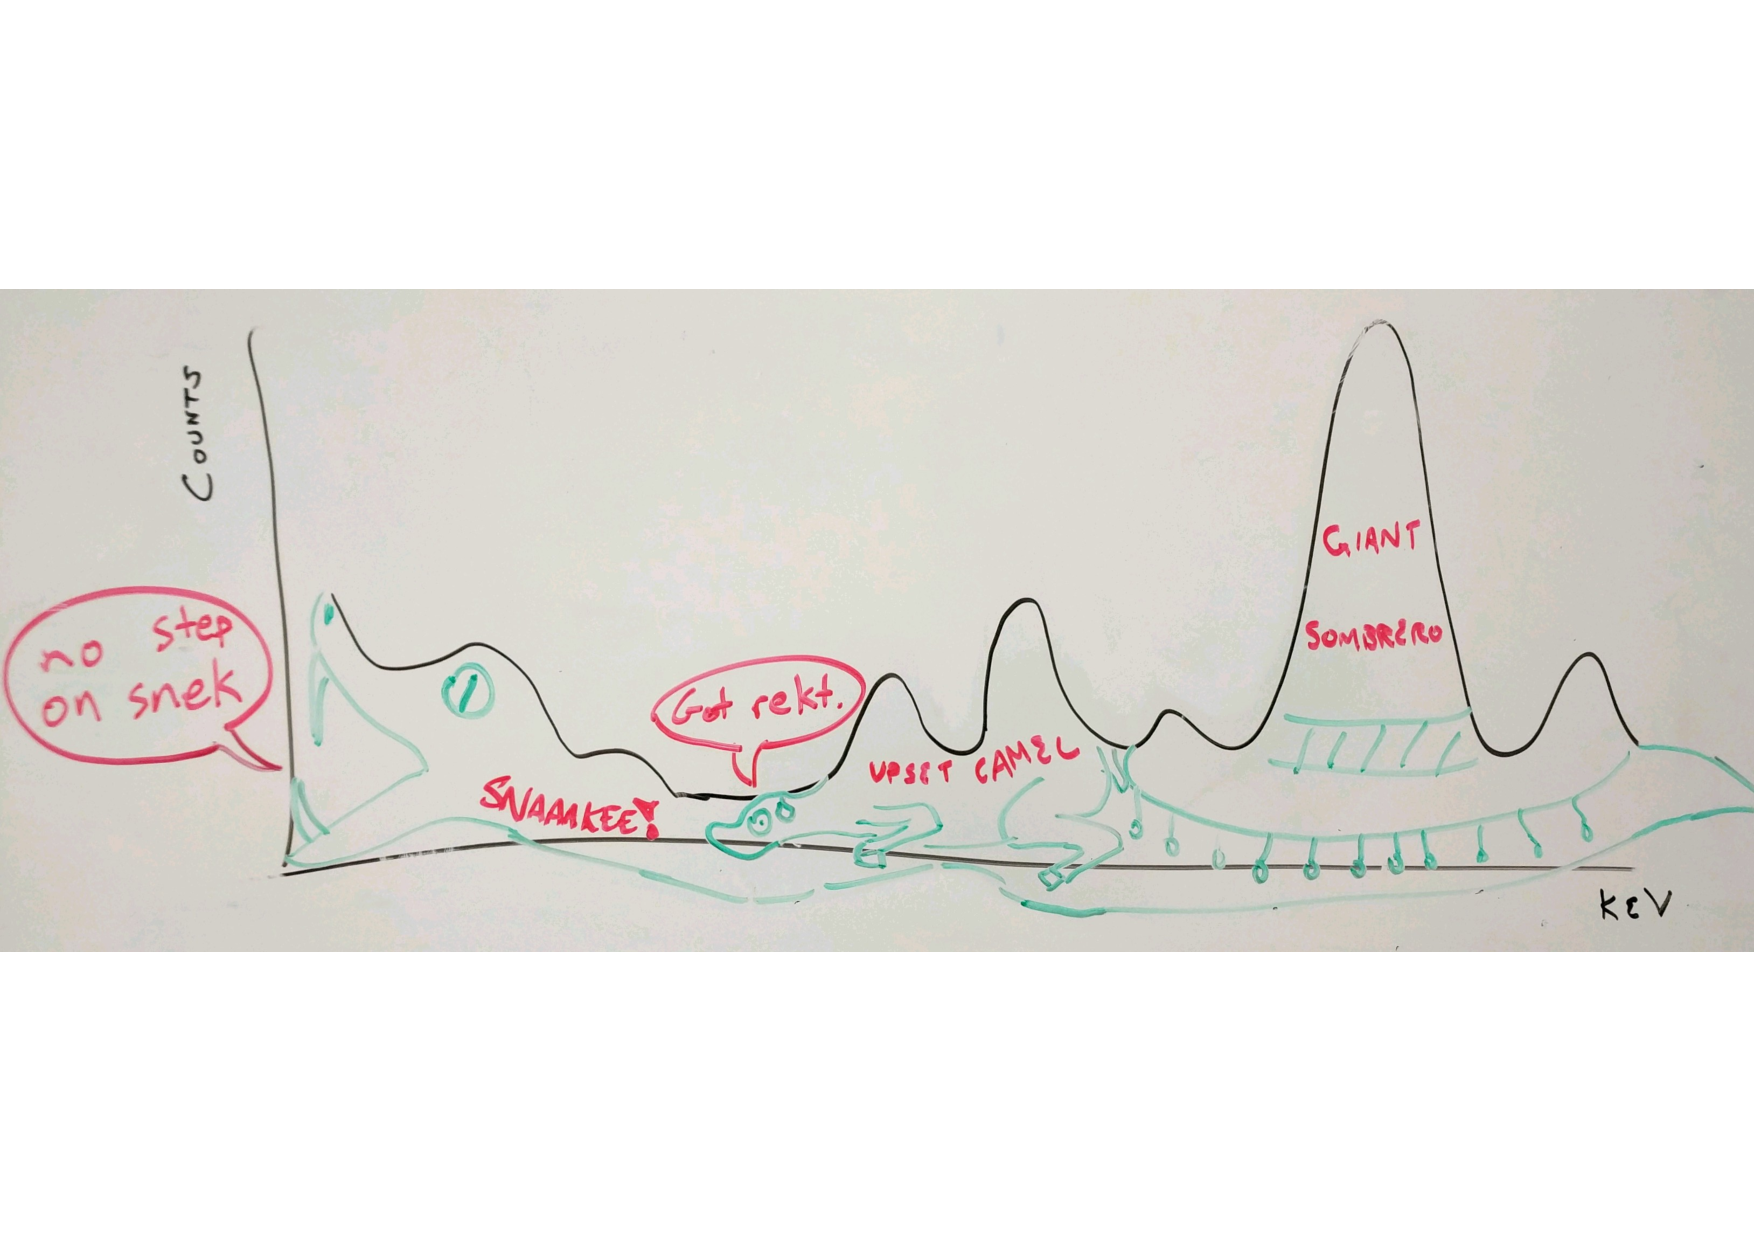
\includegraphics[scale=0.4]{snek.pdf}\\
\begin{multicols}{2}
    Snek on a whiteboard\\
    With camel and sombrero\\
    No step on snek \\
    \columnbreak
    Barium spectrum\\
    Looks like a snek, sombrero\\
    And upset camel
\end{multicols}
\vfill
\hspace{0pt}}

{\centering\dedicationname}

% \raggedright



% These are required, and must be in this order.
\tableofcontents
\listoffigures
\listoftables

% A preface is optional.
%\begin{preface}
%\end{preface}

% It's hard to tell from the information available from the Graduate
% School in Spring 2013 whether or not an acknowledgements section is optional.
%\begin{acknowledge}
%\end{acknowledge}

\mainmatter
%
% Chapter 1
%

%
% Modified by Megan Patnott
% Last Change: Jan 18, 2013
%
%%%%%%%%%%%%%%%%%%%%%%%%%%%%%%%%%%%%%%%%%%%%%%%%%%%%%%%%%%%%%%%%%%%%%%%%
%
% Modified by Sameer Vijay
% Last Change: Tue Jul 26 2005 13:00 CEST
%
%%%%%%%%%%%%%%%%%%%%%%%%%%%%%%%%%%%%%%%%%%%%%%%%%%%%%%%%%%%%%%%%%%%%%%%%
%
% Sample Notre Dame Thesis/Dissertation
% Using Donald Peterson's ndthesis classfile
%
% Written by Jeff Squyres and Don Peterson
%
% Provided by the Information Technology Committee of
%   the Graduate Student Union
%   http://www.gsu.nd.edu/
%
% Nothing in this document is serious except the format.  :-)
%
% If you have any suggestions, comments, questions, please send e-mail
% to: ndthesis@gsu.nd.edu
%
%%%%%%%%%%%%%%%%%%%%%%%%%%%%%%%%%%%%%%%%%%%%%%%%%%%%%%%%%%%%%%%%%%%%%%%%


%
% Chapter 1
%

\chapter{Introduction}

Really, I have no idea what to write here. I suppose I should be writing vaguely about shape coexistence and then explaining key features of it. 

Nuclear structure is broad field, ultimately encompassing the entire nuclear chart, and contributing to other nuclear subfields. Of great interest are phenomena that appear in isolated areas of nuclei, instead of across the chart as a whole. Similarly, phenomena that appear in different sections of nuclei for differing reasons.

Low-lying $0^+$ states are one such phenomenon. In some nuclei, they are caused by particle-hole excitations, in others by intruder states, and in others still, by shape coexistence \citep{wood99:_e0}.

\section{Collectivity/Shape Coexistence}

% and here is the Wood et al 2011 paper.

\section{Electromagnetic Radiation}

\subsection{Internal Conversion}

% gimme dat proof

\subsubsection{E0 Transitions}

% gimme dat proof

\subsection{E0 Transitions for Nuclear Structure}

Electric monopoles are important in studying the nature of nuclear structure. Depending on the strength of the transition, E0 transitions can indicate different types of nuclear structure, ranging from shell model particle-hole pairings to shape coexistence. 

%need to start summarizing that Wood et al 1999 paper.

% % uncomment the following lines,
% if using chapter-wise bibliography
%
% \bibliographystyle{ndnatbib}
% \bibliography{example}


%
% Chapter 2
%

%
% Chapter 2
%

\chapter{Experimental Setup}
\label{chap:setup}

\section{Overview}

For E0 transitions, two types of radiation must be measured: conversion electrons and gamma rays. As conversion electron transitions and intensities are usually tabulated as conversion coefficients, which compare the electron intensities to the respective gamma-rays from the transition, both conversion electrons and gamma-rays must be measured in this experiment. Further, to identify pure E0 transitions, the experiment must show no corresponding gamma rays.

Due to the high level density of nuclei in the rare-earth region, detectors with high resolution are favored for these experiments. The detectors must also be placed in a way that allows for simultaneous measurement of both particles and gamma-rays. For good resolution, high purity germanium (HPGe) detectors are the standard for gamma-rays. For electron detection, silicon-based detectors have the best resolution. The electron energies of interest range from less than 100 keV to over 1 MeV. Standard silicon detectors do not have an energy range that high for electrons, so lithium-drifted silicon (Si(Li)) detectors were be used, which have a higher top-end electron energy.

To make these measurements, three separate experiments were performed at the Nuclear Science Laboratory (NSL) at the University of Notre Dame using the Internal Conversion Electron Ball (ICEBall) Spectrometer paired with two configurations of HPGe detectors: GEORGINA (Figure \ref{fig:georgina_config}) and Clovershare (Figure \ref{fig:clovershare_config}). 

\begin{figure}
    \centering
    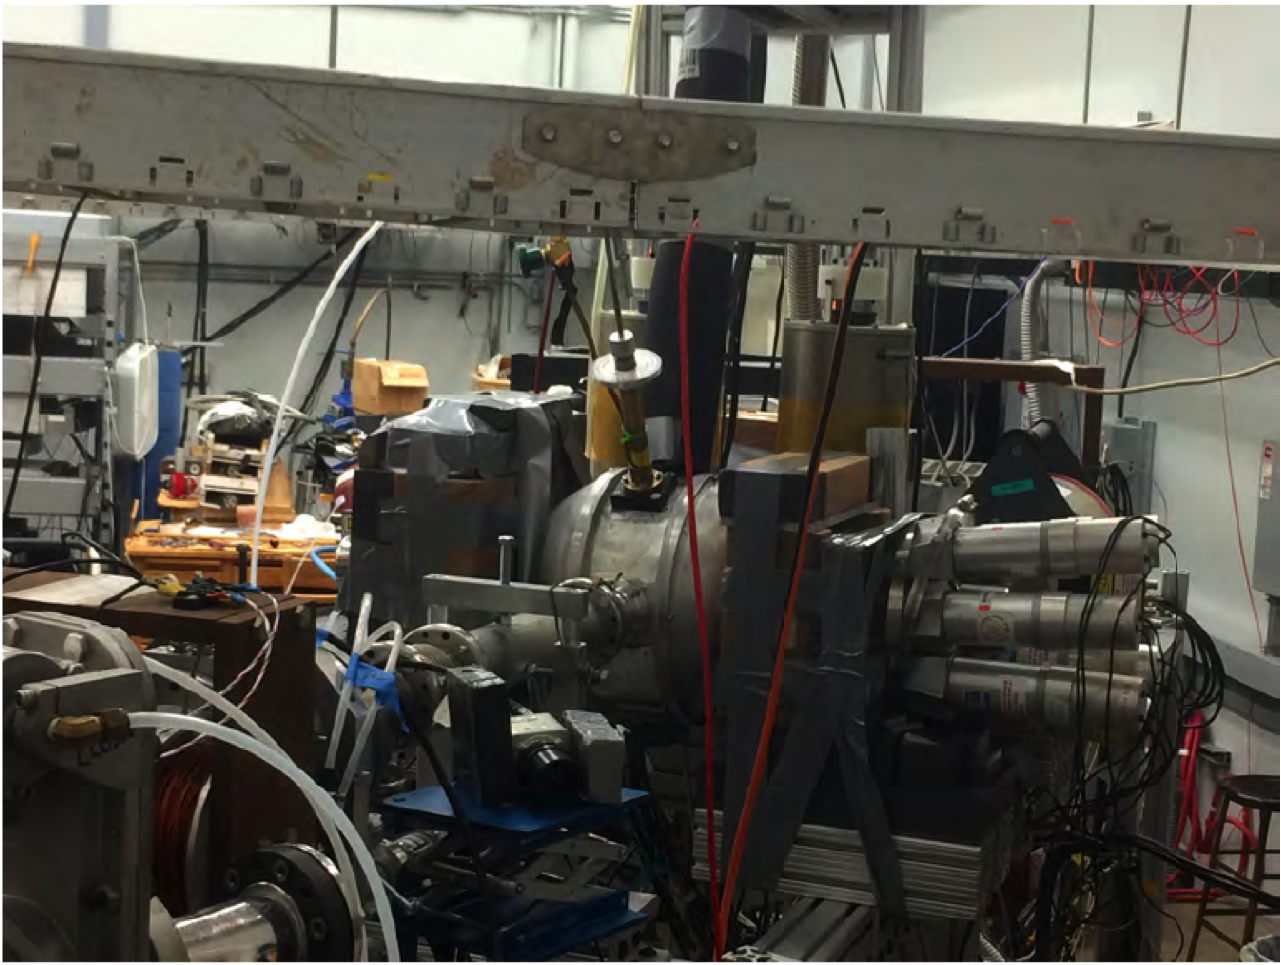
\includegraphics[scale=0.6]{Setup_Figs/ICEBall-2014.png}
    \caption{Image of the assembled experimental configuration with GEORGINA. One HPGe detector has BGO crystals around it.}
    \label{fig:georgina_config}
\end{figure}

\begin{figure}
    \centering
    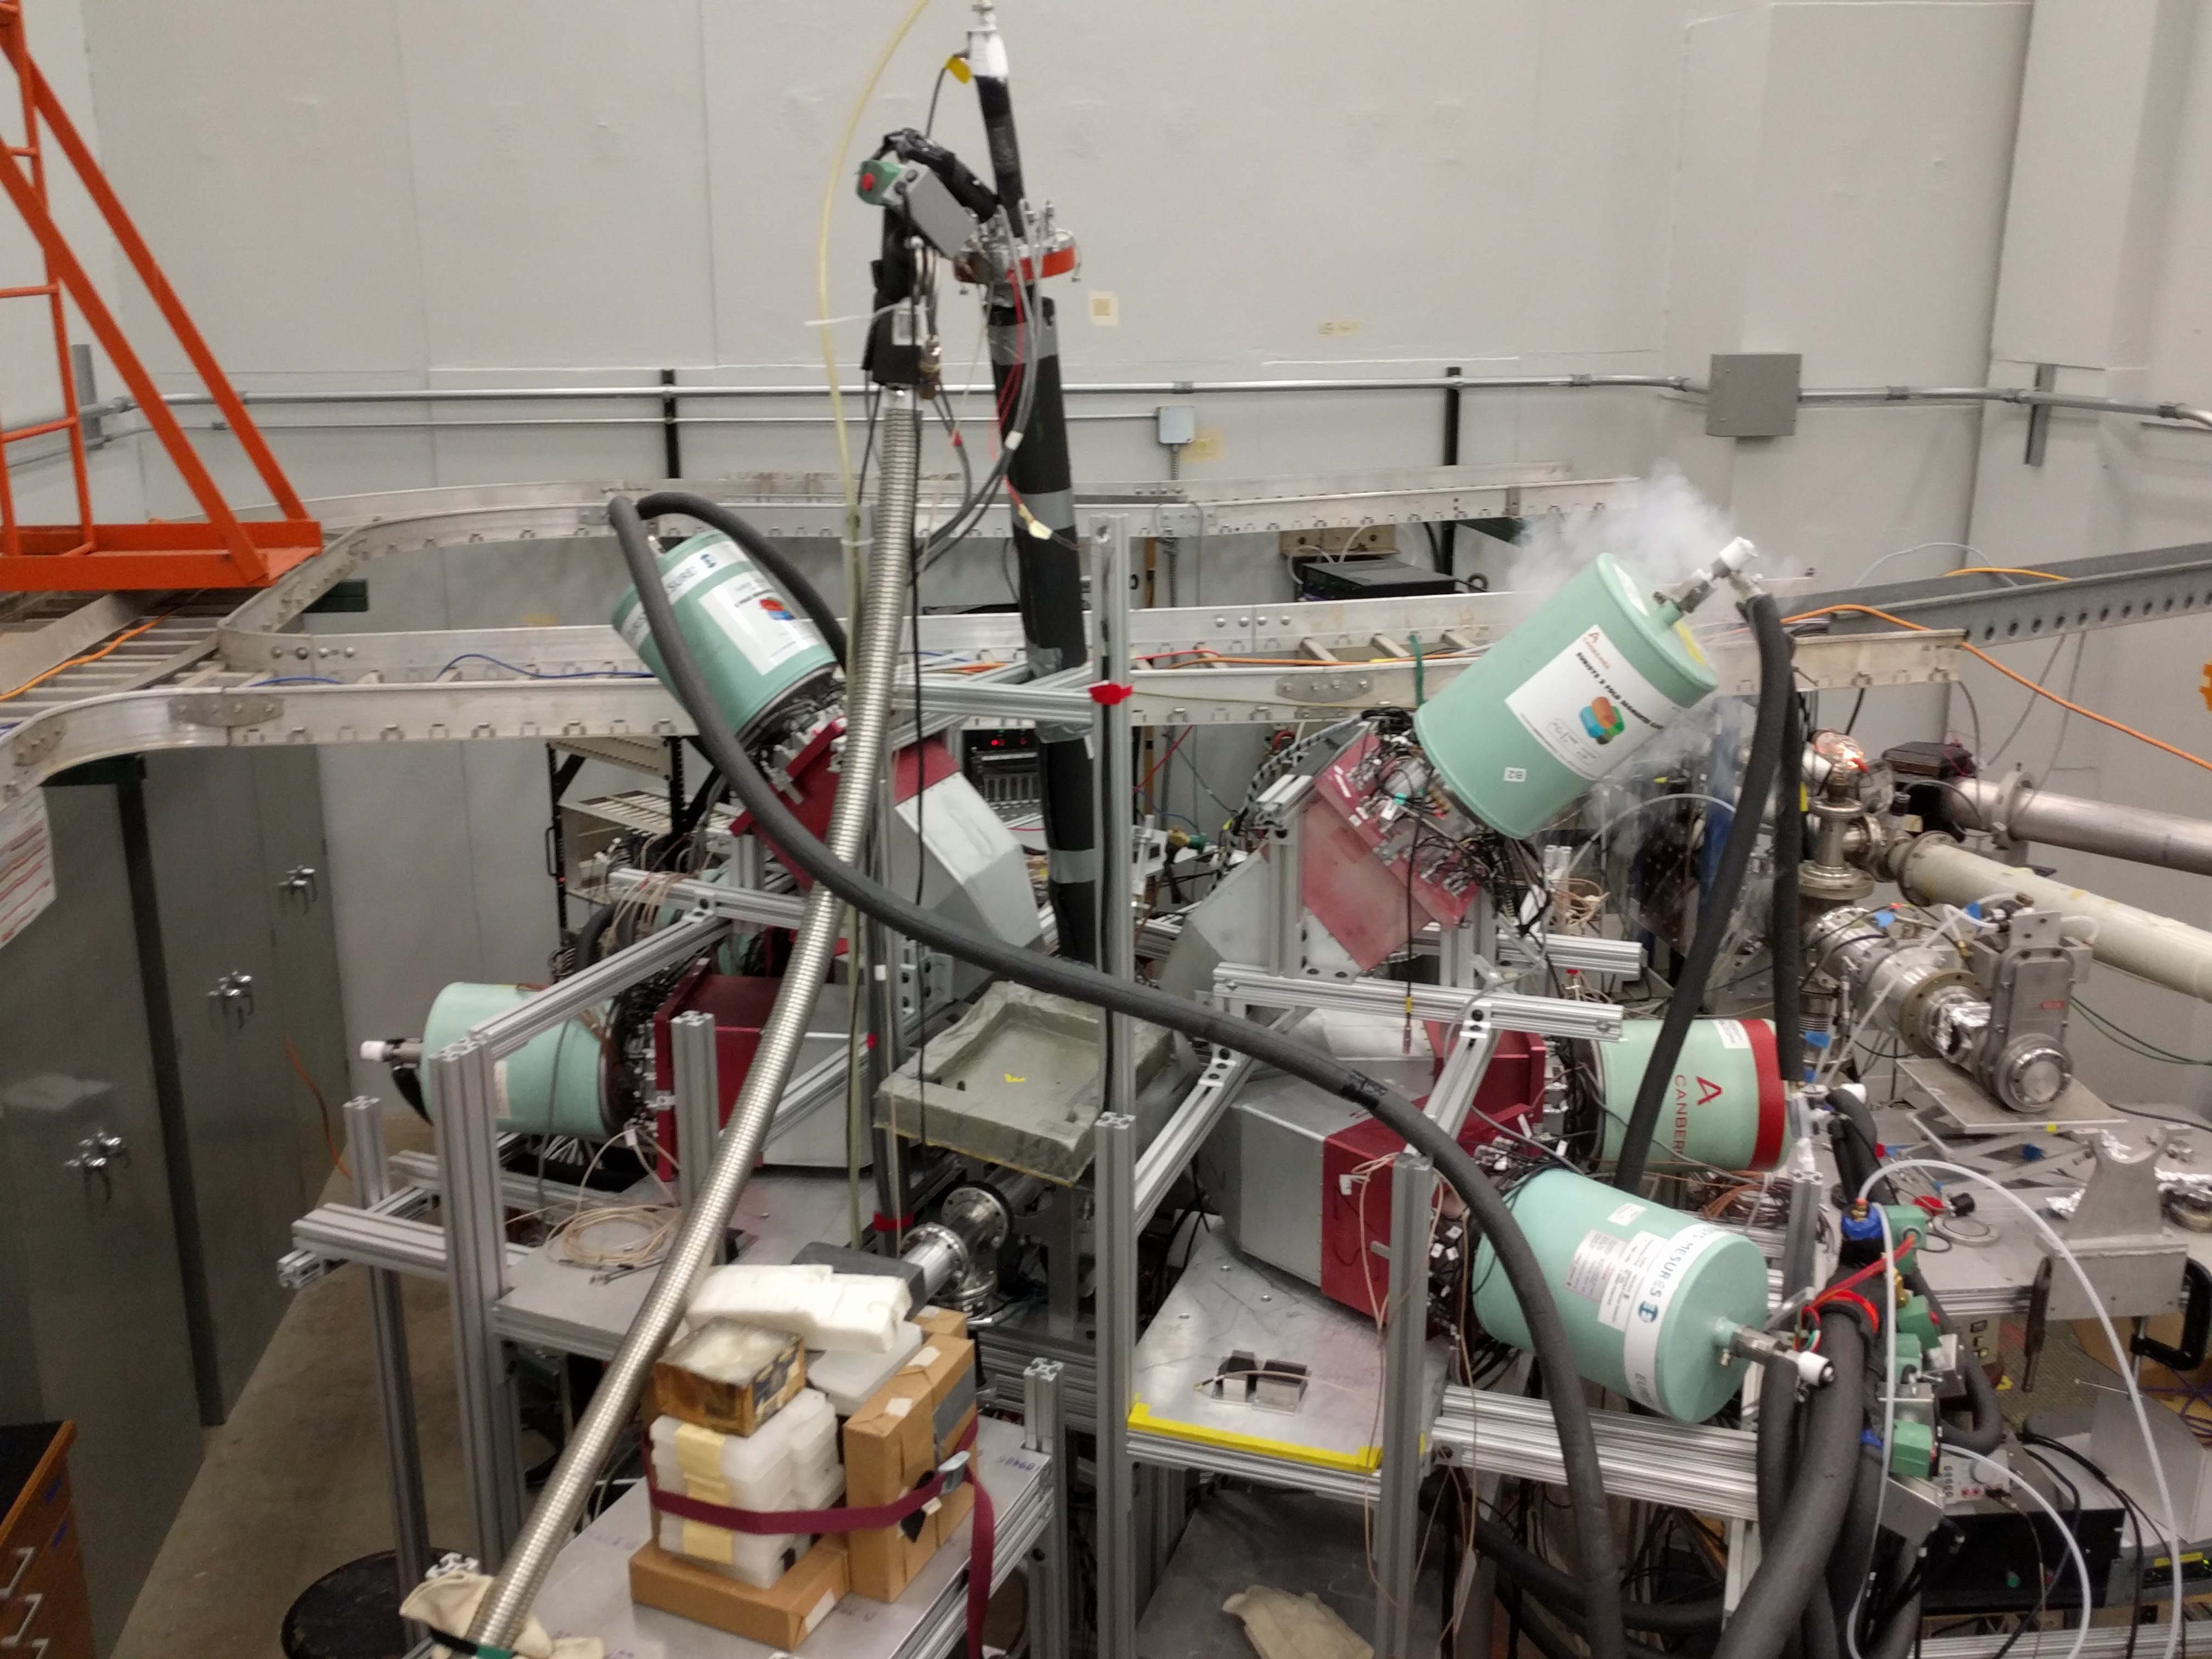
\includegraphics[scale=0.1]{Setup_Figs/IMG_20160311_192243.jpg}
    \caption{Image of the assembled experimental configuration with Clovershare. One HPGe detector is not visible from this angle.}
    \label{fig:clovershare_config}
\end{figure}

The $(\alpha,2n)$ reaction favors populating states of low, even-$J$ and positive parity. These states, including the $0^+$ states, are the ones of interest in this study, making this a natural reaction to select for the experiment. The $Q$ value for this reaction is -14.774 MeV for $^{154}$Gd and -13.638 MeV for $^{156}$Gd, meaning an alpha beam of the necessary energy for the reaction to occur is well within the capability of the NSL.

A Sm$(\alpha,2n)$Gd reaction was used with different enriched targets to create the desired Gd isotope, with an $\alpha$ beam of 20 MeV. A bunched beam was used to create timing for coincidence identification. This beam energy was determined by a measurement using a natural Sm target, with ICEBall and two neutron detectors. TALYS was run to determine a range of energies to maximize the cross section of the desired reaction, while minimizing the neutron flux, as neutrons can damage HPGe detectors. Figure \ref{fig:alpha-neutron} shows the cross sections for the $(\alpha,xn)$ reactions for $^{154}$Sm in the $\alpha$ energy range of interest. Beam energies from 16 MeV to 21 MeV were tested. Measurements were done at 1 MeV intervals. The cross section was calculated using conversion electron measurements from ICEBall, and compared with the neutron flux at that energy.

\begin{figure}[t]
    \centering
    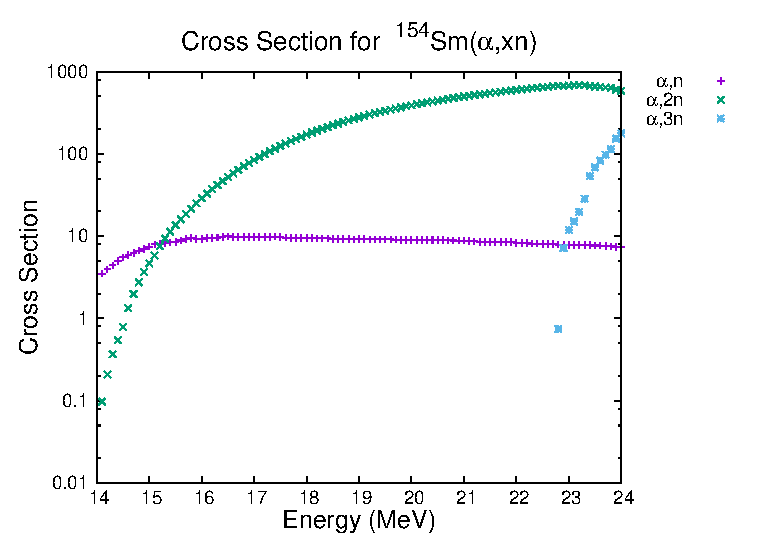
\includegraphics[scale=1]{Setup_Figs/alpha-n-comp.eps}
    \caption{Comparison between the cross sections of the $(\alpha,xn)$ reactions on $^{154}$Sm, calculated using Talys\citep{koning07:_talys}. The fewer neutrons being emitted, the lower the energy before the reaction occurs. Maximizing the cross section with respect to the neutron flux can be done by finding an energy where the desired reaction, $(\alpha,2n)$ can be maximized, while minimizing the $(\alpha,n)$ and $(\alpha,3n)$ reactions. Specifically, this means finding an energy before the $3n$ reaction has significant strength, while maximizing the $2n$ reaction, as the $n$ reaction is nearly the same across the energy regime of interest.}
    \label{fig:alpha-neutron}
\end{figure}

Two different forms of electronics were used for the data acquisition system. The data acquisition systems used were based on the NSCL DAQ\citep{nscl:_daq,prokop14:_nsclddas}. The electronics used with GEORGINA were shaped by NIM modules before going through ADC VME modules to the computer \citep{mesytec:_ADC,caen:_TDC}. The Clovershare data used the XIA Pixie-16 modules, which take the place of the NIM and VME modules for shaping and converting the signals to digital data \citep{xia:_pixie}.

The digital files were converted to files for the analysis software using \texttt{evt2root} \citep{smith14:_evt2root}. Analysis, reported in chapter \ref{ch:analysis}, was done using the CERN Root Data Analysis Framework and Radware \citep{brun97:_root,radford00:_radware}.

\section{Nuclear Science Laboratory at Notre Dame}

The Nuclear Science Laboratory at the University of Notre Dame has been in operation since the 1934, with accelerators in operation since 1937. Currently, the NSL operates locally with three accelerators: the FN Tandem, the 5 MV Single-Ended Sta. Ana accelerator, and the 3 MV 9S Tandem. There is also a fourth accelerator, a 1 MV machine called CASPAR, located in the Homestake Mines in South Dakota. The experiments in this dissertation were performed on the FN Tandem. Figure \ref{fig:NSL} is the current layout of the NSL. The accelerator in the top right of the figure is the FN Tandem.

The FN Tandem has two ion sources: the Helium Ion Source (HIS) and the Multi-Cathode Source of Negative Ions Using Cesium Sputtering (MC-SNICS). Most elements can absorb the electrons from cesium to create negative ions. Helium cannot and needs a special source, as discussed below. For the experiments described, the HIS was used.

Due to the electron binding energy of helium, the HIS uses a duoplasmatron. Within the duoplasmatron, a thin tungsten wire is heated while surrounded by the source gas (helium). The tungsten wire emits electrons, and positively ionizes the helium. This helium is extracted from the duoplasmatron and focused by an einzel lens, where it then goes through the lithium charge exchange. This section of the HIS works as a small two stage acceleration system, although the charge exchange works added electrons instead of stripping them. The positively charged ions are accelerated through a lithium vapor, and some gain electrons, becoming neutral or negatively charged. Those ions that become negatively charged are accelerated out the other end of the HIS, before being sent to the FN Tandem. Figure \ref{fig:HIS} is a schematic of this system.

\begin{figure}[t]
    \centering
    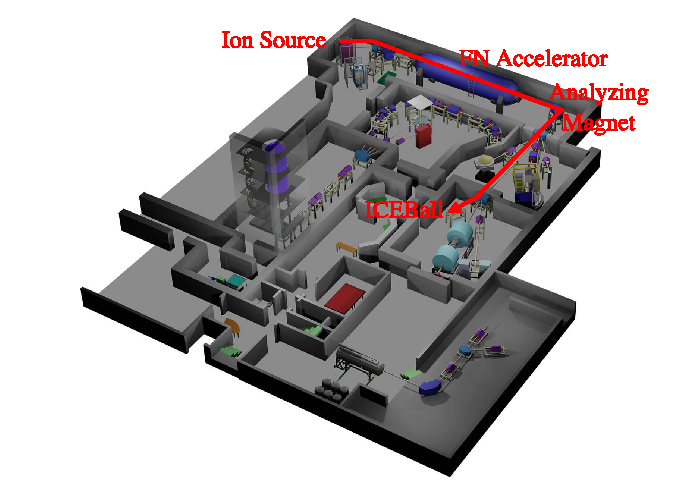
\includegraphics[scale=1.25]{Setup_Figs/NSL_2018_Layout.eps}
    \caption{Current layout of the Nuclear Science Laboratory at Notre Dame. The red line indicates the path taken by the beam, from ion source, through the accelerator and analyzing magnet, before being sent to ICEBall.}
    \label{fig:NSL}
\end{figure}

The FN Tandem has been in operation since 1968. It is a Van de Graaff. Charging chains carrying a static charge deposit the charge on a terminal in the center of the machine. The charging chains is a pelletron type, upgraded from the original insulated rubber belt system in 2000. The pelletron chain consists of metal pellets connected using nylon, allowing for each pellet to be electrically isolated as it carries electrical charge to the terminal \citep{nec:_pelletron}. The beamline is kept at vacuum, but the area outside of the beamline, but within the accelerator tank, is filled with a mixture of CO$_2$ and dry nitrogen gas, at approximately 200 PSI. To create a more uniform acceleration field, the terminal is brought to ground along the beamline using resistor-lined tubes. The resistors used create a uniform electrical field down the tube, allowing for uniform acceleration.

It is known as a tandem because the system is a two-stage acceleration. Negatively charged ions enter the system, accelerating toward a positively charged terminal shell. Inside of the shell, the ions go through carbon stripping foils 3 $\mu g/cm^2$ thick, becoming positively charged as electrons are pulled off. The ions then accelerate away from the terminal for the second stage. The total energy gained by the ions is the terminal voltage times the quantity of one plus the final charge state.

\begin{figure}
    \centering
    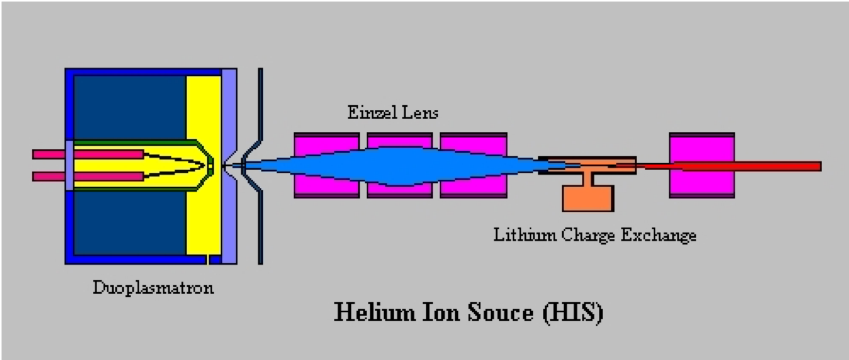
\includegraphics[scale=0.75]{Setup_Figs/HIS.png}
    \caption{A schematic of how the Helium Ion Source works.}
    \label{fig:HIS}
\end{figure}

After being sent through the accelerator, the beam goes through the analyzing magnet. This magnet is set for the specific species, energy, and charge state to bend 90 degrees to the experimental set ups.

\section{Beam Production}

Because of the use of HPGe detectors in an $(\alpha,2n)$ reaction, the neutron flux must be minimized in comparison to the cross section of the reaction, as the $(\alpha,n)$ reaction is also open. The neutrons being produced will interact with everything, including the HPGe detectors, which can be damaged by the $(n,\gamma)$ reaction on germanium. To do this, a range of energies to test were selected by looking at theoretical cross sections in Talys\citep{koning07:_talys}. These energies were then tested with natural Sm targets, ICEBall, and two liquid scintillators to detect neutrons.

Samarium, as with many even-Z elements in the lanthanide region, has many stable isotopes. A total of five stable isotopes of Samarium exist, with two other isotopes being long-lived. Table \ref{tab:nat_Sm} summarizes the abundances and lifetimes of the various isotopes found in natural Samarium. The two isotopes used our enriched targets are the ones that have the highest natural abundances, $^{152,154}$Sm.

\begin{table}[]
    \centering
    \begin{tabular}{c|c|c}
    \toprule
         Isotope & Lifetime (y) & Abundance (\%)  \\
         \hline
         $^{144}$Sm & Stable & 3.08 \\
         $^{147}$Sm & $1.06\times10^{11}$ & 15.00 \\
         $^{148}$Sm & $7\times10^{15}$ & 11.25 \\
         $^{149}$Sm & Stable & 13.82 \\
         $^{150}$Sm & Stable & 7.37 \\
         $^{152}$Sm & Stable & 26.74 \\
         $^{154}$Sm & Stable & 22.74 \\
         \bottomrule
    \end{tabular}
    \caption{Isotope Distribution of Natural Samarium}
    \label{tab:nat_Sm}
\end{table}

\subsection{Talys Calculations}

Talys \citep{koning07:_talys} is code for simulation of nuclear reactions dynamically with neutrons. Cross sections can be estimated using Talys to guide where an experiment may want to run to optimize production, as is the case presently. 

Both natural and enriched samarium targets were used and modelled within Talys. A range of energies, from 14 MeV to 24 MeV $\alpha$-particles were run. These energies allowed a large number of potential reaction products from elastic, inelastic, transfer, and knockout reactions. Figure \ref{fig:talys} is a visual summary of the strongest modelled reactions in the natural samarium target. It was decided to test the energies between 16-21 MeV.

\begin{figure}[t]
    \centering
    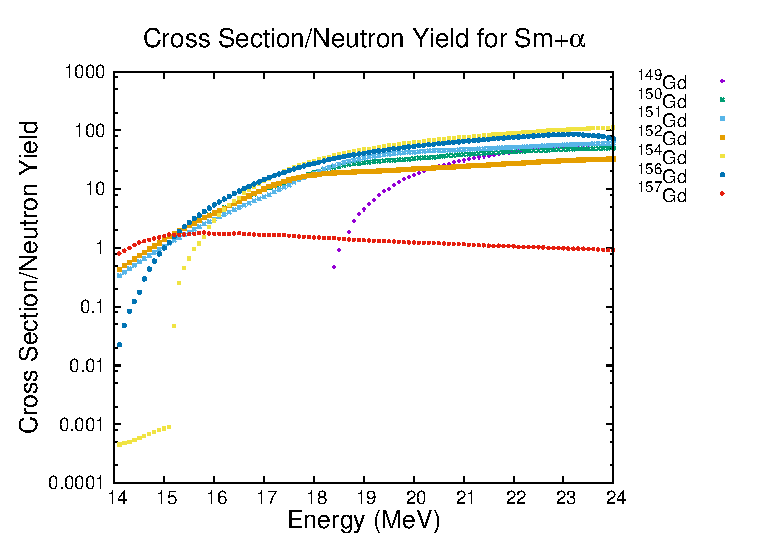
\includegraphics[scale=1]{Setup_Figs/Talys_Ratio.eps}
    \caption{Talys calculation of the highest cross sections divided by the total neutron yield in the natural Samarium target. Only the largest contributors are included, as there are a large number of products possible between the isotopes of Samarium in the target and the reactions channels open for each. All of the largest contributors are Gadolinium isotopes. The ratios for the isotopes of interest appear to plateau around 20-22 MeV.}
    \label{fig:talys}
\end{figure}

\subsection{Test Analysis and Results}

To test these Talys calculations and determine the best running energy, the cross section and neutron flux had to be measured at each energy without the use of the HPGe detectors. This was done using a natural samarium target. ICEBall was used to measure the cross section by examining the K-electrons from ground-state band transitions in the reactions of interest, as the ground-state band is the most significantly populated band in the reaction. The DAQ described in section \ref{sec:GEORGINA_electronics} was used. Spectra from ICEBall were fit using the methods described in \ref{sec:fitting}. The peaks were identified under the assumption the ground-state band transitions would be the strongest peaks in the spectra, and populate quickly. 

The neutrons were measured using two NE213 liquid organic scintillators. In these detectors, it is possible to do pulse shape discrimination, as the neutrons have longer decay times than the gammas in these detectors due to the nature of the interaction with the scintillating liquid \citep{knoll00:rad_det_meas}. This produces longer trails in the detectors, leading to different decay shapes, see Figure \ref{fig:pulse_discrimination}. 

\begin{figure}
    \centering
    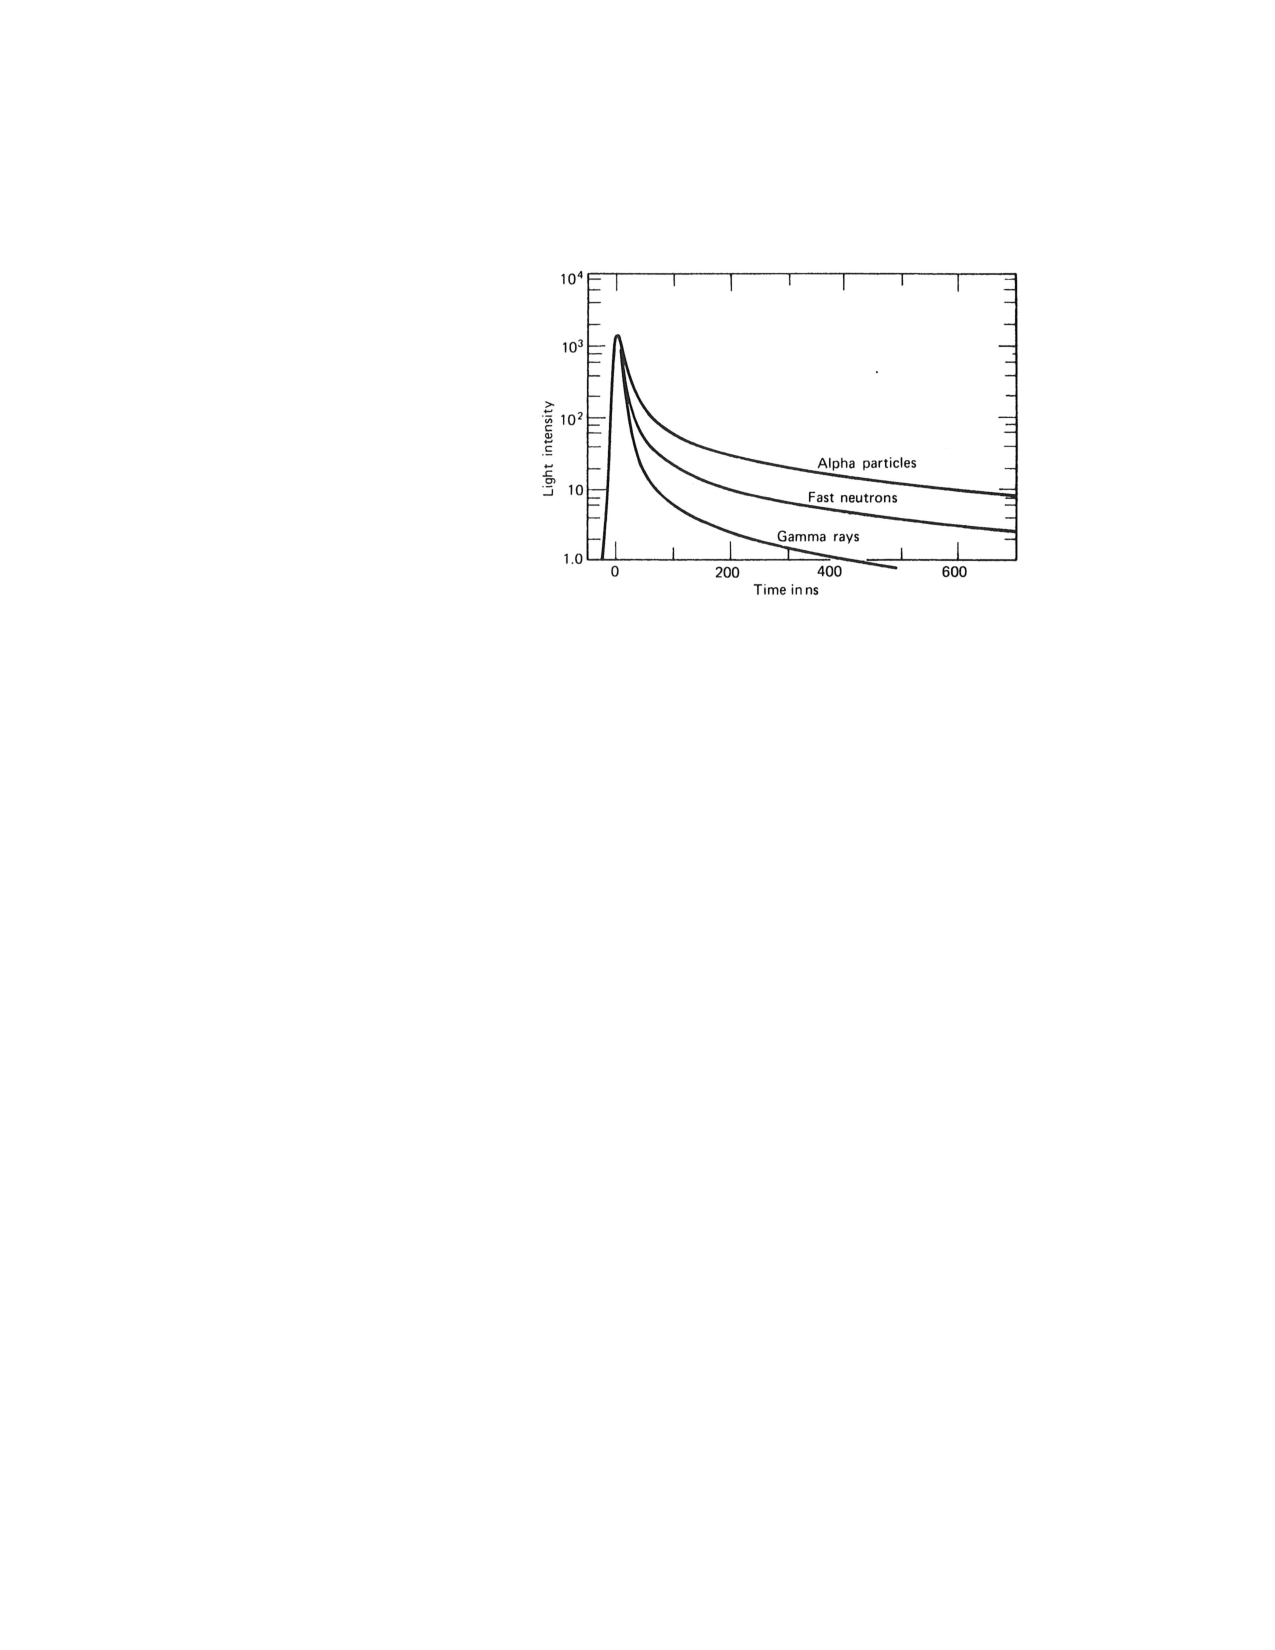
\includegraphics{Setup_Figs/pulse_shape.pdf}
    \caption{A cartoon illustration of pulse shape based on radiation type, in the same detecting material. The different types of radiation interact with the detecting material creating a fast and slow excitation. The ratio of these fast and slow excitations is based on the radiation, and expressed in the length of the decay tail. Picture taken from \citep{knoll00:rad_det_meas}.}
    \label{fig:pulse_discrimination}
\end{figure}

By plotting the pulse height against the decay tail time, neutrons and gammas can be separated. In this setup, this was done by sending the signal to a Mesytec MPD-4 (Multi-channel Pulse Discriminator) \citep{mesytec:_PSD}. This is a module built for pulse discrimination. It splits the signal, amplifies for the pulse height, and sends the other signal to a constant fraction discriminator (CFD), which converts the value to an amplitude using a time to analog converter (TAC). A CFD works by measuring the time it takes for a pulse to decrease to a fraction of its original height. Both of these signals (the pulse amplitude and the TAC amplitude) are recorded in the data. Plotting these values in a two-dimensional plot distinguishes the gammas and neutrons, as in Figure \ref{fig:neutron}. There is a threshold cut off that removed most gammas from the spectrum.

\begin{figure}
    \centering
    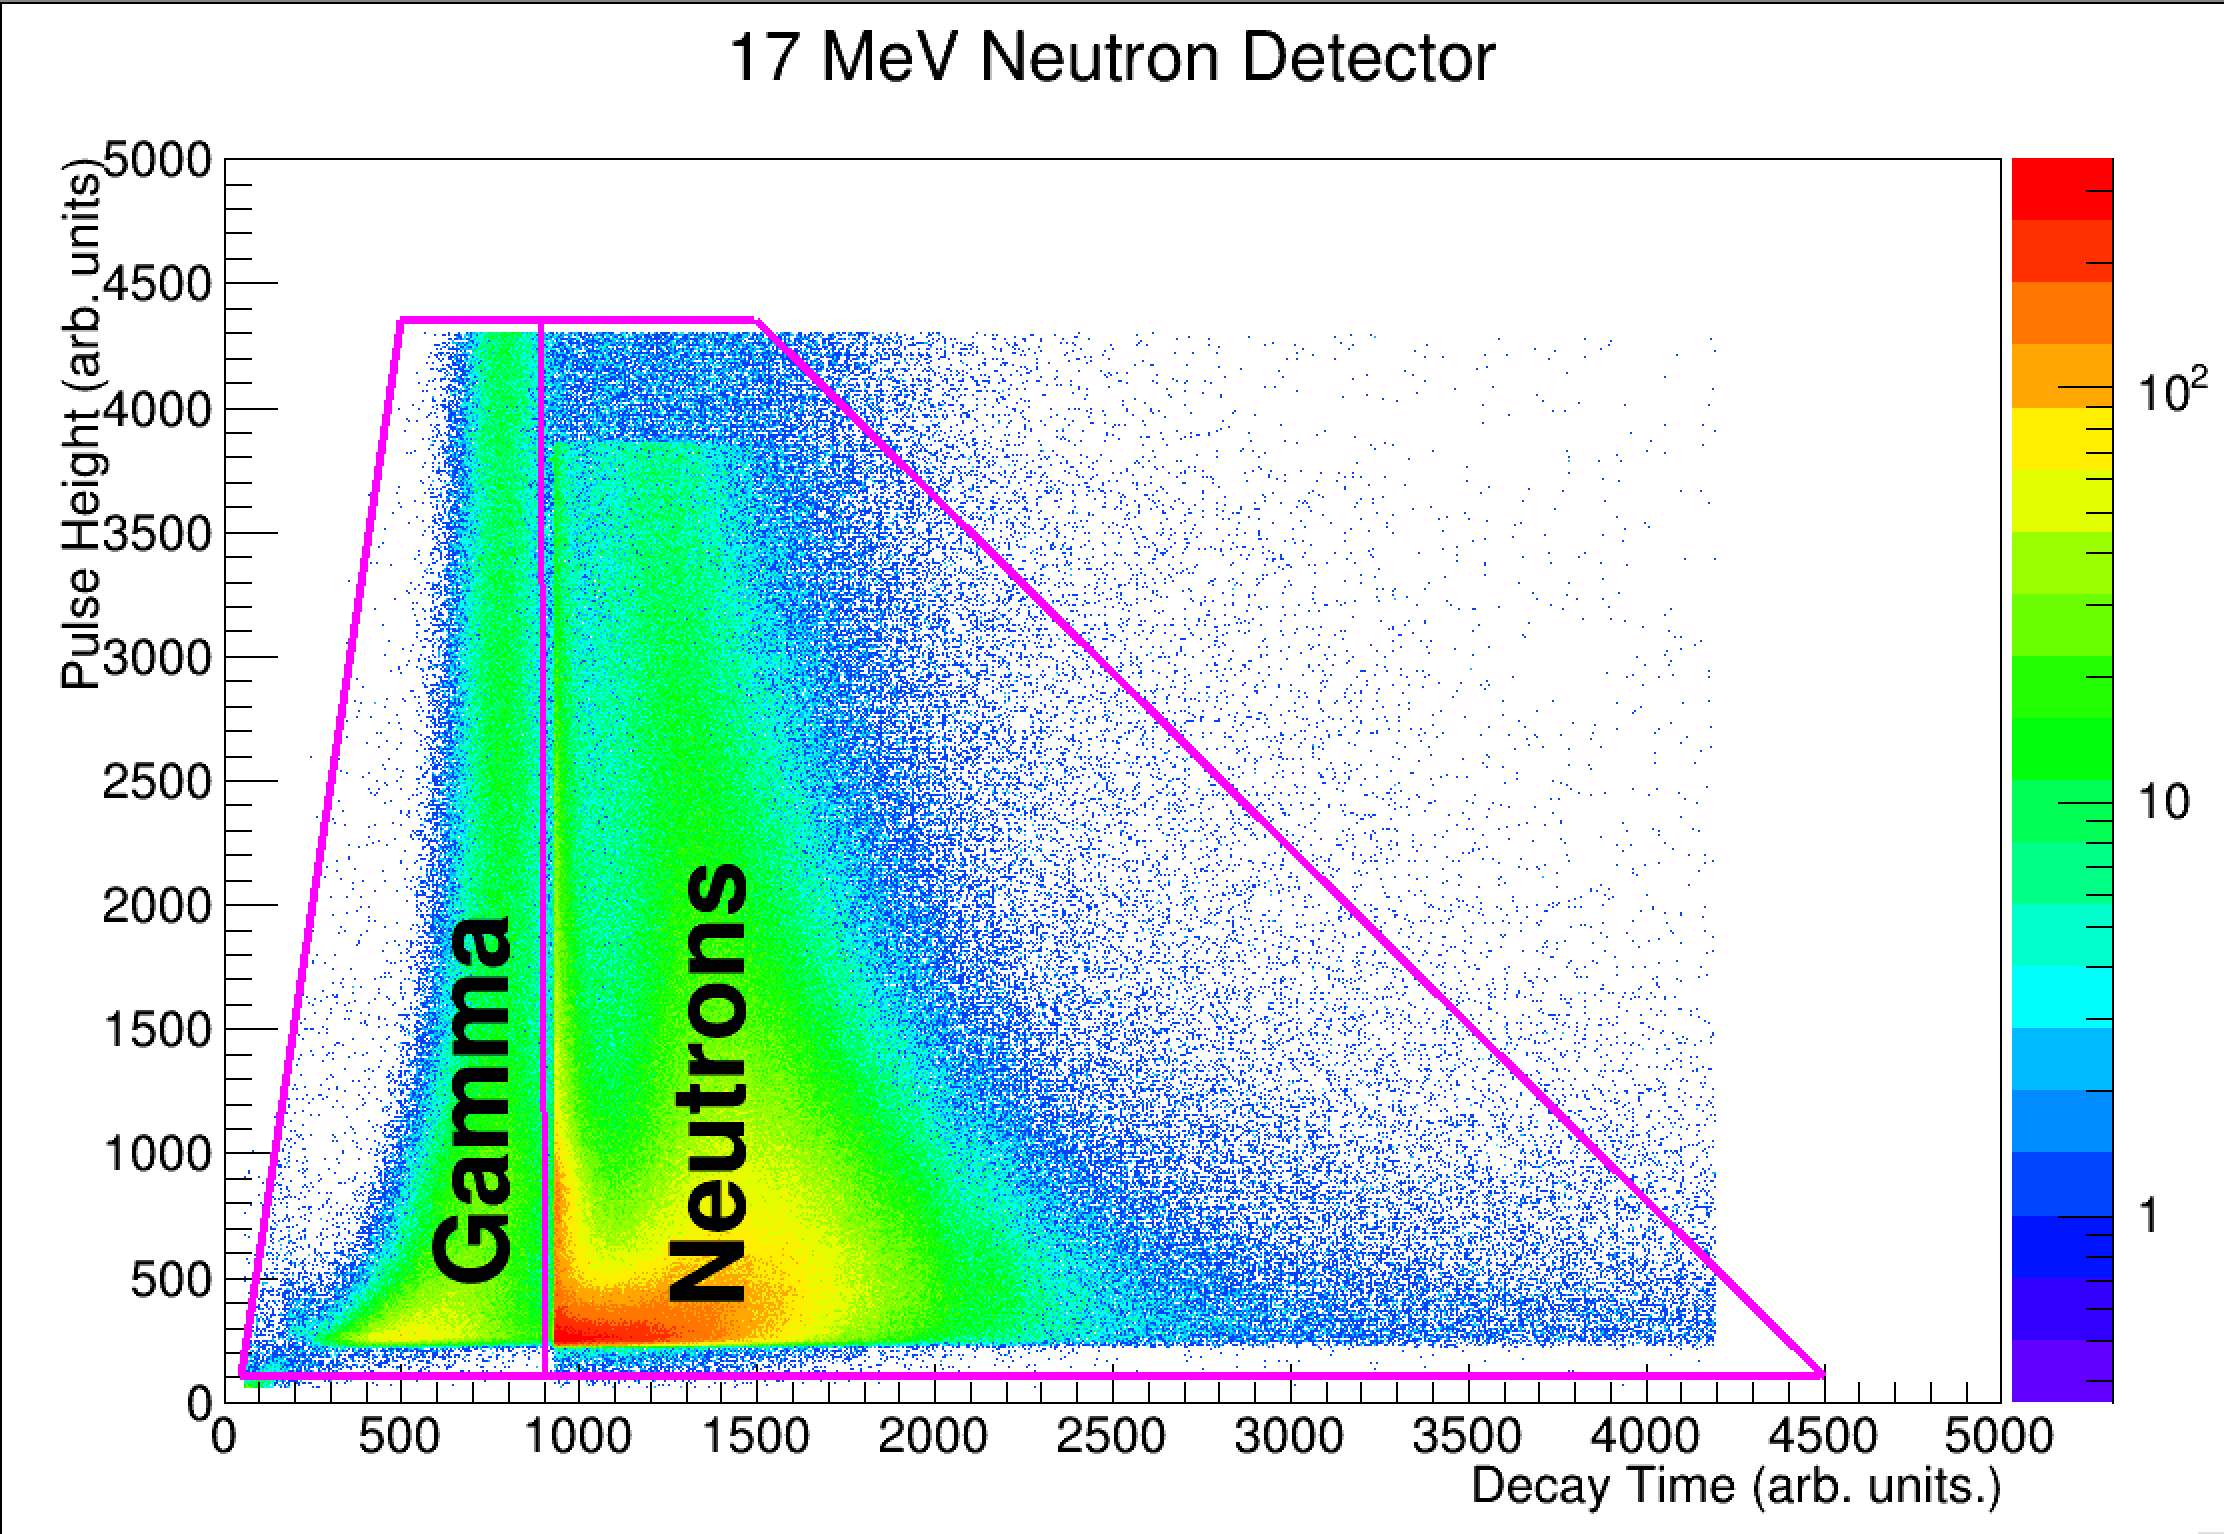
\includegraphics[scale=0.7]{Setup_Figs/17MeVNeutron.eps}
    \caption{Plot of the pulse height vs the decay time in the NE212 detectors. Two clear areas are seen. The leftmost, with the shorter decay time, is the gammas, while the more spread out peak on the right is neutrons.}
    \label{fig:neutron}
\end{figure}

Once the detectors were calibrated, each energy was run, with a total of four different targets across six energies. For each energy, the peaks in the electron spectra were identified with their respective isotopes, working under the assumption that only the lowest-lying states and the ground-state band would be populated significantly enough to see the electrons. These peaks are representative of the reaction cross section for that isotope. The K-electron of the $4^+\rightarrow2^+$ ground state transition for both nuclei of interest was clearly visible and clean at all energies, listed in Table \ref{tab:neutron_electron}. These K-electrons were used for the cross-section calculation.

\begin{table}[]
    \centering
    \caption{$4^+\rightarrow2^+ K-Electrons by Isotope$}
    \begin{tabular}{c|c}
    \toprule
         Isotope & Energy (keV)  \\
         \hline
         $^{154}$Gd & 197 \\
         $^{156}$Gd & 149 
         \bottomrule
    \end{tabular}
    \label{tab:neutron_electron}
\end{table}


To calculate the cross section, the formula

\begin{equation}
    \sigma=\frac{Yield}{\delta x*Q*\epsilon}
    \label{eq:xs}
\end{equation}

was used, where $\delta x$ is the target thickness, $Q$ is the integrated charge, and $\epsilon$ is the efficiency of the Si(Li) detector at the electron energy. The $Yield$ is the area under the curve.

This then had to be compared with the neutron production cross section. A bunched beam was used to get a time-of-flight. Calculating the neutron flux was done using the formula

\begin{equation}
    \sigma_n = \frac{Neutrons}{\delta x*Q}
\end{equation}

where $\delta x$ and $Q$ are the same as used for the cross section. The neutron yield is obtained by pulse shape discrimination, as seen in Figure \ref{fig:neutron}. The left-most line is the gamma-flash that comes from the prompt gammas. The secondary gathering of counts, to the right, is the neutron peak. This area can be integrated over to get the number of neutrons seen during the run.

Table \ref{tab:neutrons} summarizes the results at each energy. Note, that the cross section is not reflective of the full cross section of the isotopes, but of the K-electrons for that transition. This ratio, of the cross-section to the neutron flux, was ultimately used to determine the running energy. The two higher energies, 20 and 21 MeV, have a ratio that agrees within error for both isotopes, indicating a plateau, in agreement with the expectation from Talys. Ultimately, 20 MeV was chosen for two reasons: to minimize any higher energy reaction channels, and because the neutron flux was lower in rate.

\begin{table}[]
    \centering
    \begin{tabular}{c|c|c|c|c|c}
        \toprule
        & \multicolumn{2}{c|}{Cross Section (mb)} & Neutron Flux & \multicolumn{2}{c}{Ratio ($\sigma/\Phi_n$)} \\
        Energy (MeV) & $^{154}$Gd & $^{154}$Gd & (neutrons/s) & $^{154}$Gd & $^{154}$Gd \\
        \hline
        16 & 0.126 (13) & 0.334 (25) & 1.247 (4) & 0.101 (10) & 0.268 (20)\\
        17 & 0.554 (54) & 1.273 (91) & 2.142 (13) & 0.259 (25) & 0.594 (43)\\
        18 & 3.124 (133) & 5.427 (233) & 4.281 (30) & 0.730 (31) & 1.268 (55)\\
        19 & 3.030 (172) & 5.327 (217) & 4.205 (25) & 0.721 (41) & 1.267 (52)\\
        20 & 5.618 (167) & 9.438 (275) & 5.806 (36) & 0.968 (29) & 1.626 (48)\\
        21 & 7.438 (267) & 12.827 (419) & 7.410 (54) & 1.004 (37) & 1.731 (58)\\ 
        \bottomrule
    \end{tabular}
    \caption{Summary of Energy Tests}
    \label{tab:neutrons}
\end{table}

\section{Electron Detection}

Silicon detectors are a commonly used particle detector, with good energy resolution. The detectors are semiconductors, using a $p-n$ junction to create a depletion region, which becomes the active detection region\citep{knoll00:rad_det_meas}. Semiconductors have a bandgap around 1eV. A cartoon of the bandgap can be seen in Figure \ref{fig:bandgap}. The $p-n$ junction takes two semi-conductor materials, one of $p$-type (an excess of holes in the valence band) and one of $n$-type (an excess of electrons in the conduction band) together. The holes and electrons mix, creating a depletion region, which becomes the active detection area. This region can be enlarged to some extent by putting a bias across the detector.

\begin{figure}
    \centering
    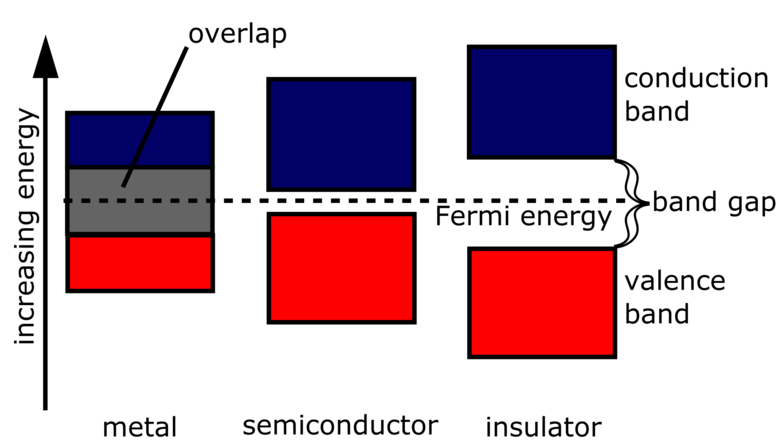
\includegraphics[scale=0.5]{Setup_Figs/semiconductor.png}
    \caption{Cartoon of how the bandgap works for insulators, conductors, and semiconductors. Insulators have a large band gap, conductors overlap, and semiconductors have a small bandgap.}
    \label{fig:bandgap}
\end{figure}

Because electrons are much more penetrative than protons or alphas of the same kinetic energy, it takes much more material to fully stop electrons. Silicon detectors only have active regions of 1mm-2mm thick, due to impurities, and cannot be made thick enough for the purposes of measuring electrons in the energy range of interest. Lithium-drifted silicon, colloquially Si(Li), detectors operate under the same principles as silicon detectors, but can be manufactured with larger depletion regions and a larger detectable energy range of electrons. These work by specifically introducing impurities, or doping, in this case lithium, to the detector, drifting it to create a $p-i-n$ junction. The $i$ region is also known as the intrinsic region, and is created by the drifting of the lithium, creating a highly purified region. The thickness of these detectors is only limited by the distance across which the lithium can be successfully drifted.

\subsection{Internal Conversion Electron Ball Spectrometer}

The Internal Conversion Electron Ball Spectrometer (ICEBall) was developed at the University of Pittsburgh by Metlay et al. \citep{metlay92:_iceball_comm,metlay93:_iceball_comm}. Originally at the Spin Spectrometer at Oak Ridge National Laboratory, it was later stationed at the Wright Nuclear Structure Laboratory at Yale University with the YRAST Ball, until being brought to the University of Notre Dame and stationed in the Nuclear Science Laboratory West Target Room, on a dedicated beamline \citep{battaglia15:_iceball_176lu}.

Originally designed to go inside of large gamma detector arrays, ICEBall consists of six mini-orange spectrometers, cooled using liquid nitrogen for ideal energy resolution. The liquid nitrogen is administered using an autofill system with two thermal sensors for a start and stop signal. When the sensor closest to the detectors warms enough, liquid nitrogen is pumped into the system. A second sensor at the top of the dewar is used to stop the fill of liquid nitrogen before it overflows. This system fills in 15 to 20 minute intervals. ICEBall can be seen in Figure \ref{fig:open_iceball}, open for servicing.

\begin{figure}
    \centering
    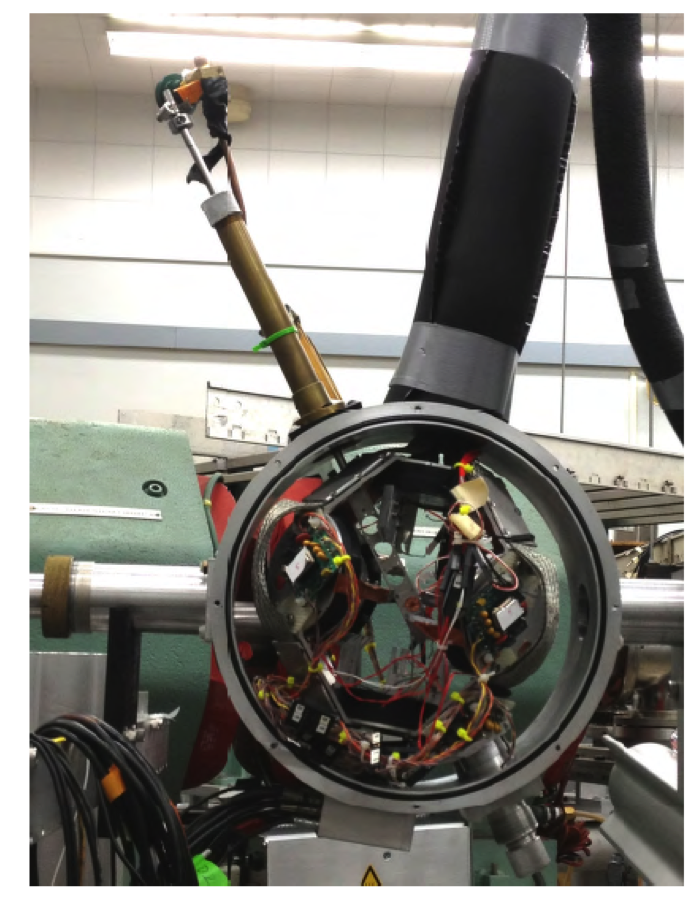
\includegraphics[scale=0.8]{Setup_Figs/Open_ICEBall.png}  
    \caption{Image of ICEBall, open for servicing. The beam would go from left to right in the picture. The target ladder is blank, in the center of ICEBall.}
    \label{fig:open_iceball}
\end{figure}

The Si(Li) detectors inside of ICEBall are 5 mm thick, with a surface area of 750 mm$^2$ \citep{metlay93:_iceball_comm}. Table \ref{tab:ICE_Det_Loc} summarizes the locations of the six Si(Li) detectors inside of ICEBall, using spherical coordinates. A thin aluminized mylar foil is placed in front of the Si(Li) detectors to block low-energy electrons and $\delta$-rays that successfully make it past the mini-orange filter (discussed in \ref{sec:mini_orange}).

\begin{table}[tpb]
    \centering
    \caption{ICEBall Detector Locations}
        \label{tab:ICE_Det_Loc}
    \begin{tabular}{c|c|c} \toprule
         Detector & $\theta$ & $\phi$  \\
         \hline
         1 & 90 & 79.2 \\ 
         2 & 270 & 100.8\\
         3 & 172 & 129.9\\
         4 & 198 & 31.7\\
         5 & 18 & 148.3\\
         6 & 355 & 50.1\\ \bottomrule
    \end{tabular}
    \\[2pt]
    \footnotesize
    The beam axis is the z-axis. $\theta$ is the angle in the xy-plane, where 0 degrees is beam left. $\phi$ is the azimuthal angle, with respect to the beam axis. All values are in degrees.
\end{table}

\subsubsection{Mini-Orange Spectrometer}
\label{sec:mini_orange}

Between the detectors and the target are mini-orange filters. First designed in the 1970s, mini-orange filters are a permanent magnet array surrounding a high-Z material, as seen in Figure \ref{fig:mini_orange} \citep{vanklinken72:mini_orange, vanklinken75:mini_orange}. In ICEBall, this material is tungsten, and the magnets are made of SmCo$_5$, and arranged in groups of 3. The tungsten acts as a blocker, lowering background from the target that can be due to $\gamma$ rays and heavy charged particles. The magnets create a field that bends electrons toward the detector, while bending positrons away from the detector, further lowering background noise. 

\begin{figure}
    \centering
    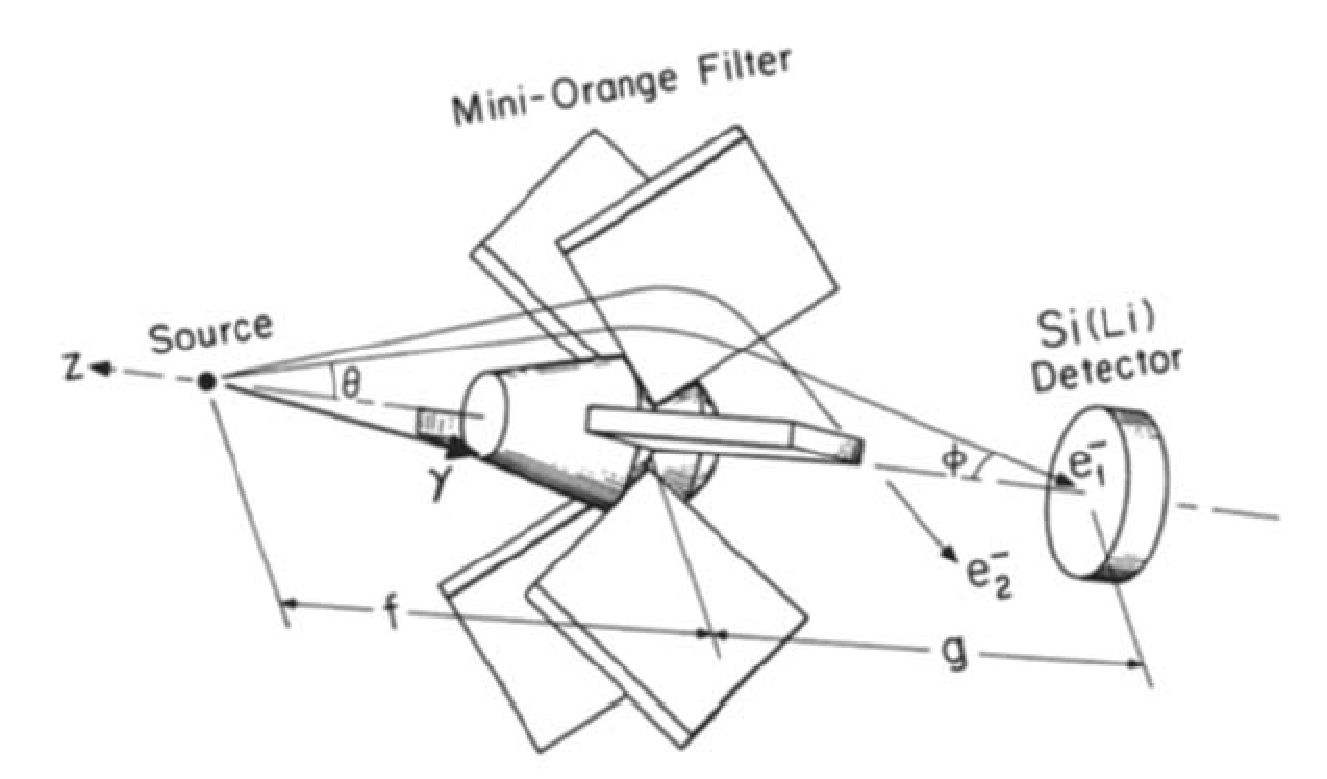
\includegraphics[scale=0.6]{Setup_Figs/mini-orange-metlay-figure.pdf}
    \caption{Graphic of the mini-orange filter. The central blocker keeps $\gamma$-rays from hitting the detector. The magnets bend electrons toward the detectors, and positrons away from the detectors. Being permanent magnets, they are optimized for a range of electron energies, and can cause overbending or underbending of electrons outside of that energy range, making the magnetic filter a factor in the efficiency. Taken from \citep{metlay93:_iceball_comm}}
    \label{fig:mini_orange}
\end{figure}

Compared to conventional spectrometers that sweep over electron energies by changing the magnetic field of the spectrometer, the mini-orange spectrometers are able to cover a wide range of energies at once. A drawback of this is the permanent magnets. The field is optimized for a range of energies, and must be pre-selected before the experiment. Switching magnets mid-experiment is not feasible, due to the downtime needed to warm-up the system, bring it to atmosphere, replace the filter, and then return the system to data taking conditions. Additionally, the efficiency of the system is a convolution of the detector's efficiency and the mini-orange filter in front of it, meaning each configuration must have a separate efficiency measurement. Tables \ref{tab:ICE_Magnet_G} and \ref{tab:ICE_Magnet_C} summarize the magnetic configurations of the mini-orange filters used in the experiments. The higher the magnetic strengths, the higher energy the peak efficiency of the mini-orange spectrometer, seen in Figure \ref{fig:filtercomp}. For the GEORGINA configuration, the magnetic strengths were all of similar values. For the Clovershare configuration, the filters were replaced on three detectors to enhance electron efficiency at higher energies.

\begin{figure}
    \centering
    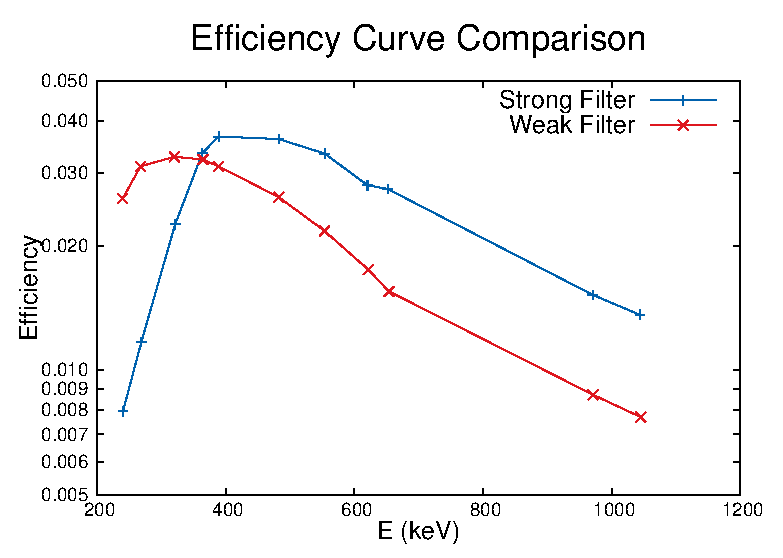
\includegraphics[scale=1]{Setup_Figs/FilterComparison.eps}
    \caption{An efficiency comparison of magnetic filters of two different strengths. The weak filter has been weakened by 70\% compared to the strong filter, using the Pitt split-pole spectrograph. Data from \citep{metlay92:_iceball_comm}.}
    \label{fig:filtercomp}
\end{figure}

\begin{table}[]
    \centering
    \caption{ICEBall magnetic strengths with GEORGINA}
     \label{tab:ICE_Magnet_G}
    \begin{tabular}{c|c|c} \toprule
         Detector & Filter & Strengths \\
         \hline
         1 & M13 & 815,740,830 \\ 
         2 & M15 & 939,911,949\\
         3 & M21 & 850,875,900 \\
         4 & M14 & 972,911,992\\
         5 & M18 & 856,913,963\\
         6 & M22 & 845,900,900\\ \bottomrule
    \end{tabular}
    \\[2]
    \footnotesize
    Magnetic strengths of the mini-orange filters used in the GEORGINA experiments, listed in Gauss. All the magnetic strengths are similar and geared for efficiency peaking at approximately 300-400 keV.
\end{table}

\begin{table}[]
    \centering
    \caption{ICEBall magnetic strengths with Clovershare}
     \label{tab:ICE_Magnet_C}
    \begin{tabular}{c|c|c} \toprule
         Detector & Filter & Strengths \\
         \hline
         1 & M13 & 815,740,830 \\ 
         2 & M20 & 1228,1292,1265\\
         3 & M21 & 850,875,900 \\
         4 & M2 & 1411,1420,1410\\
         5 & M16 & 1286,1340,1285\\
         6 & M22 & 845,900,900\\ \bottomrule
    \end{tabular}
    \\[2]
    \footnotesize
    Magnetic strengths of the mini-orange filters used in the Clovershare experiments, listed in Gauss. The magnetic strengths are mid-energy range and high-energy range for efficiency.
\end{table}

\subsection{Calibration}

ICEBall is energy and efficiency calibrated using two sources: $^{133}$Ba and $^{207}$Bi. The specific properties of the two sources are listed in Table \ref{tab:ICE_Cal_Source}. The $^{207}$Bi covers the high-energy regime, with lines around 500 keV and 1000 keV. The $^{133}$Ba covered energies from 200 to 400 keV. Both sources are low activity, preventing incomplete or overlapping charge collection from hindering the resolution of the detectors during calibration runs. 

\begin{table}[]
    \centering
    \caption{ICEBall calibration sources}
        \label{tab:ICE_Cal_Source}
    \begin{tabular}{c|c|c|c|c} \toprule
         Source & Date Measured & Activity & Energy (keV) & Intensity (\%)\\
          \hline 
         $^{133}$Ba & May-4-2012 & 0.331(7) $\mu$Ci & 240.413 & 0.331 \\
         & & & 266.868 & 0.698 \\
         & & & 320.032 & 1.308 \\
         & & & 347.866 & 0.370 \\
         \hline
         $^{207}$Bi & May-4-2012 & 0.306(8) $\mu$Ci & 481.697 & 1.562 \\ 
         & & & 554.4 & 0.469 \\
         & & & 975.657 & 7.243 \\
         & & & 1048.1 & 1.838 \\\bottomrule
    \end{tabular}
    \\[2]
    \footnotesize
    Calibration source information for ICEBall. The energies and the respective intensities are listed for each source. Intensities are taken from \cite{trzaska90:_calibration}. The intensity of the 347 keV line in $^{133}$Ba is both the 384K and 356L intensities combined.
\end{table}

The energy calibration is assumed to be quadratic in nature, although both linear and quadratic calibrations are performed. Figure \ref{fig:iceball_cal} shows both of these fits and their respective residuals for one of the Si(Li) detectors. These values are summarized in the next chapter for each experiment.

\begin{figure}
    \centering
    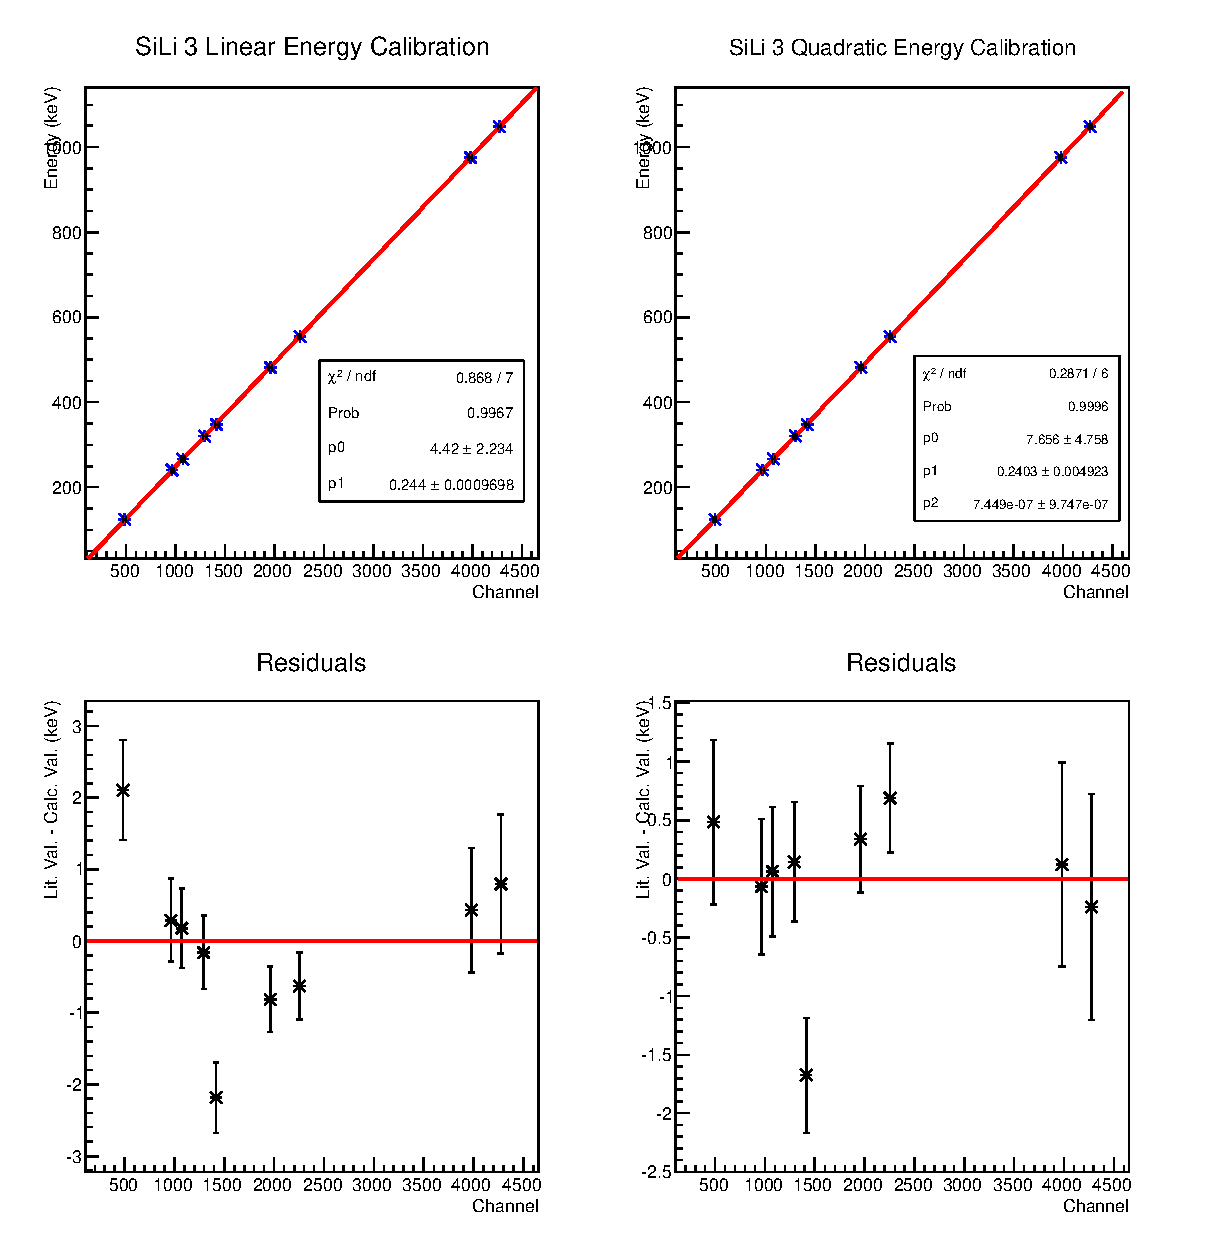
\includegraphics[scale=0.75]{Setup_Figs/sili_3.eps}
    \caption{Linear and quadratic energy calibrations of one Si(Li) detector, using the electron energies listed in Table \ref{tab:ICE_Cal_Source}. The top graphs show the calibrations, while the graphs beneath show the respective residuals. The calibration is in much better agreement in the quadratic fit, as seen in the residuals.}
    \label{fig:iceball_cal}
\end{figure}

The efficiency calibration is fitted to equation

\begin{equation}
    ln(\epsilon) = p_1+p_2ln(E)+p_3E
    \label{eq:SiLi_Eff}
\end{equation}

The efficiency is a convolution of the magnetic configuration and the inherent detector efficiency. Using the efficiency points, the analytic expression for the efficiency was determined empirically in previous work \citep{battaglia15:_iceball_176lu}. These experimental values are summarized in the next chapter for each experiment.

\section{Gamma Detection}

Gamma radiation is highly penetrating, making semiconductor detectors of normal purity unusable, as they have limitations on the depth of the depletion region that are nowhere near the necessary depths needed for fully stopping gamma radiation. The depletion depth is inversely proportional to the number of impurities in the material \citep{knoll00:rad_det_meas}. High-purity germanium, also known as intrinsic germanium, detectors decrease these impurities to increase the depletion depth, resulting in depths of several centimeters.

Like other semi-conductor detectors, there are dead zones that attenuate the radiation. Generally, this attenuation is negligible above 200 keV. These detectors have a high resolution due to the small bandgap of 0.7 eV in germanium. This small bandgap comes at a price, and HPGe detectors can only be operated at liquid nitrogen temperatures, as putting any voltage on a room temperature HPGe would result in high leakage currents and noise, making detection impossible.

\subsection{GEORGINA}

GEORGINA is a compact array of high-purity germanium (HPGe) detectors for $\gamma$-ray experiments\citep{isnap18:_georgina}. The detectors are 100\% relative efficiency (as compared with a $3"\times3"$ NaI detector at 1332 keV). These detectors were designed for use with low cross-section astrophysical capture reactions, meant to cover a large solid angle. There are a total of five detectors. The detectors were designed with the crystal at a $90^{\circ}$ from the cold-finger, as seen in Figure \ref{fig:georgina}.

\begin{figure}
    \centering
    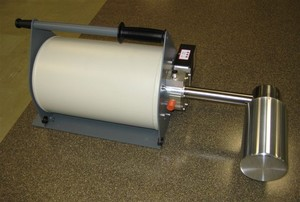
\includegraphics{Setup_Figs/georgina_example.png}
    \caption{An example of one of the GEORGINA detectors. The crystal is at a $90^{\circ}$ from the cold finger, allowing the long side of the crystal to be placed next to the target, to optimize solid angle coverage. In the experiment, the circular face of the crystal was placed toward the target.}
    \label{fig:georgina}
\end{figure}

One of the two detectors had Bismuth Germanate (BGO) detectors from Argonne National Laboratory around it to cut down on background from incomplete charge collection, these can be seen in Figure \ref{fig:georgina_config}. BGO detectors have a high efficiency, but poor resolution, and are good to use as a veto system. In the event that a gamma-ray does not deposit its full energy in the HPGe crystal, the BGO detectors surrounding the crystal should pick up the remaining energy. This indicates the event was incomplete in energy and should be excluded from the data. This is a manual cut made during the analysis procedure by looking at the data from the BGO detectors.

\subsection{CloverShare}

CloverShare is a group of nine HPGe clover detectors with BGO shields, that originated at Yale University as part of the YRAST Ball array \citep{beausang00:_yrast}. They were sent to various laboratories and universities for series of experiments, including the NSL. Two campaigns of experiments were run with CloverShare, each one involving an ICEBall experiment.

The CloverShare detectors are large, segmented HPGe detectors, with fitted BGO shields, seen in Figure \ref{fig:clover_example}. Each detector is segmented into four crystals, resembling a clover. Due to the "add-back" capability of these detectors, summing over the close-proximity crystals, the detectors each have a total relative efficiency \~150\%, whereas each individual crystal is approximately 20\% efficient. In the first of the two experiments, 7 detectors were used. In the second, 5 were used, as two experienced pre-amplifier problems during the previous campaign. The detectors used biases between -3000 and -4000 V, and were kept cold using a liquid nitrogen autofill system.

\begin{figure}
    \centering
    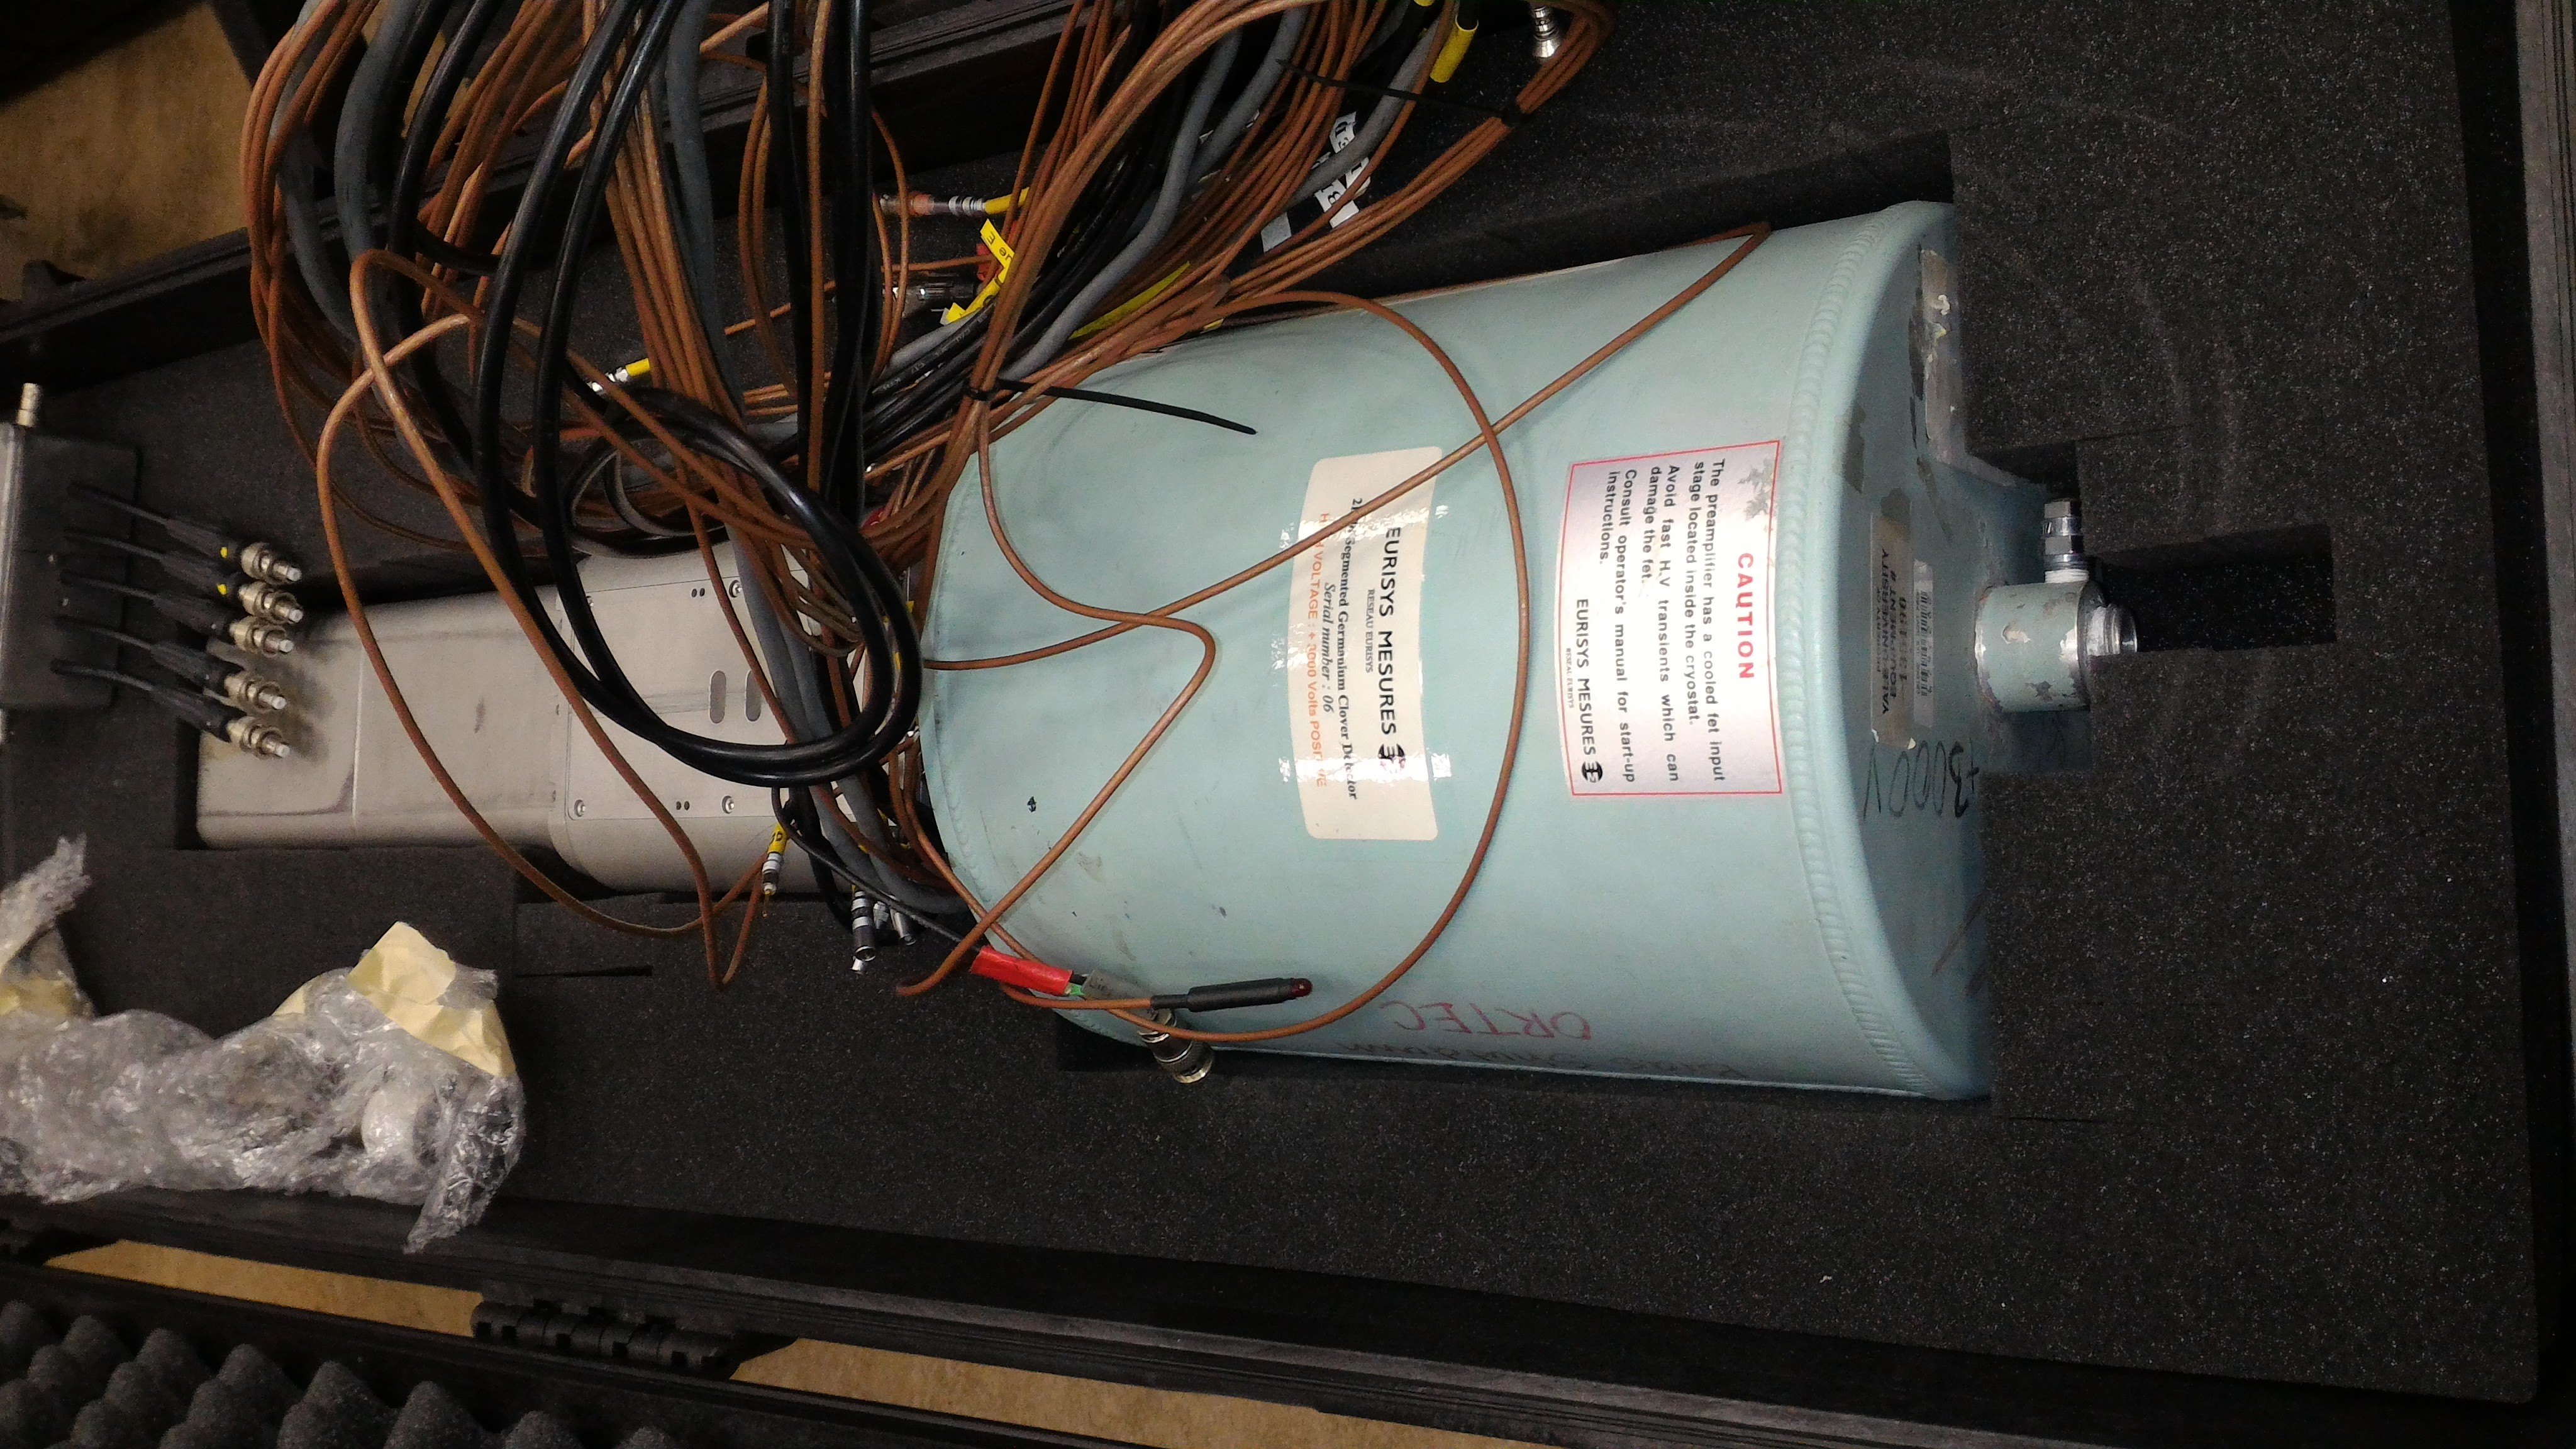
\includegraphics[scale=0.1]{Setup_Figs/P_20160118_094821.jpg}
    \caption{Example of one of the Clovershare detectors.}
    \label{fig:clover_example}
\end{figure}

\subsection{Calibration}
\label{sec:clover_cal}

Both sets of detectors were calibrated using a $^{152}$Eu source, in addition to the ICEBall sources. The information about the sources is in Table \ref{tab:GEORGINA_Cal_Source}. The $^{152}$Eu source was not designed to sit perfectly on the target ladder, while the two ICEBall sources were. So, even though the Eu source was attached to the target ladder for calibration, using it as a measure of absolute efficiency was not possible. To use the $^{152}$Eu for efficiency, a linear extrapolation of the efficiency of the 344 keV line was done using the 303 keV and 356 keV lines in $^{133}$Ba. All points in the Eu were then scaled based on this. Additionally, several background lines could be used to extend the energy calibration up to 2700 keV. The energy calibration was fit to a polynomial, and fits up to the fifth order were done to find the best calibration without overfitting. For examples of these fits, see the next chapter.

\begin{table}[]
    \centering
    \small
    \caption{GEORGINA calibration sources}
    \begin{tabular}{c|c|c|c|c} \toprule
         Source & Date Measured & Activity & Energy (keV) & Intensity (\%)\\
          \hline 
         $^{133}$Ba & May-4-2012 & 0.331(7) $\mu$Ci & 80.997 & 0.3406 \\
         & & & 276.398 & 7.164 \\
         & & & 302.853 & 18.33 \\
         & & & 356.017 & 62.05 \\
         & & & 383.851 & 8.94 \\
         \hline
         $^{207}$Bi & May-4-2012 & 0.306(8) $\mu$Ci & 569.702 & 97.75 \\ 
         & & & 1063.662 & 74.09 \\
         \hline
         $^{152}$Eu & & & 121.7825 & 28.65 \\
         & & & 244.6989 & 7.582 \\
         & & & 344.281 & 26.6 \\
         & & & 411.115 & 2.262 \\
         & & & 443.965 & 3.125 \\
         & & & 778.903 & 13.017 \\
         & & & 867.39 & 4.26 \\
         & & & 964.055 & 14.758 \\
         & & & 1085.842 & 10.062 \\
         & & & 1089.7 & 1.738 \\
         & & & 1112.087 & 13.587 \\
         & & & 1408.022 & 20.945 \\\bottomrule
    \end{tabular}
    \footnotesize
    \item Calibration source information for GEORGINA. The energies and the respective intensities are listed for each source. Intensities are taken from \cite{trzaska90:_calibration}. The  $^{152}$Eu does not have activity and intensity, as it was normalized to the $^{133}$Ba.
    \label{tab:GEORGINA_Cal_Source}
\end{table}

The $^{152}$Eu source was placed on the individual detectors instead of centered in the trap, as it does not mount well to the target ladder. To use the $^{152}$Eu for efficiency, a linear extrapolation of the efficiency of the 344 keV line was done using the 303 keV and 356 keV lines in $^{133}$Ba. All points in the Eu were then scaled based on this. A characteristic fit of the efficiency of these detectors can be seen in Figure \ref{fig:clover_eff}.

The efficiency calibration is fitted to equation

\begin{equation}
    ln(\epsilon) = a_0-(a_1+a_2\times e^{-a_3\times E})\times E^{-a_4\times E}\times ln(E)
    \label{eq:Ge_Eff}
\end{equation}

A characteristic fit can be seen in Figure \ref{fig:clover_eff}. The CloverShare detectors were also calibrated using a $^{56}$Co source that was created on the FN accelerator days before the experiment. The information about the source is in Table \ref{tab:Co_Energy}. 

\begin{table}[t]
    \centering
    \caption{$^{56}$Co Calibration Information}
    \label{tab:Co_Energy}
    \begin{threeparttable}
    \begin{tabular}{c|c}
    \toprule
         Activity & $\gamma$ Energy (keV)  \\ \hline
         6.44 $\mu$Ci\tnote{a} & 846.77 \\
         & 977.372 \\
         & 1037.843 \\
         & 1175.101 \\
         & 1238.288 \\
         & 1360.212 \\
         & 1771.357 \\
         & 2015.215 \\
         & 2034.791 \\
         & 2598.5 \\
         \bottomrule
    \end{tabular}
    \begin{tablenotes}[para]
    Energies used in $^{56}$Co for calibration, as well as activity.
    \newline\item[a] Measured on Mar-16-2016
    \end{tablenotes} 
\end{threeparttable}
\end{table}

\begin{figure}[t]
    \centering
    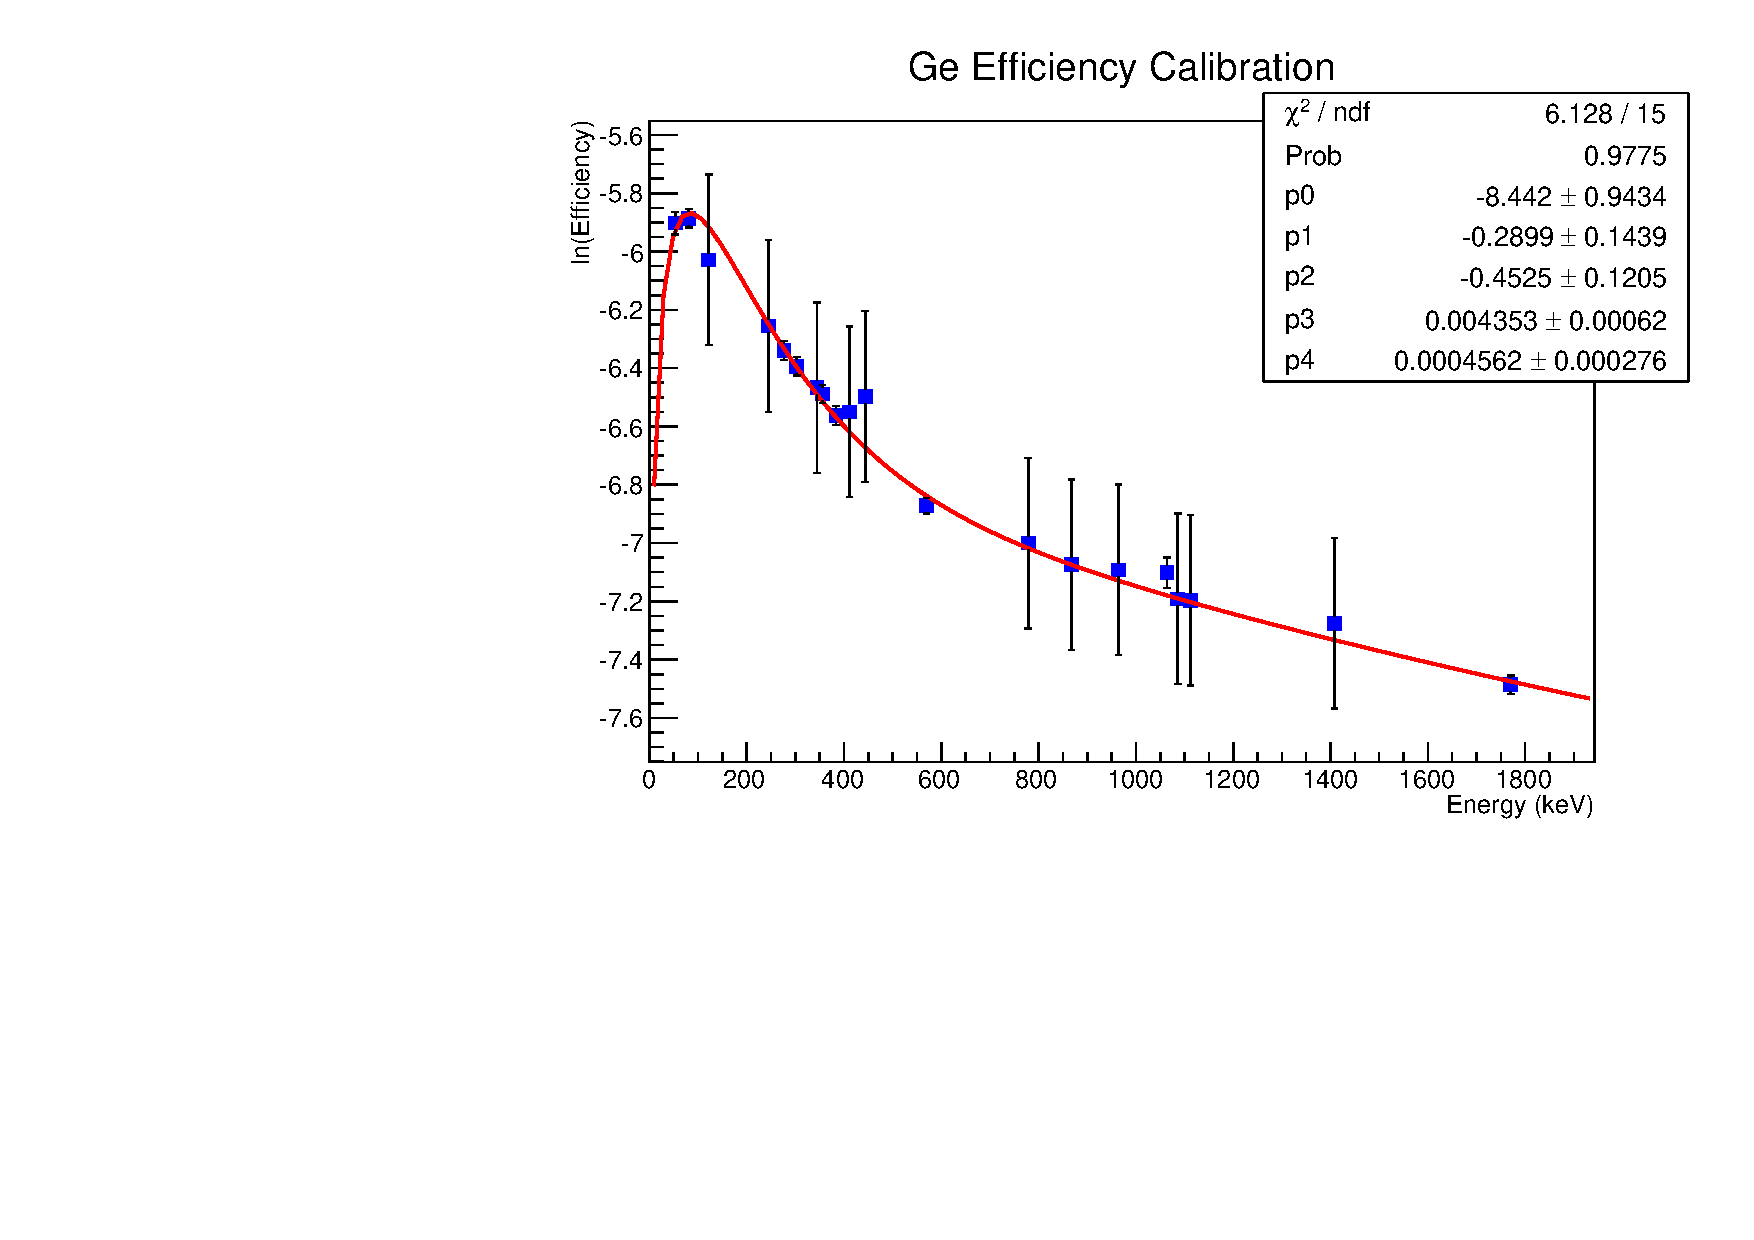
\includegraphics[scale=0.7]{Setup_Figs/Clover1_Eff_05232017.pdf}
    \caption{A characteristic fit of the Clovershare detector efficiencies. The points with large error bars are the $^{152}$Eu points, as the scaling of the points caused a large uncertainty, compared to the $^{207}$Bi and $^{133}$Ba.}
    \label{fig:clover_eff}
\end{figure}

As the clovers are comprised of four separate crystals, the efficiency was taken for the individual leaves, and once the detectors had been calibrated, they were summed together. Figure \ref{fig:Clover_ind_vs_sum} shows the comparison. As is expected, there is a small improvement in the higher energies. This is due to the summation of otherwise incomplete charge collection due to compton scattering within individual crystals. This did cause the efficiency at lower energies to appear lower, but this is due to the summing of cascades of energies over the segments. The summed crystals were used for analysis, and will be used in spectra from here on forward.

\begin{figure}[hbt!]
    \centering
    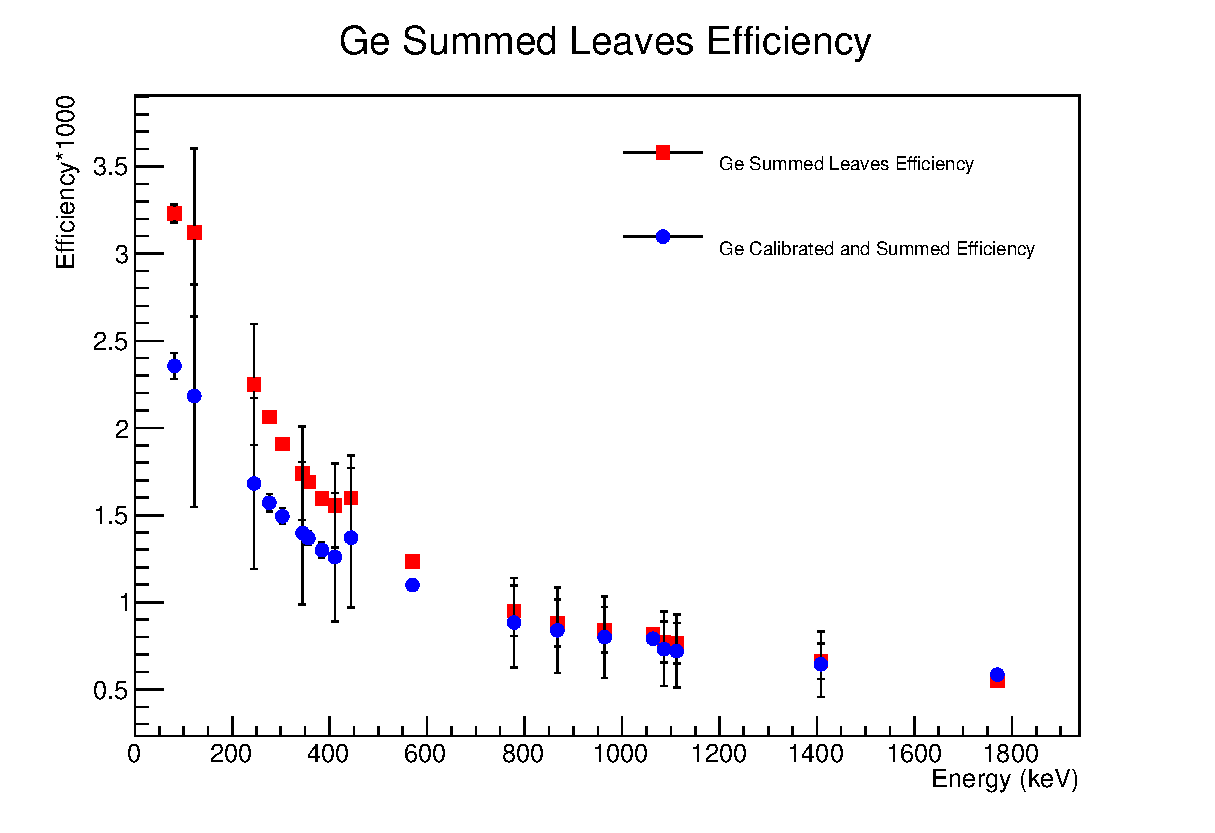
\includegraphics[scale=0.7]{Setup_Figs/Efficiency_ind_vs_sum.eps}
    \caption{Efficiency of a CloverShare detector, with the individual leaves' efficiency summed together, compared to the efficiency of the leaves calibrated and summed together. The different colors/shapes indicate the different sources, as labeled.}
    \label{fig:Clover_ind_vs_sum}
\end{figure}

Each leaf of the clovers was energy calibrated. An unusual trend in the residuals was found in all cases, as seen in Figure \ref{fig:Clover_ene_res}. This trend could not be corrected for by using a higher-order polynomial, as is usually the case for integral non-linearities in multi-channel analyzers \citep{knoll00:rad_det_meas}. Instead, this appears to be a differential non-linearity in the electronics, resulting in discontinuities. As will be discussed in the next section, the electronics used for the experiment are not primarily used with detectors of this sensitivity.

\begin{figure}
    \centering
    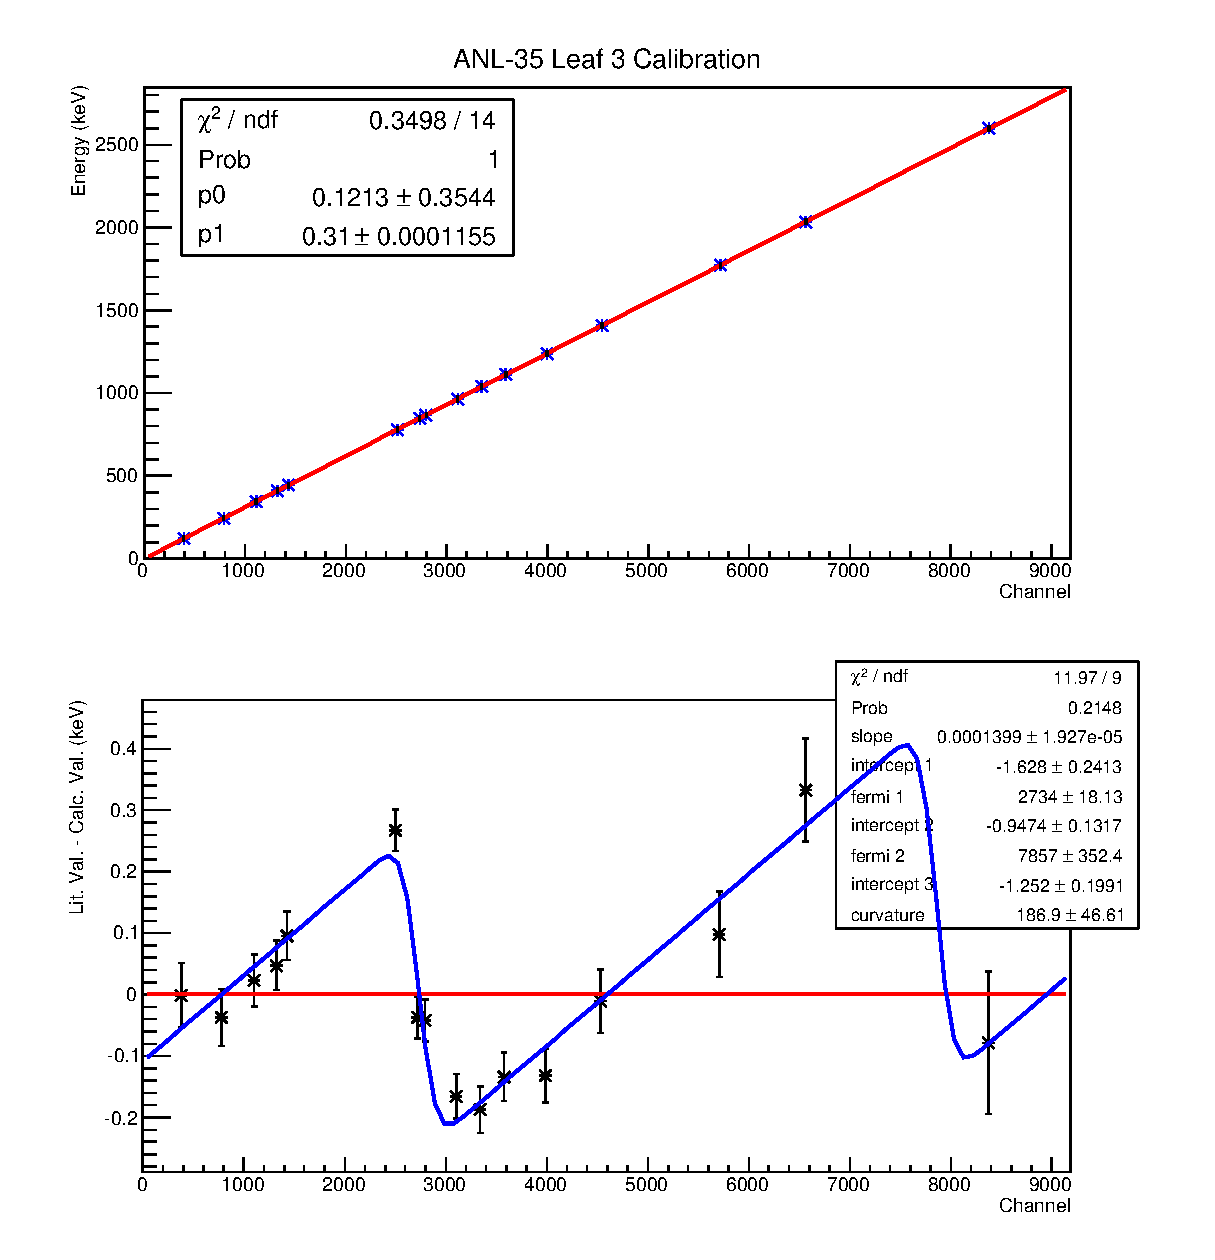
\includegraphics[scale=0.7]{Setup_Figs/Clover_res_cal.eps}
    \caption{A look at the energy calibration of an individual leaf in an HPGe Clover detector. The upper graph is a linear calibration. The lower graph is a look at the residuals. For HPGe detectors, $\pm0.4$ keV is not a good energy calibration. Here, the sawtooth fit that was derived from the differential non-linearity in the electronics is seen fitted to the data.}
    \label{fig:Clover_ene_res}
\end{figure}

\section{Target Fabrication}

Electrons must escape the target for detection. All materials have some stopping power for radiation, based on the material, thickness, and type of particle. The Beta-Bloch formula can be used to calculate this stopping power, with several programs, including SRIM, created to make and tabulate these values\citep{ziegler10:_srim}. A thicker target causes energy loss and straggling effects, blurring out the conversion electron spectrum, meaning a thinner target is a more ideal situation.

Enriched, self-supporting samarium targets were used for this experiment. Table \ref{tab:target} has the enrichment and thickness of the targets used. The material started as Sm$_2$O$_3$. Using the reaction

\begin{equation}
    Sm_2O_3 + Hf \xrightarrow{} HfO_2 + Sm
    \label{eq:sm_hf}
\end{equation}

at a temperature of 1520-1820 K the samarium was extracted as a metal \citep{clifford02:_target}. Once cooled, it was rolled as thin as possible. Samarium easily oxidizes, stagnating the rolling process, as too much work on the material at once could cause instantaneous oxidization, resulting in the loss of the target. Rolling had to be done incrementally, giving the material time to rest.

\begin{table}[]
    \centering
    \caption{Target Enrichment and Thickness}
    \begin{tabular}{c|c|c}
    \toprule
         Isotope & Enrichment (\%) & Thickness (mg/cm$^2$) \\
         \hline
         $^{152}$Sm & $>98$ & 1.44  \\ 
         $^{154}$Sm & $>98$ & 1.7 \\ 
         \bottomrule
    \end{tabular}
    \label{tab:target}
\end{table}

\section{Experimental Configuration and Operation}

\subsection{Experimental Beam Operation}

The experiments with GEORGINA were done using a bunched beam, creating a set timing signal to help with coincidence. The beam was bunched before the accelerator, with a time separation of 600 ns between bunches and a full-width half-maximum of 16 ns for the bunch. The timing of these bunches is shown in Figure \ref{fig:bunched}. Clear separation in of the bunches is visible. The accelerator was run with a terminal voltage of 6.64 MV, with $^{4}$He$^{2+}$ being sent through the machine, resulting in a beam of energy 20 MeV, including the initial 60 kV kick from the HIS. 

\begin{figure}
    \centering
    \includegraphics[scale=0.7]{Setup_Figs/Time-of-Flight.eps}
    \caption{This is a plot of the HPGe 1 detector time minus the buncher time. Two distinct peaks can be seen in the spectrum, the main timing peak close to 0, and the much smaller secondary peak, coming from a second bunching signal. The bunching signal only acts as a stop signal for the timing. It can also be used as a veto, as events without a valid buncher time are not real, or are background.}
    \label{fig:bunched}
\end{figure}

\subsection{GEORGINA Configuration and Electronics}
\label{sec:GEORGINA_electronics}

While the GEORGINA detectors were designed for large efficiency up to 12 MeV, they were used in this experiment for energies up to 4 MeV. Two GEORGINA detectors were used in the experiment with ICEBall. The location of the detectors is given in Table \ref{tab:GEORGE_Det_Loc}. They were placed with the face of the detector against ICEBall.

\begin{table}[]
    \centering
    \caption{GEORGINA Detector Locations}
    \label{tab:GEORGE_Det_Loc}
    \begin{tabular}{c|c|c} \toprule
         Detector & $\theta$ & $\phi$  \\
         \hline
         1 & 0 & 90 \\ 
         2 & 180 & 90\\ \bottomrule
    \end{tabular}
    \\[2pt]
    \footnotesize
    The beam axis is the z-axis. $\theta$ is the angle in the xy-plane, where 0 degrees is beam left. $\phi$ is the azimuthal angle, with respect to the beam axis. All values are in degrees.
\end{table}

The ICEBall-GEORGINA pairing can be seen in Figure \ref{fig:georgina_config}. The data taken with this pairing of detectors used the electronics set-up from previous experiments\citep{battaglia15:_iceball_176lu}. Signals from the Si(Li), HPGe, and BGO detectors were split into two signals, one for timing and one for energy, as seen in Figure \ref{fig:iceball_electronics}. For the Si(Li) and HPGe, the energy signals are run through an amplifier NIM (Nuclear Instrumentation Modules) before being fed into the Mesytec analog-to-digital converter (MADC-32) VME (Versa Module Europa) bus module for analog-to-digital conversion \citep{mesytec:_ADC}. This module has 13 bit resolution. The timing signals went through a Timing Filter Amplifier (TFA) NIM and a Constant Fraction Discriminator (CFD) NIM to clean the signal before being converted using a Caen V775 time-to-digital converter (TDC) module, with 12 bit resolution\citep{caen:_TDC}. The TFA module shapes the pulse signal and amplifies it. The CFD module allows for triggering on the same part of the slope of a signal, regardless of the height of the signal, giving more consistent timing. A third module, the Caen V830 32 Channel Latching Scaler, was used to keep track of detector rates for deadtime, beam current, and trigger rates\citep{caen:_scaler} via a second signal sent from the CFD module. Logic was done using a third signal from the CFD module and logic NIM modules that employ an emitter-couple logic circuit. These can be adjusted for either "and" or "or" logic. This logic created the trigger that acted as the start signal.The data structures of the events in these modules are explicitly written in Tables \ref{tab:word_MADC}, \ref{tab:word_CAEN}, \ref{tab:word_V830}.

\begin{figure}[hbt!]
    \centering
    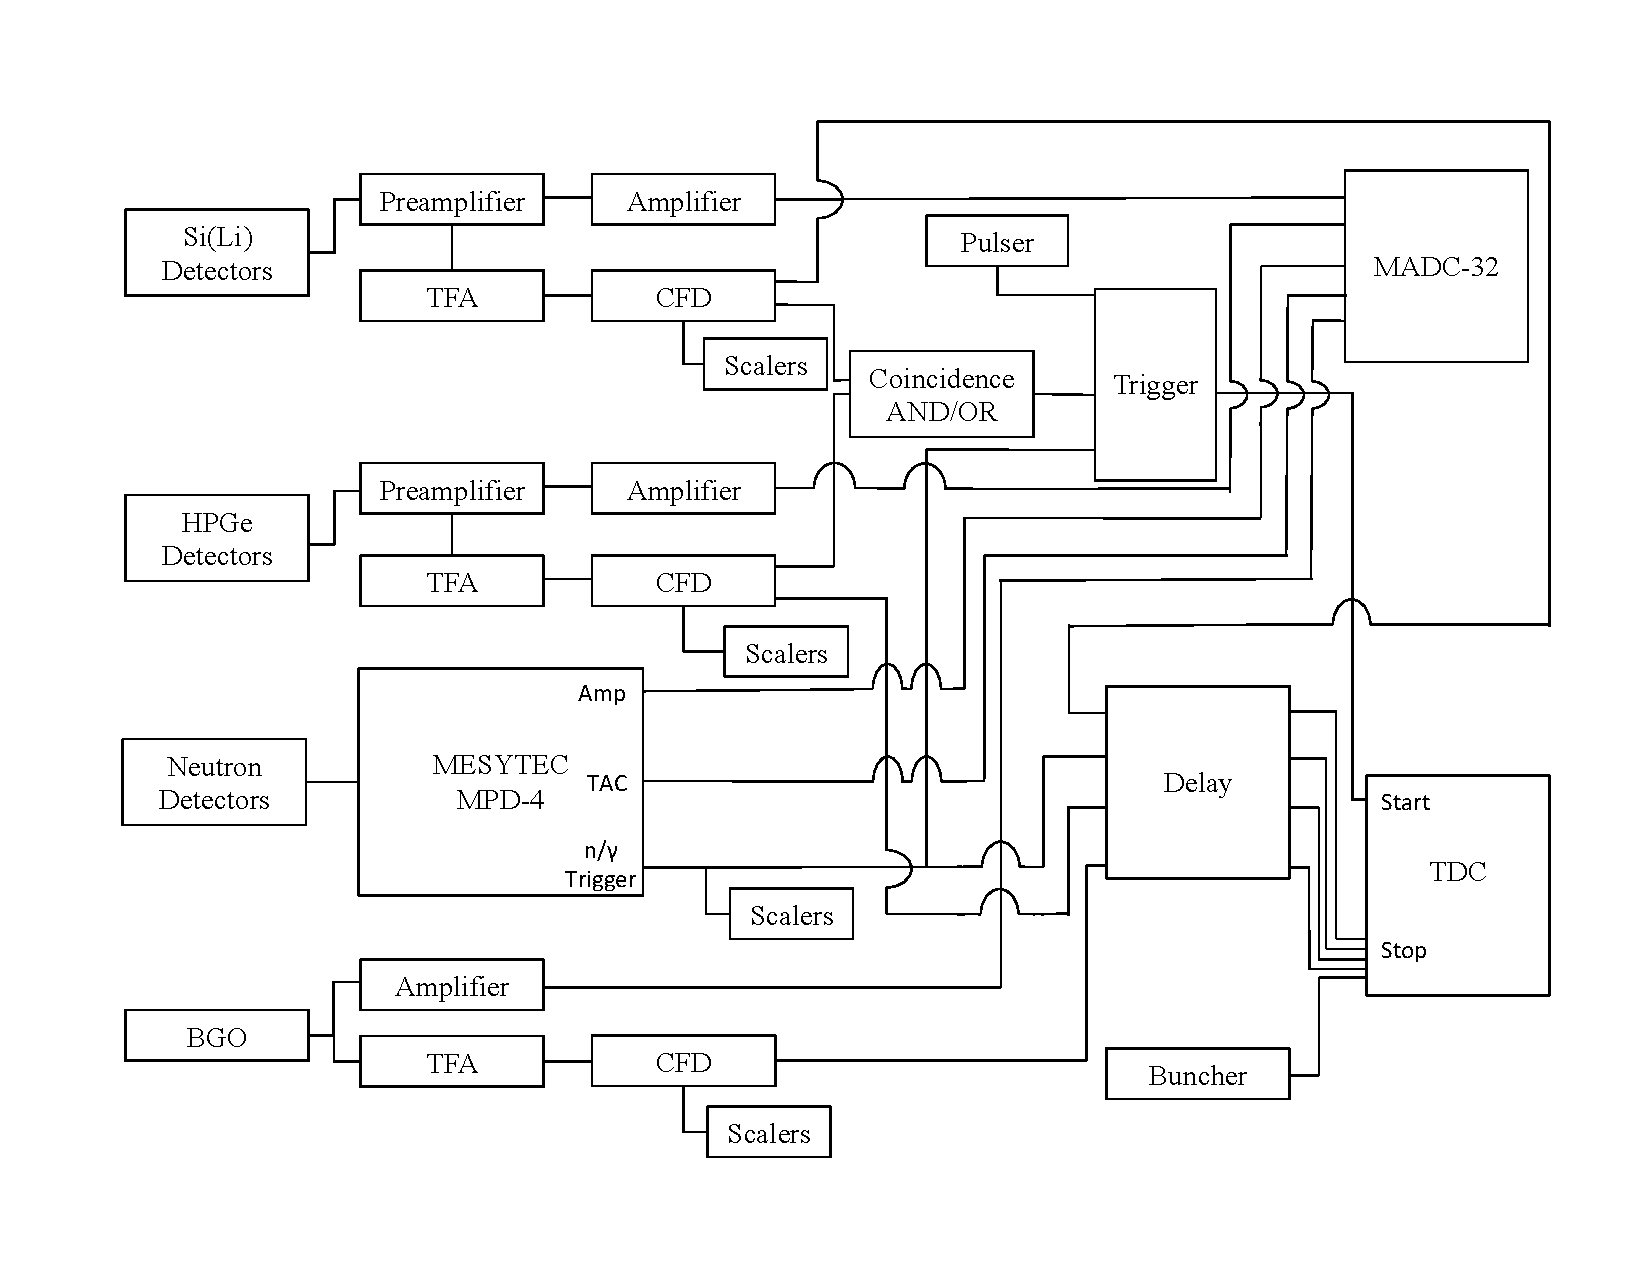
\includegraphics[scale=0.5]{Setup_Figs/electronics-diagram.pdf}
    \caption{A schematic of the electronics for the ICEBall-Georgina set up. See section \ref{sec:GEORGINA_electronics} for a detailed explanation. Taken from \citep{battaglia15:_iceball_176lu}.}
    \label{fig:iceball_electronics}
\end{figure}

The BGO detectors went through an amplifier before being fed directly into the MADC-32. Both the Si(Li)s and the HPGe detectors went into a preamplifier before going into an amplifier, and then the MADC-32. The amplifier allowed for the adjustment of the gain, to optimize the energy regime of interest. The timing signals were sent through a TFA before going through a CFD and being delayed and sent as timing stop signals, as well as being recorded into the scalers. The stop signal was delayed by \~500ns to prevent self-triggering. Start timing signals were put into a logic coincidence for the trigger. The trigger could be adjusted if the count rate were too high, but the ideal case was the "OR" coincidence, where a Si(Li) or HPGe detector could trigger the start. When this occurred, the signal was sent to a trigger, which sent the TDC a start signal. Stop signals could come from any of the three types of detectors, or the bunched beam being used.

The data was collected from the VME modules using the Michigan State University NSCL data acquisition system (DAQ)\citep{nscl:_daq}. The data file, known as an event or "evt" file, is only compatible with the analysis software SpecTcl\citep{nscl:_daq}. For online analysis, SpecTcl was used. However, for the purposes of gating and fitting, it is inadequate. These evt files were instead converted into "root" files, for use with the CERN Root Data Analysis Framework\citep{brun97:_root}. This open source software is programmable through C++, allowing for a robust set of features. This conversion was done using a program called \texttt{evt2root}\citep{smith14:_evt2root}.

\subsection{Clovershare Configuration and Electronics}

Due to the fixed nature of the ICEBall detectors, the clovers were limited in the angles they could be placed at to optimize efficiency. With the tungsten blockers in front of the Si(Li) detectors to block gamma-rays and x-rays, placing the clovers behind these detectors would drastically reduce efficiency. The system was modeled in AutoDesk Inventor \citep{autodesk:_inventor} to visualize the detector placement, and find an ideal setup to optimize the HPGe detectors. Figure \ref{fig:inventor} shows the resulting model and placements, as well as several unmoveable obstructions, like cable trays, that needed to be worked around. Figure \ref{fig:clovershare_config} shows the final placements for the seven-detector configuration, in the experimental hall. Table \ref{tab:Clover_Det_Loc} lists the detector placements for the seven and five detector configurations, labeled as Experiments 1 and 2.

\begin{figure}[t]
    \centering
    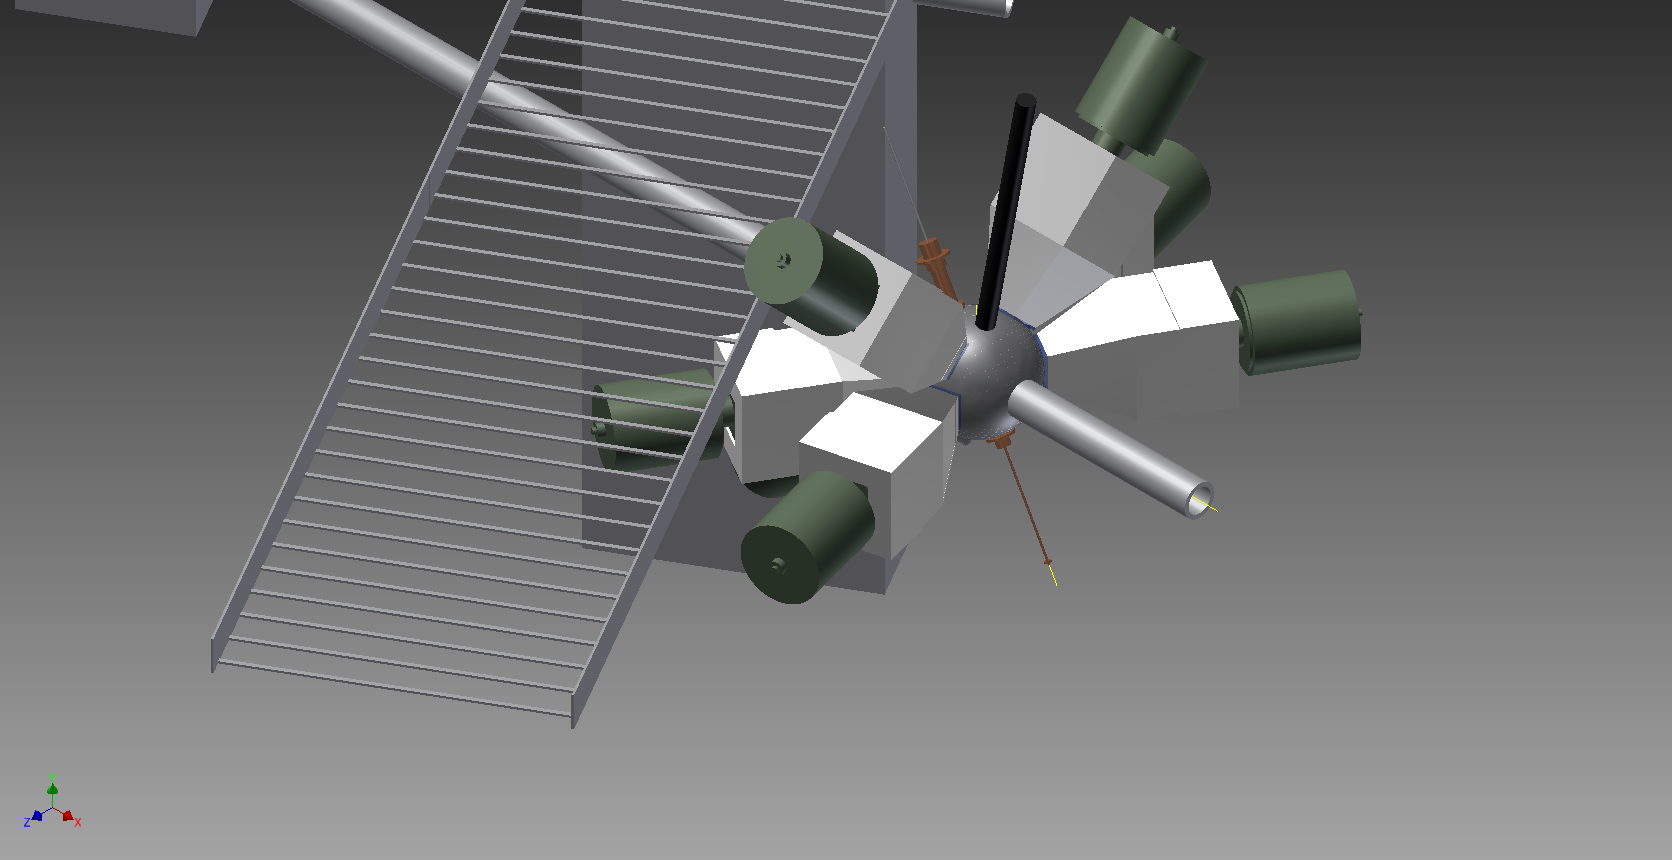
\includegraphics[scale=0.3]{Setup_Figs/FullyAssembled-50cm-newpositions-rightiso.png}
    \caption{ICEBall modeled in Autodesk Inventor \citep{autodesk:_inventor} with the Clovershare detectors placed around it in locations to optimize efficiency. Once ICEBall had been modeled, the detectors were moved around to make sure they were not behind the tungsten blockers. The beamline was also modeled to know where obstructions existed that prevent the Clovershare detectors from being place there.}
    \label{fig:inventor}
\end{figure}

\begin{table}[t]
    \centering
    \caption{Clovershare detector locations}
    \label{tab:Clover_Det_Loc}
    \begin{tabular}{c|c|c!{\vrule width 0.5mm}c|c} \toprule
        & \multicolumn{2}{c!{\vrule width 0.5mm}}{Experiment 1} & \multicolumn{2}{c}{Experiment 2} \\
        \hline
         Detector & $\theta$ & $\phi$ & $\theta$ & $\phi$ \\
         \hline
         ANL-35 & 270 & 145 & 270 & 145 \\ \hline
         LBL-7 & 0 & 111 & 0 & 111 \\ \hline
         ANL-23 & 0 & 66 & \multicolumn{2}{c}{Not Used}\\ \hline
         LBL-6 & 180 & 111 & \multicolumn{2}{c}{Not Used}\\ \hline
         LBL-10 & 180 & 66 & 180 & 71\\ \hline
         ANL-31 & 45 & 90 & 45 & 90\\  \hline
         ANL-18 & 135 & 90 & 180 & 111\\ 
         \bottomrule
    \end{tabular}
    \\[2]
    \footnotesize
    The detectors are listed by identification name. The angles for the detectors are given for both experiments run with the Clovershare detectors. ANL-23 and LBL-6 were not used in the second experiment due to preamplifier issues. The beam axis is the z-axis. $\theta$ is the angle in the xy-plane, where 0 degrees is beam left. $\phi$ is the azimuthal angle, with respect to the beam axis. All values are in degrees.
\end{table}

The electronics used for the Clovershare series of experiments were designed for use with the High Efficiency TOtal absorption spectrometeR (HECTOR), a NaI(Tl) detector array\citep{reingold19:_HECTOR}. The HECTOR data acquisition system is based on the Michigan State University NSCL digital data acquisition system (DDAS). This system uses three XIA Pixie-16 modules \citep{xia:_pixie} which are 16 channel 14-bit 100 MSPS digitizers. The data structure of this system can be seen in Table \ref{tab:word_XIA}. Signals from detectors were fed directly from the preamplifiers to the Pixie modules, which did the amplification, shaping, timing, and logic triggers within the module through adjustments on the data acquisition computer, seen in Figure \ref{fig:pixie_electronics}. In the ICEBall setup, these functions were done using the NIM electronics. NaI(Tl) detectors have far lower resolution than HPGe detectors, so the differential non-linearities are not noticeable in the HECTOR data.

\begin{figure}
    \centering
    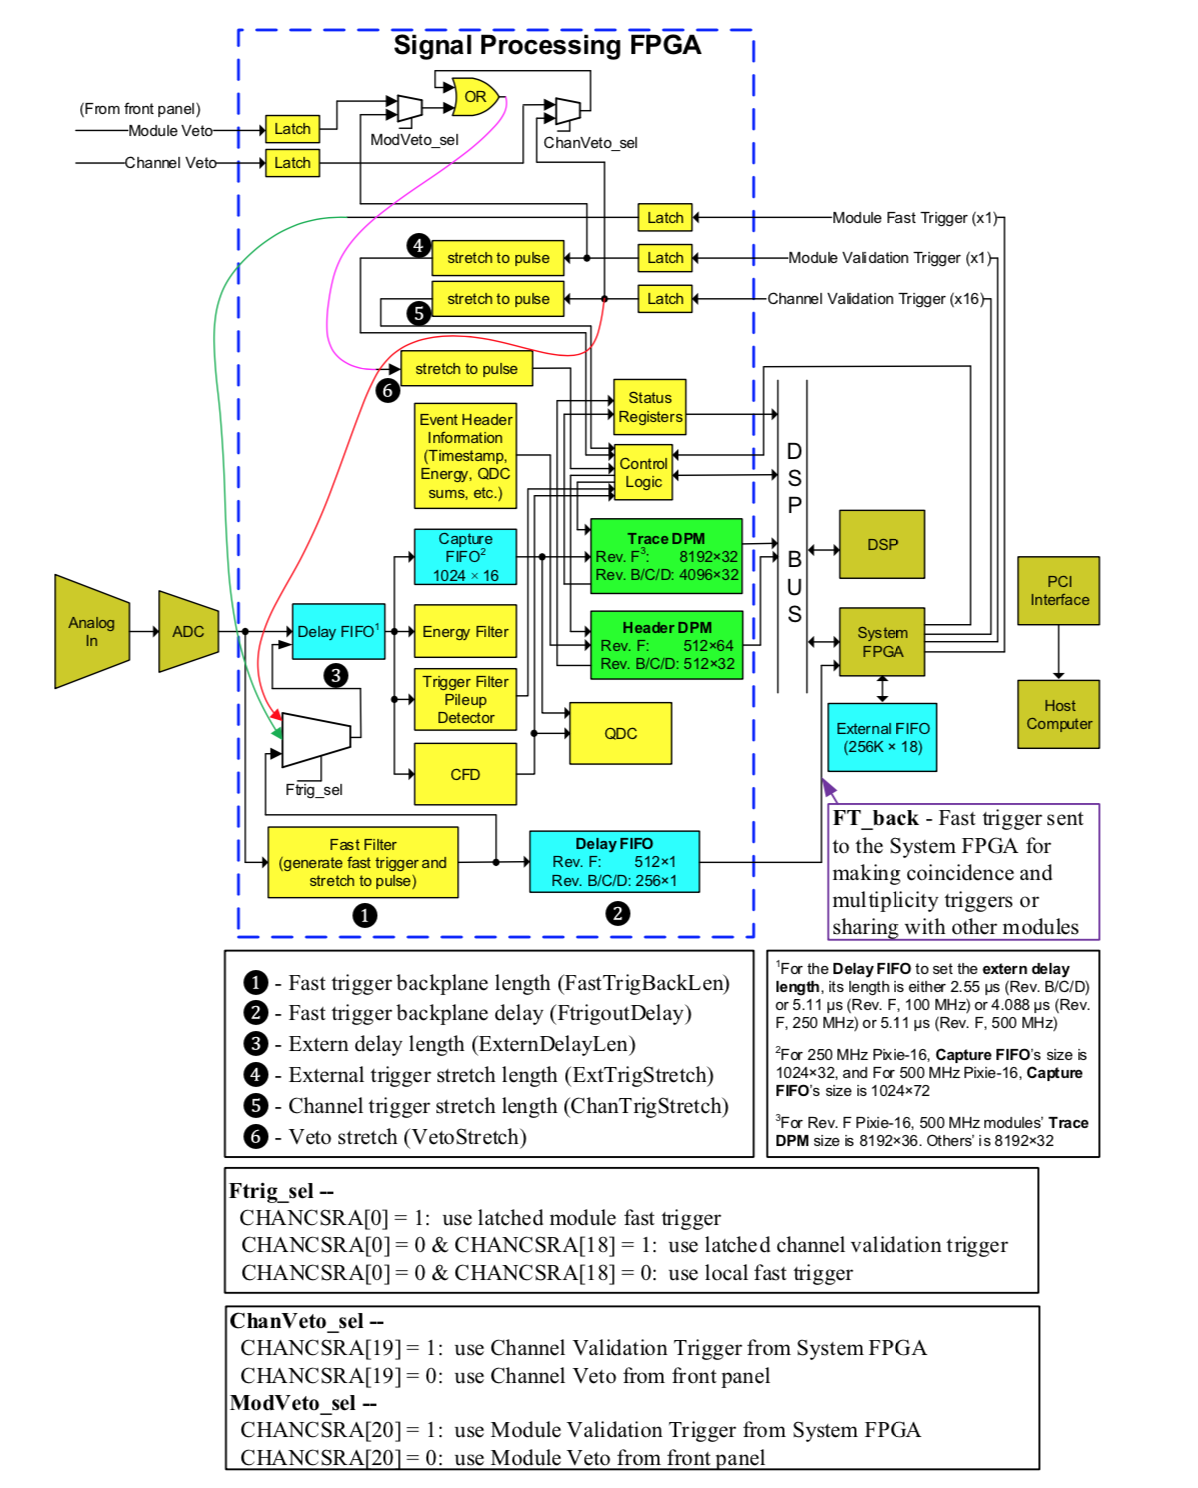
\includegraphics[scale=0.75]{Setup_Figs/pixie_electronics.png}
    \caption{The signal processing done by the XIA Pixie-16 electronics. All the processing is done within the module. Taken from \citep{xia:_pixie}.}
    \label{fig:pixie_electronics}
\end{figure}

The Pixie modules were unable to produce enough gain in the amplifier section for the Si(Li) detectors to cover a significant number of channels for resolution, so the detectors' signals were put through fast filter amplifiers \citep{ortec:_fastamp} to boost the signal before being fed into the DDAS. Fast amplifiers were used due to the fast timing and acquisition nature of the Pixie-16 modules and DDAS. 

As with the ICEBall data, these files were event files that were then converted in root files for further analysis.

\begin{landscape}
\begin{table}[]
    \centering
    \small
    \caption{\label{tab:word_MADC}Data Event - MADC32 (32 Bit Word)}
    \begin{tabular}{c|c|c|c|c|c|c|c|c|c|c|c|c|c|c|c|c|c|c|c|c|c|c|c|c|c|c|c|c|c|c|c}
 %   \begin{tabularx}{\linewidth}{X|X|X|X|X|X|X|X|X|X|X|X|X|X|X|X|X|X|X|X|X|X|X|X|X|X|X|X|X|X|X|X}
        \toprule
        \multicolumn{32}{c}{Header} \\
        \hline
        \multicolumn{2}{c|}{2} & \multicolumn{6}{|c|}{6} & \multicolumn{8}{|c|}{8} & 1 & \multicolumn{3}{|c|}{3} & \multicolumn{2}{|c|}{2} & \multicolumn{10}{|c}{10} \\
        \multicolumn{2}{c|}{header signature} & \multicolumn{6}{|c|}{subheader} & \multicolumn{8}{|c|}{module id} & output format & \multicolumn{3}{|c|}{adc resolution} & \multicolumn{2}{|c|}{} & \multicolumn{10}{|c}{number of data words} \\
        \hline
        \multicolumn{2}{c|}{b01} & \multicolumn{6}{|c|}{b000000} & \multicolumn{8}{|c|}{} & bx & \multicolumn{3}{|c|}{bxxx} & \multicolumn{2}{|c|}{b00} & \multicolumn{10}{|c}{number of 32 bit data words} \\
        \midrule
        \multicolumn{32}{c}{Data Word} \\
        \hline
        \multicolumn{2}{c|}{2} & \multicolumn{9}{|c|}{9} & \multicolumn{5}{|c|}{5} & 1 & 1 & \multicolumn{3}{|c|}{1..3} & \multicolumn{11}{|c}{11..13} \\
        \multicolumn{2}{c|}{data-sig} & \multicolumn{9}{|c|}{} & \multicolumn{5}{|c|}{} &  & out of range & \multicolumn{3}{|c|}{} & \multicolumn{11}{|c}{} \\
        \hline
        \multicolumn{2}{c|}{b00} & \multicolumn{9}{|c|}{00 0100 000} & \multicolumn{5}{|c|}{channel number} & b0  & Oor & \multicolumn{3}{|c|}{b00} & \multicolumn{11}{|c}{ADC Amplitude} \\
        \midrule
        \multicolumn{32}{c}{End of Event} \\
        \hline
        \multicolumn{2}{c|}{2} & \multicolumn{30}{|c}{30} \\
        \hline
        \multicolumn{2}{c|}{b11} & \multicolumn{30}{|c}{event counter/time stamp} \\
        \bottomrule
    \end{tabular}
    \\[2pt]
    \footnotesize
    Table of the 32-bit word data structure of the MADC. The headers, event word structure, and end of event structure, where needed, are all listed. In the tables, the first row in a given block is the number of bits used by that piece of data, while the second row is a description of the data. Bits go in descending order from left to right.
    \end{table}
    
    \pagebreak
    
    \begin{table}[]
    \centering
    \caption{\label{tab:word_CAEN}Data Event - V775 (32 Bit Word)}
    \begin{tabular}{c|c|c|c|c|c|c|c|c|c|c|c|c|c|c|c|c|c|c|c|c|c|c|c|c|c|c|c|c|c|c|c}
        \toprule
        \multicolumn{32}{c}{Header} \\
        \hline
        \multicolumn{5}{c|}{5} & \multicolumn{3}{|c|}{3} & \multicolumn{8}{|c|}{8} & \multicolumn{2}{|c|}{2} & \multicolumn{6}{|c|}{6} & \multicolumn{8}{|c}{8} \\
        \hline
        \multicolumn{5}{c|}{Geo Address[5]} & \multicolumn{3}{|c|}{010} & \multicolumn{8}{|c|}{Crate Number[8]} & \multicolumn{2}{|c|}{00} & \multicolumn{6}{|c|}{Converted Channels[6]} & \multicolumn{8}{|c}{} \\
        \midrule
        \multicolumn{32}{c}{Data Word} \\
        \hline
        \multicolumn{5}{c|}{5} & \multicolumn{3}{|c|}{3} & \multicolumn{3}{|c|}{3} & \multicolumn{5}{|c|}{5} & 1 & 1 & 1 & 1 & \multicolumn{12}{|c}{12}\\
        \hline
        \multicolumn{5}{c|}{Geo Address[5]} & \multicolumn{3}{|c|}{000} & \multicolumn{3}{|c|}{} & \multicolumn{5}{|c|}{Channel Number} &  & Valid & Under-Threshold & Overflow & \multicolumn{12}{|c}{ADC Amplitude[12]}\\
        \midrule
        \multicolumn{32}{c}{End of Block} \\
        \hline
        \multicolumn{5}{c|}{5} & \multicolumn{3}{|c|}{3} & \multicolumn{24}{|c}{24} \\
        \hline
        \multicolumn{5}{c|}{Geo Address[5]} & \multicolumn{3}{|c|}{100} & \multicolumn{24}{|c}{Event Counter[24]} \\
        \bottomrule
    \end{tabular}
    \\[2pt]
    \footnotesize
    Table of the 32-bit word data structure of the CAEN 775 TDC. The headers, event word structure, and end of event structure, where needed, are all listed. In the tables, the first row in a given block is the number of bits used by that piece of data, while the second row is a description of the data. Bits go in descending order from left to right.
    \end{table}

    \pagebreak
    
    \begin{table}[]
    \small
    \centering
    \caption{\label{tab:word_V830}Data Event - V830 (32 Bit Word)}
    \begin{tabular}{c|c|c|c|c|c|c|c|c|c|c|c|c|c|c|c|c|c|c|c|c|c|c|c|c|c|c|c|c|c|c|c|c}
        \toprule
        \multicolumn{32}{c}{Header} \\
        \hline
        \multicolumn{5}{c|}{5} & 1 & \multicolumn{2}{|c|}{2} & \multicolumn{6}{|c|}{6} & \multicolumn{2}{|c|}{2} & \multicolumn{16}{|c|}{16}\\
        \hline
        \multicolumn{5}{c|}{Geo Address} & 1 & \multicolumn{2}{|c|}{} & \multicolumn{6}{|c|}{Number of} & \multicolumn{2}{|c|}{Source} & \multicolumn{16}{|c|}{Trigger}\\
        \addlinespace[-2ex]
        \multicolumn{5}{c|}{Geo Address} & 1 & \multicolumn{2}{|c|}{} & \multicolumn{6}{|c|}{Enabled Channels} & \multicolumn{2}{|c|}{Source} & \multicolumn{16}{|c|}{Number}\\
        \midrule
        \multicolumn{32}{c}{Data Word} \\
        \hline
         \multicolumn{32}{c}{32} \\
        \hline
         \multicolumn{32}{c}{Channel Counter[32]} \\
        \bottomrule
    \end{tabular}
    \\[2pt]
    \footnotesize
    Table of the 32-bit word data structure of the CAEN V830 Scaler. The headers, event word structure, and end of event structure, where needed, are all listed. In the tables, the first row in a given block is the number of bits used by that piece of data, while the second row is a description of the data. Bits go in descending order from left to right.
\end{table}
    
    \pagebreak
    
    \begin{table}[]
    \small
    \centering
    \caption{\label{tab:word_XIA}Data Event - Pixie-16 (32 Bit Word)}
    \begin{tabular}{c|c|c|c|c|c|c|c|c|c|c|c|c|c|c|c|c|c|c|c|c|c|c|c|c|c|c|c|c|c|c|c|c}
    \toprule
        Index & \multicolumn{32}{|c}{Header}\\
        \midrule
        \multirow{2}{*}{0} & 1 & \multicolumn{14}{|c|}{14} & \multicolumn{5}{|c|}{5} & \multicolumn{4}{|c|}{4} & \multicolumn{4}{|c|}{4} & \multicolumn{4}{|c}{4} \\
        \cline{2-33}
        & Finish Code & \multicolumn{14}{|c|}{Event Length} & \multicolumn{5}{|c|}{Header Length} & \multicolumn{4}{|c|}{CrateID} & \multicolumn{4}{|c|}{SlotID} & \multicolumn{4}{|c}{Chan\#} \\
        \midrule
        \multirow{2}{*}{1} & \multicolumn{32}{|c}{32} \\
        \cline{2-33}
        & \multicolumn{32}{|c}{EVTTIME\_LO[32]} \\
        \midrule
        \multirow{2}{*}{2} & 1 & \multicolumn{15}{|c|}{15} & \multicolumn{16}{|c}{16}\\
        \cline{2-33}
        & CFD forced trigger bit & \multicolumn{15}{|c|}{CFD Fractional Time[15] x 32768} & \multicolumn{16}{|c}{EVTTIME\_HI[16]} \\
        \midrule
        \multirow{2}{*}{3} & 1 & \multicolumn{15}{|c|}{15} & \multicolumn{16}{|c}{16}\\
        \cline{2-33}
        & Trace Out-of-Range Flag & \multicolumn{15}{|c|}{Trace Length} & \multicolumn{16}{|c}{Event Energy}\\
        \midrule
        \multicolumn{33}{c}{Data Word} \\
        \midrule
        \multirow{2}{*}{n} & \multicolumn{16}{|c|}{16} & \multicolumn{16}{|c}{16} \\
        \cline{2-33}
        & \multicolumn{16}{|c|}{ADC Data \#(2n+1)[16]} & \multicolumn{16}{|c}{ADC Data \#(2n)[16]} \\
        \bottomrule
    \end{tabular}
    \\[2pt]
    \footnotesize
    Table of the 32-bit word data structure of the Xia Pixie-16. The headers, event word structure, and end of event structure, where needed, are all listed. In the tables, the first row in a given block is the number of bits used by that piece of data, while the second row is a description of the data. Bits go in descending order from left to right.
\end{table}
\end{landscape}


%
% Chapter 3
%

\chapter{Analysis}
\label{ch:analysis}

The acquisition of the data, as discussed in the previous chapter, was done using the NSCL DAQ \citep{nscl:_daq, prokop14:_nsclddas}. These files were converted into files compatible with ROOT \citep{brun97:_root}. In ROOT, calibrations, gates, and fitting were done. Fits of the peaks were also done in RADWARE \citep{radford00:_radware} and compared. RADWARE was used as the main fitting tool, as the built-in framework for the Fano factor \citep{fano47:_factor} created more consistent global fits, and a better estimate of the skew factors for the conversion electron spectra. Appendix \ref{chap:code} contains the analysis code used, and Appendix \ref{chap:macro} contains the ROOT macros discussed in the text.

\section{Fitting Spectra}
\label{sec:fitting}

Whenever possible, all data were fit using the same methodology. If another methodology needed to be used (as will be discussed in Section \ref{sec:upper_limit}) the methodology was tested. This was done by taking both fitting routines to the same peaks and comparing the results. If they were in agreement, the secondary method could be used where the primary method failed.

In a completely ideal scenario, the spectrum from an experiment should look like a series of delta functions. This is never the case in a real experiment, as detectors do not have infinite resolution, and do not cover an infinitesimal angle. Instead, an ideal experimental spectrum would have the peaks look like gaussian functions. The normal gaussian formula is 

\begin{equation}
    f(x) = he^{-\left(\frac{x-\mu}{\sqrt{2}\sigma}\right)^2}
    \label{eq:gaus}
\end{equation}

where $h$ is the height of the peak, $\mu$ is the centroid of the peak, and $\sigma^2$ is the variation of the peak. This function can be renormalized using the integral to give the area as a fitting parameter instead of the height as 

\begin{equation}
    A = h\sigma\sqrt{2\pi}
\end{equation}

The HPGe spectra were fitted using the gaussian formula. Fitting multiple peaks at once in a spectrum requires a secondary consideration: the Fano factor. The Fano factor is a measure of dispersion within a detector\citep{fano47:_factor}. It takes into account that the energy loss in the detector is not purely statistical, as the gaussian distribution would assume. This goes into the resolution of the detector, which is related to the energy of the particle being detected. As a result, the resolution changes with energy. This is reflected in the variation ($\sigma^2$) in the fit. To do this in ROOT, the fitting function must be written to reflect this information, tying the width of every peak together under certain assumptions. As there is not an iterative way to create such a function in ROOT for $x$ number of peaks, an individual fitting function must be written for each number $x$ of peaks to fit. This becomes exceedingly tedious. However, RADWARE has this energy adjustment built into the fitting code, allowing the correlation between peaks to be turned off if needed for up to 35 peaks. If there are background peaks that should not have a correlation, such as the case of a Compton peak, it can be turned off for individual peaks.

In the previous chapter, the results of the calibrations were discussed, without going into detail into the calibrations themselves. In particular, the calibrations of the Si(Li) detectors were important for the fitting of data peaks. Due to incomplete charge collection, the Si(Li) detectors have a pronounced low-energy tail that can be modeled using a skewed gaussian. This skewed gaussian formula adds two more fitting parameters: R and $\beta$. R is the ratio of the tail height to the peak height, and $\beta$ is a "skewedness" parameter. Both of these values are floated during the calibrations to find optimal values, and then fixed from these values for the data fits. The skewed gaussian formula is

\begin{equation}
    f(x) = h\left(1-\frac{R}{100}\right)e^{-\left(\frac{x-\mu}{\sqrt{2}\sigma}\right)^2} + h\left(\frac{R}{100}\right)e^{\frac{x-\mu}{\beta}}erfc\left(\frac{x-\mu}{\sqrt{2}\sigma}+\frac{\sigma}{\sqrt{2}\beta}\right)
    \label{eq:skew}
\end{equation}

with the variables as previously discussed. Of note, $R$ can only range from 0 to 100, and $\beta$ must be non-zero when used. In general, $\beta$ should be positive. Similar to the Fano factor, $R$ and $\beta$ are related to the detector. $R$ may vary slightly with energy, but can be held fixed, while $beta$ is usually fixed for the detector.

A third component, a smoothed step function, can also be used to increase the background on the low energy side of the peak that occurs from the Compton scattering of photons into the detector. This adds one more fitting parameter, the step height, to the fitting function, that would need to be fixed from the calibration data. Fits were done with and without this floating in the calibration data. It made no impact, and in some cases, found a negative step height, which is unphysical. The step height was therefore fixed to zero.

The peak fits in RADWARE were used to get the efficiency parameters for the functions \ref{eq:SiLi_Eff} and \ref{eq:Ge_Eff}. The parameters for the ICEBall-GEORGINA set up are in Tables \ref{tab:sili_eff_georgina} and \ref{tab:georgina_eff}. The parameters for the ICEBall-Clovershare runs are in Tables \ref{tab:sili_eff_clover}, \ref{tab:clover_march_eff} and \ref{tab:clover_may_eff}. The Si(Li) efficiencies did not change between the two Clovershare runs, but the HPGe detectors were changed and moved, resulting in different values.

\begin{table}[]
    \centering
    \caption{Si(Li) Efficiencies in GEORGINA Configuration}
    \begin{tabular}{c|c|c|c}
    \toprule
        Detector & $p_1$ & $p_2$ & $p_3$ \\
        1	&	-9.753	&	1.127	&	-0.003429	\\
        2	&	-20.33	&	3.155	&	-0.006227	\\
        3	&	-15.96	&	2.309	&	-0.004813	\\
        4	&	-8.542	&	0.9793	&	-0.003405	\\
        5	&	-14.39	&	2.186	&	-0.006035	\\
        6	&	-11.41	&	1.485	&	-0.003527	\\
    \end{tabular}
    \label{tab:sili_eff_georgina}
\end{table}

\begin{table}[]
    \centering
    \caption{GEORGINA Efficiency Parameters}
    \begin{tabular}{c|c|c|c|c|c}
        \toprule
        Detector & $a_0$ & $a_1$ & $a_2$ & $a_3$ & $a_4$ \\
        \hline
        0 & -8.247 & -0.4383 & -0.2526 & 0.003371 & 0.000269  \\
        1 & -8.581 & -0.5057 & -0.3439 & 0.003742 & 0.000235 \\
        \bottomrule
    \end{tabular}
    \label{tab:georgina_eff}
\end{table}

\begin{table}[]
    \centering
    \caption{Si(Li) Efficiencies in Clovershare Configuration}
    \begin{tabular}{c|c|c|c}
    \toprule
        Detector & $p_1$ & $p_2$ & $p_3$ \\
        1	&	-11.39	&	1.424	&	-0.003961	\\
        2	&	-17.75	&	2.542	&	-0.003829	\\
        3	&	-14.55	&	2.101	&	-0.004718	\\
        4	&	-20.39	&	3.16	&	-0.005671	\\
        5	&	-16.79	&	2.426	&	-0.004415	\\
        6	&	-15.88	&	2.331	&	-0.004863	\\
        \bottomrule
    \end{tabular}
    \label{tab:sili_eff_clover}
\end{table}

\begin{table}[]
    \centering
    \caption{Clovershare March Run Efficiency Parameters}
    \label{tab:clover_march_eff}
    \begin{threeparttable}
    \begin{tabular}{c|c|c|c|c|c}
        \toprule
        Detector & $a_0$ & $a_1$ & $a_2$ & $a_3$ & $a_4$ \\
        \hline
        0	&	-8.193	&	-0.3404	&	-0.4493	&	0.005554	&	0.0007445	\\
        1	&	-7.43975	&	-0.289389	&	-0.374205	&	0.00649538	&	0.000929357	\\
        2	&	-8.317	&	-0.2887	&	-0.5504	&	0.008845	&	0.0008342	\\
        3	&	-9.611	&	-0.4577	&	-0.5905	&	0.004659	&	0.0004296	\\
        4	&	-7.863	&	-0.327	&	-0.447	&	0.008795	&	0.00098	\\
        5	&	-8.297	&	-0.3503	&	-0.4463	&	0.006396	&	0.0007243	\\
        6	&	-8.225	&	-0.3443	&	-0.4478	&	0.005464	&	0.0007393	\\
        \bottomrule
    \end{tabular}
    \begin{tablenotes}[para]
        Efficiency equation: $ln(\epsilon) = a_0-(a_1+a_2\times e^{-a_3\times E})\times E^{-a_4\times E}\times ln(E)$
    \end{tablenotes}
\end{threeparttable}
\end{table}

\begin{table}[]
    \centering
    \caption{Clovershare May Run Efficiency Parameters}
    \begin{tabular}{c|c|c|c|c|c}
        \toprule
        Detector & $a_0$ & $a_1$ & $a_2$ & $a_3$ & $a_4$ \\
        \hline
        0	&	-8.185	&	-0.3043	&	-0.4174	&	0.004383	&	0.0006837	\\
        1	&	-7.286	&	-0.3525	&	-0.334	&	0.007523	&	0.001481	\\
        4	&	\multicolumn{5}{|c}{Not calculated due to detector malfunction}	\\
        5	&	-7.724	&	-0.2955	&	-0.2346	&	0.004545	&	0.0001513	\\
        6	&	-15.55	&	-1.496	&	-1.132	&	0.004681	&	0.0001785	\\
        \bottomrule
    \end{tabular}
    \label{tab:clover_may_eff}
\end{table}

\section{Gating}
\label{sec:gating}

Two types of gates were used in the analysis: energy and timing. Energy gates were used to look for coincidence with specific transitions. This allowed for confirmation of excited state population using known level schemes. Generally, the energy gates were used on the gamma-ray spectra, defined using the centroid of the gamma and a range of $\pm2\sigma$. Only one HPGe detector would be gated on so both gamma-ray and conversion electron spectra could be viewed with the same constraints. The Si(Li) detectors were gated on, but both due to the low-energy skewed tails and the lower resolution of the Si(Li) detectors, clean gates were not achievable.

The timing gates were unique to pairs of detectors. In the GEORGINA data, a pulsed beam was used, allowing for a distinct timing structure, shown in Figure \ref{fig:bunched} from the previous chapter. As is seen, the structure is complicated. By using an energy gate, the background is cut down, and the timing structure becomes much clearer, as seen in Figure \ref{fig:timing_georgina}. There is an energy dependence, also shown in the figure. Thus, the timing gates were made to cover the full range of possibilities. A second timing gate, covering a different region of the same time length, is used to subtract off the background the timing gate does not exclude. Table \ref{tab:timing_georgina} summarizes the gates for the different detector pairings. In some cases, the background gates needed two sections, to cover the same range as the original timing gate.

\begin{ThreePartTable}
    \begin{TableNotes}[para, flushleft]
        A table of the timing gates used in the GEORGINA experiment. Detectors are indexed as the code read them in. The indexes worked in both orders, to avoid redundancy issues, i.e. (0,1) and (1,0) are the same as far as the code is concerned. All start and end values are channel number, and in several cases, there are two background gates, due to the size of the main gate and the available channel range.
    \end{TableNotes}

\begin{longtable}{c|c|c|c|c|c}
    \caption{Timing Gates by Detector Pairing for the ICEBall-GEORGINA Experiment}
        \label{tab:timing_georgina}\\
    \toprule
        & & \multicolumn{2}{|c|}{Main Gate} & \multicolumn{2}{|c}{Background Gate}\\
        Detector 1 & Detector 2 & Start & End & Start & End  \\
        \hline
        \endfirsthead
        \caption[]{Timing gates by detector pairing for the ICEBall-GEORGINA Experiment}\\
        \toprule
        & & \multicolumn{2}{|c|}{Main Gate} & \multicolumn{2}{|c}{Background Gate}\\
        Detector 1 & Detector 2 & Start & End & Start & End  \\
        \hline
        \endhead
        \insertTableNotes
        \endlastfoot
        \multicolumn{6}{c}{HPGe-HPGe Pairings} \\
        \hline
        0 & 1 & -1500 & 1000 & -2500 & -1500\\
         &  &  &  & 1000 & 2500\\
        \hline
        \multicolumn{6}{c}{HPGe-Si(Li) Pairings}\\
        \hline
        0 & 0 & -1500 & 0 & 0 & 1500 \\
        0 & 1 & -600 & 1000 & 1000 & 2000 \\
         &  &  &  & -1600 & -1000\\
        0 & 2 & -400 & 1000 & 1000 & 2400 \\
        0 & 3 & -500 & 1000 & 1000 & 2500\\
        0 & 4 & -200 & 1100 & -1300 & -200 \\
        0 & 5 & -700 & 1000 & 1000 & 2000 \\
         &  &  &  & -1400 & -700\\
        1 & 0 & -1200 & 1200 & -2400 & -1200 \\
         &  &  &  & 1200 & 2400\\
        1 & 1 & -600 & 1500 & 1500 & 2100 \\
         &  &  &  & -2100 & -600\\
        1 & 2 & -200 & 1400 & 1400 & 1600 \\
         &  &  &  & -1600 & -200\\
        1 & 3 & -500 & 1400 & -1900 & -500 \\
         &  &  &  & 1400 & 1900\\
         \bottomrule
         \pagebreak
        1 & 4 & -100 & 1600 & -1700 & -100 \\
         &  &  &  & 1600 & 1700\\
        1 & 5 & -600 & 1500 & -2100 & -600 \\
         &  &  &  & 1500 & 2100\\
        \hline
        \multicolumn{6}{c}{Si(Li)-Si(Li) Pairings}\\
        \hline
        1 & 2 & -200 & 200 & 200 & 600 \\
        1 & 3 & -200 & 200 & 200 & 600 \\
        1 & 4 & 0 & 200 & 200 & 400 \\
        1 & 5 & -600 & 600 & 600 & 1800 \\
        1 & 0 & -1200 & 200 & 200 & 1600 \\
        2 & 3 & -100 & 100 & 100 & 300 \\
        2 & 4 & 0 & 200 & 200 & 400 \\
        2 & 5 & -600 & 200 & 200 & 1000 \\
        2 & 0 & -1200 & 200 & 200 & 1600 \\
        3 & 4 & 0 & 200 & 200 & 400 \\
        3 & 5 & -600 & 400 & 400 & 1000 \\
        3 & 0 & -1200 & 200 & 200 & 1600 \\
        4 & 5 & -700 & 100 & 100 & 900\\
        4 & 0 & -1200 & 100 & 100 & 1400 \\
        5 & 0 & -1200 & 200 & 200 & 1600\\
        \bottomrule
\end{longtable}
\end{ThreePartTable}

\begin{figure}
    \centering
    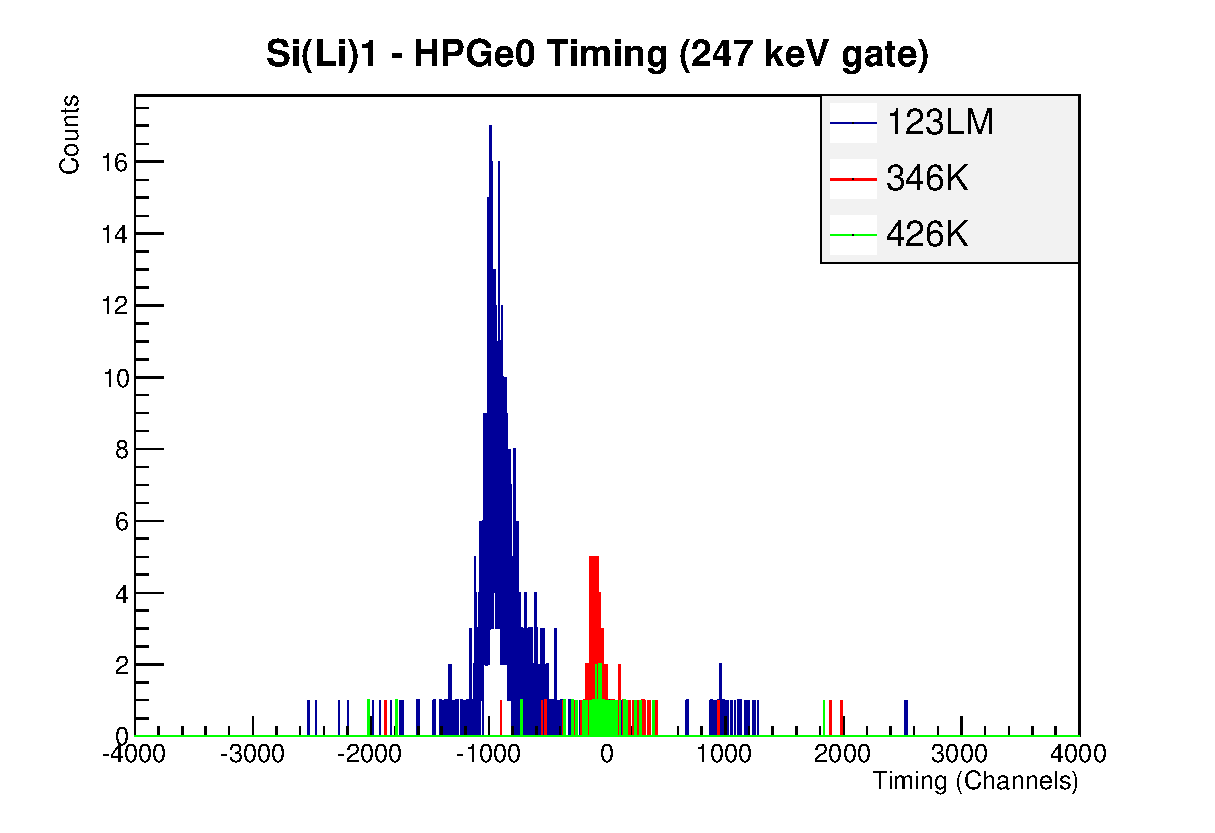
\includegraphics[scale=0.7]{Analysis_Figs/TimingvEnergy.eps}
    \caption[Timing example for the GEORGINA setup]{A plot of the energy-gated timing for a HPGe-Si(Li) detector pairing. The HPGe detector was gated at 247.9 keV, one of the ground state band transitions in the $^{145}$Gd nucleus. The conversion electrons for other transitions in the ground state band were gated on in the Si(Li) detector. Plotted here are the time differences between the two detectors when both peaks were seen in the respective detectors. The 123LM peak was used instead of the K peak due to the high threshold of this detector. As can be seen, the timing has an energy dependence. This dependence is most prominent at lower energies.}
    \label{fig:timing_georgina}
\end{figure}

In the Clovershare data, the timing was done within the electronics, leading to an clean structure, seen in Figure \ref{fig:timing_clover}. Although the same code structure was used for the timing, the gates were all the same within the Clovershare data. The main gate used was $\pm0.3$ and the background ranged from 0.3 to 0.9, using the same scaling as seen in Figure \ref{fig:timing_clover}.

\begin{figure}
    \centering
    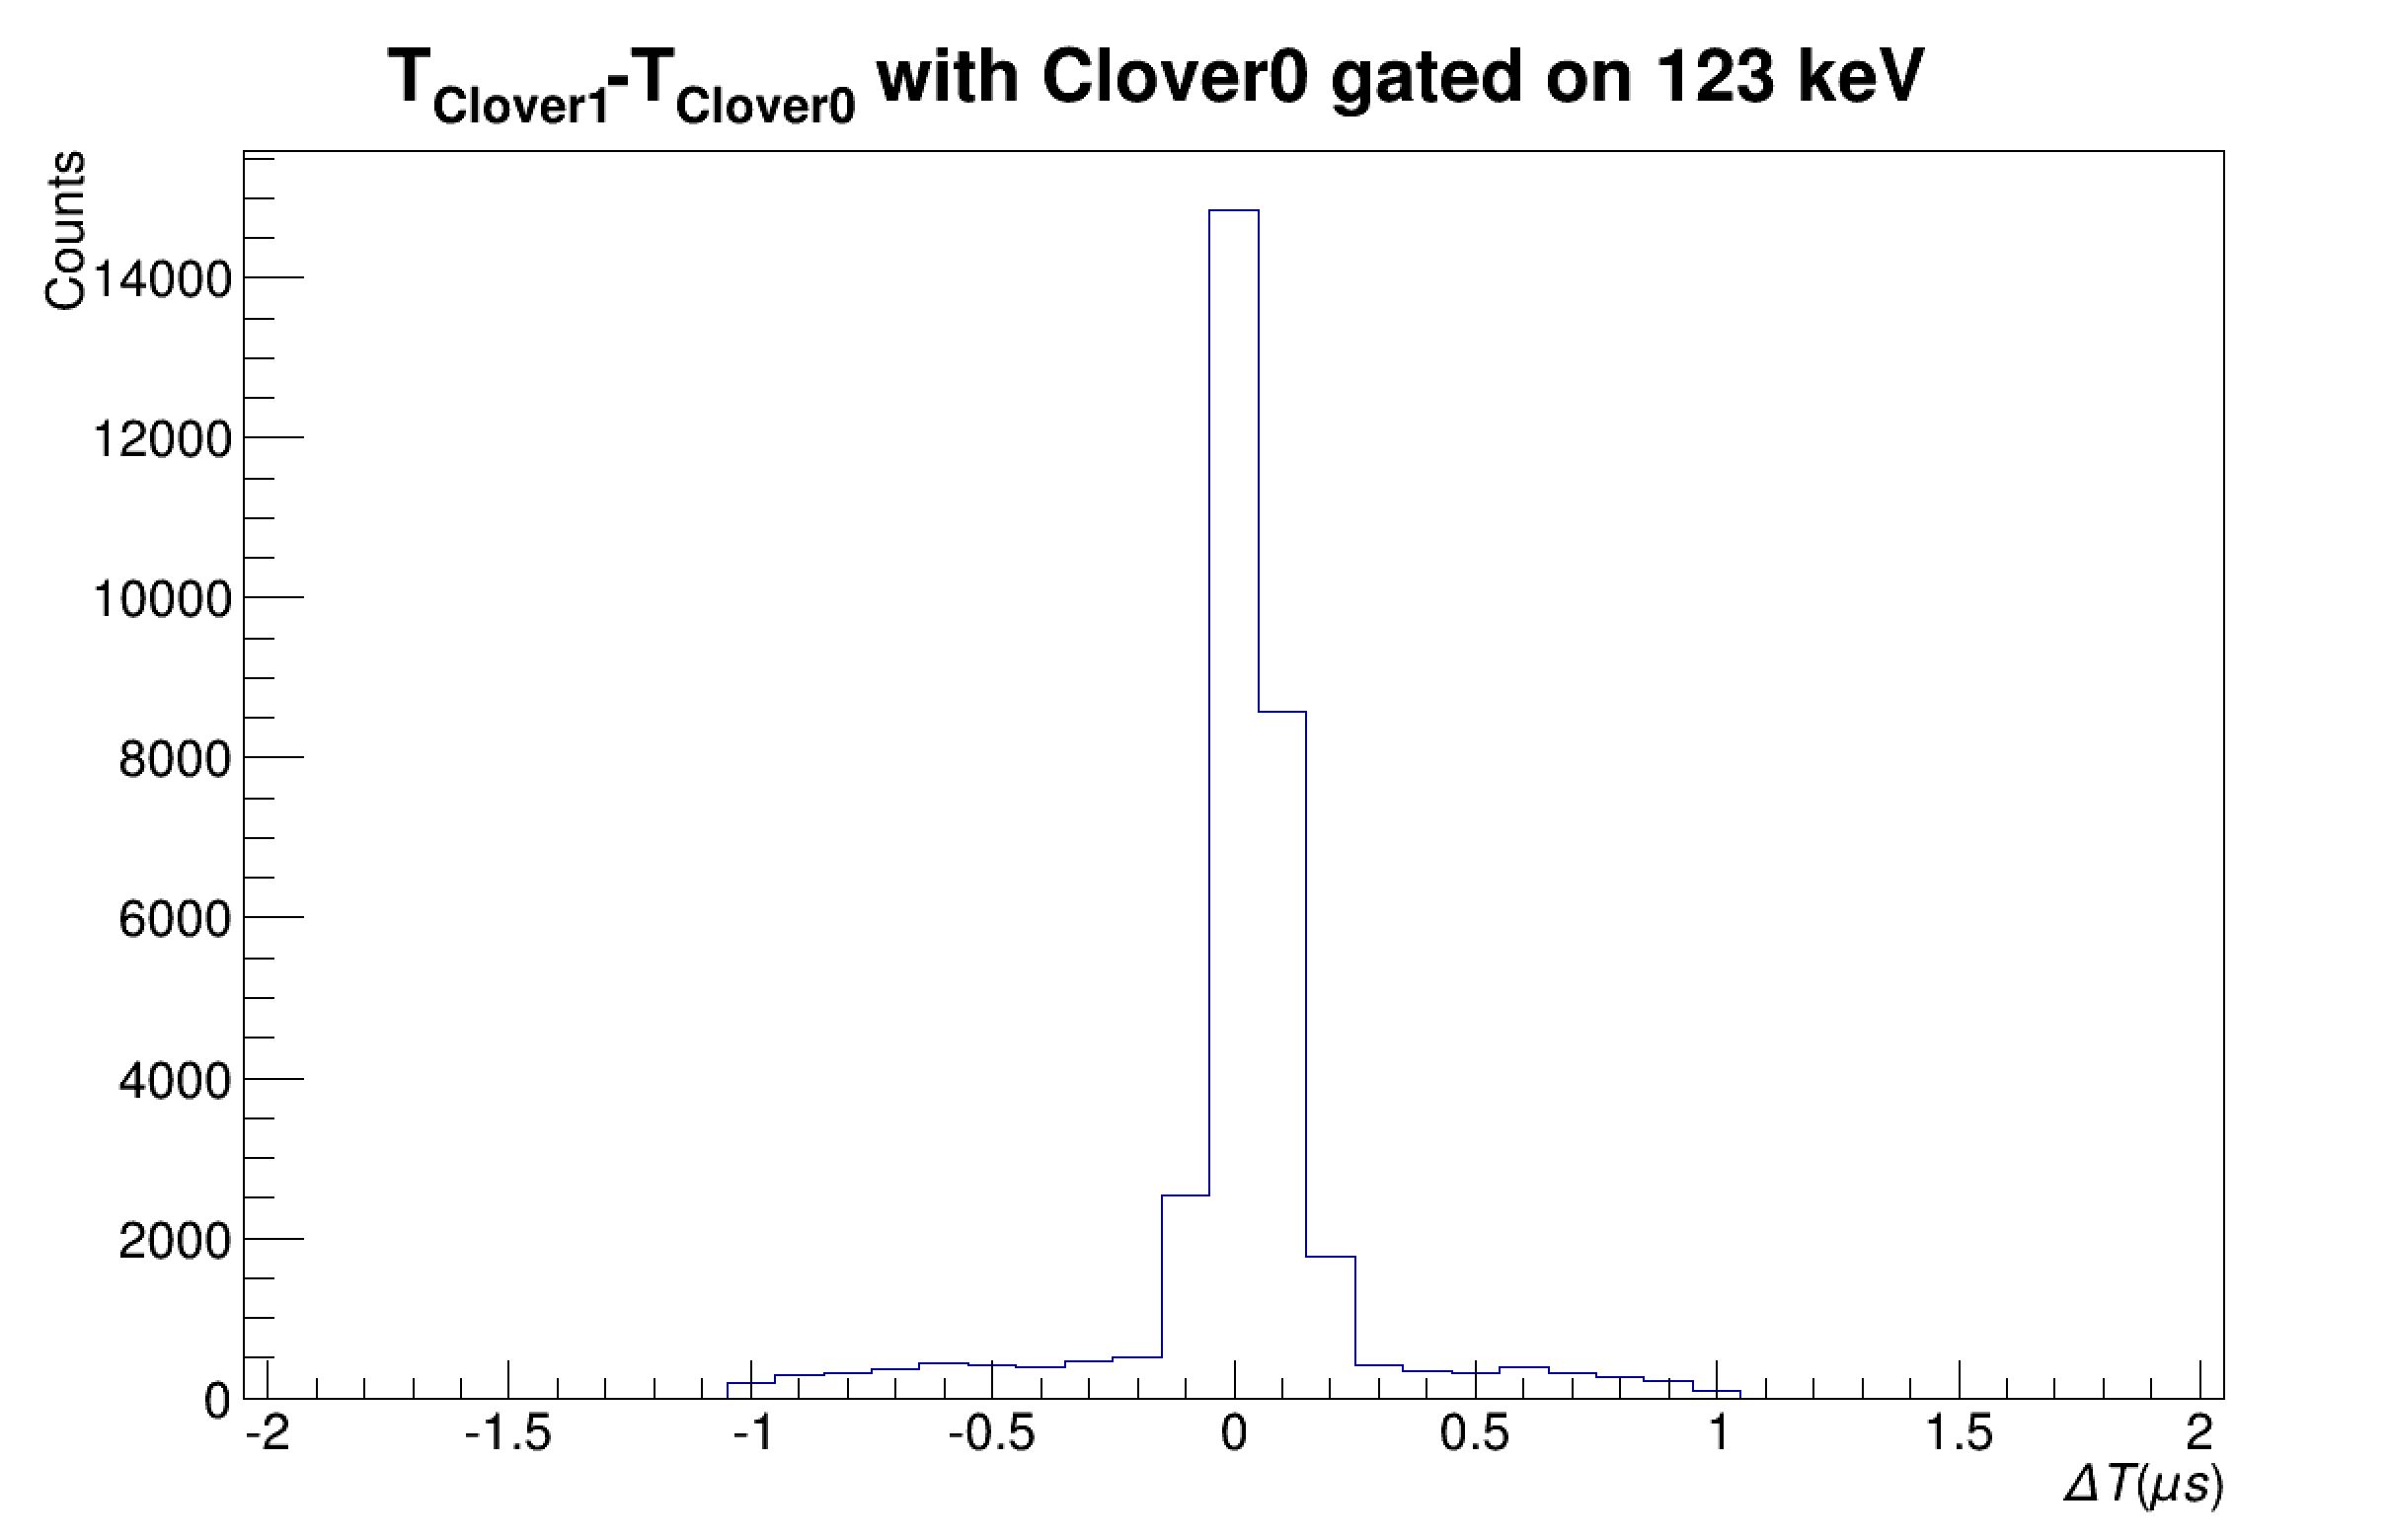
\includegraphics[scale=0.3]{Analysis_Figs/timing_clover.png}
    \caption{Timing between two of the Clovershare detectors, with one detector gated on 123 keV, the lowest transition in the ground state band of $^{154}$Gd. In this data, the gates all looked similarly symmetric, and the timing gates did not need to be varied as they had for the GEORGINA set up.}
    \label{fig:timing_clover}
\end{figure}

\section{Systematic Effects}

Several systematic effects had to be taken into account at various stages of analysis. Each will be discussed in further detail in this section. At the calibration stage, there are two major corrections in the Clovershare data. The first, as discussed in section \ref{sec:clover_cal}, is due to the integral non-linearities of the electronics. Second, the instability of the Clovershare detectors required a run-by-run calibration correction. 

In the analysis stage, corrections on extracted values needed to be done based on the angular correlations due to the detectors being at different angles relative to each other. If the angle between the two HPGe detectors were the same as the angle between the HPGe detector and Si(Li) detector(s), this correction would divide out and be unneeded.

\subsection{Electronics-based Integral Non-Linearities}

There are two kinds of non-linearities from electronics: integral and differential \citep{knoll00:rad_det_meas}. These two non-linearities are interrelated. Integral linearity is most easily seen in the energy calibration. Differential non-linearity can be seen by looking at the count rate with respect to channel number. [FIGURE FROM KNOLL?] Generally, the non-linearity can be expressed in calibration by a higher order correction to an otherwise linear calibration. In the GEORGINA detectors, this was the case. In the Clovershare detectors, this was not the case. 

The Pixie-16 MCA used in the Clovershare experiments has non-linearity specifications for 12-bit and 14-bit modes, but not 16-bit, according to the XIA datasheet \citep{xia:_pixie}. These are listed in terms of the difference of the least significant bit (LSB). In an ideal ADC, this number is 0, meaning the difference between two adjacent channels is exactly one LSB. A larger number means the gap is that much greater than one, and a negative number is that much less. When such non-linearities exist, a best case scenario is for the difference to be constant, leading to the polynomial correction. In the case of the Clovershare experiments, the LSB difference between channels does not appear to be constant.

Plotting the residuals of the calibration after doing a linear fit shows what appears to be a sawtooth pattern to the energy points, as seen in Figure \ref{fig:Clover_ene_res}. To fit this sawtooth pattern, it was assumed that the upward slope of the various sections was the same, and the sections were connected via the error function and complimentary error function, to allow for smoothing of the discontinuity. This results in the function

\begin{equation}
    \begin{aligned}
    	E_{res}= m*x+b_1*Erfc\left(\frac{x-f_1}{c}\right)+b_2*Erf\left(\frac{x-f_1}{c}\right)*\\Erfc\left(\frac{x-f_2}{c}\right)+b_3*Erfc\left(\frac{x-f_2}{c}\right)
    \end{aligned}
\end{equation}

where $m$ is the slope, $b_i$ are the various intercepts to shift the correction, $f_i$ is the location of the shift, and $c$ is the curvature of the error function.

\subsection{Run-based Calibration Corrections}

Run-by-run corrections are usually needed when there is drift or instability in the electronics or pre-amplifier. In the Si(Li) and GEORGINA detectors, there was no noticable drift. The Clovershare data does appear to need a correction for the HPGe detectors. The best way to track these instabilities was to look at known lines in each run, and plot the residuals after calibration, compared to the known value. This can be seen in Figure \ref{fig:clover_run}.  Several well defined peaks were taken in run to define a linear correction for each run. These linear corrections were done on top of the original energy calibration and correction.

\begin{figure}
    \centering
    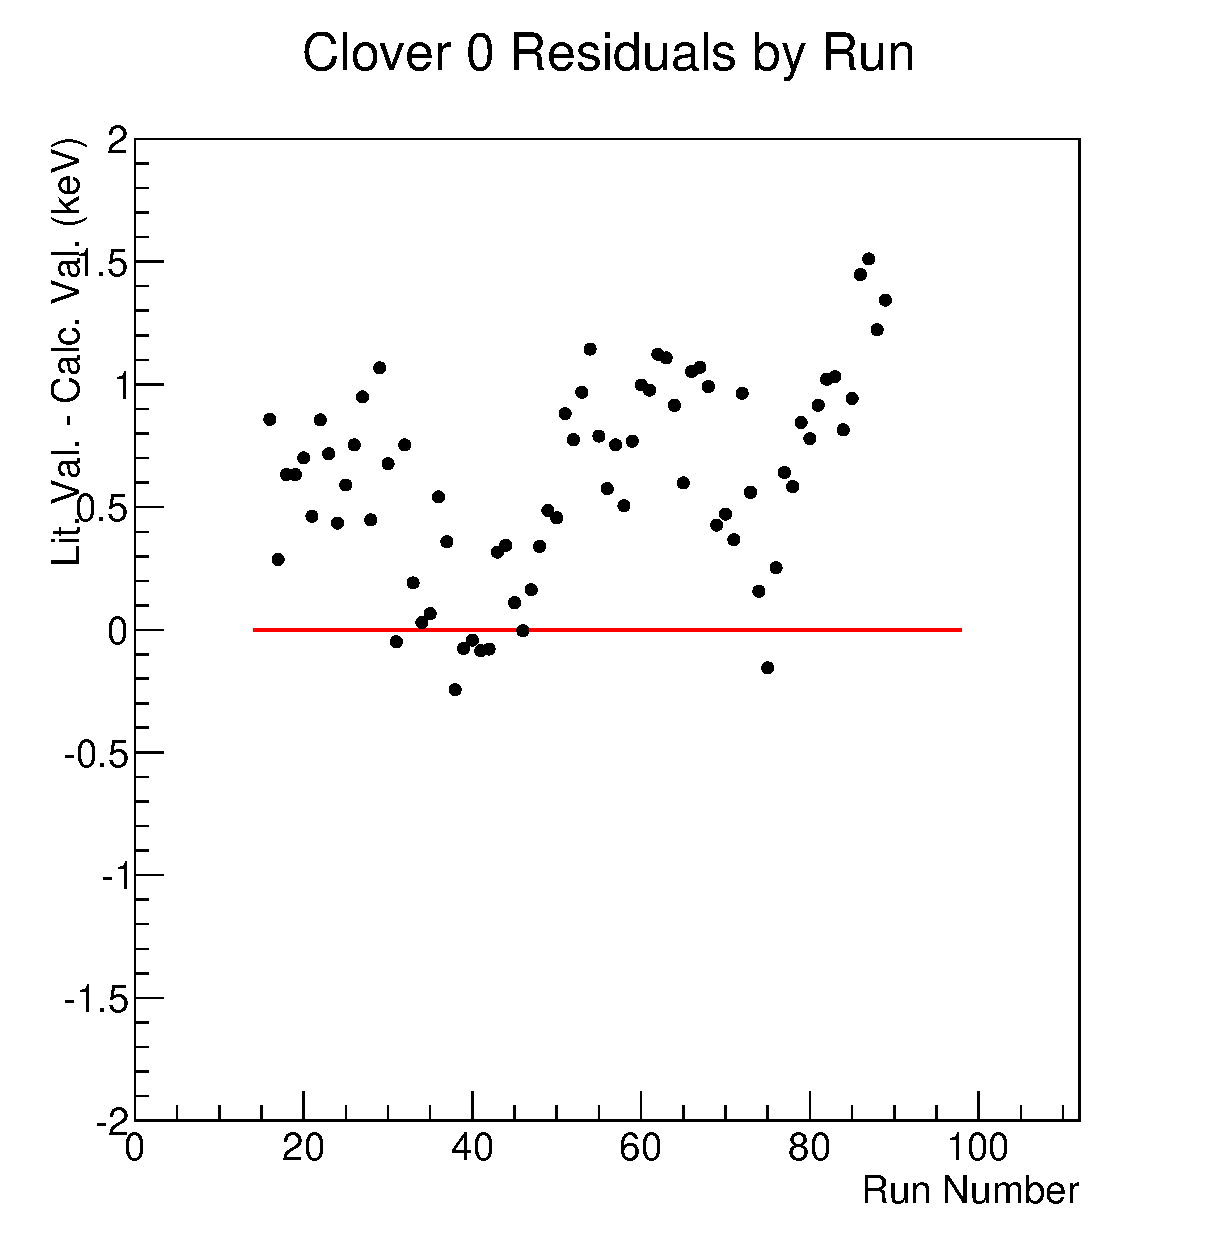
\includegraphics[scale=0.6]{Analysis_Figs/residual_by_run.eps}
    \caption[Example of calibration drift by run.]{The difference between the literature value and the calibrated value (before run-by-run correction) of the naturally occurring $^{40}$K background peak at 1460 keV, plotted by run for one leaf of one HPGe detector. The red line shows $\Delta E=0$.}
    \label{fig:clover_run}
\end{figure}

The peaks used for the run-by-run correction were a combination of the ground-state band peaks in the isotope of interest at low energies, and background gammas at higher energies, such as 1460 keV from $^{40}$K and 1764 keV from $^{214}$Bi. These are naturally occuring from the concrete walls of the NSL.

\subsection{Angular Correlations}

Angular correlations are a well studied phenomenon that arises when trying to look at two types of radiation in coincidence. A thorough exploration of different radiation pairings is explored in \citep{biedenharn53:_theory_angular_corr}. For this work, the pairings of interest are $\gamma-\gamma$ and $\gamma-e$. Triple correlations were also explored, as there were several cases where the intermediate transition was not seen.

Because the detectors are at different angles with respect to each other, when computing conversion coefficients, or subtracting off conversion electrons from the ground state band within the spectra, a correlation must be made based on these relative angles. Table \ref{tab:rel_angle_g} lists these angles from the ICEBall-Georgina setup, with respect to Detector 1. 

These angles can be calculated using

\begin{equation}
    \theta ' = cos^{-1}(\frac{sin\theta_1 cos\phi_1 sin\theta_2 cos\phi_2 +cos\theta_1 cos\phi_1 cos\theta_2 cos\phi_2 + sin\phi_1 sin\phi_2}{\sqrt{2}})
    \label{eq:rel_angle}
\end{equation}

with the previous definitions given for the angles in Tables \ref{tab:ICE_Det_Loc} and \ref{tab:GEORGE_Det_Loc}.

\begin{table}[]
    \centering
    \caption{Relative Angles of Detectors}
    \begin{tabular}{c|c} \toprule
         Detector & $\theta '$  \\
         \hline 
         HPGe 2 & 180 \\
         SiLi 1 & 90\\
         SiLi 2 & 90\\
         SiLi 3 & 122.5\\
         SiLi 4 & 110.7\\
         SiLi 5 & 69.3 \\
         SiLi 6 & 57.3 \\ \bottomrule
    \end{tabular}
    \footnotesize
    \item Relative angles of the detectors with respect to HPGe 1 in the ICEBall-GEORGINA set up. The angles were calculated using Tables \ref{tab:ICE_Det_Loc} and \ref{tab:GEORGE_Det_Loc} and equation \ref{eq:rel_angle_g}. All angles are in degrees.
    \label{tab:rel_angle_g}
\end{table}

Angular correlation functions for $\gamma-\gamma$ are usually written as a series of Legendre polynomials, multiplied by a correlation coefficient $A_\nu$, or

\begin{equation}
    w(\beta) = \sum_\nu A_\nu P_\nu(cos\beta)
    \label{eq:ge_corr}
\end{equation}

In the case of $\gamma-e$ correlations, the equation becomes 

\begin{equation}
    \begin{split}
        w_m(\beta) = \sum_\nu b_\nu(LLm) A_\nu P_\nu(cos\beta), \\
        w_e(\beta) = \sum_\nu b_\nu(L+1,L+1,e) A_\nu P_\nu(cos\beta)
        \label{eq:e_corr}
    \end{split}
\end{equation}

depending on if the radiation is electric or magnetic in nature. The $b_\nu$ values are based off the same matrix elements used to calculate theoretical conversion coefficients, and are well understood\citep{rose51:_internal_conversion, rose52:_internal_conversion}.

Both of these cases assume pure multipole transitions. In the case of mixed transitions, the correlation function becomes

\begin{equation}
    W = w_I + \delta^2 w_{II} + 2\delta w_{III}
    \label{eq:mixed_corr}
\end{equation}

where $w_I$ and $w_{II}$ are the pure multipole correlation functions, and $w_{III}$ is a correlation mixing the two multipoles. The variable $\delta$ is known as the mixing ratio. 

These correlations can be further extrapolated to look at cases not just of direct correlations, but of indirect correlations, such as three $\gamma$-rays in cascade. If the middle radiation is not observed, the first and third radiations still have a determinable correlation. This is derived for pure multipoles by \citep{biedenharn53:_theory_angular_corr} and for mixed transitions by \citep{rose53:_angular_corr_supp,osborn53:_angular_corr_3}.

\section{Upper Limits}
\label{sec:upper_limit}

In $^{156}$Gd, there were several possible transitions of interest at energies less than 250 keV. In that energy range, the ground-state band transitions cover much of the spectrum. Some transitions could be removed through the use of gating on gamma-rays of parallel transitions, but not all the transitions could be removed. This was due, in part, to the gate transitions being in sequence with some of the ground-state band. 

To get an upper limit for the transitions of interest, the ground state band transitions that were in sequence with the gate transition were subtracted off of the conversion electron spectrum through the following method. An example of this subtraction can be seen in Figure \ref{fig:subtraction} The skewed gaussian fitting function described earlier was given parameters derived from the data and subtracted from the conversion electron spectrum.

\begin{figure}
    \centering
    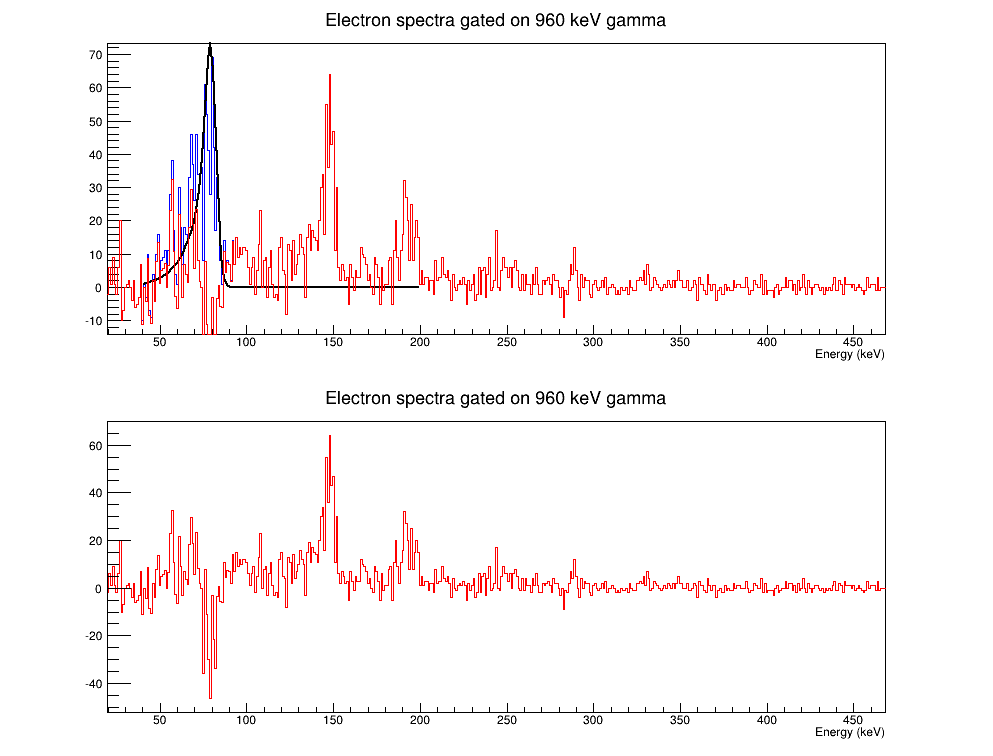
\includegraphics[scale=0.4]{Analysis_Figs/Subtraction_SiLiAll_960.png}
    \caption{An example of the subtraction used to removed the ground state band peaks from spectra. To subtract the conversion electron peak off, the area of the corresponding gamma peak was taken from the same gate. Using the conversion coefficient and the efficiencies of both detectors, the area of the peak could be calculated. From there, this value, along with fixed $R$, $\beta$, $\sigma$, and centroid were used to subtract the peak off. The black line is the function used for subtraction. The blue line is the original spectrum, and the red liine is after subtraction. This code can be found in Appendix \ref{chap:macros}.}
    \label{fig:subtraction}
\end{figure}

The area of the skewed gaussian is obtained by getting the area of the gamma peak, and adjusting by several factors: efficiencies ($\epsilon$), conversion coefficient ($\alpha$, as derived from theory), and correlation coefficients ($W$). This gives the following:

\begin{equation}
    A_{ce} = A_{\gamma}\times\frac{\epsilon_{ce}}{\epsilon_{\gamma}}\times\alpha\times\frac{W_{ce}}{W_{\gamma}}
    \label{eq:subt_area_skew}
\end{equation}

The height of the skewed gaussian can be derived in terms of the area, $R$, $\sigma$ and $\beta$ to be

\begin{equation}
    H = A\frac{100}{2*e^{-\frac{\sigma^2}{2\beta^2}}R\sigma-\sqrt{2\pi}(R-100)\sigma};
    \label{eq:subt_height_skew}
\end{equation}

These three variables are all unique to the detector, and come directly from fitting the calibration data, as previously discussed. From there, the parameters can be fed into the equation, along with the centroid of the peak, and subtracted directly off the spectrum. Any remaining counts are counted by taking sections on either side of the area of interest and using a global linear fit for the background, as seen in Figure \ref{fig:piecewise}. This linear fit is subtracted off bin-by-bin in the region of interest. The remaining area is then taken as an upper limit on the transition of interest.

\begin{figure}
    \centering
    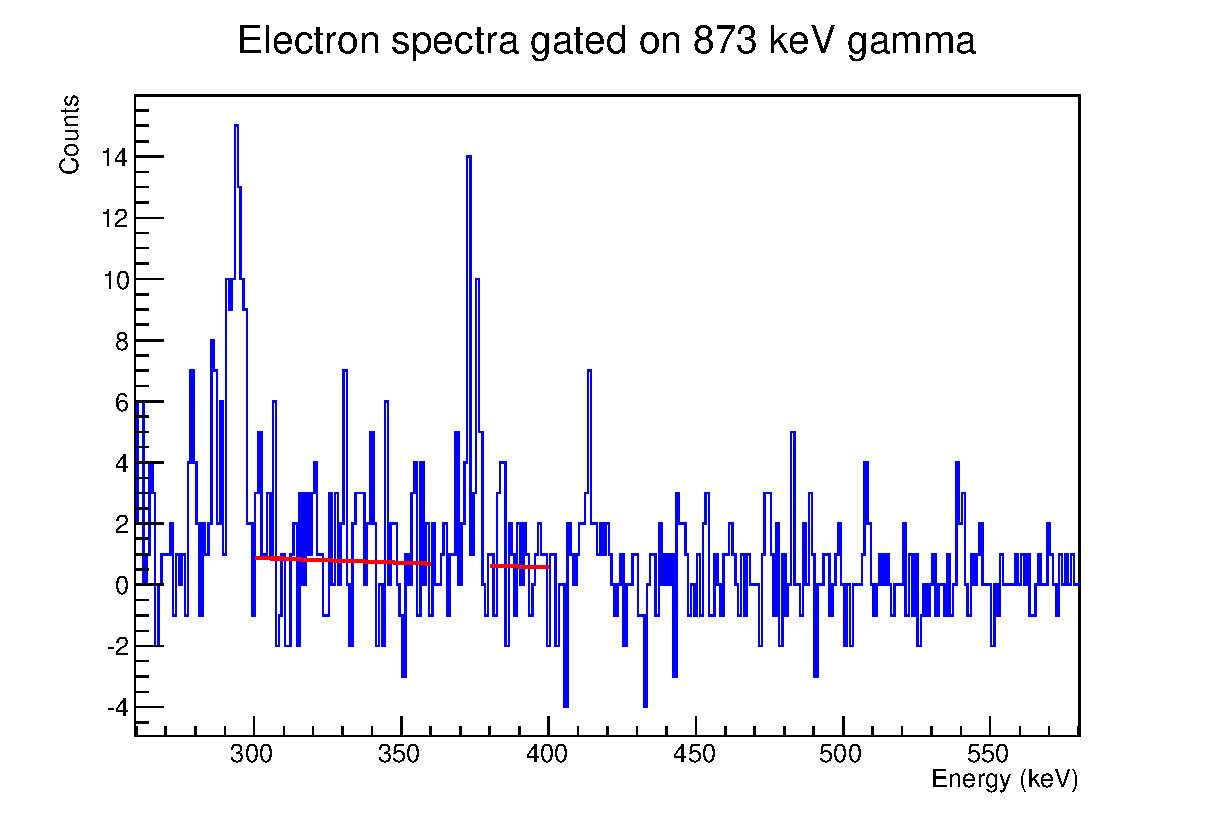
\includegraphics[scale=0.6]{Analysis_Figs/Piecewise_example.eps}
    \caption{An example of the global background fit used for peaks that could not be fit using the skewed gaussian function. The areas on either side of the peak are selected by the user. Once the background fit is done, the central area between the two sections is treated as the peak and the background is subtracted off to give a peak area. The red line shows the fit for the background area, and the two sections used for the background fit. See \ref{chap:macros} for the global-fit function used.}
    \label{fig:piecewise}
\end{figure}

\section{Error Analysis}

When areas of peaks were found, the error is found with the fit. In the cases of the peaks that needed to be fit by estimating the background and subtracting it off, the error of the area is assumed to be the square root of the level.

These areas are propagated through calculations via the equation

\begin{equation}
    \sigma_{f}^2=\sum_{i}\left(\sigma_{x_i}\frac{\delta f}{\delta_{x_i}}\right)^2
\end{equation}

where $f$ is a function of all $x_i$ in the sum \citep{bevington03:_error}. If the function is related to all variables via some form of a polynomial, i.e. $(x_i)^a$ where $a$ is a constant, then it can be rewritten as

\begin{equation}
    \sigma_{f}^2=f*\sum_{i}\left(\frac{\sigma_{x_i}}{a*x_i}\right)^2
\end{equation}

Errors on the areas of both gamma-rays and electrons were propagated through the data. The error on the efficiency was estimated by shifting the efficiency value $\pm0.5\sigma$ and calculating upper and lower limit functions for the efficiency. 

In the final results, the uncertainties were kept separate into statistical and systematic effects. Statistical effects are caused by the areas of the peaks. Systematic effects are from the uncertainty in the efficiency of both the HPGe and Si(Li) detectors, as well as an uncertainty in the angular correlations, based on the solid angle covered by the detectors.

%
% Chapter 4
%

\chapter{$^{154}$Gd Results}
\label{chap:154Gd}

$^{154}$Gd is a transitional nucleus ($\beta_2=0.3105$) with a large number of $0^+$ states identified by $(p,t)$, 16, under 3 MeV\citep{meyer06:_zeroplus}. Eleven of these $0^+$ states are below the pairing gap (the energy required to remove two like nucleons), as shown in Figure \ref{fig:Gd_Sys}. The nature of these $0^+$ states is of interest for this study. The lowest lying excited $0^+$ state in the nucleus has an anomalously large E2 transition to the ground state, as compared with other nuclei in the region, shown in Figure \ref{fig:Gd_Sys}. For this $0^+$ state, there is a question of the state being a $\beta$-vibration built upon the ground state, or the minimum of another shape configuration.

\afterpage{\clearpage\begin{landscape}
\begin{figurels}
    \centering
    \caption{Systematics of the Gadolinium isotopes. $^{154}$Gd has an anomalously large connection between the first excited $0^+$ state and the ground state. The arrows shown are the B(E2) components of the transitions, in single particle Weisskopf units \citep{reich09:_nds_154,reich12:_nds_156,nica17:_nds_158,reich05:_nds_160}. The $R_{4/2}$ values beneath each nucleus are a ratio of the energies of the first excited $2^+$ and $4^+$ states, both in the ground state band. This ratio gives a rough measure of deformation.}
    \label{fig:Gd_Sys}
\end{figurels}
% \addtocounter{figure}{-1}
\begin{figurels}
    \centering
    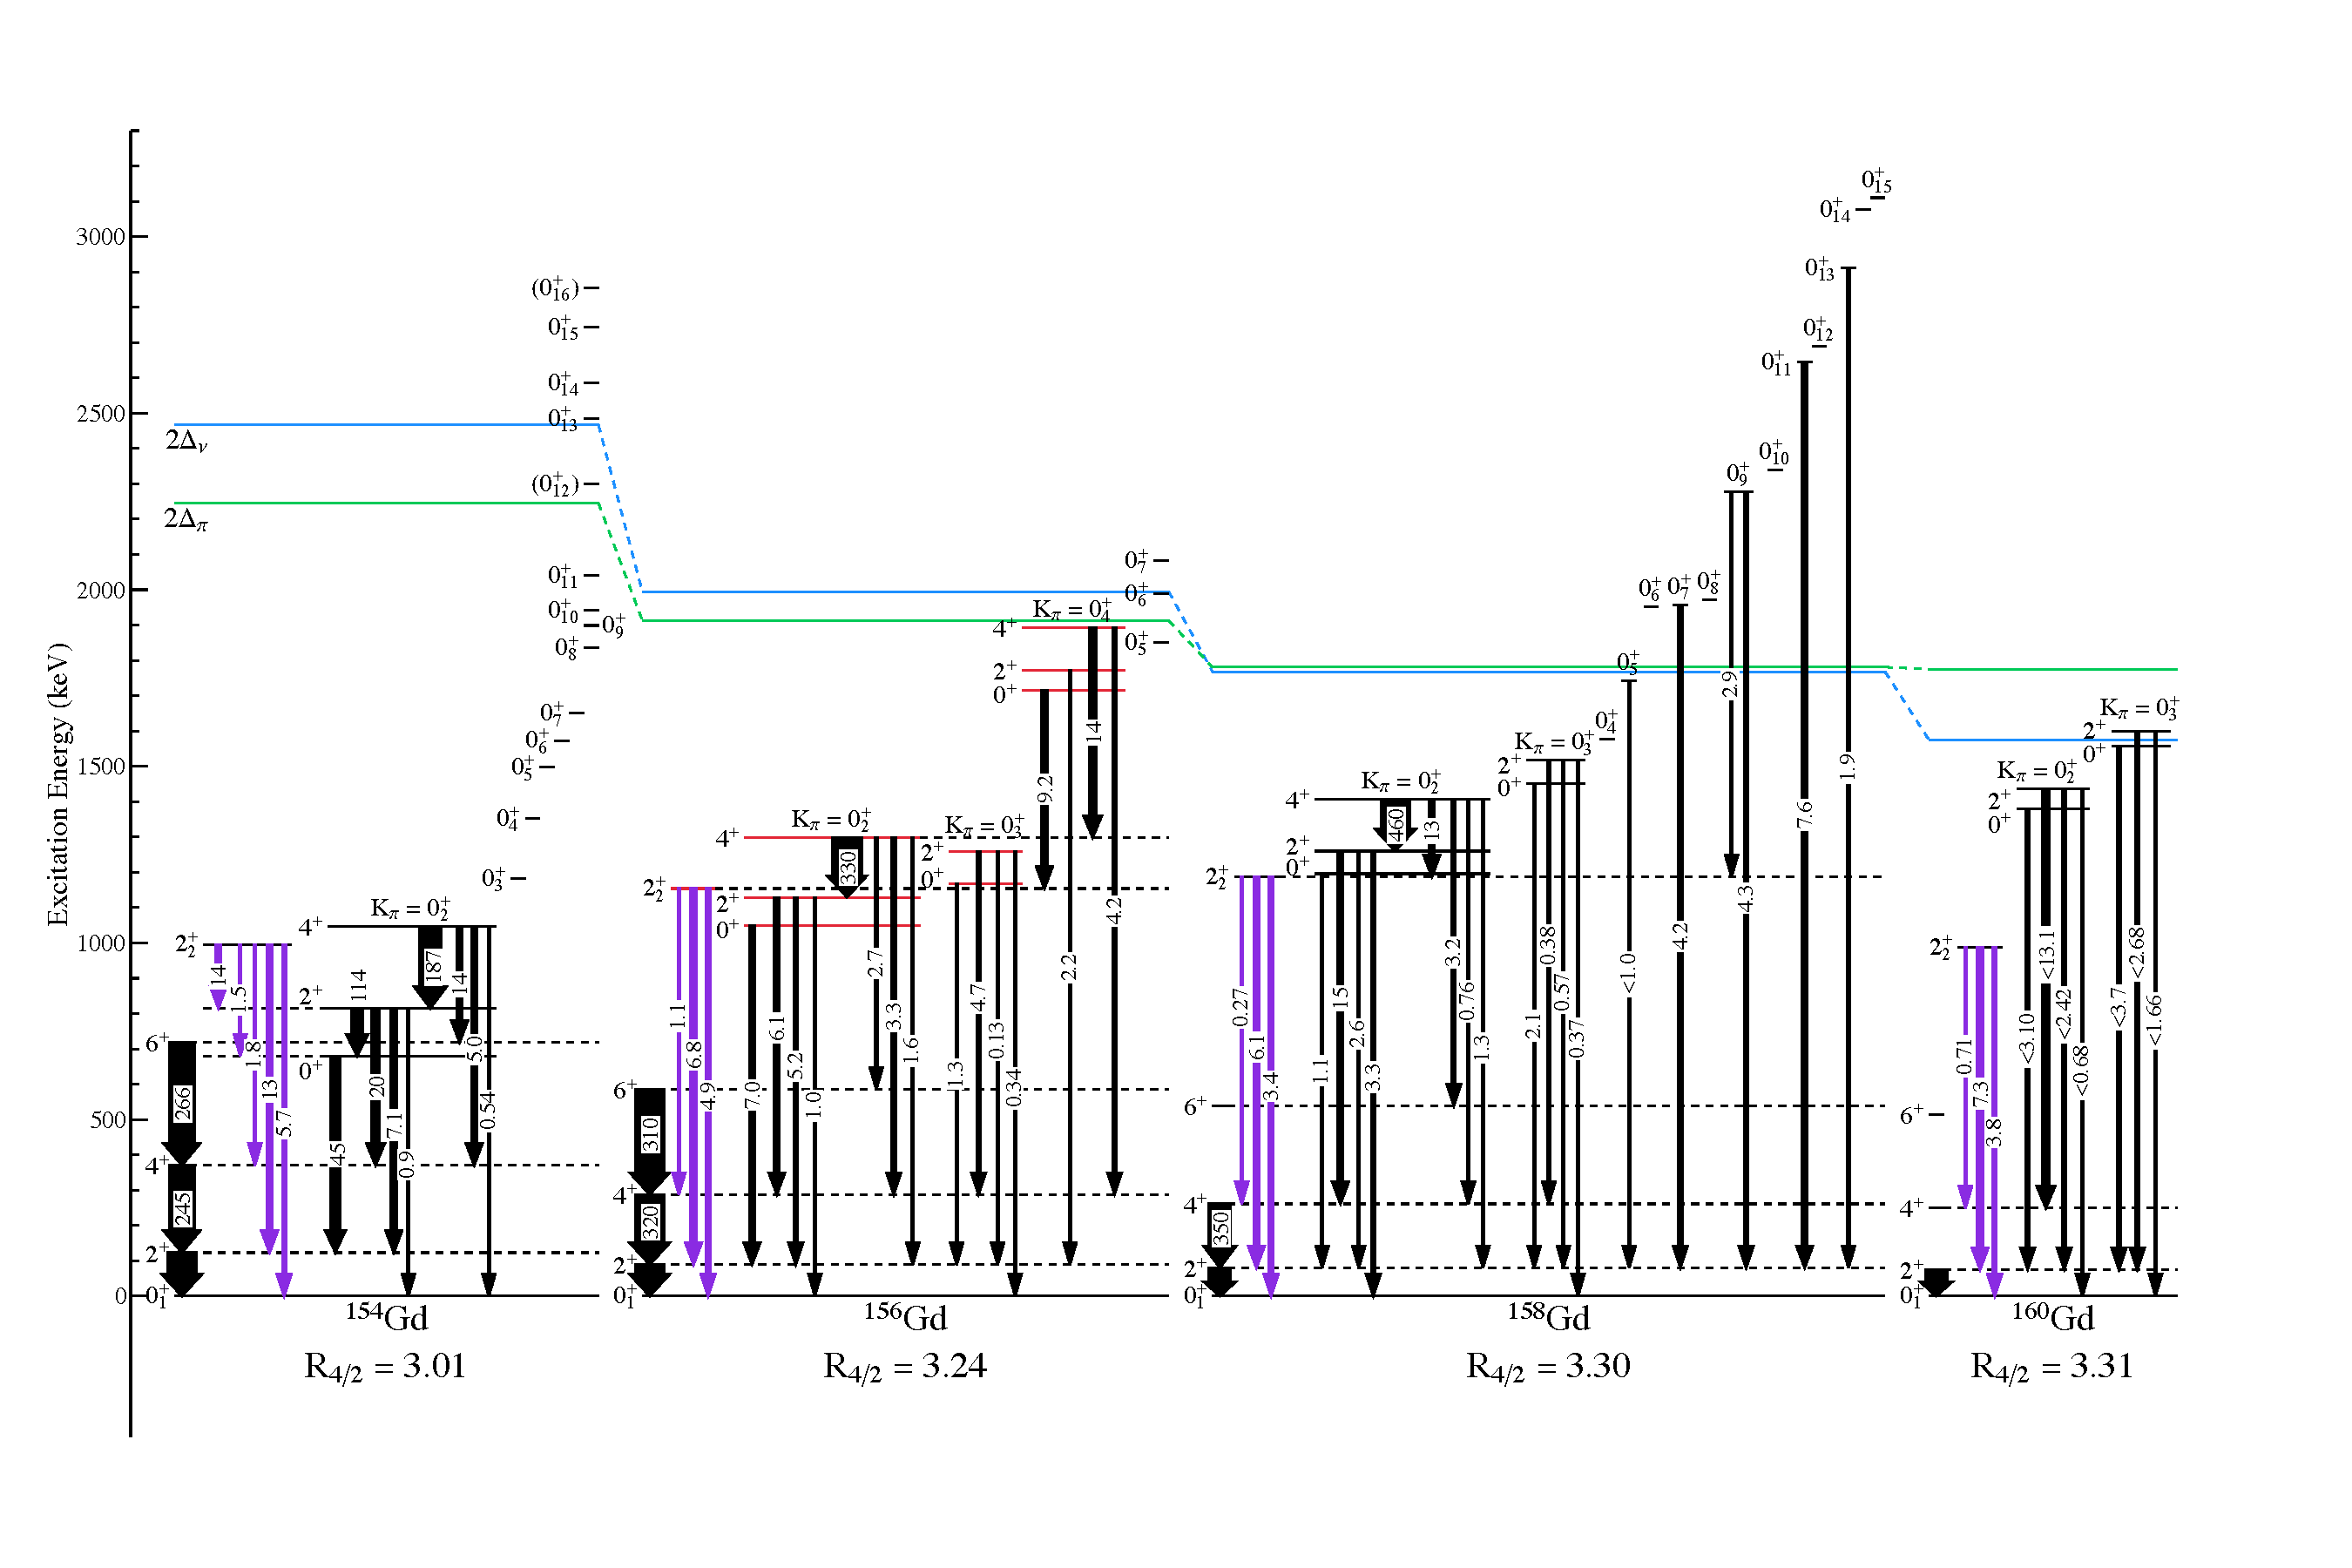
\includegraphics[width=1.35\textwidth]{154GdTablesAndFigs/Gd_Schematic_v2.pdf}
\end{figurels}
\end{landscape}}

The $^{154}$Gd data was taken across three separate runs; one with ICEBall and GEORGINA, and two with ICEBall and Clovershare, in two different configurations, as discussed in Chapter \ref{chap:setup}. The GEORGINA experiment allowed for the HPGe detectors to be closer to the target, at a distance of 30 cm. This experiment yielded the most conversion electron data, and results in this chapter are quoted from that data. Although the Clovershare detectors had to be placed 5-10 cm farther from the target, the larger number of detectors, 7 for the first run and 5 for the second, resulted in better the $\gamma-\gamma$ coincidence data, so identification of transition placements and level populations are confirmed. All of the experiments used the same enriched $^{152}$Sm target of 1.44 $mg/cm^2$ thickness, discussed in Chapter \ref{chap:setup} and shown in Table \ref{tab:target}. A complete catalog of spectra used in the analysis can be found in Appendix \ref{chap:154_spectra}.

\section{Ground State Band Confirmation}
\label{sec:154GS_Confirm}

In the singles spectrum several prominent peaks stand out, as seen in Figure \ref{fig:154Gd_Singles}. In the $\gamma$-spectrum, there are four prominent peaks from 100 to 500 keV. These peaks are the ground state band. The strong peak just beyond 500 keV is the 511 keV annihilation peak, and the peaks below 100 keV are x-rays. In the conversion electron spectrum of Figure \ref{fig:154Gd_Singles}, there are distinguishable peaks until approximately 400 keV, and then again in the range of 550 keV to 650 keV. The peaks up to 400 keV correspond to these same ground-state lines that are prominent in the $\gamma$-spectrum. The $K$ peaks are 51 keV less than the $\gamma$-peak, due to electron binding energy. The $L$ peaks are 8 keV less, while the $M$ peaks and higher electron shells are 1 keV or less different, compared to the energy of the $\gamma$-peak. The peaks in the range of 550 keV to 650 keV correspond to a strong series of $J^{\pi}\rightarrow J^{\pi}$ transitions from the first excited $0^+$ band.

\afterpage{\clearpage\begin{figure}[!]
    \centering
    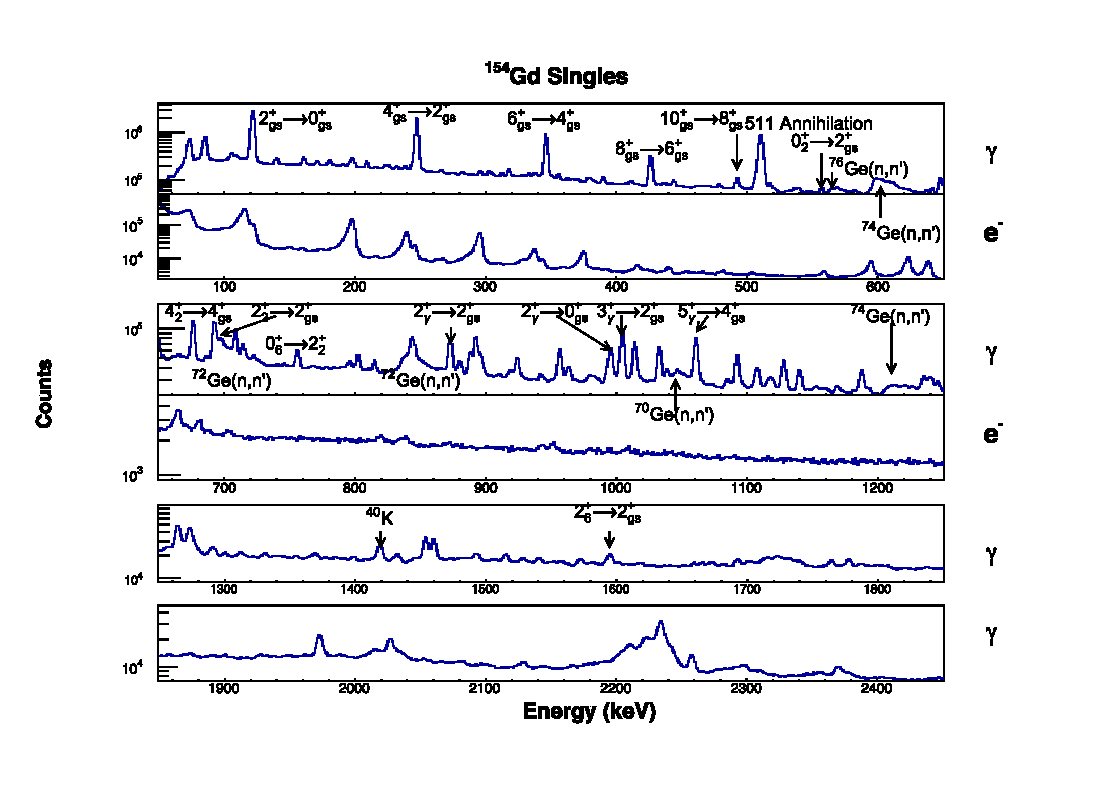
\includegraphics[scale=0.9]{154GdTablesAndFigs/154Gd_Singles_Label.eps}
    \caption[Singles spectra of $^{154}$Gd]{Singles spectra of $^{154}$Gd. Spectra are labeled with the particles being detected, the energies of the $\gamma$ and electron spectra aligned for identification. In the $\gamma$ spectrum, several lines of note are labeled. These are the ground-state band lines. In the conversion electron spectrum, the large peaks up to approximately 450 keV are from the ground state band. These large peaks make the ground state band a good diagnostic, but also emphasize the need for coincidence gating, as the conversion electron spectrum is flooded by the ground state band electrons. The large peak at low energy is cut off due to the threshold. It is a combination of background and the 123K peak. Transitions in the higher energy regime of the $\gamma$ spectrum cannot be determined without gating, due to additional background from the experimental room.}
    \label{fig:154Gd_Singles}
\end{figure}}

These ground state band transitions are known to be pure E2 multipoles, and have been previously measured and identified as such. This makes them excellent for calibration and comparison with calculated theoretical conversion coefficients.

In gated spectra, the internal conversion coefficients for the ground state band were in agreement with theory, after the angular correlation correction, discussed in Section \ref{sec:angular}, was applied. The peaks corresponding to the ground state band did not have contributions from other transitions when gated. In the singles, two of the four ground state band lines overestimated the conversion coefficient, indicating electron contributions from other transitions.  To remove the contributions from other transitions, the $\gamma$-ray had to be distinguishable and identifable. The conversion coefficient was then assumed from theory, and the contribution to the area was calculated to be
\begin{equation}
    \label{eq:ICC_Subtract}
    A_{e} = \alpha \epsilon_{e} \frac{A_{\gamma}}{\epsilon_{\gamma}} C_{\angle}
\end{equation}
where $\epsilon_{i}$ are the efficiencies of the electrons and gammas respectively. $C_{\angle}$ is the angular correction for this particular transition, discussed in Section \ref{sec:angular}.

For the $6_{gs}^+\rightarrow 4_{gs}^+$ and $8_{gs}^+\rightarrow 6_{gs}^+$ transitions, electron contributions from smaller gamma lines of similar energy had to be subtracted. Looking at Figure \ref{fig:154Gd_Singles}, it is clear there are many transitions around the same energy, making determination of the contributing peaks important. Only lines from reactions in the target material will contribute. Potential contribution lines needed to be identified as coming from the reaction. This is done by gating on the lines and identifying them within the known level scheme,  as is discussed in Section \ref{sec:154GS_Gates}. For instance, the 390.73 keV line in Table \ref{tab:154Gd_Contaminants}, was seen in coincidence with the $4^+_{gs}\rightarrow2^+_{gs}$, $6^+_{gs}\rightarrow4^+_{gs}$, $4^+_{0^+_{2}}\rightarrow2^+_{gs}$, $6^+_{0^+_{2}}\rightarrow6^+_{gs}$, $4^+_{0^+_{2}}\rightarrow4^+_{gs}$, $6^+_{0^+_{2}}\rightarrow4^+_{0^+_{2}}$, and $10^+_{0^+_{2}}\rightarrow8^+_{0^+_{2}}$ transitions. The transitions involving the ground state band gave context for approximate $J^{\pi}$, as no ground state band lines were seen above the $6^+$ state.  The transitions between the $0^+_{2}$ band and the ground state band indicates the 390.73 keV line is part of the $0^+_{2}$ band. Finally, seeing both the $6^+_{0^+_{2}}\rightarrow4^+_{0^+_{2}}$, and $10^+_{0^+_{2}}\rightarrow8^+_{0^+_{2}}$ transitions without the intermediate transition, which matched in energy, gave firm identification. Multipolarities could then be assigned based on the known data, and the contribution to the electron peak of interest could be calculated based on the gamma area and theoretical conversion coefficient. Contributions were subtracted off the fitted area of the electron peak, before the conversion coefficient of the ground state line was calculated. The error also includes contributions from the errors of these extra transitions' gamma peaks and the errors on the theoretical $\alpha$ values. 

There were two types of transitions that contributed to the conversion electron peak areas: those of similar energy, and higher energies whose K-electron energies were similar to the L and M peaks of the lines of interest. The peaks are summarized in Table \ref{tab:154Gd_Contaminants}. The electron-shell of the transition is listed in each case, and total $L$ and $M$ contributions are used, without need to look at subshell contributions.  In several transitions, the mixing ratio had to be assumed to get a conversion coefficient for the subtraction.

\afterpage{\clearpage\begin{table}[!]
    \centering
    \begin{longtable}{>{\small}c|>{\small}c|>{\small}c|>{\small}c|>{\small}c|>{\small}c|>{\small}c|>{\small}c}
        \caption{$^{154}$Gd Ground State Band $6^+\rightarrow 4^+$ and $8^+\rightarrow 6^+$ Extra Electron Peak Contributions in Singles}
        \label{tab:154Gd_Contaminants} \\
        \toprule
         $E$ & $E_i$ & $E_f$ & $J_i\rightarrow J_f$ & Multipolarity & $\delta$ & Shell & $\alpha$  \\ \hline
         \endhead
         \endfoot
         \endlastfoot
         \multicolumn{8}{l}{346.59 keV, $6^+\rightarrow 4^+$} \\ \hline
         338.28 & 1770 & 1432 & $5^+_{4^+}\rightarrow 5^+_{\gamma}$ & E0,E2,M1 & -0.004 & K & 0.10 (1) \\ 
         & & & & & $\frac{K(E0)}{K(E2)}\approx 1.0$ & L & 0.01210 (12) \\ 
         & & & & & & M & 0.00180 (3) \\ \hline
         342.18 & 2254 & 1911 & $8^+_{4^+}\rightarrow 6^+_{4^+}$ & E2 & & K & 0.0315 (5) \\ 
         & & & & & & L & 0.0069 (1) \\\
         & & & & & & M & 0.001554 (22) \\ \hline
         390.73 & 1756 & 1366 & $8^+_{0^+_2}\rightarrow 6^+_{0^+_2}$ & E2 & & K & 0.0218 (3) \\ \hline
         \multicolumn{8}{l}{426.84 keV, $8^+\rightarrow 6^+$} \\ \hline
         422.12 & 1418 & 996 & $2^+_{0^+_3}\rightarrow 2^+_{\gamma}$ & E0,E2,M1 & Assumed $\approx 1$ & K & 0.114 (16) \\ 
         & & & & & & L & 0.0161 (23) \\ 
         & & & & & & M & 0.0049 (12) \\ \hline
         466.99 & 1719 & 1251 & $2^-_{2^-}\rightarrow 3^-_{0^-}$ & M1,E2 & Assumed $\approx 1$ & K & 0.019 (6) \\ \hline
         478.27 & 1719 & 1241 & $2^-_{2^-}\rightarrow 1^-_{0^-}$ & E2 & & K & 0.01272 (18) \\
         \bottomrule
         \multicolumn{8}{p{\textwidth}}{Table \ref{tab:154Gd_Contaminants}: A list of the transitions in the $^{154}$Gd Singles data that were contributing to the electron peaks corresponding to the ground state band lines. Conversion coefficients were assumed using BrICC\citep{kibedi08:_BRICC}. The bands for each level are listed as subscripts.}
    \end{longtable}
\end{table}}

The $6_{gs}^+\rightarrow 4_{gs}^+$ K-conversion coefficient was 0.0546(1)(14) before contributions from other transitions were taken into account. After subtracting the transitions in Table \ref{tab:154Gd_Contaminants}, the new value is 0.0335(1)$^{+11}_{-10}$, in agreement with previous measurements and theory from BrICC\citep{kibedi08:_BRICC}. Similarly, the $8_{gs}^+\rightarrow 6_{gs}^+$ K-conversion coefficient went 0.0271(2)(7) to 0.0180(2)(5), also in agreement with theory calculations. The contributing transitions that were subtracted are summarized in Table \ref{tab:154Gd_Contaminants}.  The conversion coefficient was then calculated, with an angular distribution correction based on the multipolarity of the transition. The transitions up to the $10_{gs}^+$ are summarized and compared with theory in Table \ref{tab:154Gd_Single_ICC_GS}.

\afterpage{\clearpage\begin{landscape}
    \begin{longtable}{c|c|c|c|c|c|c|c|c|c|c}
        \caption{$^{154}$Gd Ground State Band Internal Conversion Coefficients from Singles}
        \label{tab:154Gd_Single_ICC_GS}\\
        \toprule
        $E$ (keV)	&	$J^{\pi}	\rightarrow	J^{\pi}$	&	$E_i$ (keV)	&	$E_f$ (keV)	&	$T_{1/2}$ (fs)	&	Multipolarity & Shell &	$\alpha$ (This Work)				&	$\alpha$  (Th)	&	$\alpha$ (Spits) & $\alpha$ (Gono)		\\
        \hline
        \endfirsthead
        \caption[]{$^{154}$Gd Ground State Band Internal Conversion Coefficients from Singles}\\
        \toprule
        $E$ (keV)	&	$J^{\pi}	\rightarrow	J^{\pi}$	&	$E_i$ (keV)	&	$E_f$ (keV)	&	$T_{1/2}$ (fs)	&	Multipolarity	& Shell &	$\alpha$ (This Work)				&	$\alpha$  (Th)	&	$\alpha$ (Spits) & $\alpha$ (Gono)	\\
        \hline
	    \endhead
	    \hline
        122.23	&	$2^+	\rightarrow	0^+$	&	123.0709	&	0	&	1184000	&	E2	&	K &	0.7759 (34) $^{+148}_{-146}$	&	0.656 (10)	& 0.61 (3) &		\\
    	&				&		&			&		&	& L	&	0.3788 (26) $^{+81}_{-80}$	&	0.411 (6)	&	&	\\
	    &				&		&		&			&	& M	&	0.1323 (3) (29)	&	0.0963 (14)	&	&	\\
	    \hline
        247.85	&	$4^+	\rightarrow	2^+$	&	370.9998	&	123.0709	&	45600	&	E2	&	K &	0.1044	(2) $^{+31}_{-30}$	&	0.1000 (12)	&	0.080 (3)	& 0.0827 (119)\\
	    &				&		&		&		& &	L	&	0.0272	(1) (8)	&	0.0225 (4)	&		\\
	    &				&		&		&		& & M	&	0.0096	(1) (3)	&	0.00513 (8)	&		\\
	    \hline
        346.59$^\dagger$	&	$6^+	\rightarrow	4^+$	&	717.662	&	370.9998	&	8260	&	E2 & K &	0.0335	(1)$^{+11}_{-10}$	&	0.0304 (5)	&	0.029 (1) & 0.0306*	\\
	    &				&		&		&		&	& L	&	0.0087	(1) (3)	&	0.00662 (10)	&		\\
	    &				&		&		&		&	& M	&	0.0027	(1)	(1) &	0.001491 (21)	&		\\
	    \hline
        426.84$^\dagger$	&	$8^+	\rightarrow	6^+$	&	1144.44	&	717.662	&	2570	&	[E2] & K & 0.0180	(2) (5)	&	0.01716 (24)	&	& 0.0170 (22)	\\
    	&				&		&		&		&	& L	&	0.0030	(1) (1)	&	0.00332 (5)	&		\\
	    &				&		&		&		&  	& M	&	0.0008	(1)	(1) &	0.000741 (11)	&		\\
	    \hline
        493.171	&	$10^+	\rightarrow	8^+$	&	1637.05	&	1144.44	&	1110	&	E2	& K	&	0.0124	(4) (4)	&	0.01179 (17)	& &	0.0124 (21)	\\
	    &				&		&		&		&	& L	&	0.0067	(4) (2)	&	0.00213 (3)	&		\\
        \bottomrule
    \end{longtable}
    \item{A list of ground state band conversion coefficients from $^{154}$Gd. Multipolarities and mixing ratios were taken from NNDC. Unless otherwise stated, the $\alpha$ values are $\alpha_K$. An angular distribution correction has been applied based on multipolarities for pure transitions, and those with known mixing ratios. The first error is statistical, the second is systematic. Numbers are compared with Spits et al.\citep{spits96:_154gd} and Gono et al.\citep{gono74:_154gd_e0} The starred value was used as an absolute calibration of the conversion electron detector in the Gono work. The dagger lines had contaminant lines subtracted from the conversion electrons. See the text for more details.}
\end{landscape}}

\section{Gates on the Ground State Band}
\label{sec:154GS_Gates}

To confirm the levels populated in the experiment, the $\gamma$-rays of the ground state transitions were used as energy gates. Figures \ref{fig:154_2to0}, \ref{fig:154_4to2}, \ref{fig:154_6to4}, and \ref{fig:154_8to6} are the level scheme result of these gates, with Figures \ref{fig:154_2to0spec}, \ref{fig:154_4to2spec}, \ref{fig:154_6to4spec}, and \ref{fig:154_8to6spec} being the corresponding gated spectra. Band structure in these figures was taken from the data sheets\citep{reich09:_nds_154}. No band assignments were made in this work. In the cases of cascades, secondary gates were done to confirm assignments. The spectra from these gates are available in Appendix \ref{chap:154_spectra}.

Determining which transitions went uniquely into a given ground state level was done by comparing the outgoing ground state transition for that level with the incoming transition i.e. for the $2^+$ level, the $2_{gs}^+\rightarrow 0_{gs}^+$ (123 keV) gate was compared directly with the $4_{gs}^+\rightarrow 2_{gs}^+$ (247 keV) gate. The $\gamma$-spectra corresponding to two of these gates can be seen in Figure \ref{fig:154_GS_Gate}. Lines in the gamma spectrum that were present only in the outgoing spectrum, but not the incoming, were assumed to be populating that level. For example, in Figure \ref{fig:154_GS_Gate}, several areas have been highlighted. The line at 557 keV is present in the $2_{gs}^+\rightarrow 0_{gs}^+$ gate, but not the $4_{gs}^+\rightarrow 2_{gs}^+$ gate. This line corresponds to the $0^+_{2}\rightarrow 2^+_{gs}$ transition, putting it in parallel with the $4_{gs}^+\rightarrow 2_{gs}^+$ transition, explaining why it remains unseen. These identified transitions were then gated on to confirm the assignment, and to search for cascades from higher states.

\afterpage{\clearpage\begin{landscape}
\begin{figurels}[!]
    \caption{\fontsize{10pt}{12pt} Spectra gated on 123 keV ($2_{gs}^+\rightarrow 0_{gs}^+$) and 247 keV ($4_{gs}^+\rightarrow 2_{gs}^+$), the first two ground state band lines of $^{154}$Gd. As can be seen, some lines do not appear in different gates. Comparison of these gates, yields a list of transitions that directly populate the interim level (in this example, the $2^+$ state). Several peaks are circled in green that appear in the $2_{gs}^+\rightarrow 0_{gs}^+$ and not the $4_{gs}^+\rightarrow 2_{gs}^+$ transition.}
    \label{fig:154_GS_Gate}
\end{figurels}
\begin{figurels}[!]
    \centering
    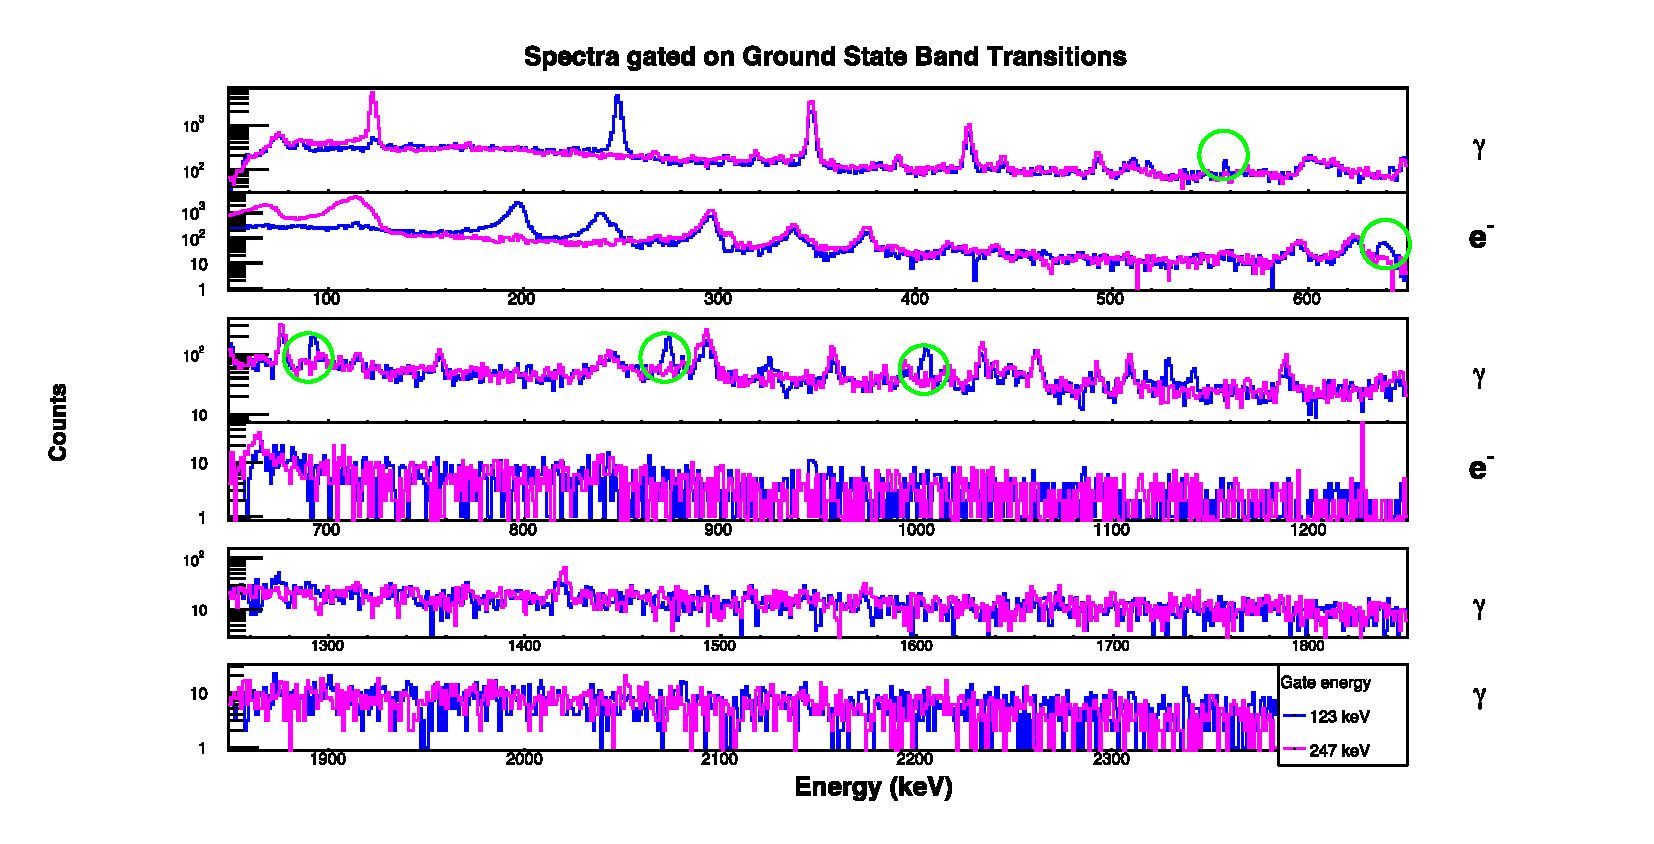
\includegraphics[scale=0.9]{154GdTablesAndFigs/154Gd_stacked.eps}
\end{figurels}
\end{landscape}}

There were nine bands seen in the gating, 4 of which are bands with excited $0^+$ band heads. These are seen in the $2^+_{gs}\rightarrow 0^+_{gs}$ gate (Figures \ref{fig:154_2to0} and \ref{fig:154_2to0spec}). Three of these bands are seen in the $4^+_{gs}\rightarrow 2^+_{gs}$ gate (Figures \ref{fig:154_4to2} and \ref{fig:154_4to2spec}), and two are seen in the $6^+_{gs}\rightarrow 4^+_{gs}$ gate (Figure Figures \ref{fig:154_6to4} and \ref{fig:154_6to4spec}). Only one is seen in the $8^+_{gs}\rightarrow 6^+_{gs}$ gate (Figures \ref{fig:154_8to6} and \ref{fig:154_8to6spec}). This drop off is unsurprising for multiple reasons. Studies have shown the $(\alpha,2n)$ reaction to stop populating spin states with a significant cross section beyond $J^{\pi}=12^+$ \citep{wu93:_a2n}. In the ground state band of $^{154}$Gd, the $12^+$ state sits at 2184.69 keV, giving an approximate cut off for populating higher energy states in the nucleus. Additionally, due to the lack of known higher spin states in the higher energy $0^+$ bands, identification of populating such bands in the higher gates becomes difficult.

\afterpage{\clearpage\begin{landscape}
\begin{figure}[!]
    \centering
    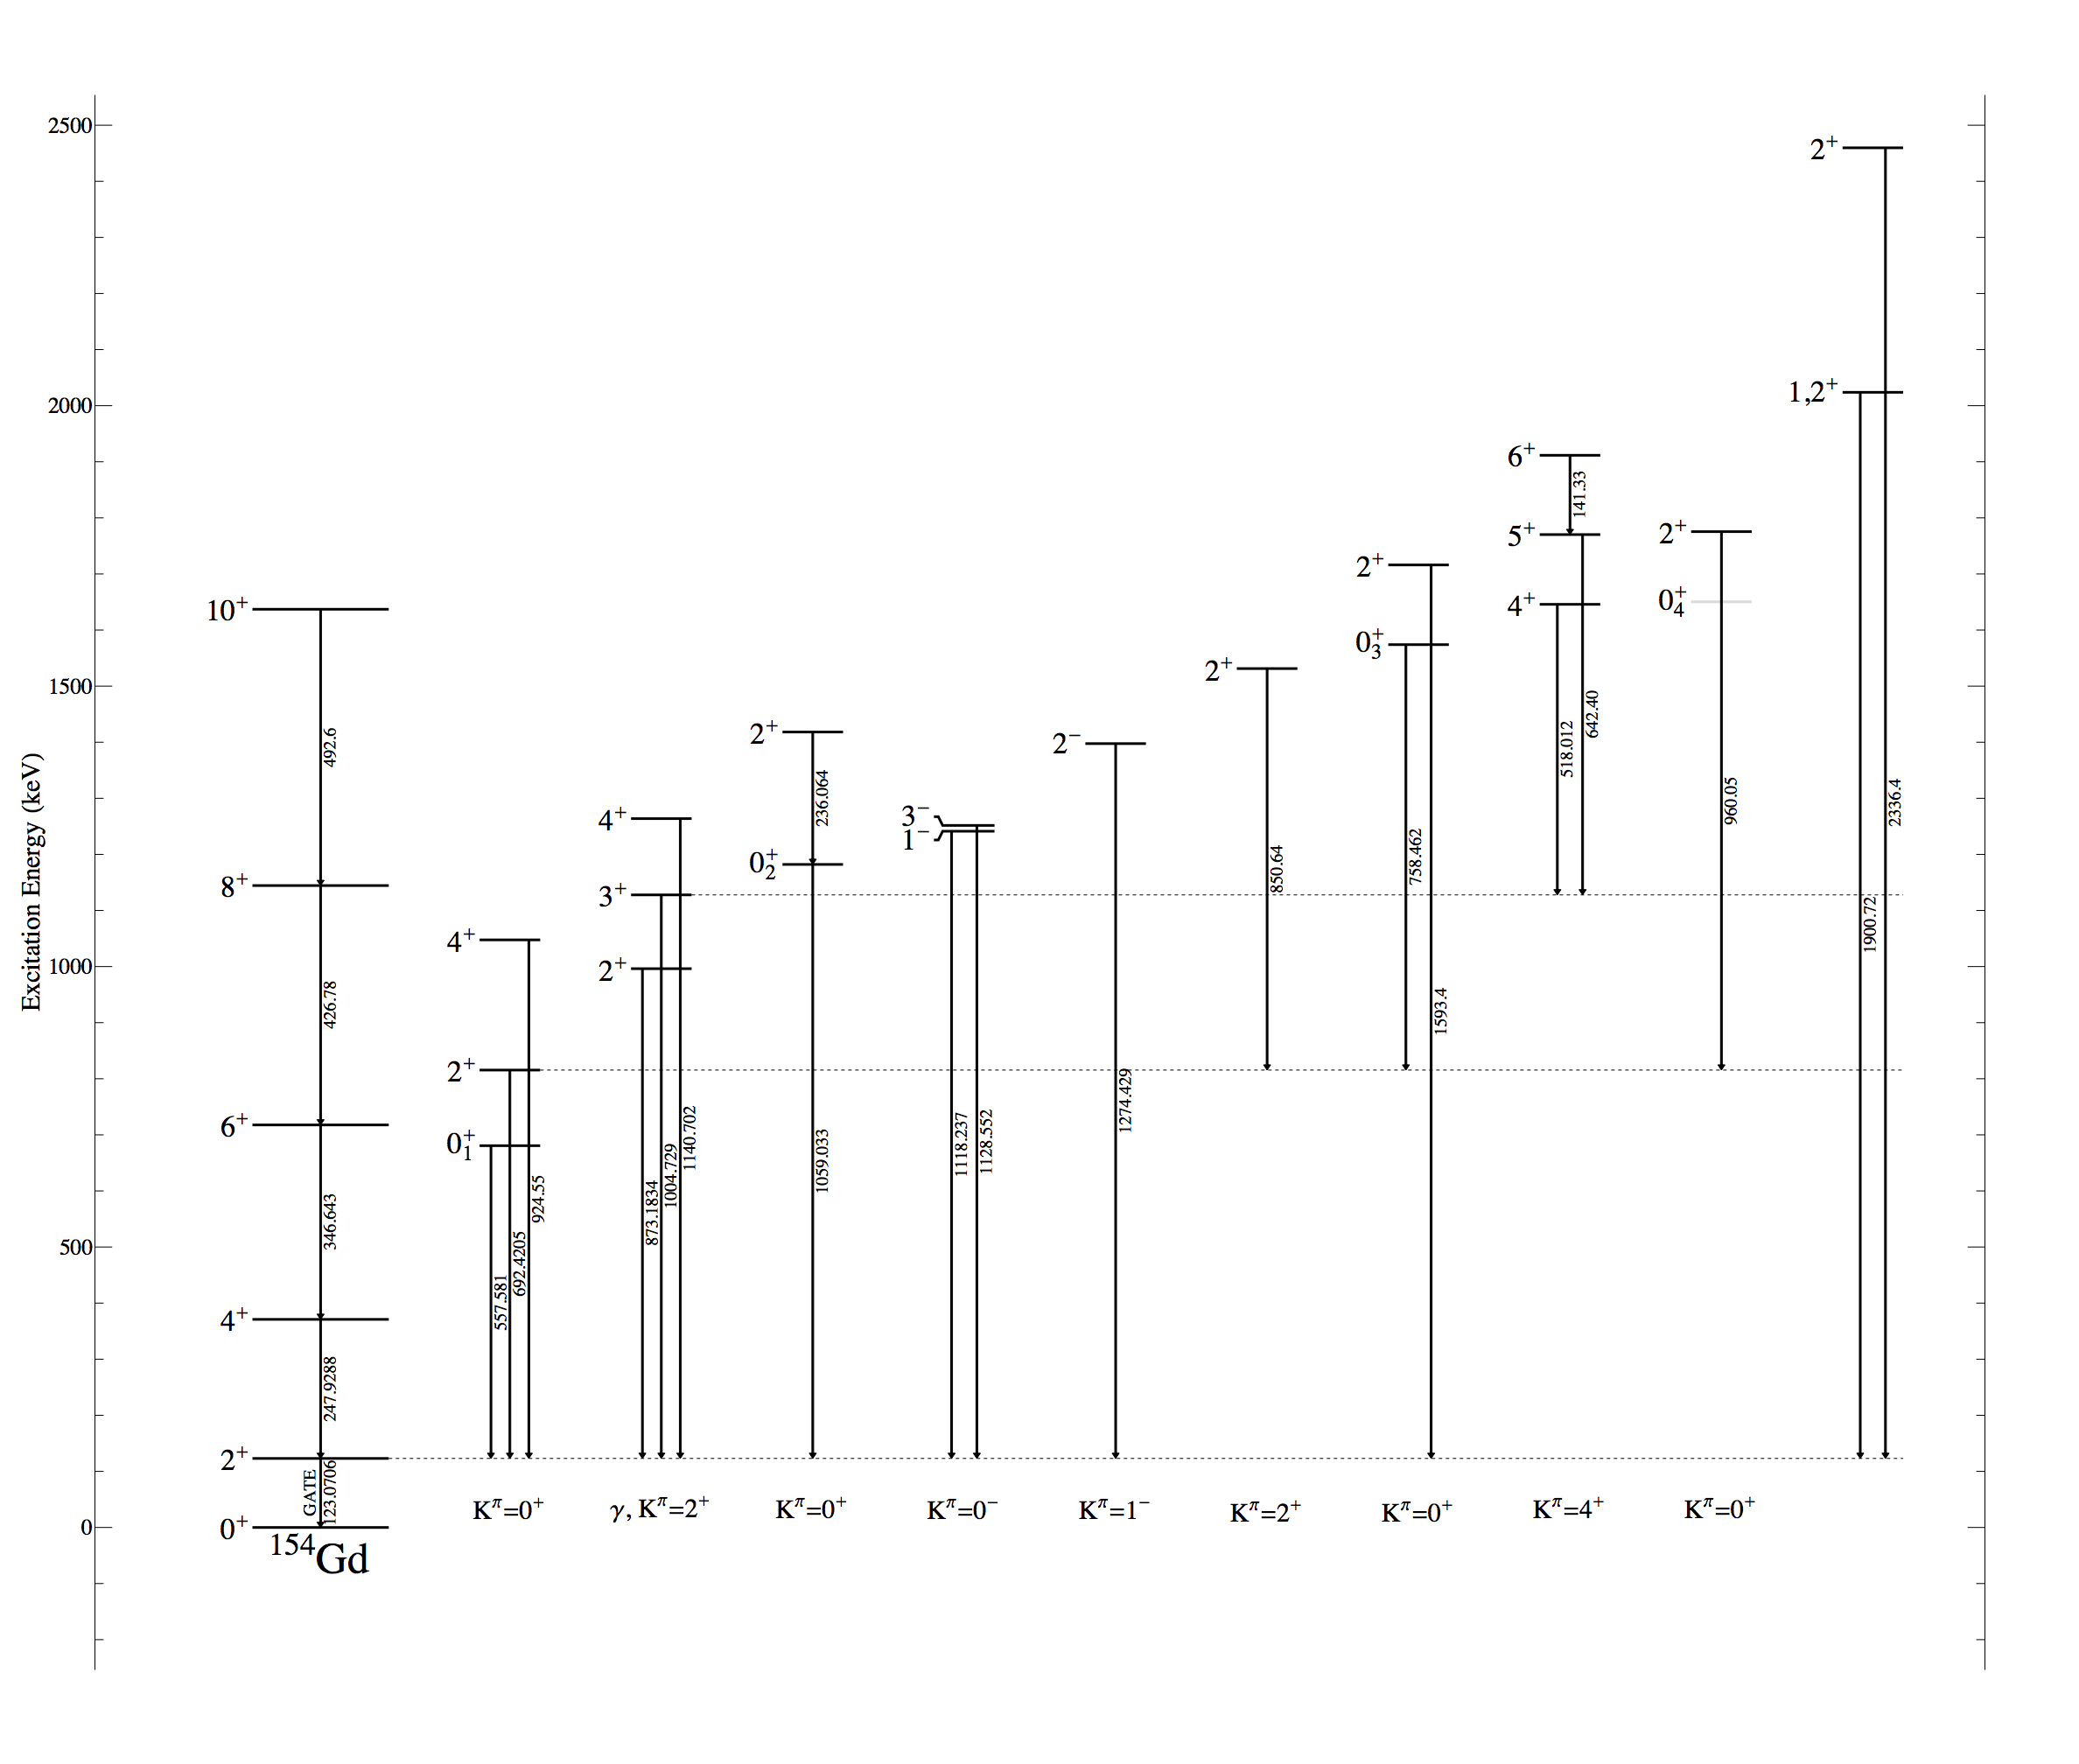
\includegraphics[scale=0.33]{154GdTablesAndFigs/154Gd_2to0.eps}
    \caption{Level Scheme of $^{154}$Gd. The gamma ray of the $2^+\rightarrow0^+$ transition (123 keV) in the ground state was gated on. It was then compared with the gated spectrum from the gamma ray of the $4^+\rightarrow2^+$ transition (247 keV) in the ground state. Peaks only appearing in the first gate and not higher energy gates were assumed to go into the $2^+$ state, and assignments were made. Due to the low energy of the $2^+\rightarrow0^+$ transition, the efficiency was lower, and it is likely that transitions into the $2^+$ state were missed. The levels are organized by band. The lower levels of the band, unseen by gamma rays in this gate, are in gray.}
    \label{fig:154_2to0}
\end{figure}
\end{landscape}}

\afterpage{\clearpage\begin{landscape}
\begin{figure}[!]
    \centering
    \captionlistentry{(a) Level Scheme of $^{154}$Gd. The gate on the $4_{gs}^+\rightarrow 2_{gs}^+$ transition (247 keV) $\gamma$-component in the ground state. The lines shown are in coincidence. The levels are organized by band. The lower levels of the band, unseen by gamma rays in this gate, are in blue. (b) Gamma spectrum gated on 247 keV, corresponding to the $4_{gs}^+\rightarrow 2_{gs}^+$ transition. Several transitions have been labeled, corresponding to the level scheme.}
    \label{fig:154_4to2}
    \begin{subfigure}{1.4\textwidth}
    \caption{\centering \fontsize{10pt}{12pt}Level Scheme of $^{154}$Gd. The gate on the $4_{gs}^+\rightarrow 2_{gs}^+$ transition (247 keV) $\gamma$-component in the ground state. The lines shown are in coincidence. The levels are organized by band. The lower levels of the band, unseen by gamma rays in this gate, are in blue. (b) Gamma spectrum gated on 247 keV, corresponding to the $4_{gs}^+\rightarrow 2_{gs}^+$ transition. Several transitions have been labeled, corresponding to the level scheme.}
    \end{subfigure}
\end{figure}
\clearpage
\begin{figure}
    \ContinuedFloat
    \begin{subfigure}{1.4\textwidth}
    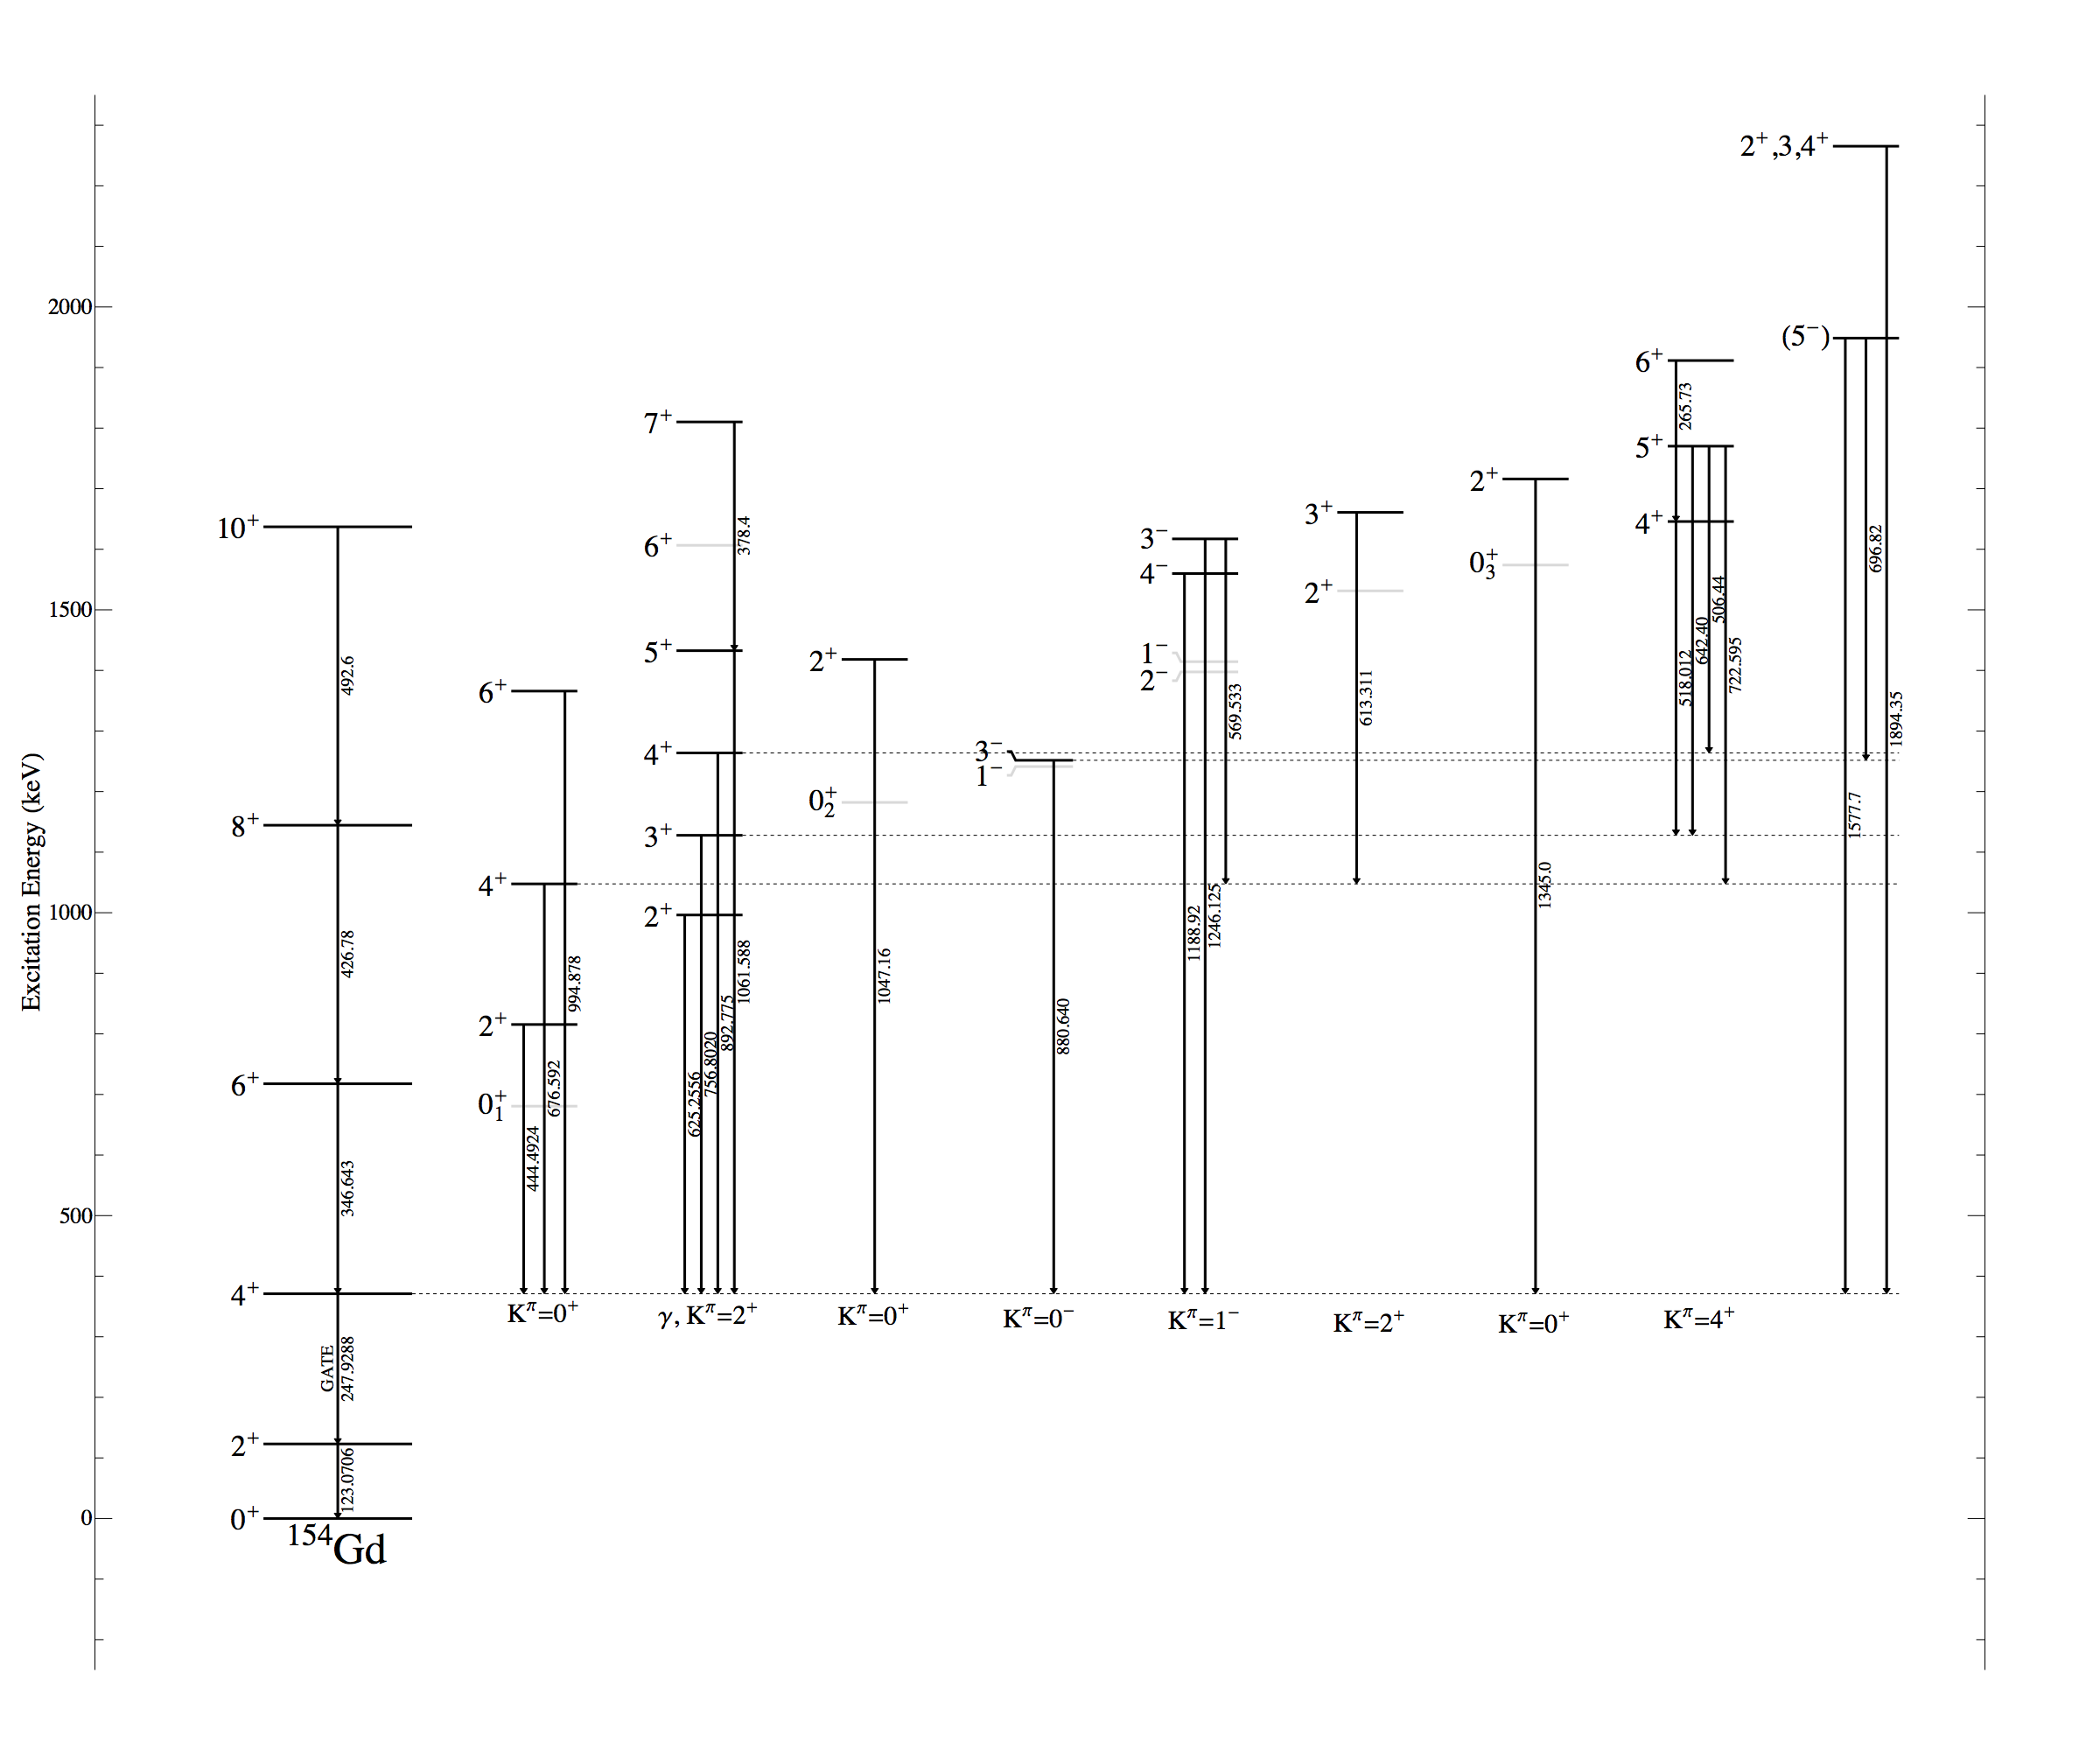
\includegraphics[scale=0.33]{154GdTablesAndFigs/154Gd_4to2.eps}
    \caption*{(a)}
    \label{fig:154_4to2level}
    \end{subfigure}
    \end{figure}
    \end{landscape}
    \begin{figure}
    \ContinuedFloat
    \begin{subfigure}{\textwidth}
    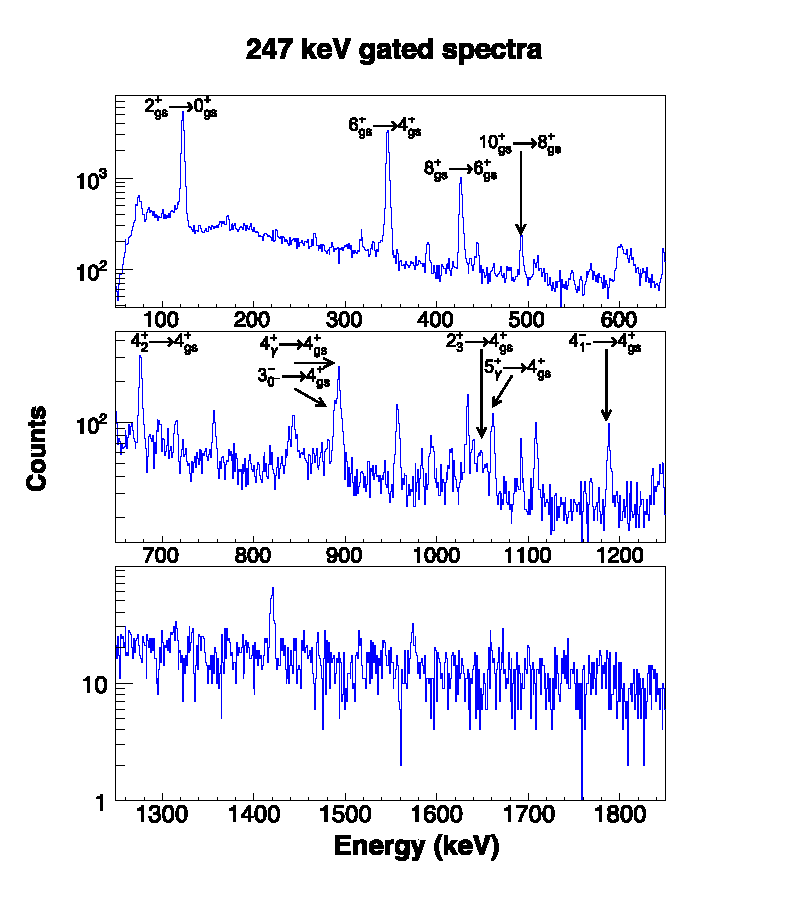
\includegraphics[scale=1.3]{154GdTablesAndFigs/247_gamma.eps}
    \caption*{(b)}
    \label{fig:154_4to2spec}
    \end{subfigure}
\end{figure}}

\afterpage{\clearpage\begin{landscape}
\begin{figure}[!]
    \centering
    \captionlistentry{(a) Level Scheme of $^{154}$Gd. The gate on the $6_{gs}^+\rightarrow 4_{gs}^+$ transition (346 keV) $\gamma$-component in the ground state. The lines shown are in coincidence. The levels are organized by band. The lower levels of the band, unseen by gamma rays in this gate, are in blue. (b) Gamma spectrum gated on 346 keV, corresponding to the $6_{gs}^+\rightarrow 4_{gs}^+$ transition. Several transitions have been labeled, corresponding to the level scheme.}
    \label{fig:154_6to4}
    \begin{subfigure}{1.4\textwidth}
    \caption{\centering \fontsize{10pt}{12pt}Level Scheme of $^{154}$Gd. The gate on the $6_{gs}^+\rightarrow 4_{gs}^+$ transition (346 keV) $\gamma$-component in the ground state. The lines shown are in coincidence. The levels are organized by band. The lower levels of the band, unseen by gamma rays in this gate, are in blue. (b) Gamma spectrum gated on 346 keV, corresponding to the $6_{gs}^+\rightarrow 4_{gs}^+$ transition. Several transitions have been labeled, corresponding to the level scheme.}
    \end{subfigure}
\end{figure}
\clearpage
\begin{figure}
    \ContinuedFloat
    \begin{subfigure}{1.4\textwidth}
    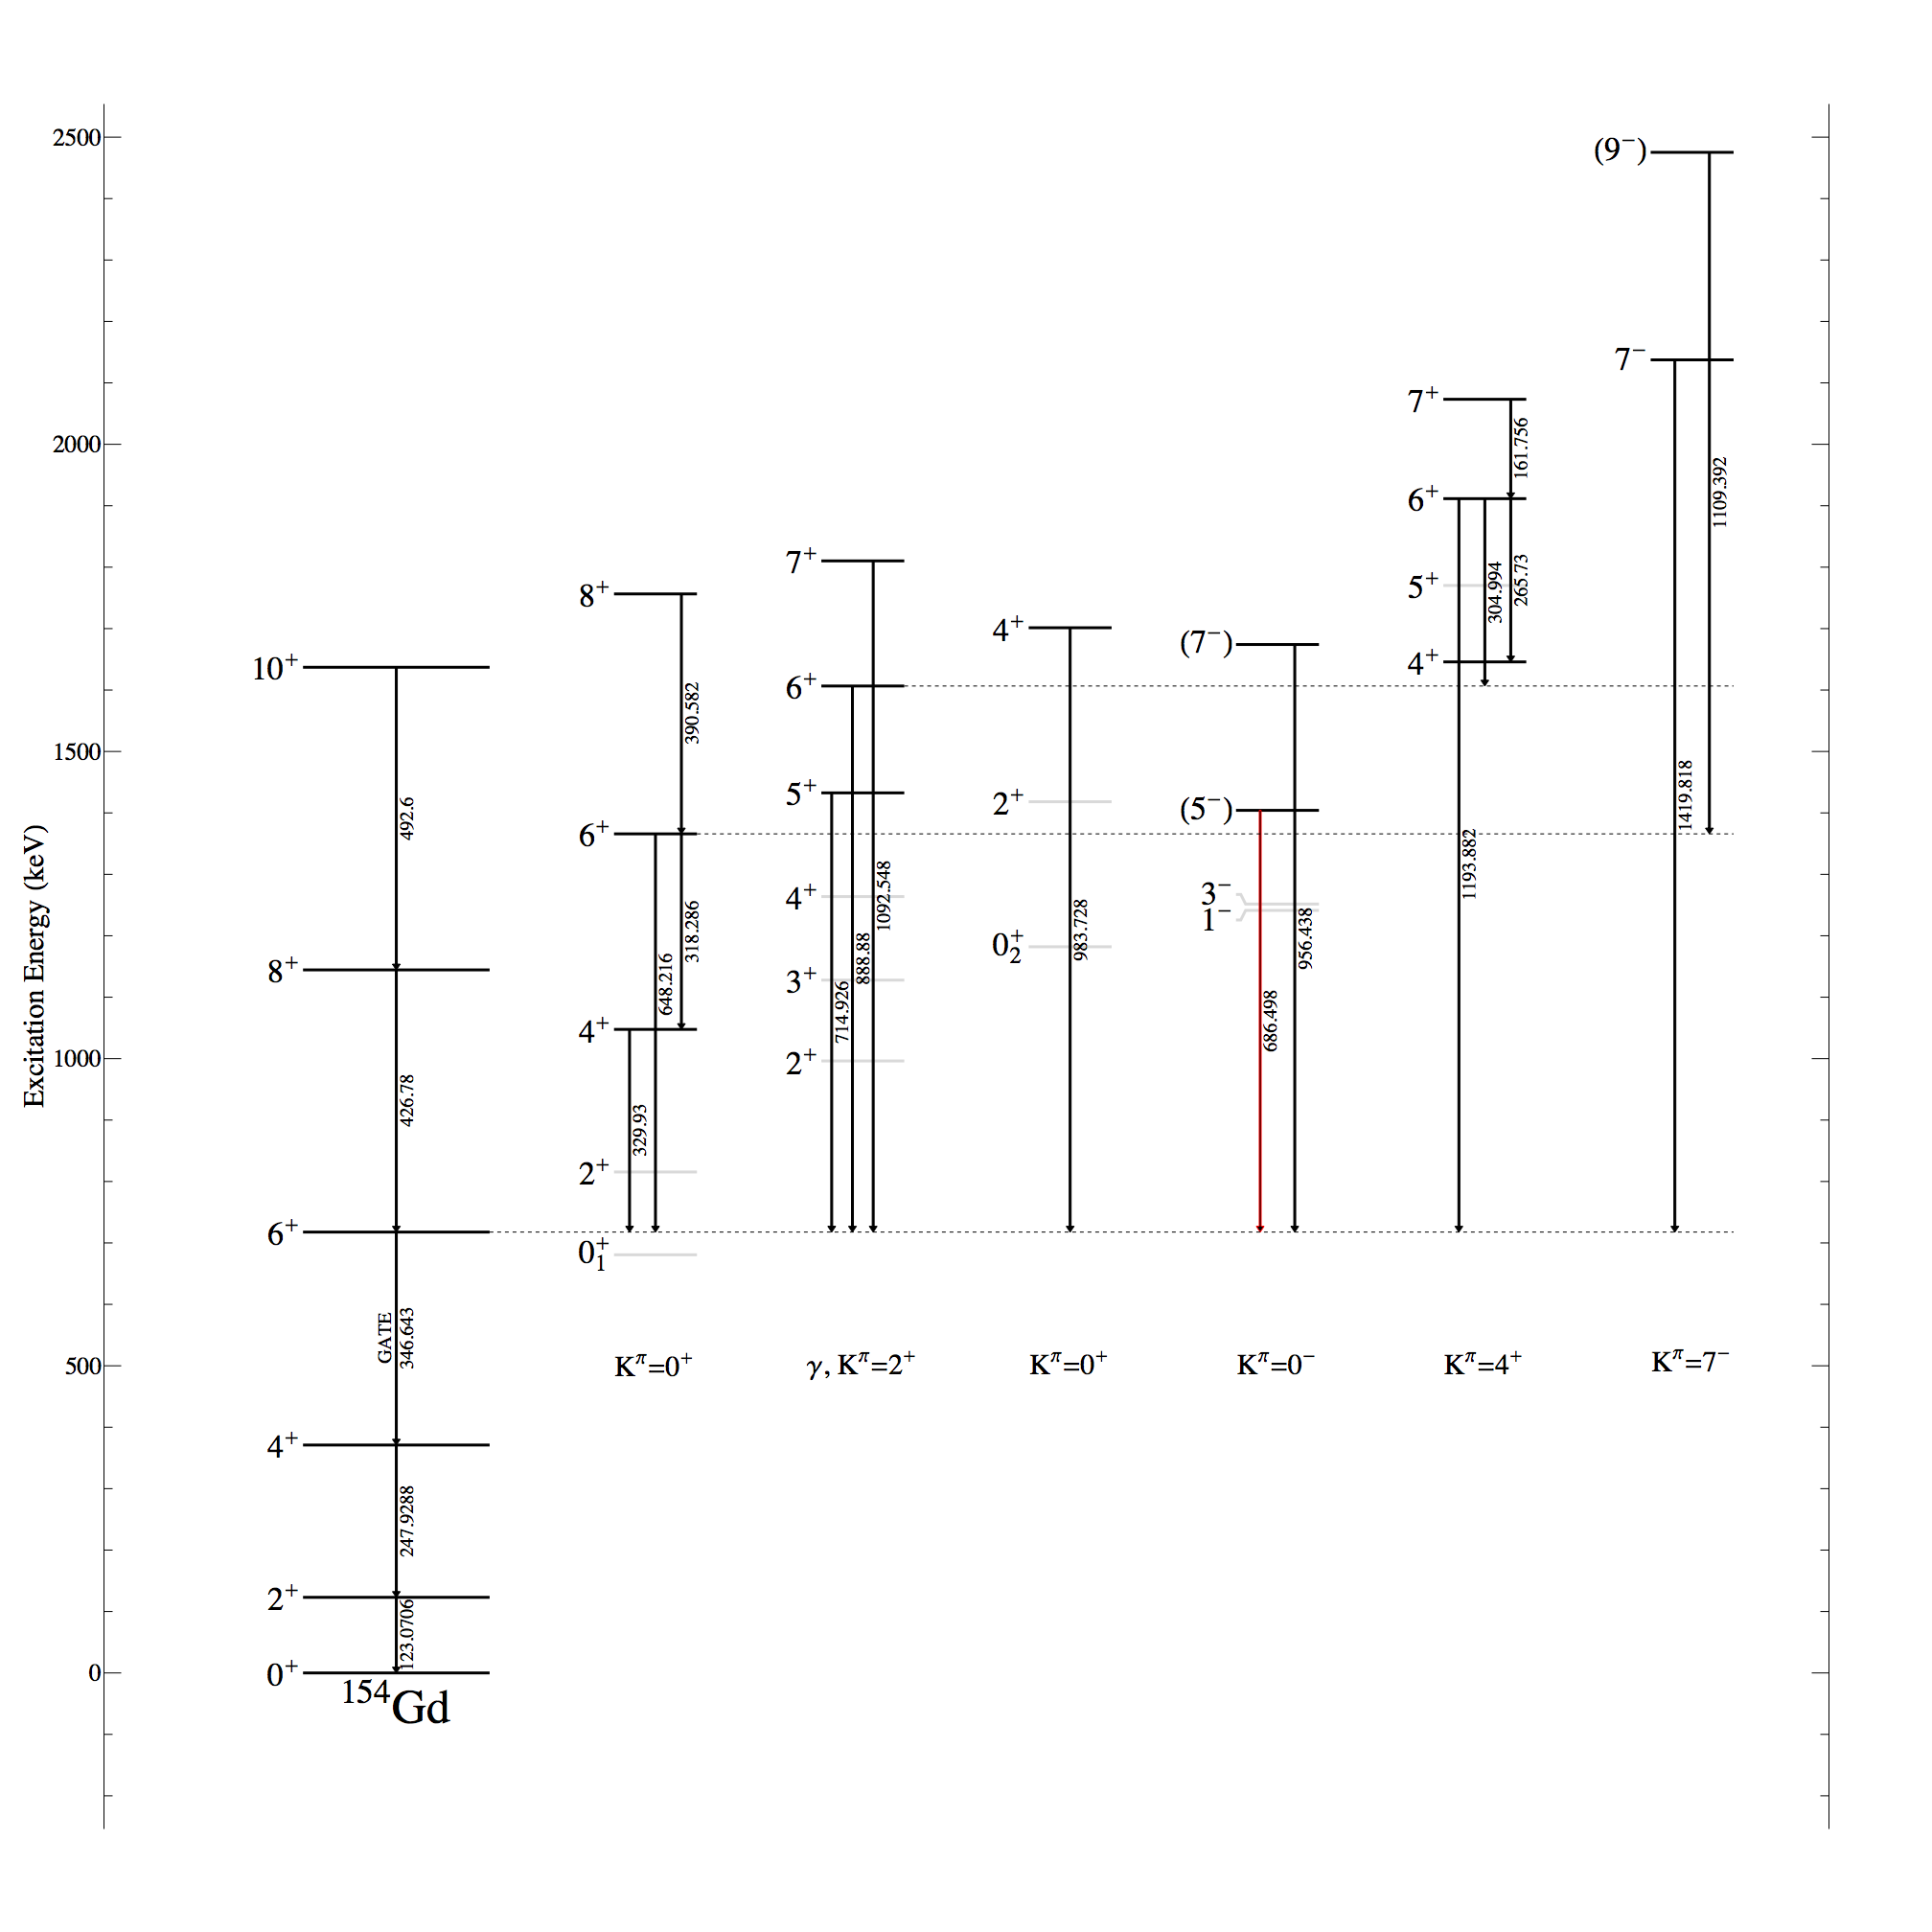
\includegraphics[scale=0.33]{154GdTablesAndFigs/154Gd_6to4.eps}
    \caption*{(a)}
    \end{subfigure}
    \end{figure}
    \end{landscape}
    \begin{figure}
    \ContinuedFloat
    \begin{subfigure}{\textwidth}
    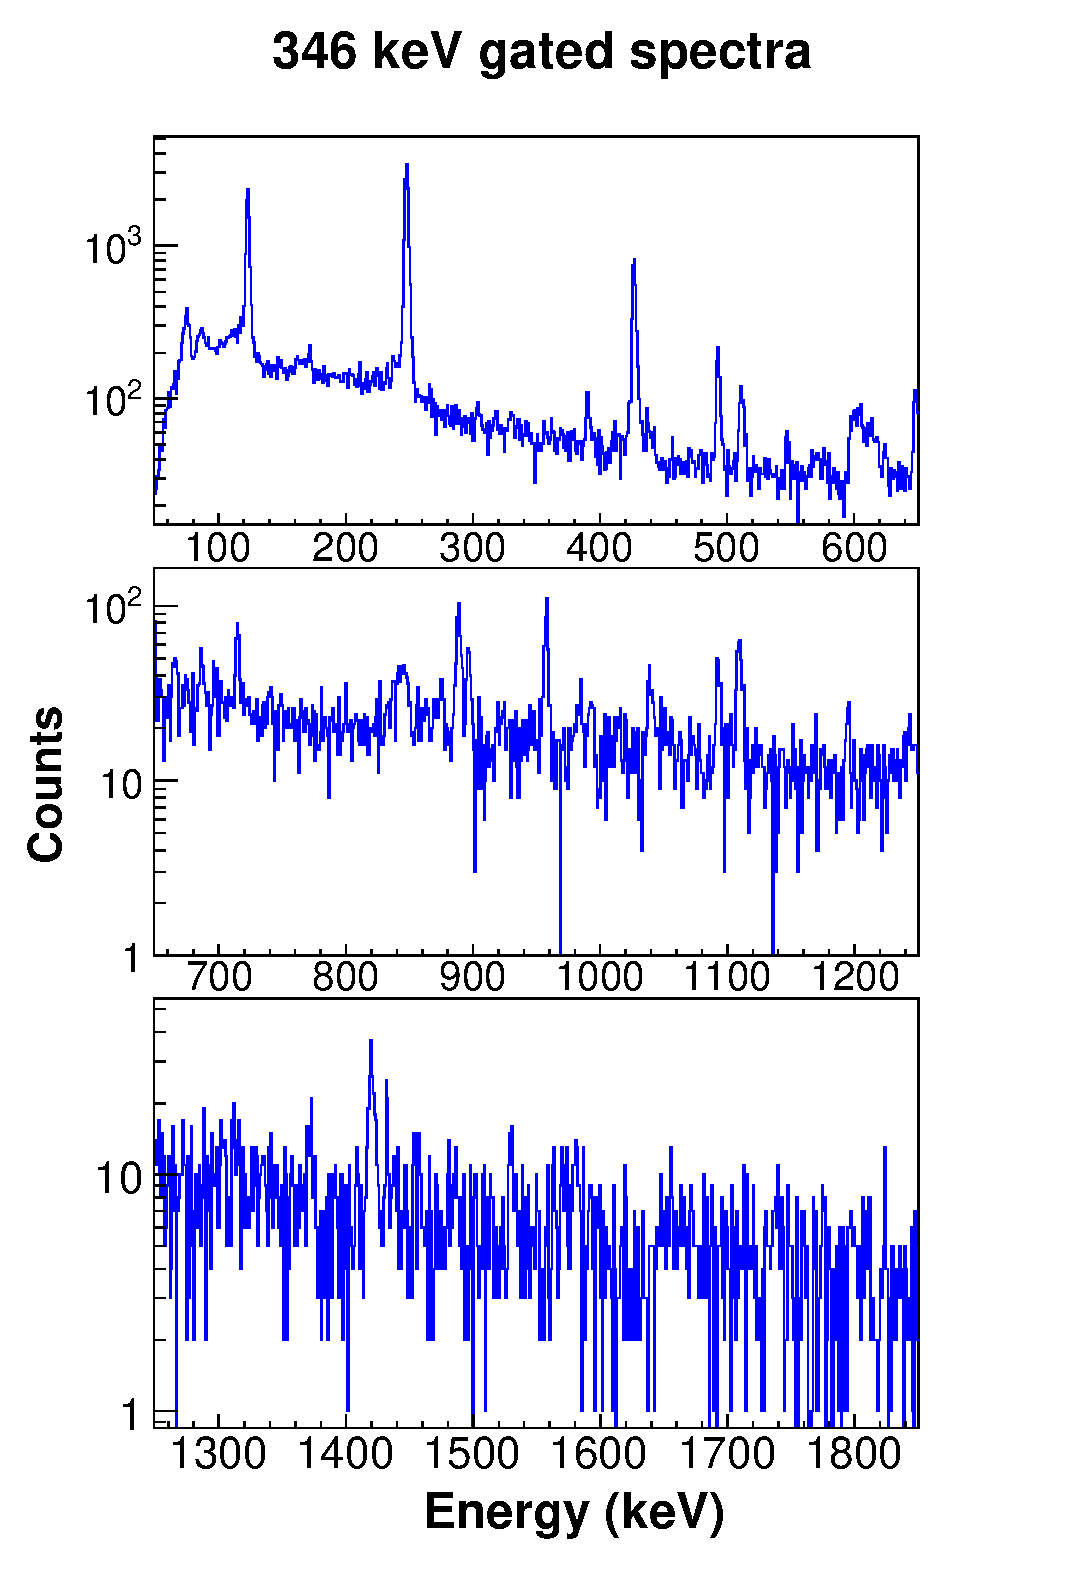
\includegraphics[scale=1.3]{154GdTablesAndFigs/346_gamma.eps}
    \caption*{(b)}
    \label{fig:154_6to4spec}
    \end{subfigure}
\end{figure}}

\afterpage{\clearpage\begin{figure}[!]
    \centering
    \begin{subfigure}{\textwidth}
    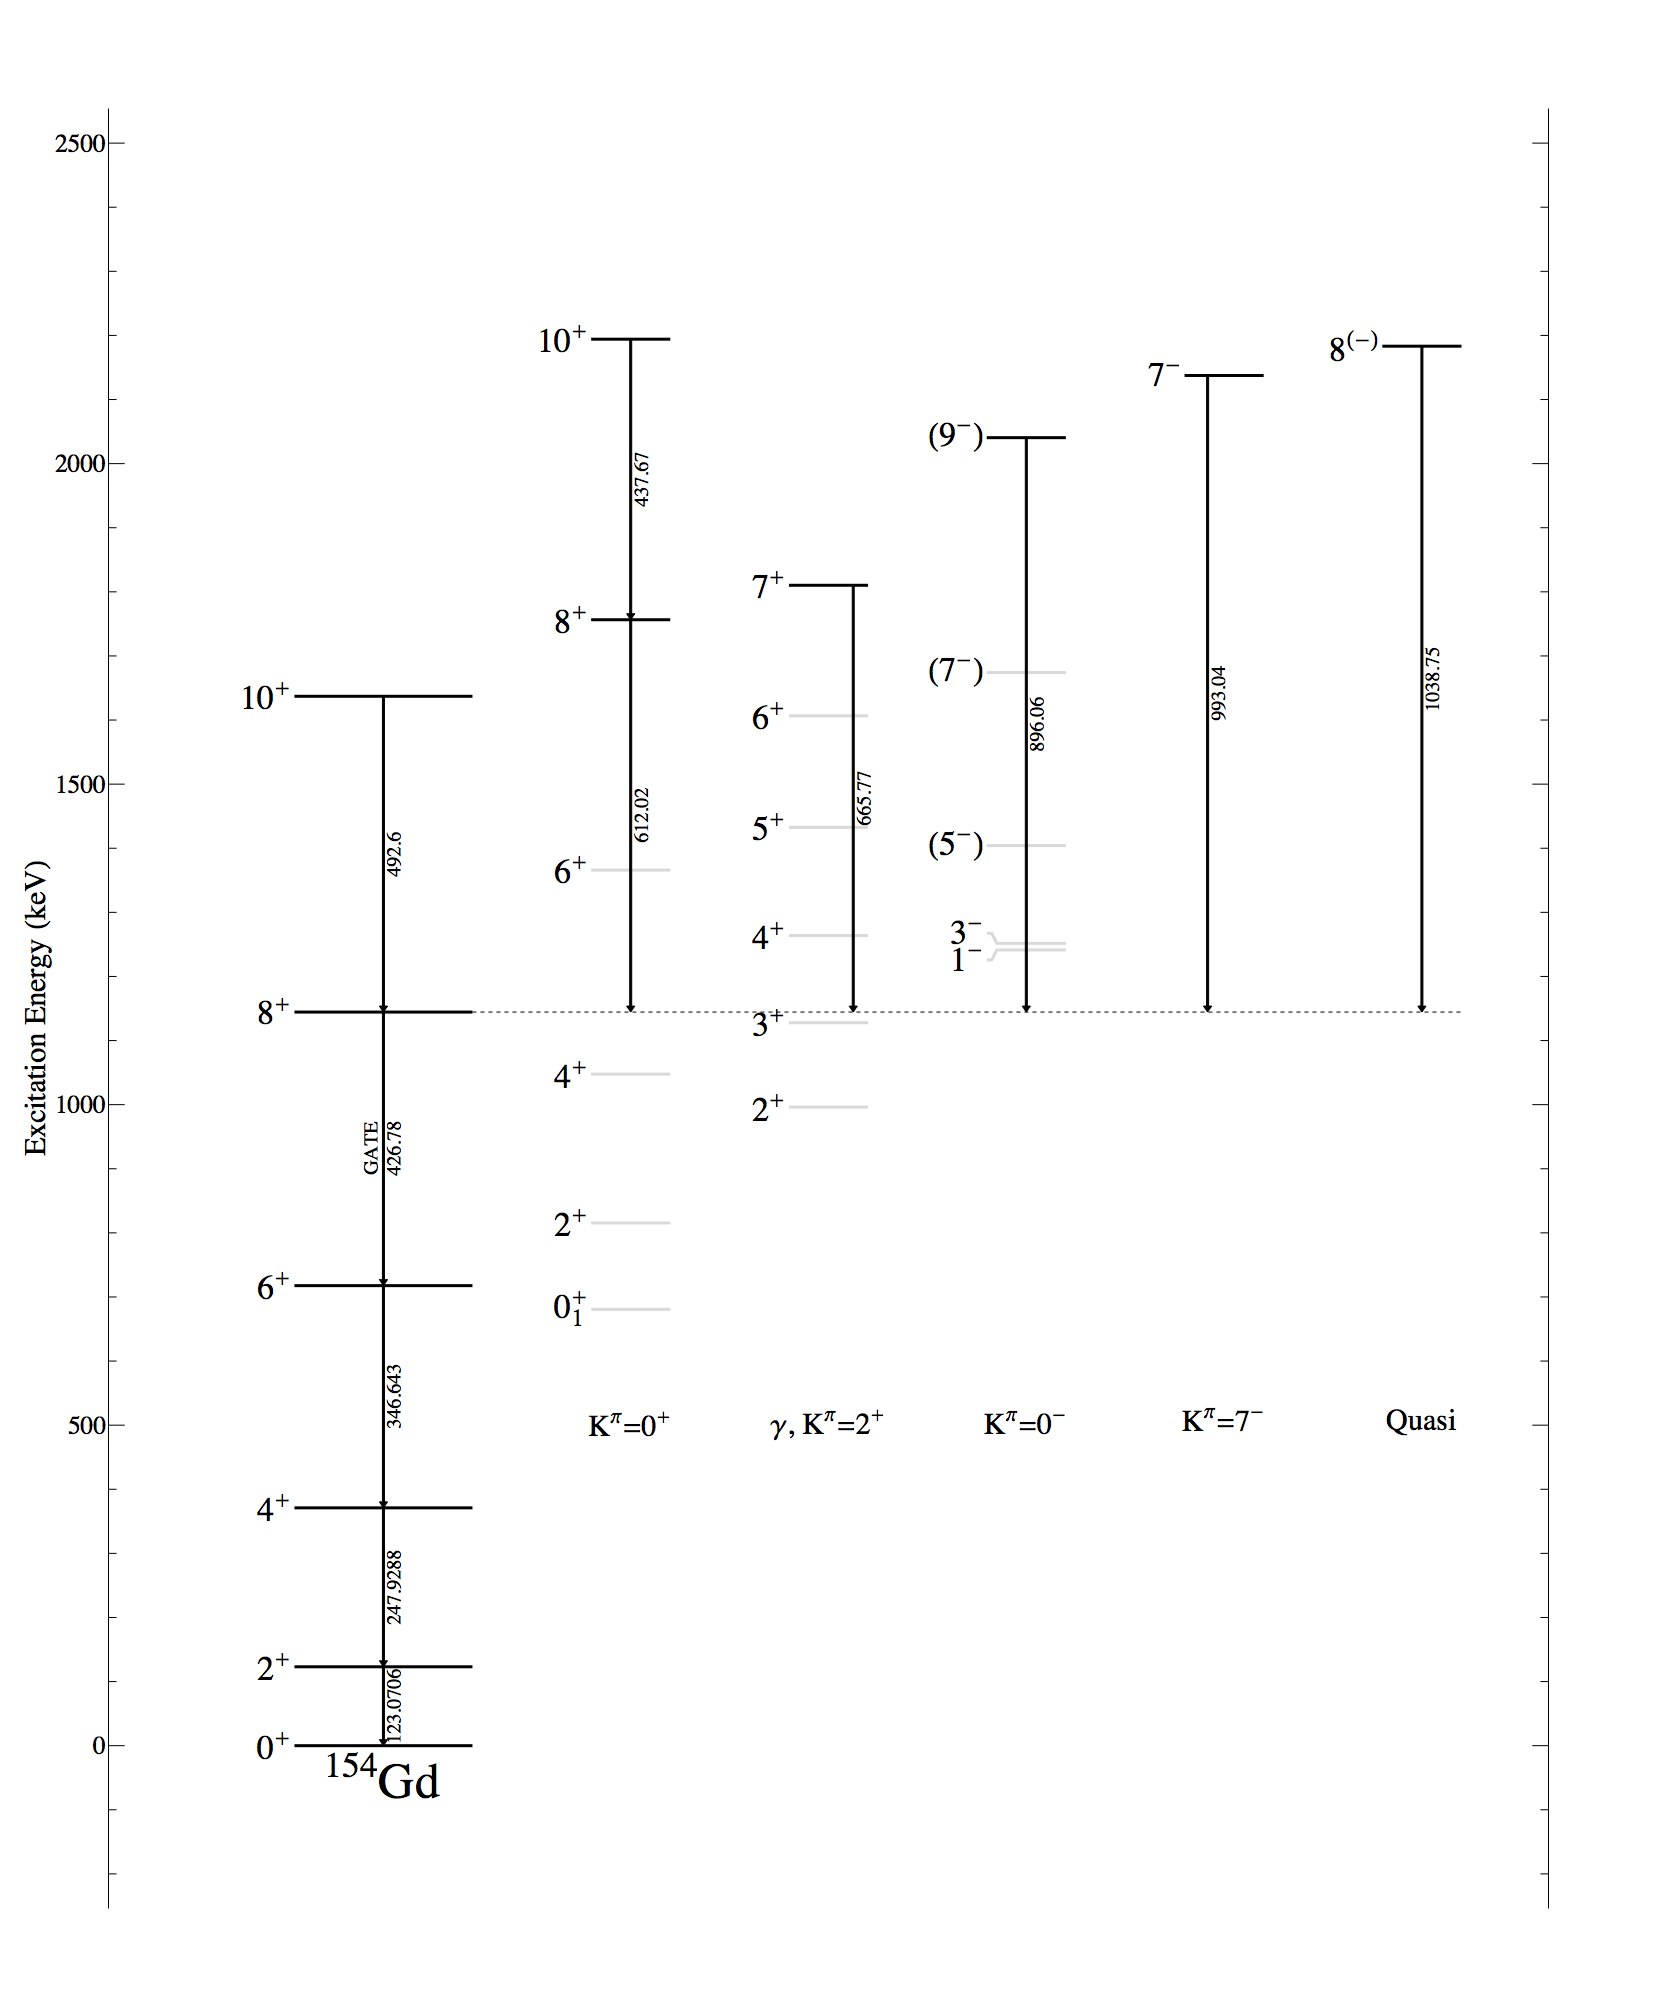
\includegraphics[scale=0.33]{154GdTablesAndFigs/154Gd_8to6.eps}
    \caption{\label{fig:154_8to6level}Level Scheme of $^{154}$Gd. The gamma ray of the $8^+\rightarrow6^+$ transition (426 keV) in the ground state was gated on. It was then compared with the gated spectrum from the gamma ray of the $10^+\rightarrow8^+$ transition (492 keV) in the ground state. Peaks only appearing in the first gate were assumed to go into the $8^+$ state, and assignments were made. Additionally, these peaks were also gated on, to look for cascades leading into the $8^+$ state, which were found in several cases. The levels are organized by band. The lower levels of the band, unseen by gamma rays in this gate, are in gray.}
    \end{subfigure}
    \captionlistentry{Level scheme and spectrum of $^{154}$Gd based on the $8^+\rightarrow6^+$ transition.}
    \label{fig:154_8to6}
    \end{figure}
    \begin{figure}
    \ContinuedFloat
    \begin{subfigure}{\textwidth}
    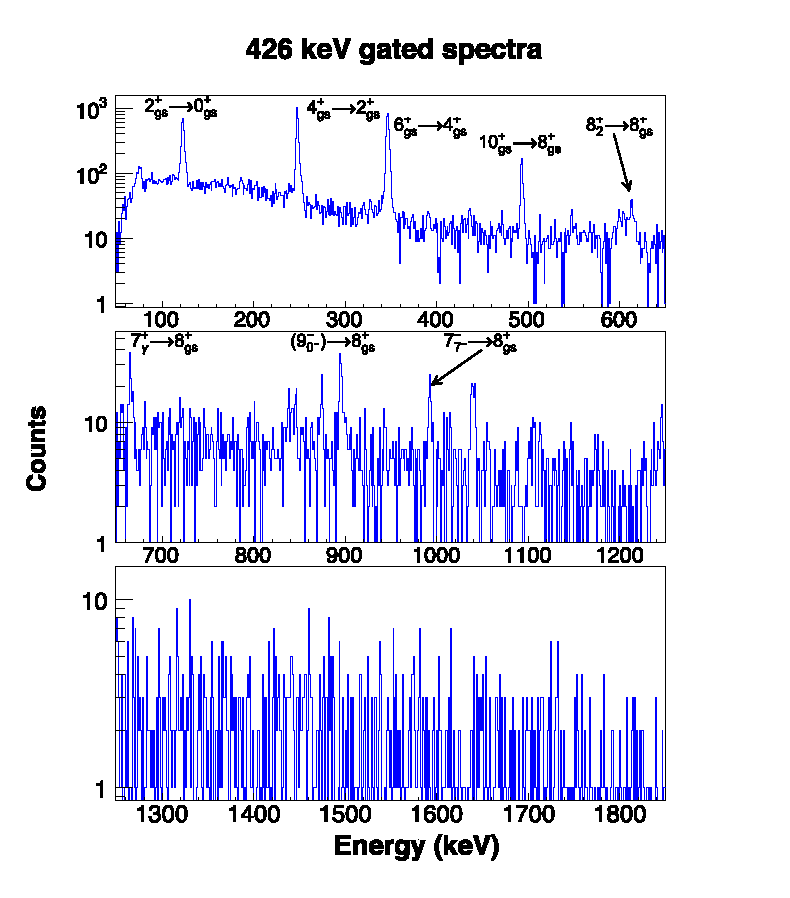
\includegraphics[scale=0.8]{154GdTablesAndFigs/426_gamma.eps}
    \caption{Gamma spectrum gated on 426 keV, corresponding to the $8^+\rightarrow6^+$ transition.}
    \label{fig:154_6to4spec}
    \end{subfigure}
\end{figure}}

\section{Conversion Coefficients from Singles}
\label{sec:154_Conv_Singles}

Conversion coefficients were calculated from the singles spectra. Transitions that could be clearly identified and distinguished are found in Table \ref{tab:154Gd_Single_ICC}. Several transitions with E0 components can be found in Table \ref{tab:154Gd_Single_ICC}. Most of the conversion electrons seen are the $K$-shell electron. These transitions were corrected for angular effects based on the multipolarity of the transition.

Table \ref{tab:154Gd_Single_ICC_Uncorr} conversion coefficients have been left uncorrected in the singles for one of two reasons: either there were multiple known assignments to the gamma-ray energy, or the transition is considered a mixed transition, but no mixing ratio, $\delta$ has been previously measured. For the $3^{+}_{\gamma}\rightarrow 2^+_{0^+_2}$ transition, a mixing ratio, $\delta$, could be calculated by solving the equation
\begin{equation}
    \alpha_{exp}C_{\angle}(\delta)=\frac{1}{1+\delta^2}(\alpha(E2)+\delta^2\alpha(M1))
\end{equation}
where $\alpha_{exp}$ is the uncorrected conversion coefficient, $C_{\angle}(\delta)$ is the angular distribution correction as a function of the mixing ratio, and $\alpha(E2),\alpha(M1)$ are the theoretical conversion coefficients from BrICC\citep{kibedi08:_BRICC}. The upper limit of the experimental value did not yield real values, giving a range of  $-3.46 < \delta < 5.38$.

Table \ref{tab:154Gd_No_Mult_ICC} contains the conversion coefficients that could not be corrected because the transition has no multipole assignment. It contains allowable and reasonable theoretical conversion coefficients to compare the values against, calculated using BrIcc \cite{kibedi08:_BRICC}.

\afterpage{\clearpage\begin{table}
    \centering
    \caption{$^{154}$Gd Internal Conversion Coefficients from Singles}
    \label{tab:154Gd_Single_ICC}
\begin{ThreePartTable}
    \begin{tabular}{c|c|c|c|c|c|c}
        \multicolumn{7}{>{\fontsize{12}{15}}c}{(a)}\\
        \toprule
        $E$ (keV)	&	$J^{\pi}	\rightarrow	J^{\pi}$	&	$E_i$ (keV)	&	$E_f$ (keV)	&	$T_{1/2}$ (fs)	&	Multipolarity	&	$\delta$\\
        \hline
        232.44	&	$4^+_{0^+_2}	\rightarrow	2^+_{0^+_2}$	&	1047.592	&	815.4917	&	7600	&	E2	&	\\
	    &				&		&		&		&		& \\
	    \hline
        329.49	&	$4^+_{0^+_2}	\rightarrow	6^+_{gs}$	&	1047.592	&	717.662	&	7600	&	E2	&	\\
        \hline
        349.89	&	$2^+_{2^+_2}	\rightarrow	0^+_{gs}$	&	1531.305	&	1182.091	&		&	[E2]	&	 \\
        \hline
        416.79	&	$4^+_{0^+_6}	\rightarrow	3^+_{2^+_2}$	&	2080.23	&	1660.903	&		&	(M1)	&	\\
        \hline
        444.19	&	$2^+_{0^+_2}	\rightarrow	4^+_{\gamma}$	&	815.4917	&	370.9998	&	6400	&	E2	&		\\
        \hline
        506.41	&	$5^+_{4^+_1}	\rightarrow	4^+_{\gamma}$	&	1770.187	&	1263.778	&		&	E2	&		\\
        \hline
        515.92	&	$4^+_{4^+_1}	\rightarrow	3^+_{\gamma}$	&	1645.814	&	1127.802	&		&	E2+M1	&	-7 (3)	\\
        \hline
        557.58	&	$0^+_{0^+_2}	\rightarrow	2^+_{gs}$	&	680.6673	&	123.0709	&	4560	&	E2	&		\\
        \hline
        610.71	&	$8^+_{0^+_2}	\rightarrow	8^+_{gs}$	&	1756.49	&	1144.44	&		&	E0+M1+E2	&	-0.69 (14)	\\
	    &				&		&		&		&		&	\\
	    \hline
        676.70	&	$4^+_{0^+_2}	\rightarrow	4^+_{gs}$	&	1047.592	&	370.9998	&	7600	&	E0+M1+E2	&	+2.9 (4)	\\
        \hline
        693.47	&	$2^+_{0^+_2}	\rightarrow	2^+_{gs}$	&	815.4917	&	123.0709	&	6400	&	E2+M1+E0	&	7.5 (4)	\\
        \hline
        873.54	&	$2^+_{\gamma}	\rightarrow	2^+_{gs}$	&	996.2568	&	123.0709	&	950	&	E2+M1+E0	&	-9.4 (4)	\\
        \hline
        889.61	&	$6^+_{\gamma}	\rightarrow	6^+_{gs}$	&	1606.55	&	717.662	&		&	E2+M1	&	$>1.8$	\\
        \hline
        894.40	&	$4^+_{\gamma}	\rightarrow	4^+_{gs}$	&	1263.778	&	370.9998	&		&	E0+M1+E2	&	-3.8 (3)	\\
        \hline
        924.85	&	$4^+_{0^+_2}	\rightarrow	2^+_{gs}$	&	1047.592	&	123.0709	&	7600	&	E2	&	\\
        \hline
        996.33	&	$2^+_{\gamma}	\rightarrow	0^+_{gs}$	&	996.2568	&	0	&	950	&	E2	&	\\
        \hline
        1005.12	&	$3^+_{\gamma}	\rightarrow	2^+_{gs}$	&	1127.8018	&	123.0709	&		&	E2+M1	&	-7.4 (4) \\
        \bottomrule
    \end{tabular}
    \end{ThreePartTable}
\end{table}
\begin{table}
    \begin{ThreePartTable}
        \begin{tabular}{c|c|c|c|c|c}
            \multicolumn{6}{>{\fontsize{12}{15}}c}{TABLE 4.3 (CONTINUED)}\\
            \multicolumn{6}{>{\fontsize{12}{15}}c}{(b)}\\
            \toprule
            $E$ (keV) & Shell &	$\alpha$ (This Work)	&	$\alpha$  (Theory)\citep{kibedi08:_BRICC}	&	$\alpha$ (Spits)\citep{spits96:_154gd} & $\alpha$ (Gono)\citep{gono74:_154gd_e0}		\\
            \hline
            232.44	& K &	0.287	(103) $^{+83}_{-82}$	&	0.0982 (14)	&	0.100 (8)	\\
            &	LM &		0.0450	(46) (13)	&	0.0288 (4)	&		\\
            \hline
            329.49	 & K &	0.1573	(89) (17)	&	0.0352 (5)	&	0.034 (3)	\\
            \hline
            349.89	& K &	0.0298 (8) $^{+8}_{-7}$	&	0.0296 (5)	& $<0.097$ &		\\
            \hline
            416.79	 & K &	0.0334	(47) (6)	&	0.03442 (5)	&	\\
            \hline
            444.19	& K &	0.0525	(32) (6)	&	0.01543 (22)	&	0.014 (1)	\\
            \hline
            506.41	& K &	0.0071	(4) (1)	&	0.01098 (16)	&	0.0100 (11)	\\
            \hline
            515.92	& K & 	0.0069	(5) (1)	&	0.0107 (4)	&	0.0113 (9)	\\
            \hline
            557.58	& K &	0.0486	(42) (6)	&	0.00864 (12)	&	0.009 (1) & 0.0091 (16)	\\
            \hline
            610.71	& K &	0.0258	(10) (7)	&	0.0110 (6)	& &	0.053 (7)	\\
            		& L &	0.0167	(9) (4)	&	0.00158 (7)	&		\\
            \hline
            676.70	& K &	0.0283	(4) (10)	&	0.00593 (17)	&	0.0460 (46) & 0.040 (7)	\\
            \hline
            693.47	& K &	0.0017	(2) (1)	&	0.00522 (8)	&	0.0421 (4)	\\
            \hline
            873.54	& K &	0.0021	(3)	(1) &	0.00311 (5)	&	0.0035 (1)	\\
            \hline
            889.61	& K &	0.0043	(6) (2)	&	0.00349 (5)	&	0.0033 (2)	\\
            \hline
            894.40	& K &	0.0019	(2) (1)	&	0.00307 (5)	&	0.0039 (3)	\\
            \hline
            924.85	& K &	0.0033	(9) (1)	&	0.00273 (4)	&	0.0031 (1)	\\
            \hline
            996.33	& K &	0.0021	(4) (1)	&	0.00234 (4)	&	0.0025 (1)	\\
            \hline
            1005.12	& K &	0.0019	(1) (1)	&	0.00233 (4)	&	0.0024 (1)	\\
            \bottomrule
        \end{tabular}
        \begin{tablenotes}[para]
            Table \ref{tab:154Gd_Single_ICC}: A list of conversion coefficients from $^{154}$Gd. Table (a) lists transition information. Multipolarities and mixing ratios were taken from the nuclear data sheets\citep{reich09:_nds_154}. Table (b) lists the conversion coefficients. Unless otherwise stated, the $\alpha$ values are $\alpha_K$. An angular distribution correction has been applied based on multipolarities for pure transitions, and those with known mixing ratios. The first error is statistical, the second is systematic. Numbers are compared with Spits et al.\citep{spits96:_154gd} and Gono et al.\citep{gono74:_154gd_e0} The starred value was used as an absolute calibration of the conversion electron detector in the Gono work. The bands for each level are listed as subscripts.
        \end{tablenotes}
\end{ThreePartTable}
\end{table}
}

\afterpage{\clearpage\begin{sidewaystable}
\footnotesize
    \begin{longtable}{c|c|c|c|c|c|c|c|c|c|c}
        \caption{Uncorrected $^{154}$Gd Internal Conversion Coefficients from Singles}
        \label{tab:154Gd_Single_ICC_Uncorr}\\
        \toprule
        $E$ (keV)	&	$J^{\pi}	\rightarrow	J^{\pi}$	&	$E_i$ (keV)	&	$E_f$ (keV)	&	Multipolarity	&	$\delta$ & Shell	&	$\alpha$ (This Work)				&	$\alpha$  (Th)	&	$\alpha$ (Spits) & $\alpha$ (Gono)		\\
        \hline
        \endfirsthead
        \caption[]{Uncorrected $^{154}$Gd Internal Conversion Coefficients from Singles}\\
        \toprule
        $E$ (keV)	&	$J^{\pi}	\rightarrow	J^{\pi}$	&	$E_i$ (keV)	&	$E_f$ (keV)	&	Multipolarity	&	$\delta$ & Shell	&	$\alpha$ (This Work) 			&	$\alpha$  (Th)	&	$\alpha$ (Spits) & $\alpha$ (Gono)	\\
        \hline
	    \endhead
	    \hline
        198.311	&	$3^-	\rightarrow	2^+$	&	1617.123	&	1418.16		&	[E1]	&		& K &	0.0842	(26) (19)	&	0.0393 (6)	&		\\
	    &	$(9)^+	\rightarrow	(8)^+$	&	2453.29	&	2254.12		&		&		&					&		&	&	\\
	    \hline
        313.21	&	$3^+	\rightarrow	2^+$	&	1127.802	&	815.492		&	[M1,E2]	&	 & K	&	0.0805	(47) (20)	&		&		\\
        \hline
        641.92	&	$5^+	\rightarrow	3^+$	&	1770.187	&	1127.8018		&	M1,E2	&		& K &	0.0303 (7) (8)	&		&	0.0086 (8)	\\
        648.951	&	$6^+	\rightarrow	6^+$	&	1365.87	&	717.662		&	E0+M1+E2	&	+1.30 (20)	&		&	0.0079 (5)	&	& 0.039 (7)	\\
        \hline
        715.198	&	$2^+	\rightarrow	2^+$	&	1531.305	&	815.492		&	E0+M1+E2	&		& K &	0.0199	(5) (5)	&		&	0.0070 (5)	\\
	    &				&		&			&		&		& L &	0.0041	(4) (1)	&		&		\\
	    \hline
        1061.59	&	$0^+	\rightarrow	2^+$	&	1182.091	&	123.0709		&	E2	&		& K &	0.0022	(3) (1)	&	0.0021 (1)	&		\\
	    &	$5^+	\rightarrow	4^+$	&	1432.588	&	370.9998		&	E2+M1	&	$-4.3^{+12}_{-26}$	&			&	0.0021 (1)	&	0.0019 (4) & &	\\
        \bottomrule
    \end{longtable}
    \item{Table \ref{tab:154Gd_Single_ICC_Uncorr}: A list of conversion coefficients from $^{154}$Gd. Multipolarities and mixing ratios were taken from NNDC. Unless otherwise stated, the $\alpha$ values are $\alpha_K$. No angular distribution correction has been applied, either due to unknown mixing ratios, or multiple assignments of the gamma-ray. None of the above transitions have known half-lives. The first error is statistical, the second is systematic. Numbers are compared with Spits et al.\citep{spits96:_154gd} and Gono et al.\citep{gono74:_154gd_e0}}
\end{sidewaystable}}

\afterpage{\clearpage\begin{landscape}
\begin{table}
    \centering
    \caption{$^{154}$Gd Internal Conversion Electrons without Assigned Multipolarities}
    \label{tab:154Gd_No_Mult_ICC}
\begin{ThreePartTable}
        \centering
    \begin{tabular}{>{\footnotesize}c|>{\footnotesize}c|>{\footnotesize}c|>{\footnotesize}c}
        \multicolumn{4}{>{\fontsize{12}{15}}c}{(a)}\\
        \toprule
        $E$ (keV) & $J_i\rightarrow J_f$	& $E_i$ (keV) 	& $E_f$ (keV) \\
	    \hline
	    266.37	&	$6^+_{4^+_1}	\rightarrow	4^+_{4^+_1}$	&	1911.544	&	1645.814 \\ \hline
	    303.89	&	$(7^+)_{4^+_1}	\rightarrow	5^+_{4^+_1}$	&	2073.30	&	1770.187 \\ \hline
	    318.382	&	$6^+_{0^+_2}	\rightarrow	4^+_{0^+_2}$	&	1365.87	&	1047.592	\\
	    &		&		&		\\  \hline
	    379.55	&	$7^+_{\gamma}	\rightarrow	5^+_{\gamma}$	&	1810.21	&	1432.588 \\ \hline
        433.12	&	$4^+_{0^+_6}	\rightarrow	4^+_{4^+_1}$	&	2080.23	&	1645.814	\\ 
        	&	&	&	\\ \hline
        687.05	&	$(5^-)_{0^-} \rightarrow 6^+_{gs}$		&	1404.16	&	717.662 \\ \hline
        722.64	&	$5^+_{4^+_1}	\rightarrow	4^+_{0^+_2}$	&	1770.187	&	1047.592 \\
        &	&	&	\\ \hline
        1033.91	&	$3^-	\rightarrow	4^+_{0^+_2}$	&	2080.791	&	1047.592 \\
        \bottomrule
    \end{tabular}
\end{ThreePartTable}
\end{table}

\begin{table}
    \centering
\begin{ThreePartTable}
    \centering
    \begin{tabular}{>{\footnotesize}c|>{\footnotesize}c|>{\footnotesize}c|>{\footnotesize}c|>{\footnotesize}c|>{\footnotesize}c|>{\footnotesize}c|>{\footnotesize}c}
        \multicolumn{7}{>{\fontsize{12}{15}}c}{TABLE 4.5 (CONTINUED)}\\
        \multicolumn{7}{>{\fontsize{12}{15}}c}{(b)}\\
        \toprule
        &	& \multicolumn{2}{>{\footnotesize}c|}{$\alpha$ (This Work) } & \multicolumn{3}{>{\footnotesize}c|}{Theory\citep{kibedi08:_BRICC}}	& 	\\ 
        $E$ (keV)	& Shell & 	Uncorrected & Corrected 	& $\alpha$(M1) & $\alpha$(E2) & $\alpha$(E1) &	$\alpha$ (Spits)\citep{spits96:_154gd}	\\
	    \hline
	    266.37	& K &	0.2074	(74) (50) & 0.1684 (60) (41) &  & 0.0654 (10) & & \\ \hline
	    303.89	& K &	0.1183	(40) $^{+30}_{-29}$  & 0.0954 (32) $^{+24}_{-23}$ & & 0.0444 (7) & & \\ \hline
	    318.382	& K &	0.0736	(18) (18)  & 0.0600 (15) (15) & & 0.0388 (6) & &\\
	    		& L & 	0.0371	(12) (9) & 0.0301 (10) (7)	& & 0.00892 (13) & &	\\  \hline
	    379.55	& K & 	0.1120	(60) (31) & 0.0903 (48) (25)&  & 0.0236 (4) & & \\ \hline
        433.12	& K &	0.0571	(42) (15) & [M1] 0.0777 (57) (20) & 0.0310 (5) & 0.01650 (24) &	& 0.0220 (45)\\ 
        	&	& & [E2] 0.0351 (26) (9) & & &	& \\ \hline
        687.05	& K & 0.3538 (116) (90) & 0.6435 (211) (163)	& & & 0.00203 (3) &\\ \hline
        722.64	& K		&	0.0166	(12) (42) & [M1] 0.0107 (8) (27)	& 0.00856 (12) & 0.00468 (7) & &		\\
        &	& &  [E2] 0.0185 (13) (47) & & &	& \\ \hline
        1033.91	& K	&	0.0015	(4) (1) & 0.0028 (7) (2)	& & & 0.000916 (13) &	\\
        \bottomrule
    \end{tabular}
\begin{tablenotes}[para]
    Table \ref{tab:154Gd_No_Mult_ICC}: A list of conversion coefficients from $^{154}$Gd without known multipolarities. Table (a) lists transition information. Table (b) lists the conversion coefficients and theoretical values. As a result, an angular distribution correction term cannot be applied to compare with theory, except in the case of pure multipoles. None of the above transitions have known half-lives. The first error is statistical, the second is systematic. Numbers are compared with theoretical coefficients for allowed and reasonable polarities, as well as results from Spits et al. \cite{spits96:_154gd} The bands for each level are listed as subscripts. The $3^-$ for $E=1033.91$ keV has no band placement.
    \end{tablenotes}
\end{ThreePartTable}
\end{table}
\end{landscape}}   

In Table \ref{tab:154Gd_Single_ICC}, there are several conversion coefficients that are high, not only compared to theory, but compared to previous measurements (232, 329, 444, and 557 keV). For the 232 keV transition, the large error hints at a lack of statistics.  For the other three transitions, the transition indicates a change from smaller to larger $J^{\pi}$. The angular distribution correction for such transitions is less than 1, inflating the value. This may be an indication the angular distribution correction is not wholly accurate. Further, due to these values being from singles data, unknown contaminants to the electron spectrum cannot be ruled out. While these transitions were identified clearly and separably, low-intensity gamma-rays may have not have had enough statistics to appear in gated spectra. There are also three transitions that are lower than the theoretical values (515, 873 and 894 keV). In all of these cases, $\delta$ is negative. Finally, there are several $J^{\pi}\rightarrow J^{\pi}$ transitions seen in the singles. For the $4^+_{0^+_2}\rightarrow 4^+_{gs}$ between the first excited $0^+$ band and the ground state band at 676 keV, there is clearly an E0 component, although not as big at that seen by Spits or Gono \cite{spits96:_154gd, gono74:_154gd_e0}. It is a similar situation for the $8^+_{0^+_2}\rightarrow 8^+_{gs}$ at 610 keV compared to Gono. Additionally, there is a $6_{\gamma}^+\rightarrow 6^+_{gs}$ transition at 889 keV that is higher than number from Spits and the theoretical conversion coefficient. The $4^+_{\gamma}\rightarrow 4^+_{gs}$ was also found in gating, as will be discussed in the next section.

In Table \ref{tab:154Gd_Single_ICC_Uncorr}, the $2^+_{2^+_2}\rightarrow 2^+_{0^+_2}$ transition at 715 keV appears to have a large E0 component. This transition is examined in the next section. For the two entangled transitions around 645 keV, the $6^+_{0^+_2}\rightarrow 6^+_{gs}$ transition is likely the dominant contribution, as the measured value in the singles is in good agreement with the measured value in the gated data, see Table \ref{tab:154Gd_6_to_6}. Two separate $\alpha$ values are listed in this part of Table \ref{tab:154Gd_Single_ICC_Uncorr}, as the gamma-rays were separable, but the conversion electron peaks were not.

In Table \ref{tab:154Gd_No_Mult_ICC}, the $4^+_{0^+_6}\rightarrow 4^+_{4^+_1}$ transition at 433 keV either indicates a mixed transition with an E0 component. The angular correction for a pure E2 transition would make the conversion coefficient approximately double the theoretical conversion coefficient from BrICC \citep{kibedi08:_BRICC}. This angular correction is the largest correction that can made. Mixed component angular corrections result in values larger than the theoretical M1 transition. Together, this points toward an E0 component to the transition. Unfortunately, this transitions could not be found in gates, as the levels are too high in energy to be populated significantly enough for gates.

\section{$J^{\pi}\rightarrow J^{\pi}$ Transitions}
\label{sec:154_J2J}

\subsection{$0^{+}\rightarrow 0^{+}$ Identification and Population}

With the large number of $0^+$ states in $^{154}$Gd, our first priority was to identify which bands were populated. Table \ref{tab:0plus_154} contains a list of $0^+$ states from Meyer et al, with indications as to which $0^+$ have been observed outside of the discovery paper, and which have been previously observed in the reaction used in this work \cite{meyer06:_zeroplus}.

\begin{table}
    \centering
    \begin{ThreePartTable}
        \caption{$0^+$ States in $^{154}$Gd}
        \label{tab:0plus_154}
    \begin{tabular}{c|c|c|c}
        Energy (keV) & Seen Previously \citep{meyer06:_zeroplus} & Seen in $(\alpha,2n)$ & Seen in This Work  \\
        \toprule
        0 & $\times$ & $\times$ & $\times$\\
        680.4(3) & $\times$ & $\times$ & $\times$\\
        1181.9(3) & $\times$ &  & $\times$\\
        1352.9(3) & & &\\
        1497.7(3) & & &\\
        1573.7(3) & $\times$ &  & $\times$\\
        1650.6(4) & $\times$ &  & $\times$\\
        1836.7(4) & & &\\
        1899.3(4) & & &\\
        1942.9(4) & & &\\
        2039.8(4) & & &\\
        2299.9(5) & $\times$ & &\\
        2485.1(5) & & &\\
        2585.3(5) & & &\\
        2744.5(5) & $\times$ & &\\
        2855.0(5) & $\times$ & &\\
        \bottomrule
    \end{tabular}
        \begin{tablenotes}[para]
        Table \ref{tab:0plus_154}: A list of all $0^+$ states in $^{154}$Gd. All the states listed were seen in Meyer et al, a $(p,t)$ experiment\citep{meyer06:_zeroplus}. $0^+$ states above approximately 2184 keV would not be seen in this experiment, the energy of the $12^+$ ground state, as that is the energy cut off in the nucleus for state population, discussed in the text. The levels seen in this exceed previous $(\alpha,2n)$ experiments and agree with the levels seen in Spits \citep{spits96:_154gd}. Until Spits, there was no known spectroscopy for the 1182, 1573 and 1650 keV states, having only been seen previously in $(p,t)$ and $(t,p)$ experiments. No $(\alpha,2n)$ experiments with $\gamma-\gamma$ coincidence, looking for such levels have been run since Spits et al was published.
        \end{tablenotes}
\end{ThreePartTable}
\end{table}

Many of the states were left unseen in this work as is to be expected. We have seen all states that were observed previously in $(\alpha,2n)$ experiments, in addition to three other $0^+$ excited states. The energy of the $12^+$ in the ground state band, 2184.69 keV, is the rough cut off for populating states. The levels seen in this work exceed previous $(\alpha,2n)$ experiments and agree with the levels seen in Spits et al, a thermal neutron capture experiment\citep{spits96:_154gd}. Until Spits, there was no known spectroscopy for the 1182, 1573 and 1650 keV states, having only been seen previously in $(p,t)$ and $(t,p)$ experiments. No $(\alpha,2n)$ experiments with $\gamma-\gamma$ coincidence, looking for such levels have been run since Spits et al was published in 1996. The energies of the $0^+\rightarrow0^+$ transitions from these states are marked in the electron singles in Figure \ref{fig:154_e_singles}. The most prominent is the $0^+_{2}\rightarrow0^+_{gs}$ transition. The $0^+_{7}\rightarrow0^+_{3}$ transition is at the energy of the $10^+_{gs}\rightarrow8^+_{gs}$ K-electron energy, and the $0^+_{6}\rightarrow0^+_{3}$ transition is between the $8^+_{gs}\rightarrow6^+_{gs}$ L and M electron energies. The $0^+_{7}\rightarrow0^+_{6}$ transition may be present, but sits on the low energy tail of the $2^+_{gs}\rightarrow0^+_{gs}$ L electron peak. To obtain information in these areas, and for possible $J^{\pi}\rightarrow J^{\pi}$ transitions, energy gates were used. A full list of gates and spectra can be found in Appendix \ref{chap:154_spectra}.

\begin{figure}
    \centering
    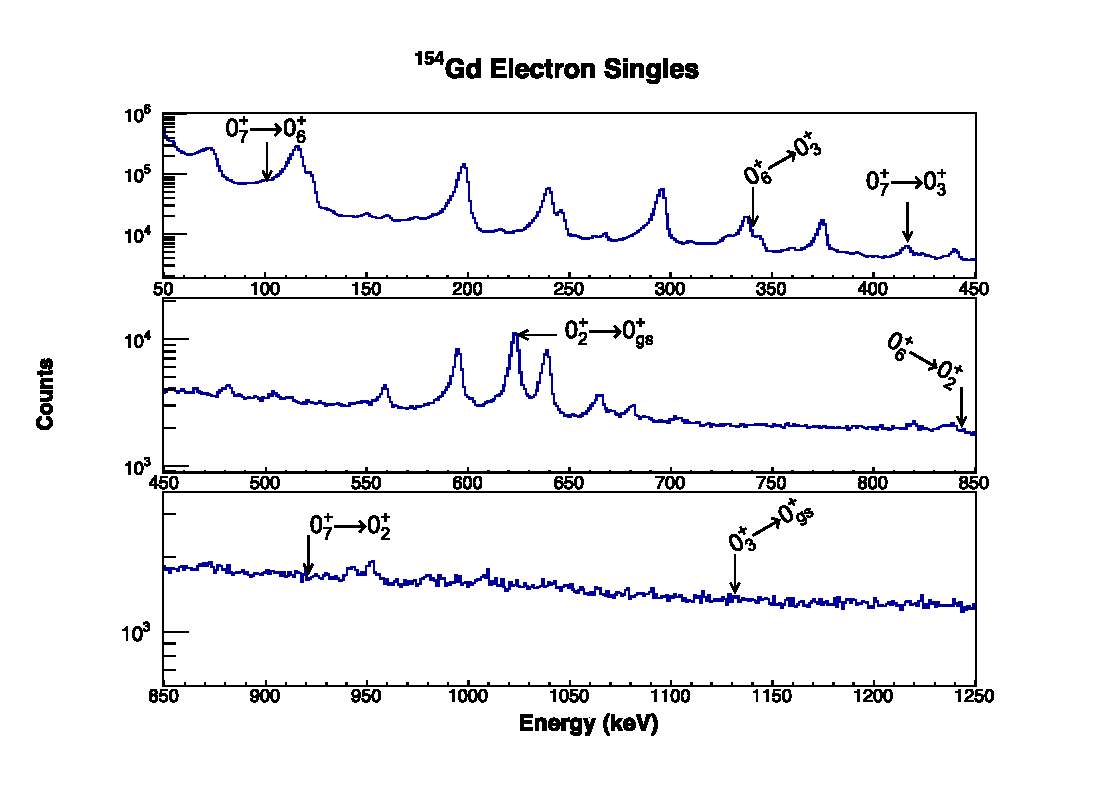
\includegraphics[scale=0.8]{154GdTablesAndFigs/154Gd_Singles_Electron_Label.eps}
    \caption{Electron singles for $^{154}$Gd. The energies of transitions between $0^+$ states are marked in the plot. The most prominent is the $0^+_{2}\rightarrow0^+_{gs}$ transition. The $0^+_{7}\rightarrow0^+_{3}$ transition is at the energy of the $10^+_{gs}\rightarrow8^+_{gs}$ K-electron energy, and the $0^+_{6}\rightarrow0^+_{3}$ transition is between the $8^+_{gs}\rightarrow6^+_{gs}$ L and M electron energies. The $0^+_{7}\rightarrow0^+_{6}$ transition may be present, but sits on the low energy tail of the $2^+_{gs}\rightarrow0^+_{gs}$ L electron peak.}
    \label{fig:154_e_singles}
\end{figure}

\subsection{$J^{\pi}\rightarrow J^{\pi}$ Transitions}

After identification of the bands and transitions, gates were put on the outgoing and incoming transitions of states of interest, namely even-$J^{+}$ states. Gates on incoming transitions did not have enough statistics to extract data on transitions of interest from the resulting spectra. However, gates on outgoing transitions allowed enough statistics to look for transitions from states of the same $J^{\pi}$. In many cases, two separate outgoing transition gates could be used to look at the same state. To look for these transitions of interest, other electron peaks, namely those of the ground state band, were subtracted from the regions of interest as described in Section \ref{sec:upper_limit}. This subtraction technique causes the results to be treated as limits. Tables \ref{tab:154Gd_0_to_0} - \ref{tab:154Gd_6_to_6} are the tabulated results. Where previous measurements have been taken, they are been listed. Additionally, the theoretical conversion coefficients have been listed for $M1$ and $E2$ transitions, as taken from BrIcc \cite{kibedi08:_BRICC}.

\afterpage{\clearpage\begin{sidewaystable}
    \begin{longtable}{c|c|c|c|c|c|c|c}
        \caption{$0^+\rightarrow 0^+$ Transitions in $^{154}$Gd}
        \label{tab:154Gd_0_to_0}\\
        \toprule
        &	& 	&  &	& \multicolumn{2}{c|}{Theory}	& 	\\ 
        $E_i$ (keV)	&	$E_f$ (keV)	& $E$ (keV)	&	Gate &		$\alpha$ (This Work)	& $\alpha$(M1) & $\alpha$(E2) &	$\alpha$ (Spits)	\\
        \hline
        \endfirsthead
        \toprule
        \caption[]{$0^+\rightarrow 0^+$ Transitions in $^{154}$Gd}\\
        &	& 	&  &	& \multicolumn{2}{c|}{Theory}	& 	\\ 
        $E_i$ (keV)	&	$E_f$ (keV)	& $E$ (keV)	&	Gate &		$\alpha$ (This Work)	& $\alpha$(M1) & $\alpha$(E2) &	$\alpha$ (Spits)	\\
        \hline
	    \endhead
	    1182.091 & 680.6673 &  501.427 & 557.581 & $>0.0283$ & 0.0213 (3) & 0.01126 (16) & $>0.2$ \\\hline
        1573.9 & 680.6673 &  893.9 & 557.581 & $>0.0183$ & 0.00510 (8) & 0.00294 (5) & \\\hline
        1573.9 & 1182.091 &  391.9 &  1059.033 & $>0.0529$ & 0.0402 (6) & 0.0216 (3) & $>0.1$ \\\hline
        1650.3 & 1182.091 &  468.3 &  1059.033 & $>0.0922$ & 0.0254 (4) & 0.01343 (19) & \\\hline
        1650.3 & 680.6673 &  970.3 & 557.581 & $>0.0209$ & 0.00419 (6) & 0.00247 (4) & $>0.027$ \\
        \bottomrule
	\end{longtable}
    \item{A list of conversion coefficients from $^{154}$Gd for $0^+\rightarrow 0^+$ transitions seen in the gated data. All are lower limits. Numbers are compared with Spits et al.\citep{spits96:_154gd} and theoretical coefficients for M1 and E2 transitions. All coefficients are K-electrons.}
\end{sidewaystable}}

As is expected, Table \ref{tab:154Gd_0_to_0} is only lower limits. A lower limit in this table is an indication of the noise in the gamma spectrum that acts as the limit for the ability to see a line in the spectrum. Although $M1$ and $E2$ transitions are not allowed, they have been included in the table for the sake of comparison.  The lower limits, expectedly, rule out the $M1$ and $E2$ transitions. The measured limits agree with the ones seen by Spits \cite{spits96:_154gd}.

\afterpage{\clearpage\begin{landscape}
    \small
    \begin{longtable}{c|c|c|c|c|c|c|c}
        \caption{$2^+\rightarrow 2^+$ Transitions in $^{154}$Gd}
        \label{tab:154Gd_2_to_2}\\
        \toprule
        &	& 	&  &	& \multicolumn{2}{c|}{Theory}	&	\\ 
        $E_i$ (keV)	&	$E_f$ (keV)	& $E$ (keV)	&	Gate &		$\alpha$ (This Work)	& $\alpha$(M1) & $\alpha$(E2) &	$\alpha$ (Spits)	\\
        \hline
        \endfirsthead
        \caption[]{$2^+\rightarrow 2^+$ Transitions in $^{154}$Gd}\\
        \toprule
        &	& 	&  &	& \multicolumn{2}{c|}{Theory}	&	\\ 
        $E_i$ (keV)	&	$E_f$ (keV)	& $E$ (keV)	&	Gate &		$\alpha$ (This Work)	& $\alpha$(M1) & $\alpha$(E2) &	$\alpha$ (Spits)	\\
        \hline
	    \endhead
	    \endfoot
	    \multicolumn{8}{p{1.2\textwidth}}{Table \ref{tab:154Gd_2_to_2}: A list of conversion coefficients from $^{154}$Gd for $2^+\rightarrow 2^+$ transitions seen in the gated data. The first error is statistical, the second is systematic. Numbers are compared with theoretical K-shell conversion coefficients for M1 and E2 transitions, as well as results from Spits et al.\citep{spits96:_154gd} All coefficients are K-electrons.}
	    \endlastfoot
        815.4917 & 123.0709 &  692.4205 & 123.0706 &  0.0430 (3) (9) & 0.00952 (14) & 0.00516 (8) &  0.0421 (4)\\ \hline
        996.264 & 815.4917 & 180.72 &  692.4205 & $>1.0570$ & 0.320 (5) & 0.210 (3) &  \\
        &  &  & 444.4924 & $>0.9718$ & & &  \\ \hline
        1418.16 & 815.4917 & 602.688 &  692.4205 & $>0.0125$ & 0.01343 (19) & 0.00715 (10) & 0.025 (3)  \\
        &  &  & 444.4924 & $>0.0093$ &  & &\\ \hline
        1418.16 & 996.2568 & 421.893 & 873.1834 & $>0.0367$ & 0.0332 (5) & 0.01170 (25) & 0.114 (16) \\
        &  &  & 625.2556 & $>0.0463$ & & & \\ \hline
        1531.305 & 815.4917 & 715.819 &  692.4205 & 0.0146 (40)$^{+43}_{-33}$ & 0.00877 (13) & 0.00478 (7) & 0.0070 (4)  \\
        &  & & 444.4924 & $0.0234 (80) ^{+68}_{-52}$ & & &\\ \hline
        1531.305 & 996.2568 & 535.050 & 873.1834 & 0.0204 (70)$^{+54}_{-41}$ & 0.0181 (3) & 0.00956 (14) & 0.093 (11)  \\
        & & & 625.2556 & $>0.0183$ & & & \\ \hline
        1716.050 & 815.4917 & 900.5583 &  692.4205 & $<0.0105$ & 0.00501 (7) & 0.00289 (4) &  \\
        & & & 444.4924 & $<0.0531$ & & &  \\ \hline
        1716.050 & 996.2568 & 719.80 & 873.1834 & 0.0113 (46)$^{+33}_{-25}$ & 0.00865 (13) & 0.00472 (7) & \\
        &  &  & 625.2556 & 0.0501 (260)$^{+147}_{-113}$ & & &  \\ \hline
        1775.429 & 815.4917 & 960.05 &  692.4205 & $>0.0221$ & 0.00430 (6) & 0.00253 (4) &  \\
        &  &  & 444.4924 & $>0.0231$ & & &  \\ \hline
        1775.429 & 996.2568 & 779.165 & 873.1834 & 0.0206 (112)$^{+60}_{-46}$ & 0.00712 (10) & 0.00396 (6) & \\
        &  &  & 625.2556 & 0.0745 (521)$^{+217}_{-165}$	& & & \\
        \bottomrule
    \end{longtable}
\end{landscape}}

In Tables \ref{tab:154Gd_2_to_2}, \ref{tab:154Gd_4_to_4} and \ref{tab:154Gd_6_to_6} many of the transitions could be seen in two different gates. In many cases, only lower limits could be seen due to the noise limit in the gamma spectrum.  In other cases, only upper limits could be seen due to the same effect in the electron spectrum.

\afterpage{\clearpage\begin{landscape}
    \small
    \begin{longtable}{c|c|c|c|c|c|c|c|c}
        \caption{$4^+\rightarrow 4^+$ Transitions in $^{154}$Gd}
        \label{tab:154Gd_4_to_4}\\
        \toprule
        &	& 	&  &	& \multicolumn{2}{c|}{Theory}	& & 	\\ 
        $E_i$ (keV)	&	$E_f$ (keV)	& $E$ (keV)	&	Gate &		$\alpha$ (This Work)	& $\alpha$(M1) & $\alpha$(E2) &	$\alpha$ (Spits) & $\alpha$ (Gono)	\\
        \hline
        \endfirsthead
        \caption[]{$4^+\rightarrow 4^+$ Transitions in $^{154}$Gd}\\
        &	& 	&  &	& \multicolumn{2}{c|}{Theory}	& &	\\ 
        $E_i$ (keV)	&	$E_f$ (keV)	& $E$ (keV)	&	Gate &		$\alpha$ (This Work)	& $\alpha$(M1) & $\alpha$(E2) &	$\alpha$ (Spits) & $\alpha$ (Gono)	\\
        \hline
	    \endhead
        1047.592 & 370.9998 &  676.593 & 247.9288 & 0.0550 (2)$^{+12}_{-11}$ & 0.01007 (15) & 0.00544 (8) & 0.0460 (46) & 0.040 (7)\\
        &  &  &  & 0.0131 (1) (3) & 0.001384 (20) & 0.000870 (13) & & \\ \hline
        1263.778 & 1047.592 & 216.186 & 676.593 & $<0.1250$ & 0.196 (3) & 0.1222 (18) &  \\
         &  &  & 924.55 & $<0.1033$ & & &  \\ \hline
        1645.814 & 1047.592 & 598.22 & 676.593 &  $<0.0092$ &  0.01368 (20) & 0.00728 (11) & $<0.067$  \\
         &  &  & 924.55 &  $<0.0142$ & & & \\ \hline
        1645.814 & 1263.778 & 382.025 & 892.775 & $<0.0360$ & 0.0429 (6) & 0.0232 (4) & 0.033 (5) \\
         &  &  & 1140.702 & $<0.0494$ & & & \\ \hline
        1701.39 & 815.4917 & 653.7 & 676.593 & $<0.0093$ & 0.01097 (16) & 0.00590 (9) & 0.0220 (62)  \\
        &  &  & 924.55 & $<0.0301$ & & & \\ \hline
        1701.39 & 1263.778 & 437.612 & 892.775 & $<0.0585$ & 0.0302 (5) & 0.01605 (23) &   \\
        &  &  & 1140.702 & $<0.0511$ & & &   \\ \hline
        1789.17 & 815.4917 & 740.91 & 676.593 & $<0.0124$ & 0.00806 (12) & 0.00443 (7) & \\
        &  &  & 924.55 & $<0.0447$ & & &  \\ \hline
        1789.17 & 1263.778 & 525.392 & 892.775 & $<0.0168$ & 0.0190 (3) & 0.01001 (14) &  \\
        &  &  & 1140.702 & $<0.0161$ & & &  \\
        \bottomrule
    \end{longtable}
    \item{A list of conversion coefficients from $^{154}$Gd for $4^+\rightarrow 4^+$ transitions seen in the gated data. The first error is statistical, the second is systematic. Numbers are compared with theoretical K-shell conversion coefficients for M1 and E2 transitions, as well as results from Spits et al.\citep{spits96:_154gd} and Gono et al.\citep{gono74:_154gd_e0} All coefficients are K-electrons.}
\end{landscape}}

\afterpage{\clearpage\begin{landscape}
    \small
    \begin{longtable}{c|c|c|c|c|c|c|c}
        \caption{$6^+\rightarrow 6^+$ Transitions in $^{154}$Gd}
        \label{tab:154Gd_6_to_6}\\
        \toprule
        &	& 	&  &	& \multicolumn{2}{c|}{Theory}	& 	\\ 
        $E_i$ (keV)	&	$E_f$ (keV)	& $E$ (keV)	&	Gate &		$\alpha$ (This Work)	& $\alpha$(M1) & $\alpha$(E2) &	$\alpha$ (Gono)	\\
        \hline
        \endfirsthead
        \toprule
        \caption[]{$6^+\rightarrow 6^+$ Transitions in $^{154}$Gd}\\
        &	& 	&  &	& \multicolumn{2}{c|}{Theory}	& 	\\ 
        $E_i$ (keV)	&	$E_f$ (keV)	& $E$ (keV)	&	Gate &		$\alpha$ (This Work)	& $\alpha$(M1) & $\alpha$(E2) &	$\alpha$ (Gono)	\\
        \hline
    	\endhead
    	\endfoot
    	\multicolumn{8}{p{1.15\textwidth}}{Table \ref{tab:154Gd_6_to_6}: A list of conversion coefficients from $^{154}$Gd for $6^+\rightarrow 6^+$ transitions seen in the gated data. The first error is statistical, the second is systematic. Numbers are compared with theoretical K-shell conversion coefficients for M1 and E2 transitions, as well as results from Gono et al.\citep{gono74:_154gd_e0} All coefficients are K-electrons.}
    	\endlastfoot
        1365.878 & 717.662 & 648.3 & 346.643 & 0.0778 (4) (16) & 0.01120 (16) & 0.00601 (9) & 0.039 (7)\\ \hline
        1606.55 & 1365.878 & 240.672 & 648.3 & $>0.9065$ & 0.1462 (21) & 0.0885 (13) &  \\
        &  &  & 994.9 & $>1.1070$ & & &  \\ \hline
        1911.544 & 1365.878 & 545.7 & 648.3 &  $<0.0209$ & 0.01723 (25) & 0.00911 (13) &   \\
        &  &  & 994.9 &  $<0.0189$ &  & &  \\ \hline
        1911.544 & 1606.55 & 304.75 & 888.69 & $<0.0794$ & 0.0777 (11) & 0.0440 (7) & 0.042 (6) \\
        \bottomrule
    \end{longtable}
\end{landscape}}

The majority of these states do not have lifetimes, so $B(E0)$ values cannot be calculated. However, the relative intensities of these values can be compared, assuming they are coming from the same state, as the lifetime would divide out (see equation \ref{eq:rho_life} and \ref{eq:BE0}). The contributions from the individual components of the transition must be separated out.

To compare the $E0$ components, the other two major contributing components ($M1$ and $E2$) had to be subtracted out. This was done by calculating $\epsilon^2$ via equation \ref{eq:epsilon}. Transitions with known $\delta$ mixing ratios are in Table \ref{tab:154Gd_E0_d}. Transitions without known $\delta$ mixing ratios, had $\delta$ assumed to be 1. In some cases, this left a negative value, which has been excluded from the table of results. These values are listed in Table \ref{tab:154Gd_E0}. The $0^+\rightarrow0^+$ transitions are in Table \ref{tab:154Gd_E0_0}. This subtraction was not done for the $0^+$ transitions, as $M1$ and $E2$ transitions are not allowed. Most of the values calculated are upper or lower limits, as the original $\alpha$ obtained was an upper or lower limit. 

The transitions with prominent E0 components are the $J^{\pi}_{0^+_{2}}\rightarrow J^{\pi}_{gs}$, $2^{+}_{\gamma}\rightarrow 2^{+}_{0^+_{2}}$, $2^{+}_{2^{+}}\rightarrow 2^{+}_{0^+_{2}}$, $2^{+}_{0^+_{6}}\rightarrow 2^{+}_{\gamma}$, $2^{+}_{0^+_{7}}\rightarrow 2^{+}_{\gamma}$, $2^{+}_{0^+_{7}}\rightarrow 2^{+}_{0^+_{2}}$ and $6^{+}_{\gamma}\rightarrow 6^{+}_{0^+_{2}}$ transitions. Several others transitions may have further E0 components, as the upper limit does not rule an E0 component out or a lower limit doesn't give a clear indication of an E0 component.

With these values, two transitions from the same level can be compared using the $B(E0)$ formula to take the energy adjustment into account (equation \ref{eq:BE0}). This ratio must then be corrected by the ratio of the gate efficiencies, as the intensities of the transitions are unknown, and the efficiency correction gives absolute numbers to compare. Because some transitions could be seen in multiple gates, these ratios could be calculated using several corrected numbers. These results are summarized in Table \ref{tab:154Gd_BE0_Comp}.

\afterpage{\clearpage\begin{portrait}
\footnotesize
    \begin{longtable}{c|c|c|c|c}
        \caption{$E0$ Contributions for $J^{\pi}\rightarrow J^{\pi}$ Transitions}
        \label{tab:154Gd_E0}\\
        \toprule
        $E_i$ (keV)	&	$E_f$ (keV)	& $E$ (keV)	&	Gate &		$q^2\alpha(E2)$		\\
        \hline
        \endfirsthead
        \caption*{$E0$ Contributions for $J^{\pi}\rightarrow J^{\pi}$ Transitions} \\
        \toprule
        $E_i$ (keV)	&	$E_f$ (keV)	& $E$ (keV)	&	Gate &		$q^2\alpha(E2)$		\\
        \hline
	    \endhead
	    \endfoot
	    \multicolumn{5}{p{\textwidth}}{Table \ref{tab:154Gd_E0}: A list of $E0$ contributions in $^{154}Gd$. These values have not been normalized, as the lifetime of the states are unknown. The $0^+\rightarrow 0^+$ transitions list the $\alpha(expt)$, as $M1$ and $E2$ transitions are forbidden. Table \ref{tab:154Gd_BE0_Comp} compares values between two transitions of the same initial state. Only non-negative values are listed in the table, and $\delta$ was assumed to be 1, as no mixing ratios are known for these transitions. For $\alpha(exp)$, $\alpha(M1)$, and $\alpha(E2)$ used in these calculations, please refer to Tables \ref{tab:154Gd_0_to_0}-\ref{tab:154Gd_6_to_6}.}
	    \endlastfoot
	    \multicolumn{5}{l}{$0^+\rightarrow 0^+$} 	\\ \hline
	    1182.091 & 680.6673 & 501.427 & 557.581 & $>0.0283$ \\ \hline
        1573.9 & 680.6673 &  893.9 & 557.581 & $>0.0183$ \\\hline
        1573.9 & 1182.091 &  391.9 &  1059.033 & $>0.0529$ \\\hline
        1650.3 & 1182.091 &  468.3 &  1059.033 & $>0.0922$  \\\hline
        1650.3 & 680.6673 &  970.3 & 557.581 & $>0.0209$ \\ \hline
        \multicolumn{5}{l}{$2^+\rightarrow 2^+$} 	\\ \hline
        815.4917 & 123.0709 &  692.4205 & 123.0706 & 0.0713 (16) (15)  \\ \hline
        996.264 & 815.4917 & 602.688 & 692.4205 & $>1.584$  \\ 
        &  &  & 444.4924 & $>1.414$  \\ \hline
        1418.16 & 815.4917 & 602.688 &  692.4205 & $>0.0044$  \\ \hline
        1418.16 & 996.2568 & 421.893 & 625.2556 & $>0.0477$  \\ 
        &  &  & 873.1834 & $>0.0285$  \\ \hline
        1531.305 & 815.4917 & 715.819 &  692.4205 & 0.0157 $(43)_{-35}^{+46}$  \\
        &  &  & 444.4924 & 0.0333 $(114)_{-74}^{+97}$ \\ \hline
        1531.305 & 996.2568 & 535.050 & 873.1834 & 0.0131 $(45)_{-26}^{+35}$  \\ 
        &  &  & 625.2556 & $>0.0089$  \\ \hline
        1716.050 & 815.4917 & 900.5583 &  692.4205 & $<0.0131$  \\ 
        &  &  & 444.4924 & $<0.0983$   \\ \hline
        1716.050 & 996.2568 & 719.80 & 873.1834 & 0.0092 $(38)_{-20}^{+19}$  \\ 
        &  &  & 625.2556 & 0.0868 $(451)_{-196}^{+255}$  \\ \hline
        1775.429 & 815.4917 & 960.05 &  692.4205 & $>0.0374$   \\
        &  &  & 444.4924 & $>0.0394$  \\ \hline
        1775.429 & 996.2568 & 779.165 & 873.1834 & 0.0301 $(164)_{-67}^{+88}$  \\
        &  &  & 625.2556 & 0.1379 $(965)_{-305}^{+401}$  \\ \hline
        \multicolumn{5}{l}{$4^+\rightarrow 4^+$} 	\\ \hline
        1047.592 & 370.9998 & 676.593 & 247.9288 & 0.0945 $(20)_{-19}^{+21}$ \\ \hline
        1645.814 & 1047.592 & 598.22 & 924.55 &  $<0.0074$  \\ \hline
        1645.814 & 1263.778 & 382.025 & 892.775 & $<0.0059$  \\
         &  &  & 1140.702 & $<0.0033$  \\ \hline
        1701.39 & 1047.592 & 653.7 & 676.593 & $<0.0017$   \\
        &  &  & 924.55 & $<0.0433$  \\ \hline
        1701.39 & 1263.778 & 437.612 & 892.775 & $<0.0708$ \\
        &  &  & 1140.702 & $<0.0560$    \\ \hline
        1789.17 & 1047.592 & 740.91 & 676.593 & $<0.0123$  \\
        &  &  & 924.55 & $<0.0769$  \\ \hline
        1789.17 & 1263.778 & 525.392 & 892.775 & $<0.0046$  \\
        &  &  & 1140.702 & $<0.0319$   \\ \hline
        \multicolumn{5}{l}{$6^+\rightarrow 6^+$} 	\\ \hline
        1365.878 & 717.662 & 648.3 & 346.643 & 0.1384 (30) (28) \\ \hline
        1606.55 & 1365.878 & 240.672 & 648.3 &  $>1.5783$ \\
        &  &  & 994.9 &  $>1.9793$   \\ \hline
        1911.544 & 1365.878 & 545.7 & 648.3 &  $<0.0155$ \\
        &  &  & 994.9 &  $<0.0115$   \\ \hline
        1911.544 & 1606.55 & 304.75 & 888.69 & $<0.0371$  \\
        \bottomrule
	\end{longtable}
\end{portrait}}

\afterpage{    \begin{longtable}{c|c|c|c|c|c}
        \caption{$q_K^2(E0/E2)$ for $0^+\rightarrow 0^+$ Transitions}
        \label{tab:154Gd_E0_0}\\
        \toprule
        $E_i$ (keV)	&	Transition & $E0$ (keV)	& Transition & $E2$ (keV)	&		$q_K^2(E0/E2)$		\\
        \hline
        \endfirsthead
        \caption*{$E0$ Contributions for $J^{\pi}\rightarrow J^{\pi}$ Transitions} \\
        \toprule
        $E_i$ (keV)	&	Transition & $E0$ (keV)	& Transition & $E2$ (keV)	&		$q_K^2(E0/E2)$		\\
        \hline
	    \endhead
	    \endfoot
	    \multicolumn{6}{p{\textwidth}}{Table \ref{tab:154Gd_E0_0}: A list of $q_K^2(E0/E2)$ contributions in $^{154}$Gd for the $0^+\rightarrow0^+$ transitions. These values cannot be converted to nuclear strengths, $\rho^2$ as the lifetimes are unknown.}
	    \endlastfoot
	    1182.091 & $0^+_3\rightarrow0^+_2$ & 501.427 & $0^+_3\rightarrow2^+_{gs}$ & 1059.033 & 0.0023 (5) \\ \hline
        1573.9 & $0^+_6\rightarrow0^+_3$ & 391.85 & $0^+_6\rightarrow2^+_{gs}$ &1451.7 & 0.0521 (119) \\\hline
        1573.9 & $0^+_6\rightarrow0^+_2$ & 893.9 & $0^+_6\rightarrow2^+_{gs}$ & 1451.7 & 0.0168 (77) \\\hline
        1650.3 & $0^+_7\rightarrow0^+_3$ & 468.3 & $0^+_7\rightarrow2^+_{gs}$ &1527.1 & 0.2082 (345)  \\\hline
        1650.3 & $0^+_7\rightarrow0^+_2$ & 970.3 & $0^+_7\rightarrow2^+_{gs}$ &1527.1 & 0.0402 (192) \\
        \bottomrule
	\end{longtable}}

\afterpage{\clearpage\begin{landscape}
\begin{table}
    \caption{$E0$ Contributions for $J^{\pi}\rightarrow J^{\pi}$ Transitions with Known Mixing Ratios}
    \label{tab:154Gd_E0_d}
    \begin{tabular}{c|c|c|c|c|c|c|c|c|c}
        \toprule
        $E_i$ (keV)	& Band &	$E_f$ (keV)	& Band & $E$ (keV)	& $\delta$ & $t_{1/2}$ (ps) & Gate &	$\epsilon^2$	& $\rho^2$(E0)	\\
        \hline
        \multicolumn{10}{l}{$2^+\rightarrow 2^+$} 	\\ \hline
        815.4917 & $0^+_2$ & 123.0709 & GS & 692.4205 & 7.5 (4) & 6.4 (4) & 123.0706 & 1.9211 (1112) (402) & 53.74 (900) (112) \\ \hline
        \multicolumn{8}{l}{$4^+\rightarrow 4^+$} 	\\ \hline
        1047.592 & $0^+_2$ & 370.9998 & GS & 676.593 & 2.9 (4) & 7.6 (4) & 247.9288 & 0.4274 (60) $^{+93}_{-85}$ & 14.46 (335) $^{+31}_{-29}$\\ \hline
        1645.814 & $4^+$ & 1047.592 & $0^+_2$ & 598.22 & 0.65 (20) & & 676.593 &  $<0.00003$  \\ 
         &  &  &  & & & & 924.55 &  $<0.00714$ \\ \hline
        \multicolumn{10}{l}{$6^+\rightarrow 6^+$} 	\\ \hline
        1365.878 & $0^+_2$ & 717.662 & GS & 648.3 & 1.30 (20)  & & 346.643 & 0.1843 (286) (38) \\
        \bottomrule
        \multicolumn{10}{p{1.4\textwidth}}{Table \ref{tab:154Gd_E0_d}: A list of $E0$ contributions in $^{154}$Gd for data with known mixing ratios, $\delta$. These values have not been normalized, as the lifetime of the states are unknown. Table \ref{tab:154Gd_BE0_Comp} compares values between two transitions of the same initial state. Lifetimes are from \citep{tonev04:_154gd}. For $\alpha(exp)$, $\alpha(M1)$, and $\alpha(E2)$ used in these calculations, please refer to Tables \ref{tab:154Gd_2_to_2}-\ref{tab:154Gd_6_to_6}.}
	\end{tabular}
\end{table}
\end{landscape}}

\afterpage{\clearpage\begin{portrait}
    \begin{longtable}{c|c|c|c|c|c}
        \caption{$B(E0)$ Ratios for $J^{\pi}\rightarrow J^{\pi}$ Transitions}
        \label{tab:154Gd_BE0_Comp}\\
        \toprule
        $E_i$ (keV)	&	$E_1$ (keV)	& Gate 1 & $E_2$ (keV)	& Gate 2 &	$B(E0)$	Ratio	\\
        \hline
        \endfirsthead
        \caption*{$B(E0)$ Ratios for $J^{\pi}\rightarrow J^{\pi}$ Transitions} \\
        \toprule
        $E_i$ (keV)	&	$E_{f1}$ (keV)	& Gate 1 & $E_{f2}$ (keV)	& Gate 2 &	$B(E0)$	Ratio	\\
        \hline
	    \endhead
	    \endfoot
	    \multicolumn{6}{p{\textwidth}}{Table \ref{tab:154Gd_BE0_Comp}: Ratios of the $B(E0)$ values in $^{154}Gd$. Only ratios between two transitions of the same state are listed, as the lifetime of the states are unknown. Table \ref{tab:154Gd_E0} lists the values that were used in the calculation. The gates are included, as an efficiency correction was made on the ratio based on the gates. In many cases, only upper or lower limits for the values could be used for this calculation. Errors are not given on these values. Those values marked with errors or as limits had defined values instead of limits.}
	    \endlastfoot
	    \multicolumn{6}{l}{$0^+\rightarrow 0^+$} 	\\ \hline
        1573.9 & 680.6673 &  557.581 & 1182.091 & 1059.033 & 0.219 \\\hline
        1650.3 & 680.6673 &  557.581 & 1182.091 & 1059.033 & 0.090 \\\hline
        \multicolumn{6}{l}{$2^+\rightarrow 2^+$} 	\\ \hline
        1418.16 & 815.4917 & 692.4205 & 996.2568 & 625.2556 & 0.068  \\
        &  &  &  & 873.1834 & 0.099  \\ \hline
        1531.305 & 815.4917 & 444.4924 & 996.2568 & 625.2556 & $<2.416$  \\
         &  &  &  & 873.1834 & 1.438 $(698)_{-431}^{+565}$  \\
         &  & 692.4205 &  & 625.2556 & $<1.363$  \\
         &  &  &  & 873.1834 & 0.812 $(358)_{-245}^{+321}$  \\ \hline
        1716.050 & 815.4917 & 444.4924 & 996.2568 & 625.2556 & $<0.786$  \\
         &  &  &  & 873.1834 & $<6.473$  \\
         &  & 692.4205 &  & 625.2556 & $<0.126$  \\
         &  &  &  & 873.1834 & $<0.786$  \\ \hline
        1775.429 & 815.4917 & 444.4924 & 996.2568 & 625.2556 & $>0.201$  \\
         &  &  &  & 873.1834 & $>0.807$  \\
         &  & 692.4205 &  & 625.2556 & $>0.229$  \\
         &  &  &  & 873.1834 & $>0.912$  \\ \hline
        \multicolumn{6}{l}{$4^+\rightarrow 4^+$} 	\\ \hline
        1645.814 & 1047.592 & 924.55 & 1263.778 & 892.775 &  0.817  \\ 
         &  &  &  & 1140.702 & 0.133  \\ \hline
        1701.39 & 1047.592 & 676.593 & 1263.778 & 892.775 & 0.015   \\
         &  &  &  & 1140.702 & 0.0167  \\
         &  & 924.55 &  & 892.775 & 0.416   \\
         &  &  &  & 1140.702 & 0.474  \\ \hline
        1789.17 & 1047.592 & 676.593 & 1263.778 & 892.775 & 1.702   \\
         &  &  &  & 1140.702 & 2.207  \\
         &  & 924.55 &  & 892.775 & 12.052   \\
         &  &  &  & 1140.702 & 15.622  \\ \hline
        \multicolumn{6}{l}{$6^+\rightarrow 6^+$} 	\\ \hline
        1911.544 & 1365.878 & 648.3 & 1606.55 & 888.69 & 0.205 \\
        &  &  994.9  &  &  &  0.181   \\
        \bottomrule
    \end{longtable}
\end{portrait}}

\subsubsection{$K^{\pi}=0^+_2$, First Excited $0^+$ Band, 680.6673 keV}

The $J^{\pi}\rightarrow J^{\pi}$ transitions between the first excited $0^+$ band and the ground state band appear to be quite strong. Lifetimes beyond the $4^+$ state in the band are unknown, inhibiting the ability to calculate $\rho^2$ for these transitions. In gating, the $2^+_{0^+_2}\rightarrow 2^+_{gs}$, $4^+_{0^+_2}\rightarrow 4^+_{gs}$, and $6^+_{0^+_2}\rightarrow 6^+_{gs}$ transitions were seen. All three transitions indicated a strong E0 component. The $0^+_{0^+_2}\rightarrow 0^+_{gs}$ and $8^+_{0^+_2}\rightarrow 8^+_{gs}$ transitions could be seen in the singles, but not enough statistics were present in gates, viewable in Appendix \ref{chap:154_spectra} (the relevant gates for the $0^+_{0^+_2}\rightarrow 0^+_{gs}$ transition are 134.8 keV and 850 keV, while the relevant gates for the $8^+_{0^+_2}\rightarrow 8^+_{gs}$ transition are 426.8 keV and 437.7 keV). The $2^+_{0^+_2}\rightarrow 2^+_{gs}$ transition agreed with previous measurements from Spits \citep{spits96:_154gd}. The $4^+_{0^+_2}\rightarrow 4^+_{gs}$ transition appears to be higher than the measurements from Spits and Gono \citep{gono74:_154gd_e0}. Similarly, the $6^+_{0^+_2}\rightarrow 6^+_{gs}$ transition appears to be larger than Gono.

Looking at Table \ref{tab:154Gd_E0_d}, the first $0^+$ excited band to the ground state has several transitions with known mixing ratios and lifetimes. The E0 mixing ratio, $\epsilon^2$ and the matrix element $\rho^2$(E0) are calculated.

\subsubsection{$K^{\pi}=0^+_3$, Second Excited $0^+$ Band, 1182.091 keV}

All of the measurements of transitions coming out of the second excited state were limits. For the $0^+$ state (1182.091 keV), the gates were used to look for the transition to the first excited $0^+$ state. The lower limit on the transition is lower than that previously measured by Spits. The limit in this work comes from the background of the HPGe detector. No further transitions could be seen above $4^+$, as the band is only known up to this $J^{\pi}$.

For the $2^+$ state (1418.16 keV), two transitions were examined, one to the $2^+$ in the first $0^+$ excited state and one to the head of the $\gamma$-band. Each of these transitions was measured with two different gates. The lower limits are consistent with the Spits data. For the transition to the $\gamma$-band, there appears to be an E0 component. The lower limit in the transition to the first excited $0^+$ state is not conclusive.

For the $4^+$ state (1701.39 keV), two transitions were examined, one to the $4^+$ in the first $0^+$ excited state and one to the head of the $\gamma$-band. Each of these transitions was measured with two different gates. These transitions only have upper limits. For the transition to the $\gamma$-band, the upper limit is not close to the M1 conversion coefficient, indicating there may be some E0 strength. This cannot be stated conclusively, as it is only an upper limit. The upper limits in the transition to the first excited $0^+$ state from the two different gates disagree. One upper limit agrees with the previous measurement from Spits, and would indicate there may be E0 strength \citep{spits96:_154gd}. The other upper limit indicates a mixed M1+E2 transition with no or very little E0 strength.

Looking at Table \ref{tab:154Gd_BE0_Comp}, the second $0^+$ excited band seems to strongly favor transitioning to the $\gamma$-band, over transitioning to the first $0^+$ excited band. None of the transitions examined have known mixing ratios, so the $q^2$ and $\alpha q^2$ can be found in Tables \ref{tab:154Gd_E0} and \ref{tab:154Gd_E0_0}. 

\subsubsection{$K^{\pi}=0^+_6$, Fifth Excited $0^+$ Band, 1573.9 keV}

For the $0^+$ state (1573.9 keV), the gates were used to look for the transition to the first and second excited $0^+$ states. The lower limit on the transition to the second excited $0^+$ state is lower than that previously measured by Spits. The limit in this work comes from the background of the HPGe detector.  The transition to the first excited $0^+$ state had not previously been measured, making this lower limit the first measurement. No further transitions could be seen above $4^+$, as the band is only known up to this $J^{\pi}$. The $4^+$ state is not seen, as it is at approximately the same energy as the population cut off.

For the $2^+$ state (1716.050 keV), two transitions were examined, one to the $2^+$ in the first $0^+$ excited state and one to the head of the $\gamma$-band. Each of these transitions was measured with two different gates. The upper limits to the first excited $0^+$ band would indicate a small E0 component if one exists. For the transition to the $\gamma$-band, the values were measurable. The conversion coefficients found in both gates indicate an E0 component. Not enough statistics were present to see any transition between this $2^+$ state and the $2^+$ state of the second excited $0^+$ band.

Looking at Table \ref{tab:154Gd_BE0_Comp}, the fifth $0^+$ excited band seems to favor transitioning to the $\gamma$-band, over transitioning to the first $0^+$ excited band. None of the transitions examined have known mixing ratios, so the $q^2$ and $\alpha q^2$ can be found in Tables \ref{tab:154Gd_E0} and \ref{tab:154Gd_E0_0}. 

\subsubsection{$K^{\pi}=0^+_7$, Sixth Excited $0^+$ Band, 1650.3 keV}

For the $0^+$ state (1650.3 keV), the gates were used to look for the transition to the first and second excited $0^+$ states. The transition to the fifth state would emit an electron lower than the thresholds on the detectors, making the measurement infeasible with the current set up. The lower limit on the transition to the first excited $0^+$ state is lower than that previously measured by Spits, but of similar magnitude. The transition to the second excited $0^+$ state had not previously been measured, making this lower limit the first measurement. No further transitions could be seen above $2^+$, as the band is only known up to this $J^{\pi}$, as proposed by Spits\citep{spits96:_154gd}.

For the $2^+$ state (1775.429 keV), two transitions were examined, one to the $2^+$ in the first $0^+$ excited state and one to the head of the $\gamma$-band. Each of these transitions was measured with two different gates. The lower limits to the first excited $0^+$ band are in good agreement, and would indicate an E0 component if one exists. For the transition to the $\gamma$-band, the values were measurable. The conversion coefficients found in both gates indicate an E0 component. Not enough statistics were present to see any transition between this $2^+$ state and the $2^+$ state of the second excited $0^+$ band.

Looking at Table \ref{tab:154Gd_BE0_Comp}, the sixth $0^+$ excited band seems to favor transitioning to the $\gamma$-band, over transitioning to the first $0^+$ excited band, but as the ratio is a lower limit, this cannot be confirmed. None of the transitions examined have known mixing ratios, so the $q^2$ and $\alpha q^2$ can be found in Tables \ref{tab:154Gd_E0} and \ref{tab:154Gd_E0_0}. 

\subsubsection{$K^{\pi}=2^+$, $\gamma$ Band, 996.264 keV}

Transitions for the $2^+$ (996.264 keV), $4^+$ (1263.778 keV), and $6^+$ (1606.55 keV) to the first excited $0^+$ band could be seen in the gates. The $2^+_{\gamma}\rightarrow 2^+_{0^+_2}$ transition are lower limits, indicating a large E0 component. The $6^+_{\gamma}\rightarrow 6^+_{0^+_2}$ transition shows a similar lower limit, indicating a large E0 component. Conversely, the $4^+_{\gamma}\rightarrow 4^+_{0^+_2}$ transition has upper limits pointing to a largely E2 transition. This makes conclusions difficult to draw.

None of the states in the $\gamma$-band had multiple outgoing transitions measured.  No transitions examined have known mixing ratios, so the $q^2$ and $\alpha q^2$ can be found in Table \ref{tab:154Gd_E0}. 

\subsubsection{$K^{\pi}=2^+_2$, Second Excited $2^+$ Band, 1531.305 keV}

Transitions for the $2^+$ (1531.305 keV) and $4^+$ (1789.17 keV) to the first excited $0^+$ band and $\gamma$-band could be seen in the gates. For the $2^+$ transition to the first excited $0^+$ band, the values are large for both gates, disagreeing with the value found by Spits \citep{spits96:_154gd}. It is worth noting the large error on the values from this work indicates the disagreement may be purely statistical. This would indicate a small E0 component if true. For the transition to the $\gamma$-band, there is one value and one lower limit. The lower limit agrees with the measured value, which is much smaller than Spits, but would indicate an E0 component, as Spits' value does.

The transitions for the $4^+$ state are all upper limits. To the first excited $0^+$ band, the upper limits do not rule out the possibility of an E0 component. For the transition to the $\gamma$-band, the upper limits from the two gates agree, firmly placing the transition as an M1+E2 transition, if not a pure E2.

Looking at Table \ref{tab:154Gd_BE0_Comp}, the second $2^+$ excited band seems to either not favor transitioning to the $\gamma$-band over the first $0^+$ excited band, or prefer the first excited $0^+$ band. None of the transitions examined have known mixing ratios, so the $q^2$ and $\alpha q^2$ can be found in Table \ref{tab:154Gd_E0}. 

\subsubsection{$K^{\pi}=4^+_1$, First Excited $4^+$ Band, 1645.814 keV}

Transitions for the $4^+$ (1645.814 keV) and $6^+$ (1911.544 keV) to the first excited $0^+$ band and $\gamma$-band could be seen in the gates. All the values are upper limits. For the $4^+$ transition to the first excited $0^+$ band, the upper limits are lower than the one set by Spits \citep{spits96:_154gd}. The lower of the two upper limits would indicate a mostly E2 transition. The higher of the two would indicate a mixed M1+E2, with little to no E0 component. The upper limits on the transition to the $\gamma$-band agrees with the value measured by Spits, which would indicate a mixed M1+E2 transition. Without a known mixing ratio, it is not possible to tell if there is an E0 component.

For the $6^+$ state, the upper limits on the transition to the first excited $0^+$ band indicate there may be a small E0 component, as both upper limits are higher than the M1 theory strength. Only one gate could be used to look at the transition to the $\gamma$-band. The upper limit agrees with the previous measurement from Gono, which would indicate an E2 transition \citep{gono74:_154gd_e0}. This work's upper limit does not eliminate the possibility of a mixed transition.

Looking at Table \ref{tab:154Gd_BE0_Comp}, the first $4^+$ excited band seems to favor transitioning to the $\gamma$-band over the first $0^+$ excited band. one of the transitions examined has a known mixing ratio, $\delta^2$, which allows for the calculation of the E0 mixing ratio, $\epsilon^2$, listed in Table \ref{tab:154Gd_E0_d}. For the other transitions, the $q^2$ and $\alpha q^2$ can be found in Table \ref{tab:154Gd_E0}. 

%
% Chapter 5
%

\chapter{$^{156}$Gd Results}
\normalsize

$^{156}$Gd is of interest to study due to the deformed nature of the nucleus. It is known to have 6 $0^+$ states, allowing for many potential transitions between two states of the same $J^\pi$. This data was taken with ICEBall and GEORGINA. The experiment used an enriched $^{154}$Sm target of 1.7 $mg/cm^2$ thickness, as discussed in Chapter \ref{chap:setup} and shown in Table \ref{tab:target}.

\section{Ground State Band Confirmation}

Looking at the singles spectra of the data, several prominent peaks stand out, seen in Figure \ref{fig:156_Singles}. In the $\gamma$-spectrum on top, there are three prominent peaks from 100 to 400 keV. These peaks are the ground state band transitions from the $2^+$ state up to the $8^+$ state. The transition from the $2^+$ state to the ground state is only 89 keV, and while visible, suffers from a steep efficiency drop-off at that energy, and a large background due to x-rays. The strong peak just beyond 500 keV is the 511 keV annihilation peak. The conversion electron spectrum on the lower half of Figure \ref{fig:156_Singles} has clear $K$-shell and $L$-shell peaks corresponding to these ground state band transitions. 

\begin{figure}[!]
    \centering
    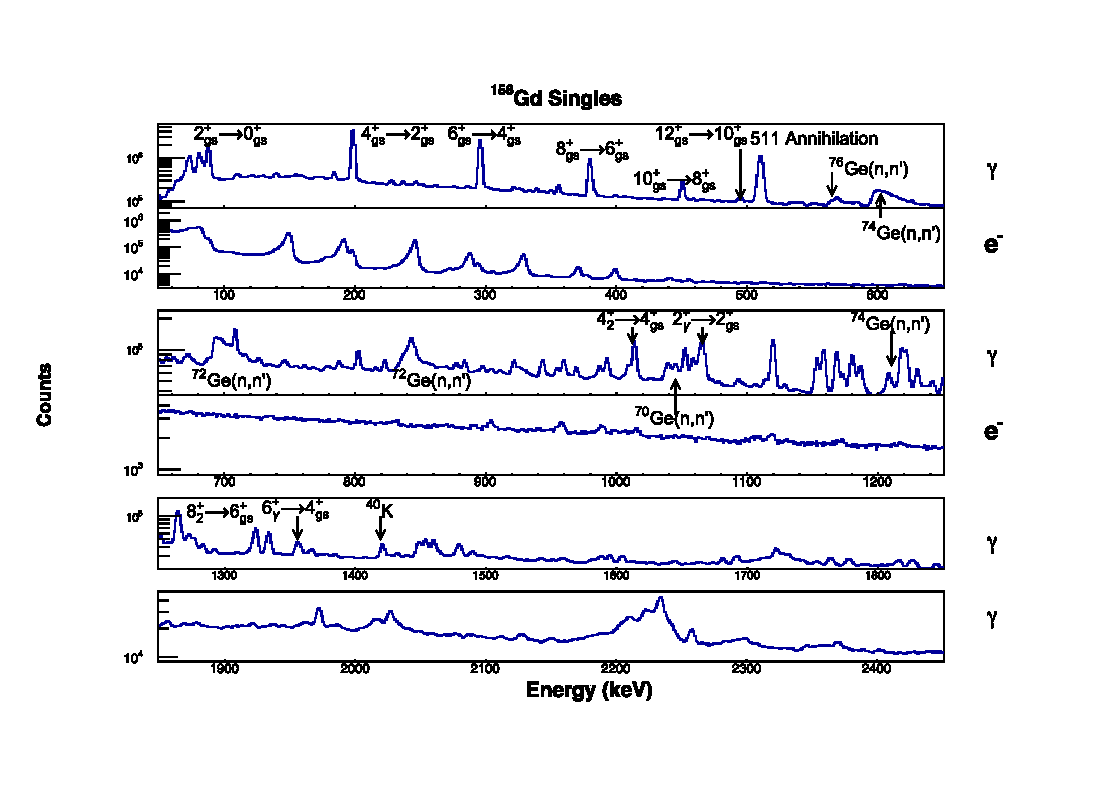
\includegraphics[scale=0.9]{156GdTablesAndFigs/156Gd_Singles_Label.eps}
    \caption{Singles spectra of $^{156}$Gd. Spectra are labeled with the particles being detected, the energies of the $\gamma$ and electron spectra aligned for identification. In the $\gamma$ spectrum, several lines of note are labeled. These are the ground-state band lines as well as other transitions of interest. Below 100 keV is a combination of x-rays and the 89 keV gamma from the ground state band. In the conversion electron spectrum, the large peaks up to approximately 350 keV are from the ground state band. These large peaks make the ground state band a good diagnostic, but also emphasize the need for coincidence gating, as the conversion electron spectrum is flooded by the ground state band electrons. The large peak at low energy is cut off due to the threshold. It is a combination of background and the 89L peak. Transitions in the higher energy regime of the $\gamma$ spectrum cannot be determined without gating, due to additional background from the experimental room.}
    \label{fig:156_Singles}
\end{figure}

As in the previous chapter, these transitions in the ground state are the first lines looked at in the data. These are all pure E2 multipole transitions, making them a diagnostic on the data compared with the theoretical coefficients from BrIcc\citep{kibedi08:_BRICC}. The transitions from $2^+$ to $10^+$ are summarized and compared with theory in Table \ref{tab:156Gd_Single_ICC_GS}.

\begin{landscape}
\footnotesize
    \begin{longtable}{c|c|c|c|c|c|c|c|c|c}
    \caption{$^{156}$Gd Ground State Band Internal Conversion Coefficients from Singles}
        \label{tab:156Gd_Single_ICC_GS}\\
    \toprule
$E$ (keV)	&	$J^{\pi}	\rightarrow	J^{\pi}$	&	$E_i$ (keV)	&	$E_f$ (keV)	&	$T_{1/2}$ (fs)	&	Multipolarity	&	Shell & $\alpha$ (This Work)	&	$\alpha$  (Th)	&	$\alpha$ (Konijn)	\\
\hline		
\endfirsthead
    \caption[]{$^{156}$Gd Ground State Band Internal Conversion Coefficients from Singles}\\
    \toprule
$E$ (keV)	&	$J^{\pi}	\rightarrow	J^{\pi}$	&	$E_i$ (keV)	&	$E_f$ (keV)	&	$T_{1/2}$ (fs)	&	Multipolarity	&	Shell & $\alpha$ (This Work)	&	$\alpha$  (Th)	&	$\alpha$ (Konijn)	\\
\hline		
\endhead
\endfoot
\multicolumn{10}{p{1.4\textwidth}}{A list of the ground state conversion coefficients from $^{156}$Gd. Multipolarities and mixing ratios were taken from NNDC. Unless otherwise stated, the $\alpha$ values are $\alpha_K$. An angular distribution correction has been applied based on multipolarities for pure transitions, and those with known mixing ratios. The first error is statistical, the second is systematic. Numbers are compared with Konijn et al. \citep{konijn81:_156gd} Starred values in the Konijn data were used as calibration points.}
\endlastfoot
198.58	&	$4^+	\rightarrow	2^+$	&	288.187	&	88.97	&	111900	&	E2	& K &	0.1667 (4)$^{+46}_{-45}$	&	0.1565 (22)	&	0.199 (36)	\\
	&				&		&		&		&		& L &	0.0537 (1)$^{+16}_{-15}$	&	0.0531 (8)	&		\\
	&			&		&		&		&		& M &	0.0170 (1) (5)	&	0.0122 (2)	&		\\ \hline
296.04	&	$6^+	\rightarrow	4^+$	&	584.715	&	288.187	&	15800	&	E2 & K	&	0.0572 (1) (18)	&	0.0477 (7)	&	0.04683*	\\
	&				&		&		&		&	& L	&	0.0121 (1) (4)	&	0.0115 (2)	&		\\
	&				&		&		&		&	& M	&	0.0036 (1) (1) &	0.0026 (1)	&		\\ \hline
379.92	&	$8^+	\rightarrow	6^+$	&	965.134	&	584.715	&	4320	&	E2 & K	&		0.0274 (1) (9)	&	0.0235 (4)	&	0.038 (10)	\\
	&				&		&		&		&	& L	&	0.0050 (1) (2)	&	0.0048 (1)	&		\\
	&				&		&		&		&	& M	&	0.0013 (1) (1)	&	0.0011 (1)	&		\\ \hline
450.64	&	$10^+	\rightarrow	8^+$	&	1416.078	&	965.134	&	1900	&	E2	& K &	0.0152 (2) (5)	&	0.01483 (21)	& 0.0145*		\\
	&				&		&		&		&	& L	&	0.0028 (1) (1)	&	0.00279 (4)	&		\\
	&				&		&		&		&	& M	&	0.0010 (1) (1)	&	0.000621 (9)	&		\\ 
\bottomrule
    \end{longtable}
\end{landscape}

Unlike the $^{154}$Gd data, there did not appear to be contaminants in these ground state lines, outside of the $2^+\rightarrow0^+$ transition. This transition was also considered unreliable, as the low energy of the $\gamma$-ray put it before the efficiency turnover. The change in efficiency in the HPGe detectors is steep in this region, leading to large uncertainty.

\section{Gates on the Ground State Band}

The transitions of the ground state band were the most prominent peaks in the spectra (Figure \ref{fig:156_Singles}). The high number of counts in these peaks made them prime candidates to gate on and build up a level scheme. Only the $\gamma$ components were gated on, as the electron components wide width made it difficult to gate on the whole of the peak without contaminants. Figures \ref{fig:156_2to0}, \ref{fig:156_4to2}, \ref{fig:156_6to4}, and \ref{fig:156_8to6} are the result of these gates. Unlike the gates in $^{154}$Gd, the $4^+\rightarrow2^+$ gate was the most fruitful, due to the challenges of the $2^+\rightarrow0^+$ transition posed. 

\afterpage{\clearpage\begin{figure}[!]
    \centering
    \begin{subfigure}{\textwidth}
    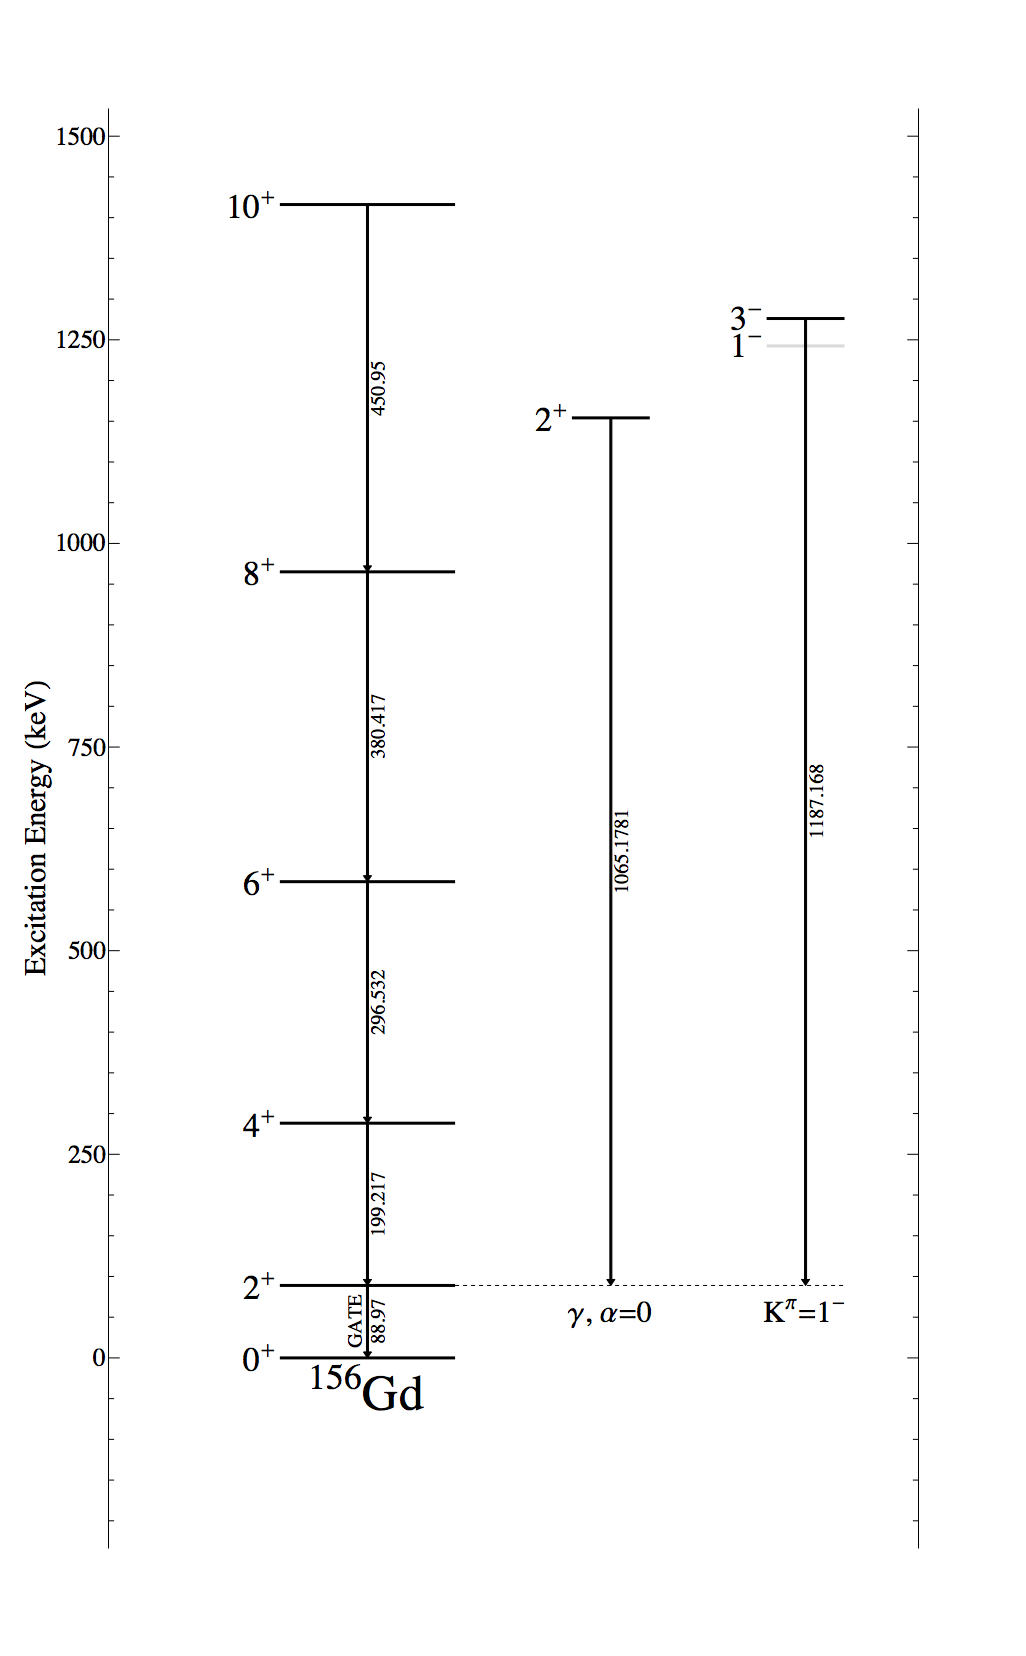
\includegraphics[scale=0.4]{156GdTablesAndFigs/156Gd_2to0.eps}
    \caption{\label{fig:156_2to0level}Level Scheme of $^{156}$Gd. The gamma ray of the $2^+$\rightarrow$0^+$ (89 keV) transition in the ground state was gated on. It was then compared with the gated spectrum from the gamma ray of the $4^+$\rightarrow$2^+$ (199 keV) transition in the ground state. Peaks only appearing in the first gate were assumed to go into the $2^+$ state, and assignments were made. Due to the low energy of the $2^+$\rightarrow$0^+$ transition, the efficiency was lower, and it is likely that transitions into the $2^+$ state were missed. The levels are organized by band. The lower levels of the band, unseen by gamma rays in this gate, are in gray.}
    \end{subfigure}
    \captionlistentry{Level scheme and spectrum of $^{156}$Gd based on the $2^+\rightarrow0^+$ transition.}
    \label{fig:156_2to0}
    \end{figure}
\begin{landscape}
    \begin{figure}
    \ContinuedFloat
    \begin{subfigure}{1.4\textwidth}
    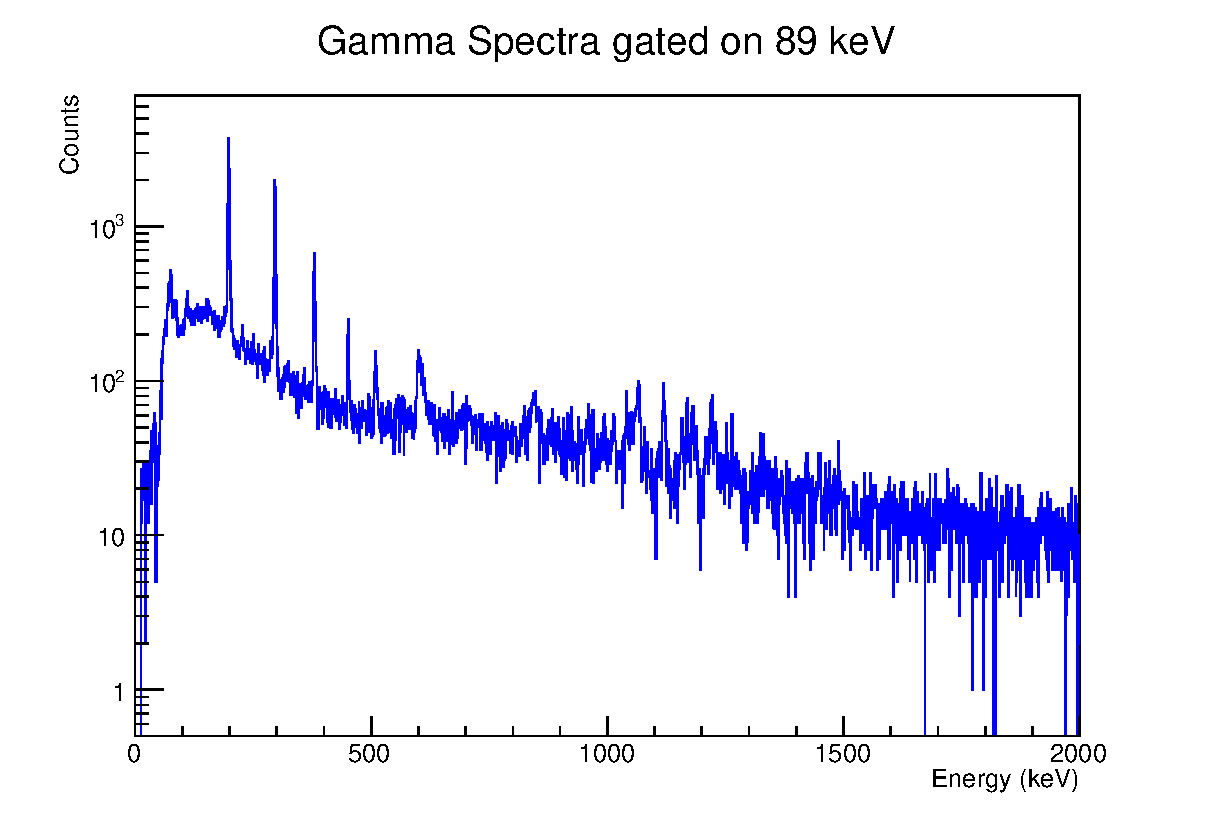
\includegraphics[]{156GdTablesAndFigs/89GateSpectrum.eps}
    \caption{Gamma spectrum gated on 89 keV, corresponding to the $2^+\rightarrow0^+$ transition.}
    \label{fig:156_2to0spec}
    \end{subfigure}
\end{figure}
\end{landscape}}

\afterpage{\clearpage\begin{landscape}
\begin{figure}
    \centering
    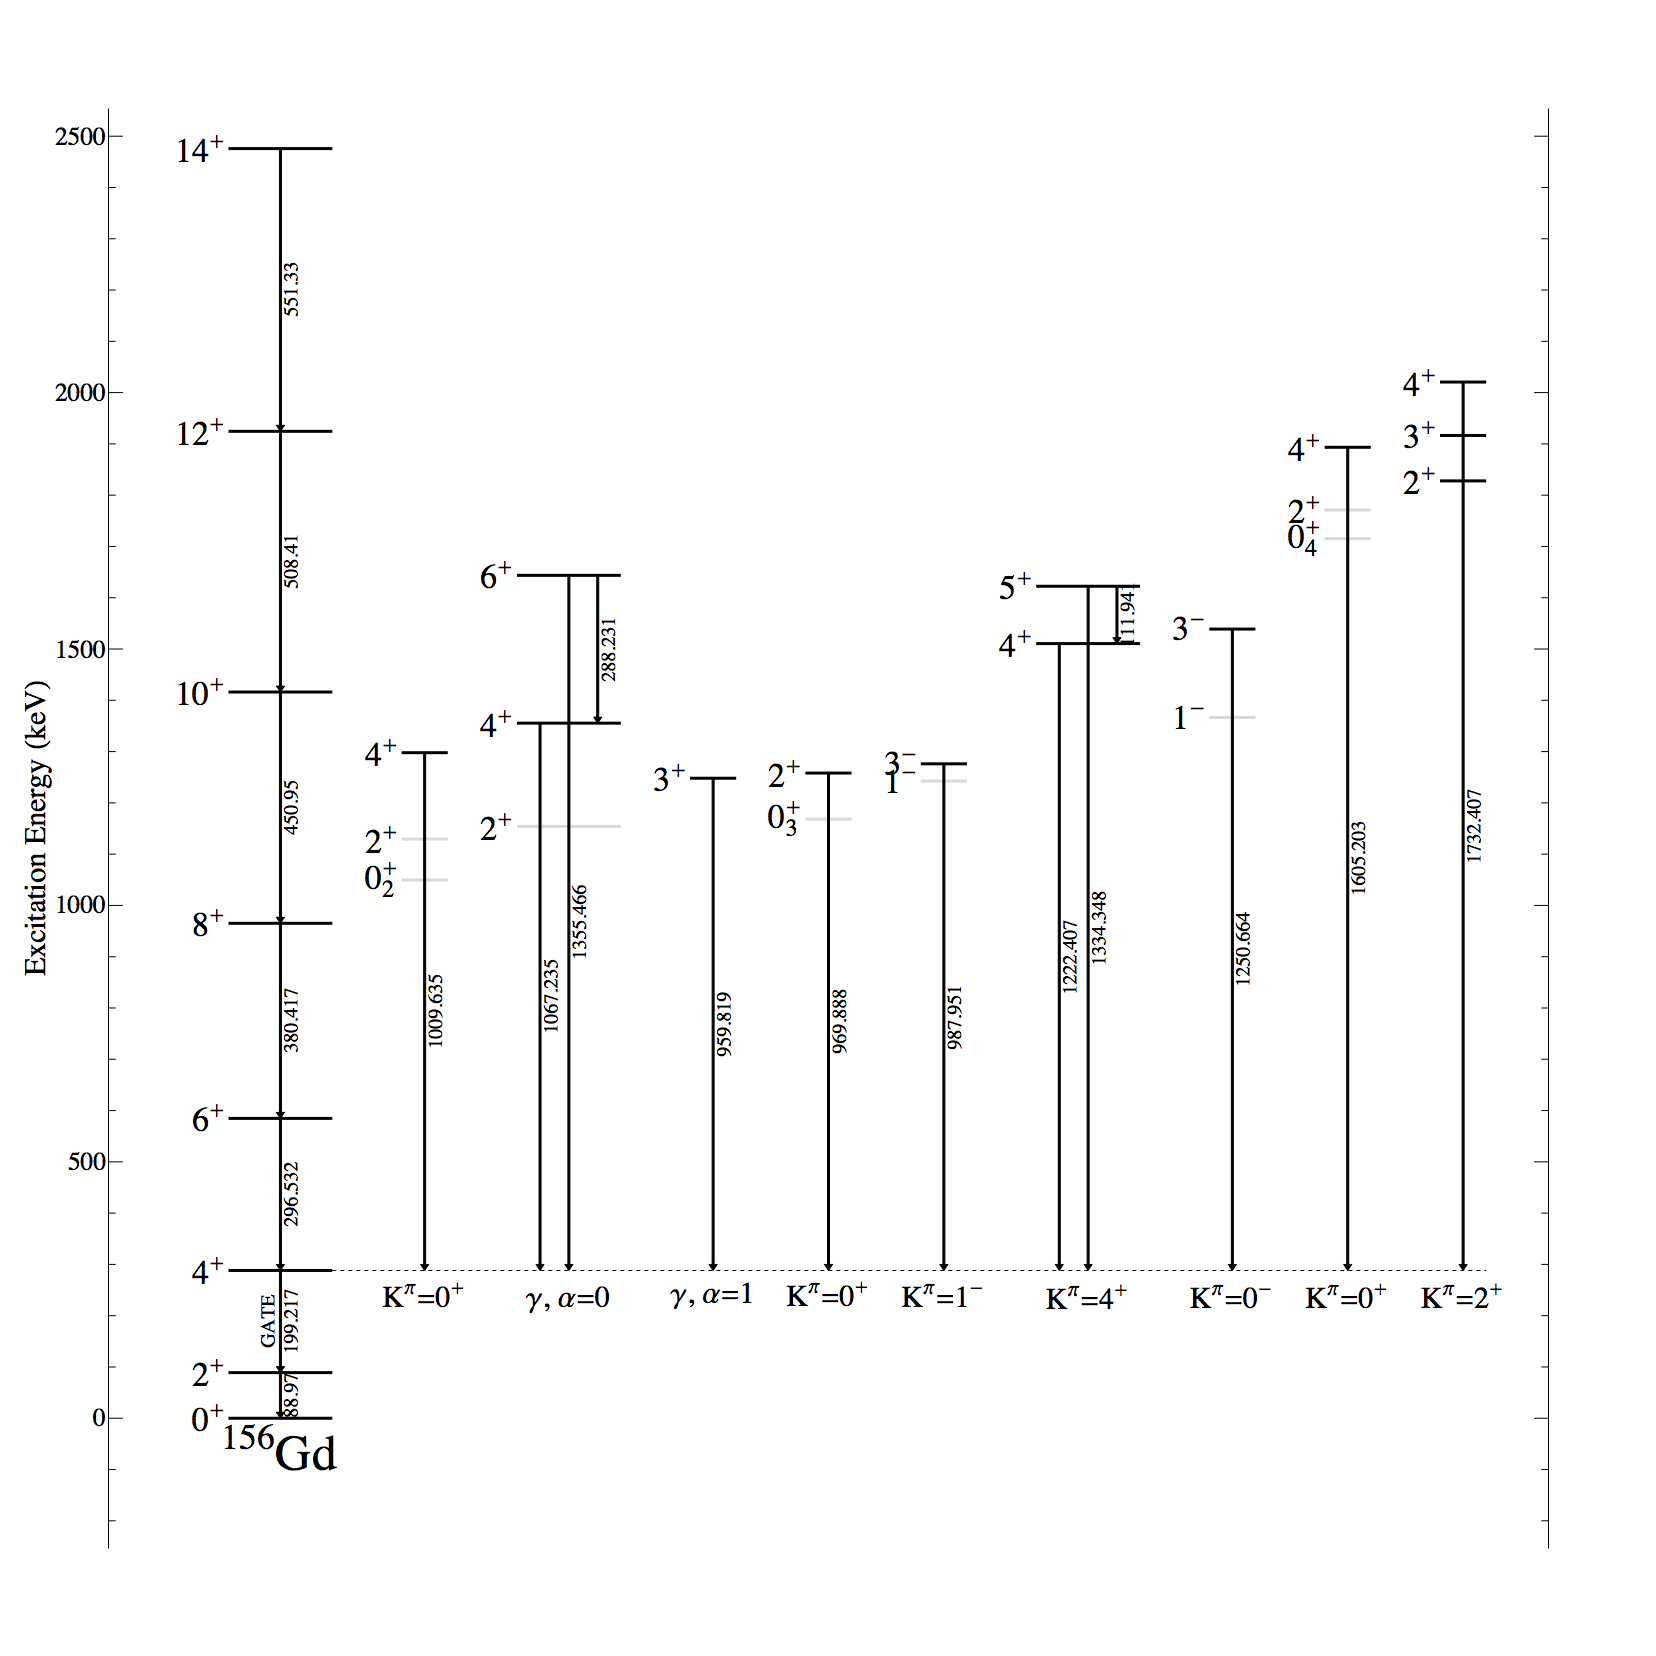
\includegraphics[scale=0.4]{156GdTablesAndFigs/156Gd_4to2.eps}
    \caption{Level Scheme of $^{156}$Gd. The gamma ray of the $4^+$\rightarrow$2^+$ (199 keV) transition in the ground state was gated on. It was then compared with the gated spectrum from the gamma ray of the $6^+$\rightarrow$4^+$ (296 keV) transition in the ground state. Peaks only appearing in the first gate were assumed to go into the $4^+$ state, and assignments were made. Additionally, these peaks were also gated on, to look for cascades leading into the $4^+$ state, which were found in several cases. The levels are organized by band. The lower levels of the band, unseen by gamma rays in this gate, are in gray.}
    \label{fig:156_4to2}
\end{figure}
\end{landscape}}

\afterpage{\clearpage\begin{figure}
    \centering
    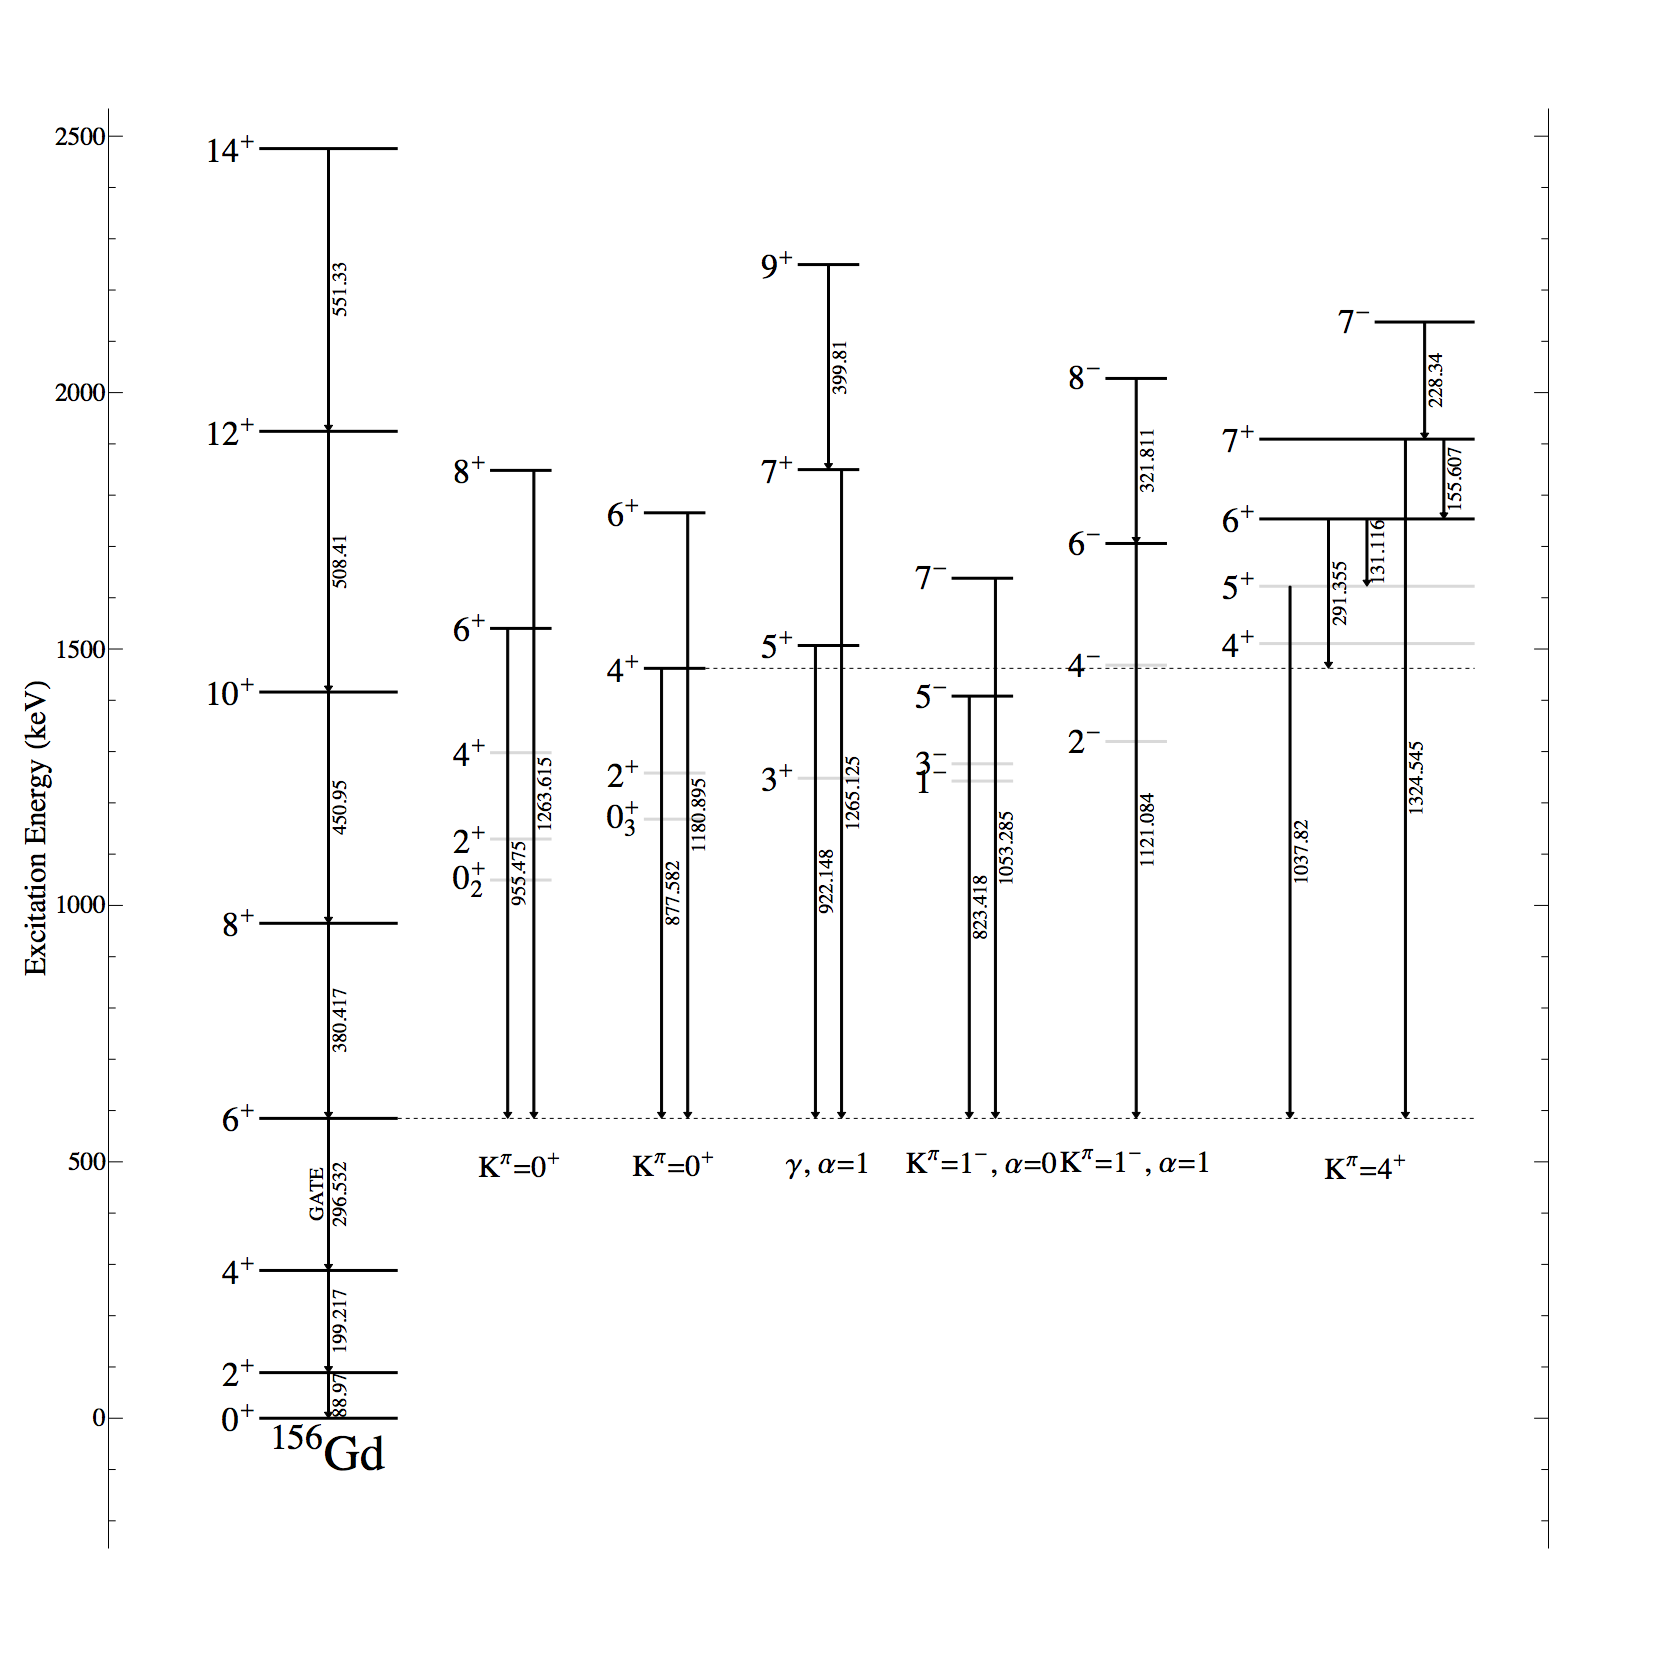
\includegraphics[scale=0.28]{156GdTablesAndFigs/156Gd_6to4.png}
    \caption{Level Scheme of $^{156}$Gd. The gamma ray of the $6^+$\rightarrow$4^+$ (296 keV) transition in the ground state was gated on. It was then compared with the gated spectrum from the gamma ray of the $8^+$\rightarrow$6^+$ (380 keV) transition in the ground state. Peaks only appearing in the first gate were assumed to go into the $6^+$ state, and assignments were made. Additionally, these peaks were also gated on, to look for cascades leading into the $6^+$ state, which were found in several cases. The levels are organized by band. The lower levels of the band, unseen by gamma rays in this gate, are in gray.}
    \label{fig:156_6to4}
\end{figure}}

\afterpage{\clearpage\begin{figure}
    \centering
    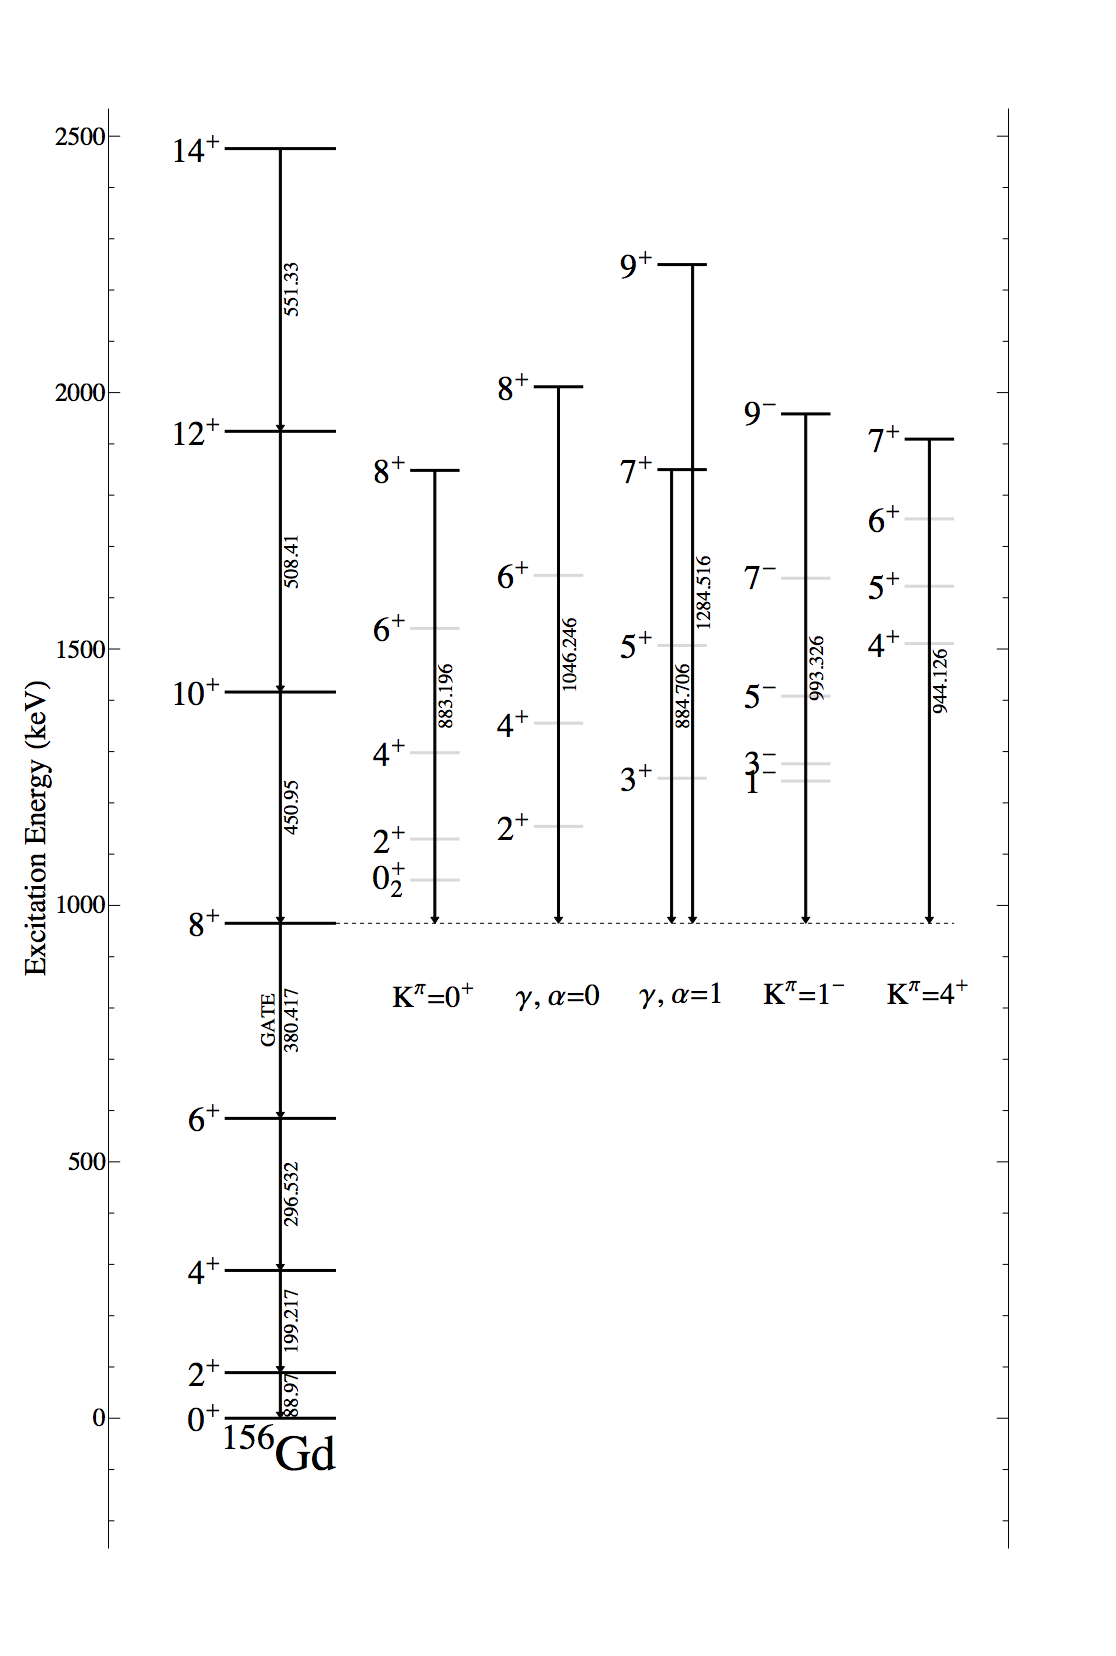
\includegraphics[scale=0.3]{156GdTablesAndFigs/156Gd_8to6.png}
    \caption{Level Scheme of $^{156}$Gd. The gamma ray of the $8^+$\rightarrow$6^+$ (380 keV) transition in the ground state was gated on. It was then compared with the gated spectrum from the gamma ray of the $10^+$\rightarrow$8^+$ (451 keV) transition in the ground state. Peaks only appearing in the first gate were assumed to go into the $8^+$ state, and assignments were made. Additionally, these peaks were also gated on, to look for cascades leading into the $8^+$ state, which were found in several cases. The levels are organized by band. The lower levels of the band, unseen by gamma rays in this gate, are in gray.}
    \label{fig:156_8to6}
\end{figure}}

Determining which transitions went uniquely into a given ground state level was done by comparing the outgoing ground state transition for that level with the incoming transitions, i.e. the $4^+\rightarrow2^+$ (199 keV) gate was compared directions with the $6^+\rightarrow4^+$ (296 keV) gate. The $\gamma$-spectra corresponding to these lines can be seen in Figure \ref{fig:156_GS_Gate}. Lines in the gamma spectrum that were present only in the outgoing spectrum, but not the incoming spectrum, are going into that level (the $4^+$ in the example above). Identified transitions were then gated on to confirm assignments and search for cascades from higher energy states.

\begin{figure}[!]
    \centering
    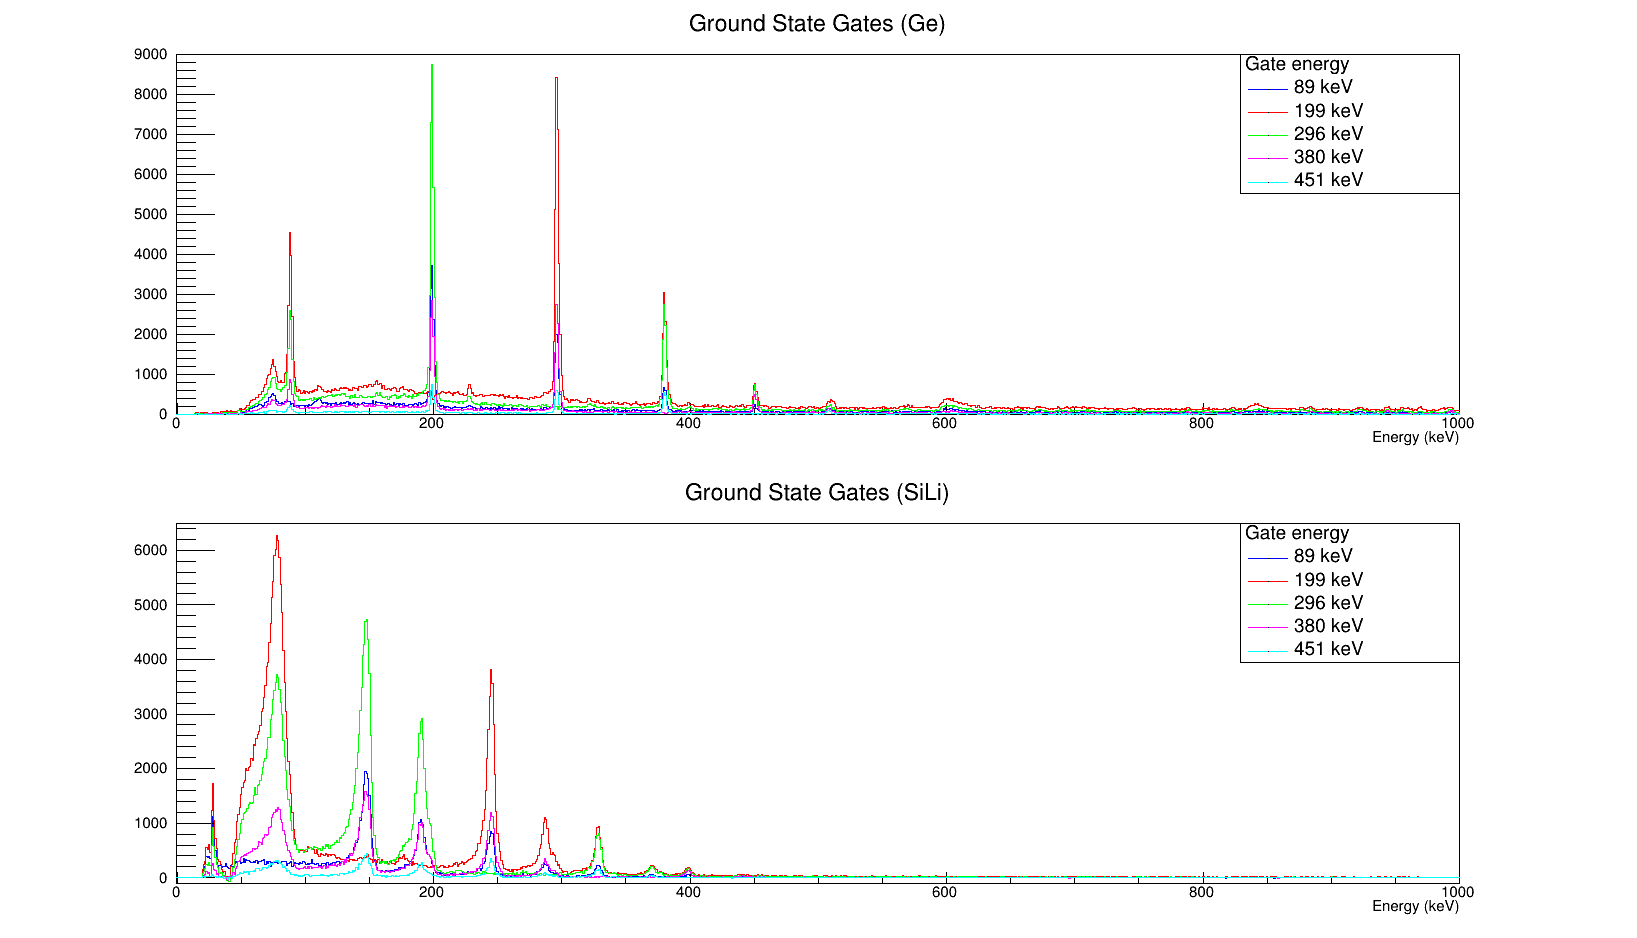
\includegraphics[scale=0.27]{156GdTablesAndFigs/156GS_stack.png}
    \caption{Spectra gated on the ground state band lines of $^{156}$Gd. As can be seen, some lines do not appear in different gates. Comparison of these gates, for instance 199 keV ($4^+\rightarrow2^+$) and 296 keV ($6^+\rightarrow4^+$), yields a list of transitions that directly populate the interim level (in the example, the $4^+$ state). The 89 keV line, although the lowest transition in the ground state band, has a low yield due to efficiency, and is reflected in the relative size of the peaks. The 199 keV peak in the gamma spectrum is much larger from the 296 keV transition than the 89 keV transition.}
    \label{fig:156_GS_Gate}
\end{figure}

In this data, the secondary gate check was especially important, as the low efficiency of the $2^+\rightarrow0^+$ transition would have meant weaker lines going into the $2^+$ state could be falsely assigned going into the $4^+$ state. As the ground state band transitions are so prolific, the transitions showed up when gating on weaker peaks in the spectra, while the inverse was not always true.

Little could be seen in the $2^+\rightarrow0^+$ gate, as it reflected in Figure \ref{fig:156_2to0}. The $4^+\rightarrow2^+$ gate shows far more, seen in Figure \ref{fig:156_4to2}, including evidence of populating 3 excited $0^+$ bands. In total, nine bands were seen in the gating outside of the ground state band. The number of bands seen drops off with higher gates, both due to the drop off in populating higher energy states and the drop off in populating higher $J$ states. Also seen in the gates are the $\gamma$-vibrational band, the $K=1^-$ octopole band, and a $K=4^+$ band.

\section{Conversion Coefficients from Singles}

With the gamma-rays now identified through gates, conversion coefficients could be calculated from singles spectra. Tables \ref{tab:156Gd_Single_ICC_Corr}, \ref{tab:156Gd_Single_ICC_Uncorr}, and \ref{tab:156Gd_No_Mult_ICC} are these results. Where available, results were compared with Konijn et al\citep{konijn81:_156gd}. Results are compared against this data, as it also examined the nucleus via an $(\alpha,2n)$ reaction.

Transitions that could be clearly identified and separated are found in Table \ref{tab:156Gd_Single_ICC_Corr}. Contamination concerns were taken into account by using the identified transitions to look for gamma-rays in close proximity to those in the Table. These transitions all have known multipole assignments and mixing ratios as needed, allowing for angular corrections. Two transitions with possible $E0$ components are seen in this Table. One, the $2^+\rightarrow2^+$ transition, appears to has a clear E0 component. Although this transition was not used in Figure \ref{fig:156_2to0}, the band the state exists in is populated, as seen in figures \ref{fig:156_4to2}, \ref{fig:156_6to4}, and \ref{fig:156_8to6}. The $6^+\rightarrow6^+$ transition does not appear to have an $E0$ component. While the value agrees with Konijn\citep{konijn81:_156gd}, it does not agree with the theoretical value for an $E2$, the multipole the transition has been assigned.

\afterpage{\clearpage\begin{landscape}
    \begin{longtable}{>{\footnotesize}c|>{\footnotesize}c|>{\footnotesize}c|>{\footnotesize}c|>{\footnotesize}c|>{\footnotesize}c|>{\footnotesize}c|>{\footnotesize}c|>{\footnotesize}c|>{\footnotesize}c|>{\footnotesize}c}
    \caption{$^{156}$Gd Internal Conversion Coefficients from Singles}
        \label{tab:156Gd_Single_ICC_Corr}\\
    \toprule
$E$ (keV)	&	$J^{\pi}	\rightarrow	J^{\pi}$	&	$E_i$ (keV)	&	$E_f$ (keV)	&	$T_{1/2}$ (fs)	&	Multipolarity	&	$\delta$	& Shell &	$\alpha$ (This Work)	&	$\alpha$  (Theory)\citep{kibedi08:_BRICC}	&	$\alpha$ (Konijn)\citep{konijn81:_156gd}	\\
\hline		
\endfirsthead
    \caption[]{$^{156}$Gd Internal Conversion Coefficients from Singles}\\
    \toprule
$E$ (keV)	&	$J^{\pi}	\rightarrow	J^{\pi}$	&	$E_i$ (keV)	&	$E_f$ (keV)	&	$T_{1/2}$ (fs)	&	Multipolarity	&	$\delta$ & Shell &	$\alpha$ (This Work)	&	$\alpha$  (Theory)\citep{kibedi08:_BRICC}	&	$\alpha$ (Konijn)\citep{konijn81:_156gd}	\\
\hline		
\endhead
\endfoot
\multicolumn{11}{p{1.4\textwidth}}{A list of conversion coefficients from $^{156}$Gd. Multipolarities and mixing ratios were taken from the nuclear date sheets\citep{reich12:_nds_156}. Unless otherwise stated, the $\alpha$ values are $\alpha_K$. An angular distribution correction has been applied based on multipolarities for pure transitions, and those with known mixing ratios. The first error is statistical, the second is systematic. Numbers are compared with Konijn et al\citep{konijn81:_156gd}.}
\endlastfoot
227.90	&	$7^-_{7^-}	\rightarrow 7^+_{4^+}$	&	2137.6	&	1909.26	&	1300000000	&	E1	&	& K	&	0.4687 (50)$^{+85}_{-84}$	&	0.0272 (4)	&	0.063 (13)	\\
	&			&		&		&		&		&	& LM	&	0.1073 (20) (20)	&	0.0049 (6)	&		\\ \hline
321.92	&	$8^-_{1^-}	\rightarrow	6^-_{1^-}$	&	2027.1	&	1705.799	&		&	E2	&		& K &	0.0290 (13) (9)	&	0.0378 (6)	&	0.025 (7)	\\ \hline
355.87	&	$4^+_{4^+}	\rightarrow	2^+_{\gamma}$	&	1510.594	&	1154.152	&	189000	&	E2	&		& K &	0.0158 (6) (5)	&	0.0281 (4)	&	\\ \hline
399.56	&	$9^+_{\gamma}	\rightarrow	7^+_{\gamma}$	&	2249.65	&	1849.84	&		&	E2	&		& K &	0.0077 (8) (3)	&	0.0205 (3)	&	0.026 (5)	\\ \hline
921.83	&	$5^+_{\gamma}	\rightarrow	6^+_{gs}$	&	1506.863	&	584.715	&	400	&	E2	&		& K &	0.0041 (9) (5) &	0.0028 (1)	&	0.0030 (7)	\\ \hline
1040.470	&	$2^+_{0^+_{2}}	\rightarrow	2^+_{gs}$	&	1129.437	&	88.970	&		&	E2+E0+M1	&	$-5.9^{+14}_{-28}$	& K &	0.0152 (10) (2)	&	0.0022 (1)	&	0.014 (3)	\\ \hline
1059.31	&	$6^+_{\gamma}	\rightarrow	6^+_{gs}$	&	1643.653	&	584.715	&		&	E2	&		& K &	0.0013 (5) (1)	&	0.0021 (1)	&	0.0013 (8)	\\ \bottomrule
    \end{longtable}
\end{landscape}}

Table \ref{tab:156Gd_Single_ICC_Uncorr} holds conversion coefficients that have been left uncorrected in the singles for one of two reaons: either there were multiple known assignments to the gamma-ray energy, or the exact multipole mixing-ratio $\delta$ was unknown. Several of these transitions are high energy $J^\pi\rightarrow J^\pi$ transitions if the assignment is correct without extra contamination. This includes a $0^+\rightarrow0^+$ transition. The Si(Li) efficiency at these energies was too low to see the conversion electrons in gated spectra.

\afterpage{\clearpage	\begin{ThreePartTable}
		\begin{longtable}{>{\footnotesize}c|>{\footnotesize}c|>{\footnotesize}c|>{\footnotesize}c|>{\footnotesize}c|>{\footnotesize}c|>{\footnotesize}c}
			\caption{Uncorrected $^{156}$Gd Internal Conversion Coefficients from Singles\label{tab:156Gd_Single_ICC_Uncorr} }\\
			\multicolumn{6}{c}{(a)} \\
			\toprule
	& & & & & \\
	$E$ (keV)	&	$J^{\pi}	\rightarrow	J^{\pi}$	&	$E_i$ (keV)	&	$E_f$ (keV)	& $T_{1/2}$ (fs) &	Multipolarity	&	$\delta$ \\
	\hline
	\endfirsthead
	\caption[]{Uncorrected $^{156}$Gd Internal Conversion Coefficients from Singles} \\
	\multicolumn{6}{c}{(a)} \\
	\toprule
	$E$ (keV)	&	$J^{\pi}	\rightarrow	J^{\pi}$	&	$E_i$ (keV)	&	$E_f$ (keV)	& $T_{1/2}$ (fs) &	Multipolarity	&	$\delta$ \\
	\hline
	\endhead
154.94	&	$4^+_{4^+}	\rightarrow	4^+_{\gamma}$	&	1510.594	&	1355.422	&	189000	&	M1+E2	&	0.48	\\
	&	$7^+_{4^+}	\rightarrow	6^+_{4^+}$	&	1909.26	&	1753.653	&		&	(M1+E2)	&	0.29	\\ \hline
883.86	&	$8^+_{0^+_{2}}	\rightarrow	8^+_{gs}$	&	1848.33	&	965.134	&		&	E0+E2	&		\\
	&	$7^+_{\gamma}	\rightarrow	8^+_{gs}$	&	1849.84	&	965.134	&		&	E2(+M1)	&		\\ 
	&		&		&	&		&	\\ \hline
955	&	$6^+_{0^+_{2}}	\rightarrow	6^+_{gs}$	&	1540.19	&	584.715	&		&	E0+E2	&		\\ 
959.88	&	$0^+_{0^+_{2}}	\rightarrow	2^+_{gs}$	&	1049.487	&	88.97	&	1800	&	E2	&			\\
	&	$3^+_{\gamma}	\rightarrow	4^+_{gs}$	&	1248.006	&	288.197	&	580	&	E2+M1	&	-12	\\ \hline
1009.33	&	$4^+_{0^+_{2}}	\rightarrow	4^+_{gs}$	&	1297.822	&	288.197	&	1600	&	E0+E2,M1	&		\\ 
&		&		&	&		&	\\ \hline
1045.48	&	$8^+_{\gamma}	\rightarrow	8^+_{gs}$	&	2011.38	&	965.134	&		&	E2(+M1)	&		\\ 
&		&		&	&		&	\\ 
1052.61	&	$7^-_{1^-}	\rightarrow	6^+_{gs}$	&	1638	&	584.715	&		&	E1	&		\\ \hline
1065.74	&	$2^+_{\gamma}	\rightarrow	2^+_{gs}$	&	1154.152	&	88.97	&	568	&	E2+M1	&	-16	\\
	&	$4^+_{\gamma}	\rightarrow	4^+_{gs}$	&	1355.422	&	288.187	&	540	&	E2+M1	&	-4	\\ \hline
1158.65	&	$2^+_{\gamma}	\rightarrow	0^+_{gs}$	&	1154.152	&	0	&	568	&	E2	&		\\
	&	$3^+_{\gamma}	\rightarrow	2^+_{gs}$	&	1248.006	&	88.97	&	580	&	E2+M1	&	-11.8	\\ \hline
1168.69	&	$0^+_{0^+_{3}}	\rightarrow	0^+_{gs}$	&	1168.186	&	0	&	5000	&	E0	&		\\
	&	$2^+_{0^+_{3}}	\rightarrow	2^+_{gs}$	&	1258.075	&	88.97	&	1540	&	E2+M1+E0	&	0.38	\\ \hline
1222.22	&	$4^+_{4^+}	\rightarrow	4^+_{gs}$	&	1510.594	&	288.197	&	189000	&	M1+E2	&	-1.7	\\
	&	$5^+_{\gamma}	\rightarrow	4^+_{gs}$	&	1506.863	&	288.197	&	400	&	E2	&		\\ \hline
1264.85	&	$4^+_{\gamma}	\rightarrow	2^+_{gs}$	&	1355.422	&	88.97	&	540	&	E2	&		\\
	&	$8^+_2	\rightarrow	6^+_{gs}$	&	1848.33	&	584.715	&		&		\\
	&	$7^+_{\gamma}	\rightarrow	6^+_{gs}$	&	1849.84	&	584.715	&		&		\\ 
	&		&		&	&		&	\\ 
	\bottomrule
\end{longtable}
\end{ThreePartTable}
\pagebreak
\begin{ThreePartTable}
	\begin{TableNotes}[para]
		Table \ref{tab:156Gd_Single_ICC_Uncorr}: A list of conversion coefficients from $^{156}$Gd. Multipolarities and mixing ratios were taken from the nuclear data sheets\citep{reich12:_nds_156}. Unless otherwise stated, the $\alpha$ values are $\alpha_K$. No angular distribution correction has been applied, either due to unknown mixing ratios, or multiple assignments of the gamma-ray. The first error is statistical, the second is systematic. Numbers are compared with Konijn et al. \citep{konijn81:_156gd} Starred values were used as calibration points in the Konijn paper. All coefficients are K-shell electrons.
	 \end{TableNotes}
\begin{longtable*}{>{\footnotesize}c|>{\footnotesize}c|>{\footnotesize}c|>{\footnotesize}c|>{\footnotesize}c|>{\footnotesize}c}
	%\multicolumn{6}{c}{\MakeUppercase{Table \ref{tab:156Gd_Single_ICC_Uncorr} (Continued)}} \\
	\multicolumn{6}{c}{\MakeUppercase{Table 5.4 (Continued)}} \\
	\multicolumn{6}{c}{(b)} \\
	\toprule
	&  & \multicolumn{2}{>{\footnotesize}c|}{$\alpha$ (This Work)} & & \\
	$E$ (keV)	& Shell	&	Uncorrected & Corrected &	$\alpha$  (Th)\citep{kibedi08:_BRICC}	&	$\alpha$ (Konijn)\citep{konijn81:_156gd} \\
	\hline
	\endfirsthead
	%\multicolumn{6}{c}{\MakeUppercase{Table \ref{tab:156Gd_Single_ICC_Uncorr} (Continued)}} \\
	\multicolumn{6}{c}{\MakeUppercase{Table 5.4 (Continued)}} \\
	\multicolumn{6}{c}{(b)} \\
	\toprule
	&  & \multicolumn{2}{>{\footnotesize}c|}{$\alpha$ (This Work)} & & \\
	$E$ (keV)	& Shell	&	Uncorrected & Corrected &	$\alpha$  (Th)\citep{kibedi08:_BRICC}	&	$\alpha$ (Konijn)\citep{konijn81:_156gd} \\
	\hline
	\endhead
	154.94	& K & 	0.4635 (183)$^{+98}_{-97}$	& 0.3462 (137)$^{+73}_{-72}$ &	0.460 (7)	& \\
	&		 K &	0.4879 (193)$^{+103}_{-102}$ &	0.474 (7)	&		\\ \hline
883.86	& K &	0.0057 (7) (1)	& 0.0034 (4) (1) &	0.0030 (1)	& $>0.0092$		\\
& K &		&	[M1] 0.0102 (13) (2) & [M1] 0.0052 (1)	&	$<0.0052$	\\ 
&  &		&	[E2] 0.0073 (9) (1) & [E2] 0.0030 (1)	&		\\ \hline
955	& K &	0.0065 (4) (5)	& 0.0039 (2) (3) &	0.0026 (1)	&	0.020 (8)	\\ 
959.88	& K & &	0.0136 (8) (10) &  0.0025 (1)	&	0.0045 (24)	\\
& K &		&	0.0120 (7) (9) & 0.0025 (1)	&		\\ \hline
1009.33	& K &	0.0173 (9) (4)	& [M1] 0.0234 (12) (5) &	[M1] 0.0038 (1)	&	0.0164 (29)	\\ 
&  &		&	[E2] 0.0107 (6) (2) & [E2] 0.0023 (1)	&		\\ \hline
1045.48	& K &	0.0012 (2) (2)	& [M1] 0.0015 (3) (3)	 & [M1] 0.0035 (1)	&	0.0025 (6)	\\ 
&  &		&	[E2] 0.0007 (1) (1) & [E2] 0.0021 (1)	&		\\ 
1052.61	& K & &  0.0008 (1) (1)	&	0.0009 (1)	&		\\ \hline
1065.74	& K &	0.0023 (2) (1)	& 0.0034 (3) (1) &	0.0021 (1)	&	0.0025 (9)	\\
& K &		&	0.0029 (3) (1) & 0.0021 (3)	&	0.0021 (1)	\\ \hline
1158.65	& K &	0.0020 (3) (1)	& 0.0020 (3) (1) &	0.0017 (1)	&	0.0023 (3)	\\
& K & & 0.0014 (2) (1)		&	0.0017 (1)	&		\\ \hline
1168.69	& K &	0.0045 (3) (1)	& 0.0045 (3) (1) & 		&	$>0.0035$	\\
& K &	& 0.0038 (3) (1)	&	0.0026 (1)	&		\\ \hline
1222.22	& K &	0.0028 (4) (1)	 & 0.0031 (4) (1) &	0.0018 (1)	&	0.00174*	\\
& K &		& 0.0031 (4) (1)	& 0.001560 (22)	&	\\ \hline
1264.85	& K &	0.0017 (3) (1) & 0.0014 (2) (1)	&	0.0014 (1)	&	\\
& K &		& [E2] 0.0014 (2) (1)	&	[E2] 0.0014 (1) &		\\
& K &		& [M1] 0.0011 (2) (1)	& [M1] 0.0022 (1)	&		\\ 
&		&		&	[E2] 0.020 (3) (1) & [E2] 0.0014 (1)	&		\\
	\bottomrule
	\insertTableNotes
\end{longtable*}

\end{ThreePartTable}}

Table \ref{tab:156Gd_No_Mult_ICC} has conversion coefficients that could not be corrected due to the transitions having unknown multipole assignments. Allowable and reasonable theoretical conversion coefficients from BrIcc\citep{kibedi08:_BRICC} are listed in the table.

\afterpage{\clearpage\begin{landscape}
    \begin{longtable}{c|c|c|c|c|c|c|c|c}
        \caption{$^{156}$Gd Internal Conversion Electrons without known Multipolarities}
        \label{tab:156Gd_No_Mult_ICC}\\
        \toprule
        &	& 	&  &	& \multicolumn{2}{c}{Theory}	& 	\\
        $E_i$ (keV)	&	$E_f$ (keV)	& $E$ (keV)	&	Gate &		$\alpha$ (This Work)	& $\alpha$(M1) & $\alpha$(E2) & $\alpha$(E1) &	$\alpha$ (Konijn)	\\
        \hline		
        \endfirsthead
        \caption[]{$^{156}$Gd Internal Conversion Electrons without known Multipolarities}\\
        \toprule
        &	& 	&  &	& \multicolumn{2}{c}{Theory}	& 	\\
        $E_i$ (keV)	&	$E_f$ (keV)	& $E$ (keV)	&	Gate &		$\alpha$ (This Work)	& $\alpha$(M1) & $\alpha$(E2) & $\alpha$(E1) &	$\alpha$ (Konijn)	\\
        \hline		
        \endhead
        671.41	&	$7^-	\rightarrow	8^+$	&	1638	&	965.134	&		0.0064 (6) (2)	& & & 0.00213 (3) &	\\ \hline
        838.83	&	$9^+	\rightarrow	10^+$	&	2249.65	&	1416.078	&	0.0009 (3) (1)	& 0.00595 (9) & 0.00337 (5) & & 	\\ \hline
        943.732	&	$7^+	\rightarrow	8^+$	&	1909.26	&	965.134		&	0.0022 (6) (1) & 0.00448 (7) & 0.00262 (4) & &	0.0025 (3)	\\ 
        \bottomrule
    \end{longtable}
    \caption{A list of conversion coefficients from $^{156}$Gd without known multipolarities. As a result, an angular distribution correction term has not been applied. None of the states have known half lives. The first error is statistical, the second is systematic. Numbers are compared with theoretical values for allowed multipolarities and results from Konijn et al. \citep{konjin81:_156gd}. All coefficients are K-shell electrons.}
\end{landscape}}

\section{$J^{\pi}\rightarrow J^{\pi}$ Transitions}

After identification of the bands and transitions, gates were put on the transitions both entering and leaving states of interest, namely even-$J^+$ states. Gates entering these states (incoming transitions) were not fruitful. This is unfortunate for the $0^+$ states, as only incoming transitions can be used for transitions to the ground state. Gates leaving the states (outgoing transitions), had more statistics, and results could be obtained. $J^\pi\rightarrow J^\pi$ transitions up to $4^+$ were seen. Tables \ref{tab:156Gd_0_to_0}, \ref{tab:156Gd_2_to_2}, and \ref{tab:156Gd_4_to_4} are the tabulated results. These values are compared with Konijn\citep{konijn81:_156gd} where available. Additionally, the theoretical conversion coefficients have been listed for the $M1$ and $E2$ transitions, as taken from BrIcc\citep{kibedi08:_BRICC}.

In Table \ref{tab:156Gd_0_to_0}, only one $0^+\rightarrow0^+$ transition could be seen with enough statistics to get a value. All other possible $0^+\rightarrow0^+$ transitions were at high energies with such low efficiency in the Si(Li) detectors that a peak could not be seen.
    
\afterpage{\clearpage\begin{landscape}
    \begin{longtable}{c|c|c|c|c|c|c|c|c}
        \caption{$0^+\rightarrow 0^+$ Transitions in $^{156}$Gd}
        \label{tab:156Gd_0_to_0}\\
        \toprule
        &	& & & 	&  &	& \multicolumn{2}{c}{Theory}	\\
        $E_i$ (keV)	& Band &	$E_f$ (keV)	& Band &$E$ (keV)	&	Gate &		$\alpha$ (This Work)	& $\alpha$(M1) & $\alpha$(E2) \\
        \hline
        \endfirsthead
        \toprule
        \caption[]{$0^+\rightarrow 0^+$ Transitions in $^{156}$Gd}\\
        & & &	& 	&  &	& \multicolumn{2}{c}{Theory}	\\
        $E_i$ (keV)	& Band &	$E_f$ (keV)	& Band &$E$ (keV)	&	Gate &		$\alpha$ (This Work)	& $\alpha$(M1) & $\alpha$(E2) \\
	    \endhead
	    \endfoot
	    \multicolumn{9}{p{1.4\textwidth}}{A list of conversion coefficients from $^{156}$Gd for $0^+\rightarrow 0^+$ transitions seen in the gated data. All listed theoretical values are for the K-shell internal conversion coefficient. Numbers are compared with theoretical values for illustration. All coefficients are K-shell electrons. }
	    \endlastfoot
        1168.186 & $0^+_{3}$ & 1049.487  & $0^+_{2}$ & 118.71 &  960.50771 & $>1.1970$ & 1.042 (15) & 0.726 (11) \\
        \bottomrule
    \end{longtable}
\end{landscape}}

In Table \ref{tab:156Gd_2_to_2}, only one transition had a previously measured value. It does not appear to have an $E0$ component. The other transitions with upper limits do not eliminate the possibility of an $E0$ component. Of the two transitions with lower limits, one (104 keV) appears to have a sizeable $E0$ component, while the other transition does not eliminate the possibility of a pure $E2$ transition.

\afterpage{\clearpage\begin{landscape}
    \begin{longtable}{c|c|c|c|c|c|c|c|c|c}
        \caption{$2^+\rightarrow 2^+$ Transitions in $^{156}$Gd}
        \label{tab:156Gd_2_to_2}\\
        \toprule
        & & &	& 	&  &	& \multicolumn{2}{c|}{Theory\citep{kibedi08:_BRICC}}	& 	\\
        $E_i$ (keV)	& Band &	$E_f$ (keV)	& Band &$E$ (keV)	&	Gate &		$\alpha$ (This Work)	& $\alpha$(M1) & $\alpha$(E2) &	$\alpha$ (Konijn)	\\
        \hline
        \endfirsthead
        \toprule
        \caption[]{$2^+\rightarrow 2^+$ Transitions in $^{156}$Gd}\\
        & & &	& 	&  &	& \multicolumn{2}{c|}{Theory\citep{kibedi08:_BRICC}}	& 	\\
        $E_i$ (keV)	& Band &	$E_f$ (keV)	& Band &$E$ (keV)	&	Gate &		$\alpha$ (This Work)	& $\alpha$(M1) & $\alpha$(E2) &	$\alpha$ (Konijn)	\\
        \hline
	    \endhead
	    \endfoot
	    \multicolumn{10}{p{1.4\textwidth}}{A list of conversion coefficients from $^{156}$Gd for $2^+\rightarrow 2^+$ transitions seen in the gated data. All listed theoretical values are for the K-shell internal conversion coefficient. Numbers are compared with Konijn et al.\citep{konijn81:_156gd} All coefficients are K-shell electrons. }
	    \endlastfoot
        1258.075 & $0^+_{3}$ & 1129.437 & $0^+_{2}$ & 128.638 & 1040.470 & $>0.5325$ & 0.830 (12) & 0.578 (8) &\\ \hline
        1258.075 & $0^+_{3}$ & 1154.152 & $\gamma$ & 103.92 & 1065.1781 & $>2.9695$ & 1.524 (22)  & 1.049 (15) &\\ \hline
        1827.841 & $2^+_2$ & 1129.437 & $0^+_{2}$ & 698.407 & 1040.470 & $<0.0208$ & 0.00932 (13) & 0.00506 (7) & \\ \hline
        1827.841 & $2^+_2$ & 1154.152 & $\gamma$ & 673.684 & 1065.1781 & $<0.0228$ & 0.01018 (15) & 0.00550 (8) &\\ \hline
        1827.841 & $2^+_2$ & 1258.075 & $0^+_{3}$ & 569.771 & 1169.087 & $<0.0013$ & 0.01545 (22) & 0.00819 (12) & 0.006 (4) \\
        \bottomrule
    \end{longtable}
\end{landscape}}

\afterpage{\clearpage\begin{landscape}
    \begin{longtable}{c|c|c|c|c|c|c|c}
        \caption{$4^+\rightarrow 4^+$ Transitions in $^{156}$Gd}
        \label{tab:156Gd_4_to_4}\\
        \toprule
        &	& 	&  &	& \multicolumn{2}{c}{Theory}	& 	\\
        $E_i$ (keV)	&	$E_f$ (keV)	& $E$ (keV)	&	Gate &		$\alpha$ (This Work)	& $\alpha$(M1) & $\alpha$(E2) &	$\alpha$ (Konijn)	\\
        \hline
        \endfirsthead
        \toprule
        \caption[]{$4^+\rightarrow 4^+$ Transitions in $^{156}$Gd}\\
        &	& 	&  &	& \multicolumn{2}{c}{Theory}	& 	\\
        $E_i$ (keV)	&	$E_f$ (keV)	& $E$ (keV)	&	Gate &		$\alpha$ (This Work)	& $\alpha$(M1) & $\alpha$(E2) &	$\alpha$ (Konijn)	\\
        \hline
	    \endhead
        1462.297 & 1297.822 & 164.469 & 1009.649 & $>0.4870$ & 0.416 (6) & 0.279 (4) & \\ \hline
        1462.297 & 1355.422 & 106.88 & 1067.2325 & $>0.7233$ & 1.405 (20) & 0.972 (14) & \\ \hline
        1510.594 & 1297.822 & 212.771 & 1009.649 & $>0.0704$  & 0.204 (3) & 0.1282 (18) & \\ \hline
        1510.594 & 1355.422 & 155.168 & 1067.2325 & $>0.0981$ & 0.490 (7) & 0.333 (5) &  \\
        \bottomrule
    \end{longtable}
    \caption{A list of conversion coefficients from $^{156}$Gd for $4^+\rightarrow 4^+$ transitions seen in the gated data. All listed theoretical values are for the K-shell internal conversion coefficient. Numbers are compared with Konijn et al. \citep{konjin81:_156gd} All coefficients are K-shell electrons.}
\end{landscape} }
   
In Table \ref{tab:156Gd_4_to_4}, none of the transitions had a previously measured value. Three of the four transitions' lower limits give no new information. The final one appears to indicate there is an $E0$ component, with the lower limit higher than the theoretical $M1$ coefficient. 

\begin{landscape}
\begin{table}
    \caption{$E0$ Contributions for $J^{\pi}\rightarrow J^{\pi}$ Transitions}
        \label{tab:156Gd_E0_0}
    \begin{tabular}{>{\footnotesize}c|>{\footnotesize}c|>{\footnotesize}c|>{\footnotesize}c|>{\footnotesize}c|>{\footnotesize}c|>{\footnotesize}c|>{\footnotesize}c}
        \toprule
        $E_i$ (keV)	& Transition & $E0$ (keV)	& Transition & $E2$ (keV)	&	$t_{1/2}$ (ps) & $q_K^2(E0/E2)$	& $\rho^2$(E0)	\\
        \hline
        1168.186 & $0^+_3\rightarrow0^+_2$ & 118.71 & $0^+_3\rightarrow2^+_{gs}$ & 1079.216 & $0.9031<t_{1/2}<4.4221$ & 1.995 (15) & $22.78<\rho^2<111.53$ \\
        \bottomrule
        \multicolumn{8}{p{1.4\textwidth}}{Table \ref{tab:156Gd_E0_0}: A list of $q_K^2(E0/E2)$ and $\rho^2$(E0) contributions in $^{156}$Gd for the $0^+\rightarrow0^+$ transitions. Lifetime from \citep{aprahamian18:_156gd}.}
	\end{tabular}
\end{table}
\end{landscape}


Due to the lack of lifetimes of these states, $B(E0)$ values cannot be calculated. However, the relative intensities of these values can be compared, assuming they are coming from the same state, as the lifetime would divide out (see equations \ref{eq:rho_life} and \ref{eq:BEO}). The contributions from the individual components of the transition must be separated out for the $2^+$ and $4^+$ transitions. This was done by getting the $q^2$ values multiplied by the theoretical $\alpha(E2)$, which gives an estimate of $E0$ intensity (see section \ref{sec:E0}). None of the transitions have known $\delta$ mixing ratios, so $\delta$ was assumed to be 1, and the theoretical mixed $M1$ and $E2$ $\alpha$ was subtracted. In some cases, this left a negative value, which has been excluded from the table of results, Table \ref{tab:156Gd_E0}. All values calculated are upper or lower limits, as the $\alpha$ calculated in the previous tables were upper and lower limits. Table \ref{tab:156Gd_E0_0} contains the calculated $q^2$ and $\rho^2$ value for the 1168 keV to 1049 keV $0^+\rightarrow0^+$ transition, as the 1168 keV level has an experimental lifetime \citep{aprahamian18:_156gd}.

With these values, two transitions from the same level can be compared using the $B(E0)$ formula to take the energy adjustment into account. It is also adjusted by the ratio of the rate efficiencies. Only one $2^+$ level had transitions to other $2^+$ states that could be compared. This ratio is in Table \ref{tab:156Gd_BE0_Comp}. There is no error, as the two compared values were both upper limits. The number seems to indicate the 1827 keV level has approximately equal transition strength to the 1129 keV and the 1154 keV $2^+$ states.

\afterpage{\begin{portrait}
    \begin{longtable}{c|c|c|c|c}
        \caption{$E0$ Contributions for $J^{\pi}\rightarrow J^{\pi}$ Transitions}
        \label{tab:156Gd_E0}\\
        \toprule
        $E_i$ (keV)	&	$E_f$ (keV)	& $E$ (keV)	&	Gate &		$q^2\alpha(E2)$		\\
        \hline
        \endfirsthead
        \toprule
        \caption{$E0$ Contributions for $J^{\pi}\rightarrow J^{\pi}$ Transitions} \\
        $E_i$ (keV)	&	$E_f$ (keV)	& $E$ (keV)	&	Gate &		$q^2\alpha(E2)$		\\
        \hline
	    \endhead
	    \multicolumn{5}{l}{$0^+\rightarrow 0^+$} 	\\ \hline
        1168.186 & 1049.187 &  118.71 & 960.50771 & $>0.626$ \\\hline
        \multicolumn{5}{l}{$2^+\rightarrow 2^+$} 	\\ \hline
        1258.075 & 1154.152 & 103.92 & 1065.1781 & $>3.366$  \\ \hline
        1827.841 & 1129.437 & 698.407 & 1040.47 & $<0.02722$  \\ \hline
        1827.841 & 1154.152 & 673.684 & 1065.1781 & $<0.02992$  \\ \hline
        \multicolumn{5}{l}{$4^+\rightarrow 4^+$} 	\\ \hline
        1462.297 & 1297.822 & 164.469 & 1009.649 &  $>0.279$  \\
        \bottomrule
	\end{longtable}
    \item{A list of E0 contributions in $^{156}Gd$. These values have not been normalized, as the lifetime of the states are unknown. The $0^+\rightarrow 0^+$ transitions list the $\alpha(expt)$, as $M1$ and $E2$ transitions are forbidden. Table \ref{tab:156Gd_BE0_Comp} compares values between two transitions of the same initial state. Only non-negative values are listed in the table, and $\delta$ was assumed to be 1, as no mixing ratios are known for these transitions. For $\alpha(exp)$, $\alpha(M1)$, and $\alpha(E2)$ used in these calculations, please refer to Tables \ref{tab:156Gd_0_to_0}-\ref{tab:156Gd_4_to_4}.}
\end{portrait}}

\afterpage{
    \begin{longtable}{c|c|c|c|c|c|c}
        \caption{$B(E0)$ Ratios for $J^{\pi}\rightarrow J^{\pi}$ Transitions}
        \label{tab:156Gd_BE0_Comp}\\
        \toprule
        $E_i$ (keV)	& Band &	$E_{0^+_2}$ (keV)	& Gate$_{0^+_2}$ & $E_{\gamma}$ (keV)	& Gate$_{\gamma}$ &	$B(E0)$	Ratio	\\
        \hline
        \endfirsthead
        \toprule
        \caption{$B(E0)$ Ratios for $J^{\pi}\rightarrow J^{\pi}$ Transitions} \\
        $E_i$ (keV)	& Band &	$E_{0^+_2}$ (keV)	& Gate$_{0^+_2}$ & $E_{\gamma}$ (keV)	& Gate$_{\gamma}$ &	$B(E0)$	Ratio	\\
        \hline
	    \endhead
	    \endfoot
	    \multicolumn{7}{p{\textwidth}}{Ratios of the $B(E0)$ values in $^{156}$Gd. Only ratios between two transitions of the same state are listed, as the lifetime of the states are unknown. Table \ref{tab:156Gd_E0} lists the values that were used in the calculation. The gates are included, as an efficiency correction was made on the ratio based on the gates. In many cases, only upper or lower limits for the values could be used for this calculation. Errors are not given on these values.}
	    \endlastfoot
        \multicolumn{6}{l}{$2^+\rightarrow 2^+$} 	\\ \hline
        1827.841 & $2^+_2$ & 1129.437 & 1040.47 & 1154.152 & 1065.1781 & 1.128  \\
        \bottomrule
	\end{longtable}
}


%
% Chapter 6
%

%
% Modified by Megan Patnott
% Last Change: Jan 18, 2013
%
%%%%%%%%%%%%%%%%%%%%%%%%%%%%%%%%%%%%%%%%%%%%%%%%%%%%%%%%%%%%%%%%%%%%%%%%
%
% Modified by Sameer Vijay
% Last Change: Tue Jul 26 2005 13:00 CEST
%
%%%%%%%%%%%%%%%%%%%%%%%%%%%%%%%%%%%%%%%%%%%%%%%%%%%%%%%%%%%%%%%%%%%%%%%%
%
% Sample Notre Dame Thesis/Dissertation
% Using Donald Peterson's ndthesis classfile
%
% Written by Jeff Squyres and Don Peterson
%
% Provided by the Information Technology Committee of
%   the Graduate Student Union
%   http://www.gsu.nd.edu/
%
% Nothing in this document is serious except the format.  :-)
%
% If you have any suggestions, comments, questions, please send e-mail
% to: ndthesis@gsu.nd.edu
%
%%%%%%%%%%%%%%%%%%%%%%%%%%%%%%%%%%%%%%%%%%%%%%%%%%%%%%%%%%%%%%%%%%%%%%%%


%
% Chapter 6
%

\chapter{Discussion}

Understanding the nature of collective bands in nuclei requires the use of multiple tools. Energies, transition characterization including strengths and multpolarities, and lifetime information is all vital. Combining this data together creates a story to understand the nature of the band.

\section{Dynamic Symmetries in Nuclei}

Dynamical symmetries are a way to describe physical properties of nuclear systems with explicit analytical form \citep{iachello00:_x5}. The most notable example of a dynamical system is that of the interacting boson model (IBM). The standard interacting boson triangle of symmetries is in Figure \ref{fig:castentriangle}. The three corners represent the vibrator, rotor, and $\gamma$-soft (or $\gamma$-unstable) models of nuclei. A nucleus can rest anywhere within the triangle. The points E(5) and X(5) are the critical points of phase transition. Introduced by Iachello in 2000 \citep{iachello00:_x5}, with first evidence noted later that year \citep{casten00:_x5}, properties of these critical point nuclei can be described analytically, predicting differences in energies of excited states in the nucleus, for example \citep{iachello01:_x5}.

The predicted ratios for the X(5) critical point symmetry agree well with the ratios for $^{154}$Gd \citep{tonev04:_154gd}. However, these ratios were determined not to be robust enough to definitively classify $^{154}$Gd as an X(5) nucleus, and a more stringent test of the X(5) predictions, the absolute B(E2) values was used. The nucleus showed good agreement with theory. Importantly, one of the assumptions Iachello made when developing these critical point symmetries was shape coexistence between the two lowest $0^+$ states in the nucleus. The IBM predicted the deformations of these two excited $0^+$ states will become similar as the deformed limit is reached\citep{werner08:_x5}. While $^{156}$Gd has also been examined through the lens of the interacting boson model, it is a rotor in the axially-deformed limit.

\begin{figure}[t]
    \centering
    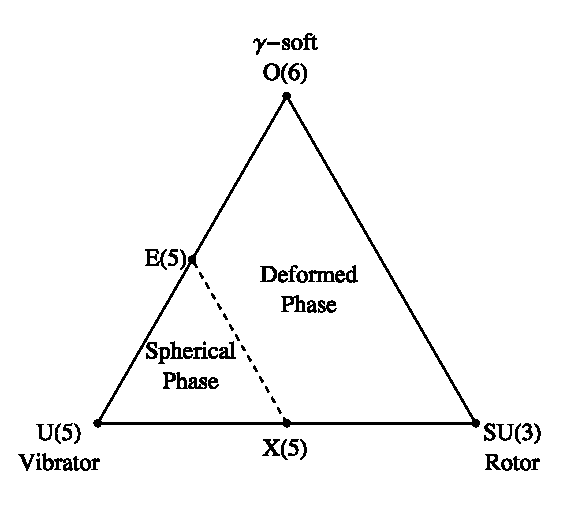
\includegraphics[scale=1]{Discussion/CastenTriangle.eps}
    \caption{The interacting boson model symmetry triangle. The critical point symmetries described by Iachello\citep{iachello00:_x5} are marked.}
    \label{fig:castentriangle}
\end{figure}

\section{Dynamic Moments of Inertia}
\label{sec:Dynamic}

Identical bands in neighboring nuclei are a phenomenon that was discovered in the 1990s \citep{baktash95:_dynamic_inertia}. These identical bands indicate identical moments of inertia in two different nuclei. Baktash\citep{baktash95:_dynamic_inertia} defines two different moments of inertia: kinematic ($\mathscr{J}^{(1)}$) and dynamic ($\mathscr{J}^{(2)}$), specifically identifying $\mathscr{J}^{(2)}$ as being identical in both bands. These moments of inertia can be approximated for rotational bands as 
\begin{equation}
    \begin{split}
        \mathscr{J}^{(1)}\equiv I/\omega \approx 2I/E_{\gamma} \\
        \mathscr{J}^{(2)}\equiv (d^2E/dI^2)^{-1} = dI/d\omega \approx 4/\delta E_{\gamma}
    \end{split}
\end{equation}
where $I$ is the spin of the level being depopulated, $E_{\gamma}$ is the energy of the gamma depopulating level $I$, $\delta E_{\gamma}$ is the difference between two separate energies of gamma transitions, and $\omega$ us the rotational frequency such that 
\begin{equation}
    \hbar \omega(I) =dE_{I}/dI \approx \left[E(I+1)-E(I-1)\right]/2 = E_{\gamma}(I+1)/2
\end{equation}
As $\mathscr{J}^{(2)}$ is a derivative of the spin, it eliminates any single particle component of the aligned angular momentum, making it a better indicator if the collective properties of the band. There is still a slowly changing component that is seen with increasing spin.

While Baktash discussed the identical band phenomenon between two different nuclei, it can also be used to compare bands within the same nucleus, giving insight into the relative nature of the collective bands \citep{aprahamian18:_156gd}. Combining the dynamic moment of inertia with measures of the $\rho^2$ of E0 transitions can give further insight into the nuclear matrix element. While the E0 matrix element is generally seen as a change in the radius of the nucleus between two states of the same $J^{\pi}$, it is, more accurately, a combination of this radial change and a measure of the overlap of the nuclear states. Comparing the dynamic moments of inertia of the two bands involved in an E0 transition can aid in examining the strength of the nuclear overlap.

To examine the structure of the bands seen in this experiment, the dynamic moments of inertia can be compared. This is usually done with higher spins, but examination at lower spins can allow for more bands to be compared. The energy difference tracks linearly, with the slope being directly correlated to the moment of inertia of the band, as seen in Figures \ref{fig:154_Dynamic}, \ref{fig:154_Dynamic0}, \ref{fig:156_Dynamic}, and \ref{fig:156_Dynamic0}. The slopes of these bands are summarized in Tables \ref{tab:154_Dynamic} and \ref{tab:156_Dynamic}. Slopes will vary with spin, and slopes with an error had enough points to calculate the error on the slope based on the fit. Those without error had only two points or, in the case of the second excited $2^+$ band, one point and the origin. These points each require two levels of the band to be known for calculation. The intercept was left to float, but not included, as it was in agreement with 0 in all cases where error could be calculated.

\section{$^{154}$Gd Results}
\label{sec:154_Discussion}
In Chapter \ref{chap:154Gd}, the results of this work on the nucleus $^{154}$Gd were detailed. From the singles data multipole assignments were confirmed for two transitions, conversion coefficiencts were measured for 30 transitions, and $\delta$ was measured for one. A new transition, from $5^-_{0^-}\rightarrow 6^+_{gs}$ was seen. Five pure E0 transitions were measured via coincidence (Table \ref{tab:154Gd_0_to_0}), with two of these transitions having been measured for the first time in this work ($0^+_6\rightarrow 0^+_2$ and $0^+_7\rightarrow 0^+_3$). None of these $0^+$ states had lifetimes, but the $q_K^2(E0/E2)$ value was calculated for all the transitions (Table \ref{tab:154Gd_E0_0}).

A total of 22 $J^{\pi}\rightarrow J^{\pi}$ transitions were measured for $2^+$ (Table \ref{tab:154Gd_2_to_2}), $4^+$ (Table \ref{tab:154Gd_4_to_4}), and $6^+$ (Table \ref{tab:154Gd_6_to_6}) states, 11 of these transitions for the first time. Of these 22 transitions, 11 have conversion coefficients indicating evidence of E0 components. Four of these transitions had known $\delta$ mixing ratios, allowing for the calculation of $\epsilon$, the E0/E2 mixing ratio (Table \ref{tab:154Gd_E0_d}), and in two cases with known lifetimes, the nuclear strength parameter $\rho^2(E0)$. For the rest of the transitions, $\delta$ was assumed to be 1, so $q^2\alpha(E2)$ and B(E0) ratios were calculated for transitions depopulating the same level (Tables \ref{tab:154Gd_E0} and \ref{tab:154Gd_BE0_Comp}). Combining these ratios with the dynamic moments of inertia can give some insight into the strength of $\rho^2(E0)$.

\begin{figure}[!]
    \begin{subfigure}{\textwidth}
    \centering
    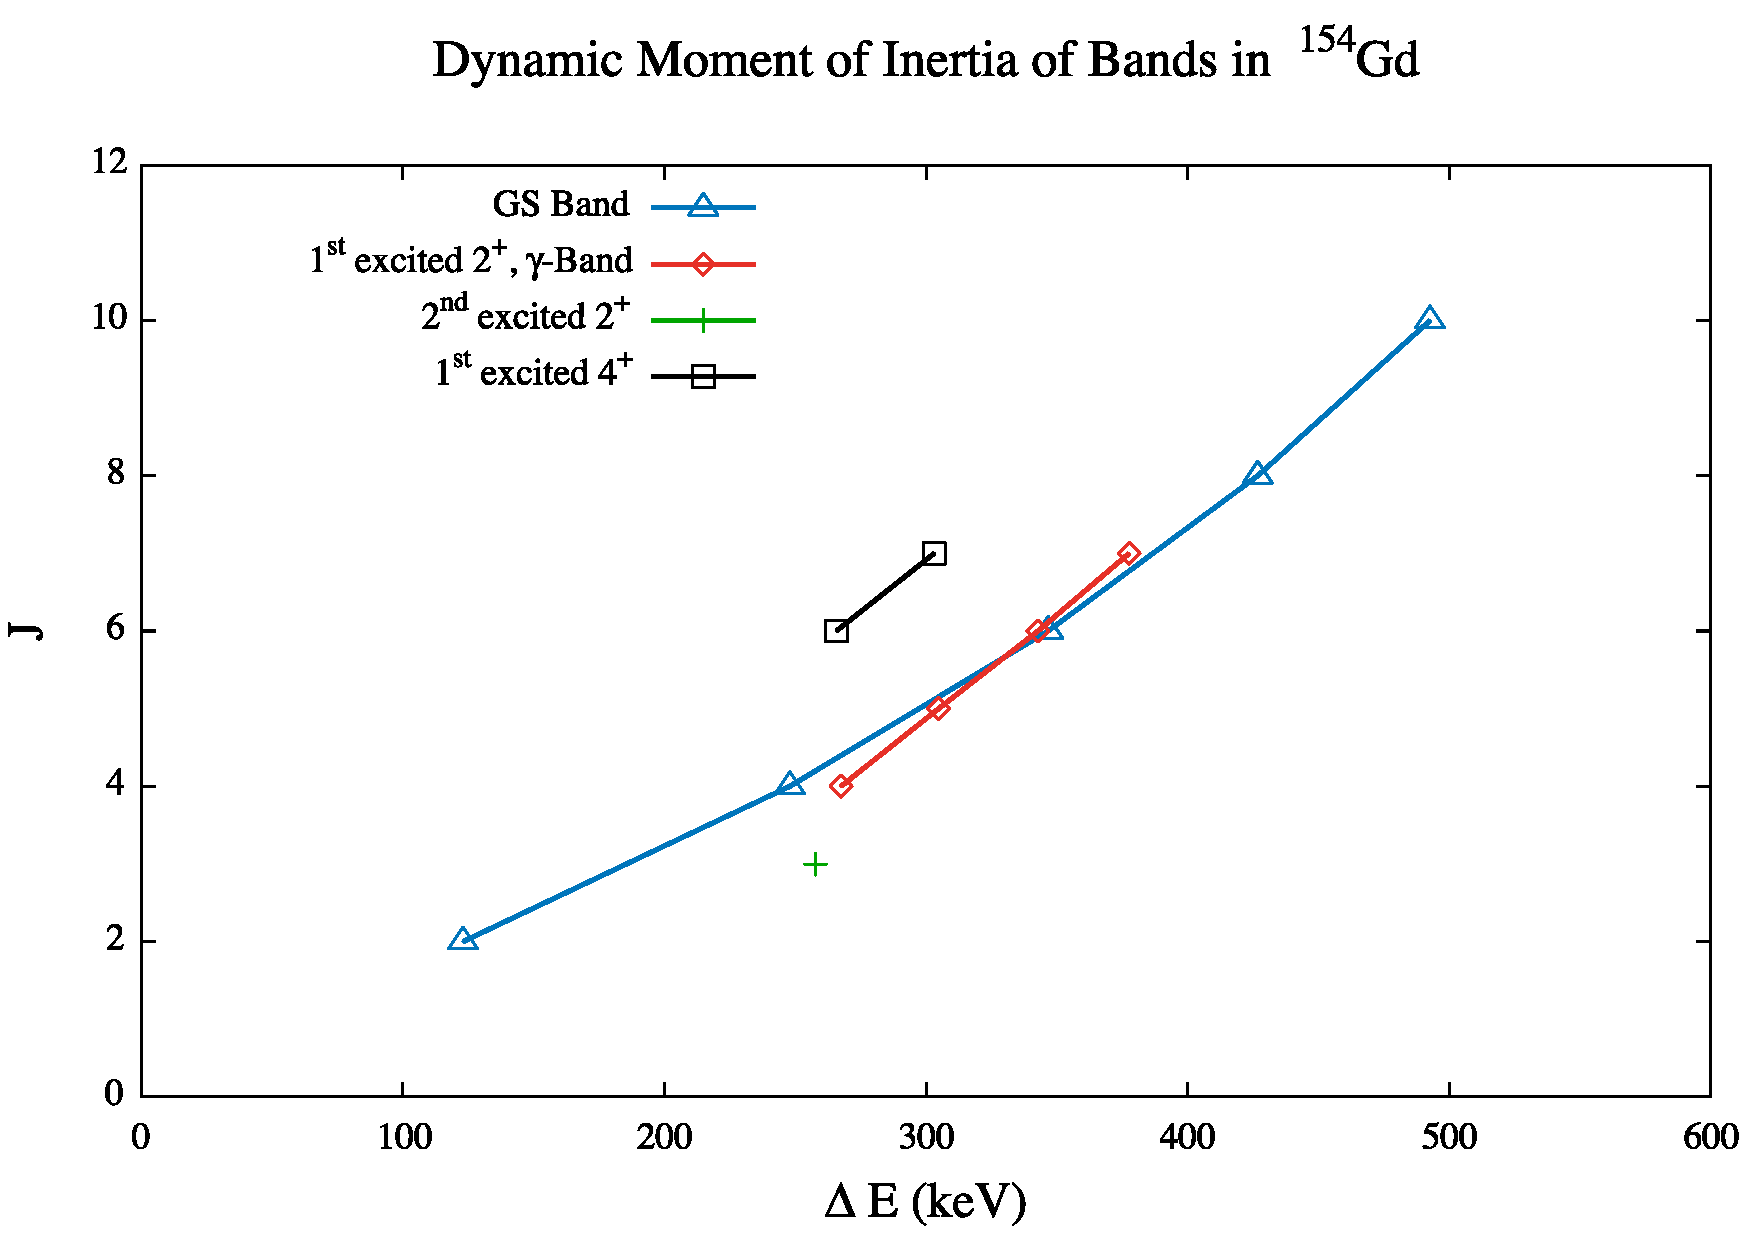
\includegraphics[scale=0.4]{Discussion/154_Dynamic.pdf}
    \caption*{(a)}
    \end{subfigure}
    \begin{subfigure}{\textwidth}
    \centering
    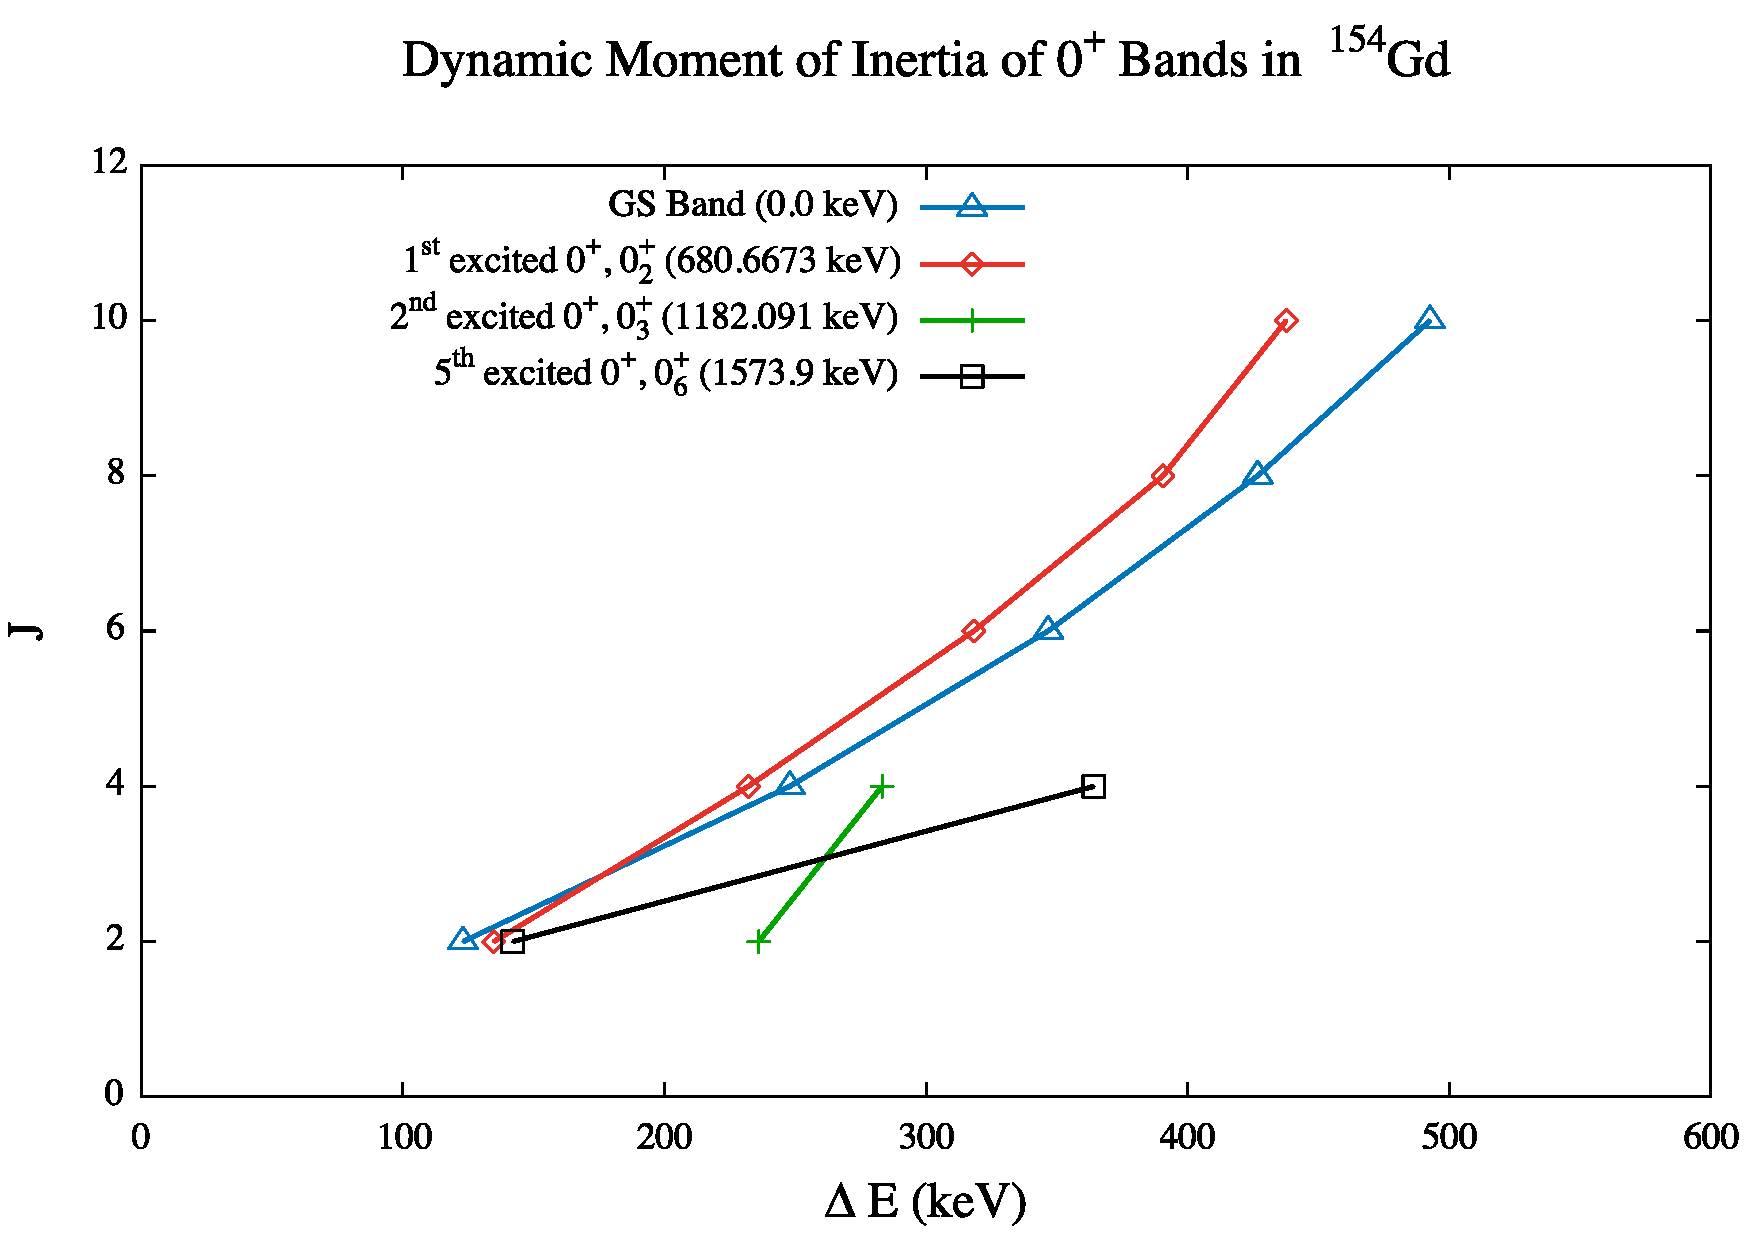
\includegraphics[scale=0.4]{Discussion/154_Dynamic0.pdf}
    \caption*{(b)}
    \end{subfigure}
    \caption{(a) The dynamic moments of inertia of the ground state, $K=2^+_1$ and $K=4^+_1$ bands. As is seen visually and with the slopes, the ground state band and the $\gamma$ band have similar moments of inertia and the $K=2^+_1$ and $K=4^+_1$ bands have identical moments of inertia. (b) The dynamic moments of inertia of the four $0^+$ bands seen in the experiment. The ground state band and the first excited $0^+$ band have very similar moments of inertia, while the second and fifth $0^+$ bands differ greatly.}
    \label{fig:154_Dynamic}
\end{figure}

\begin{figure}[!]
    \centering
    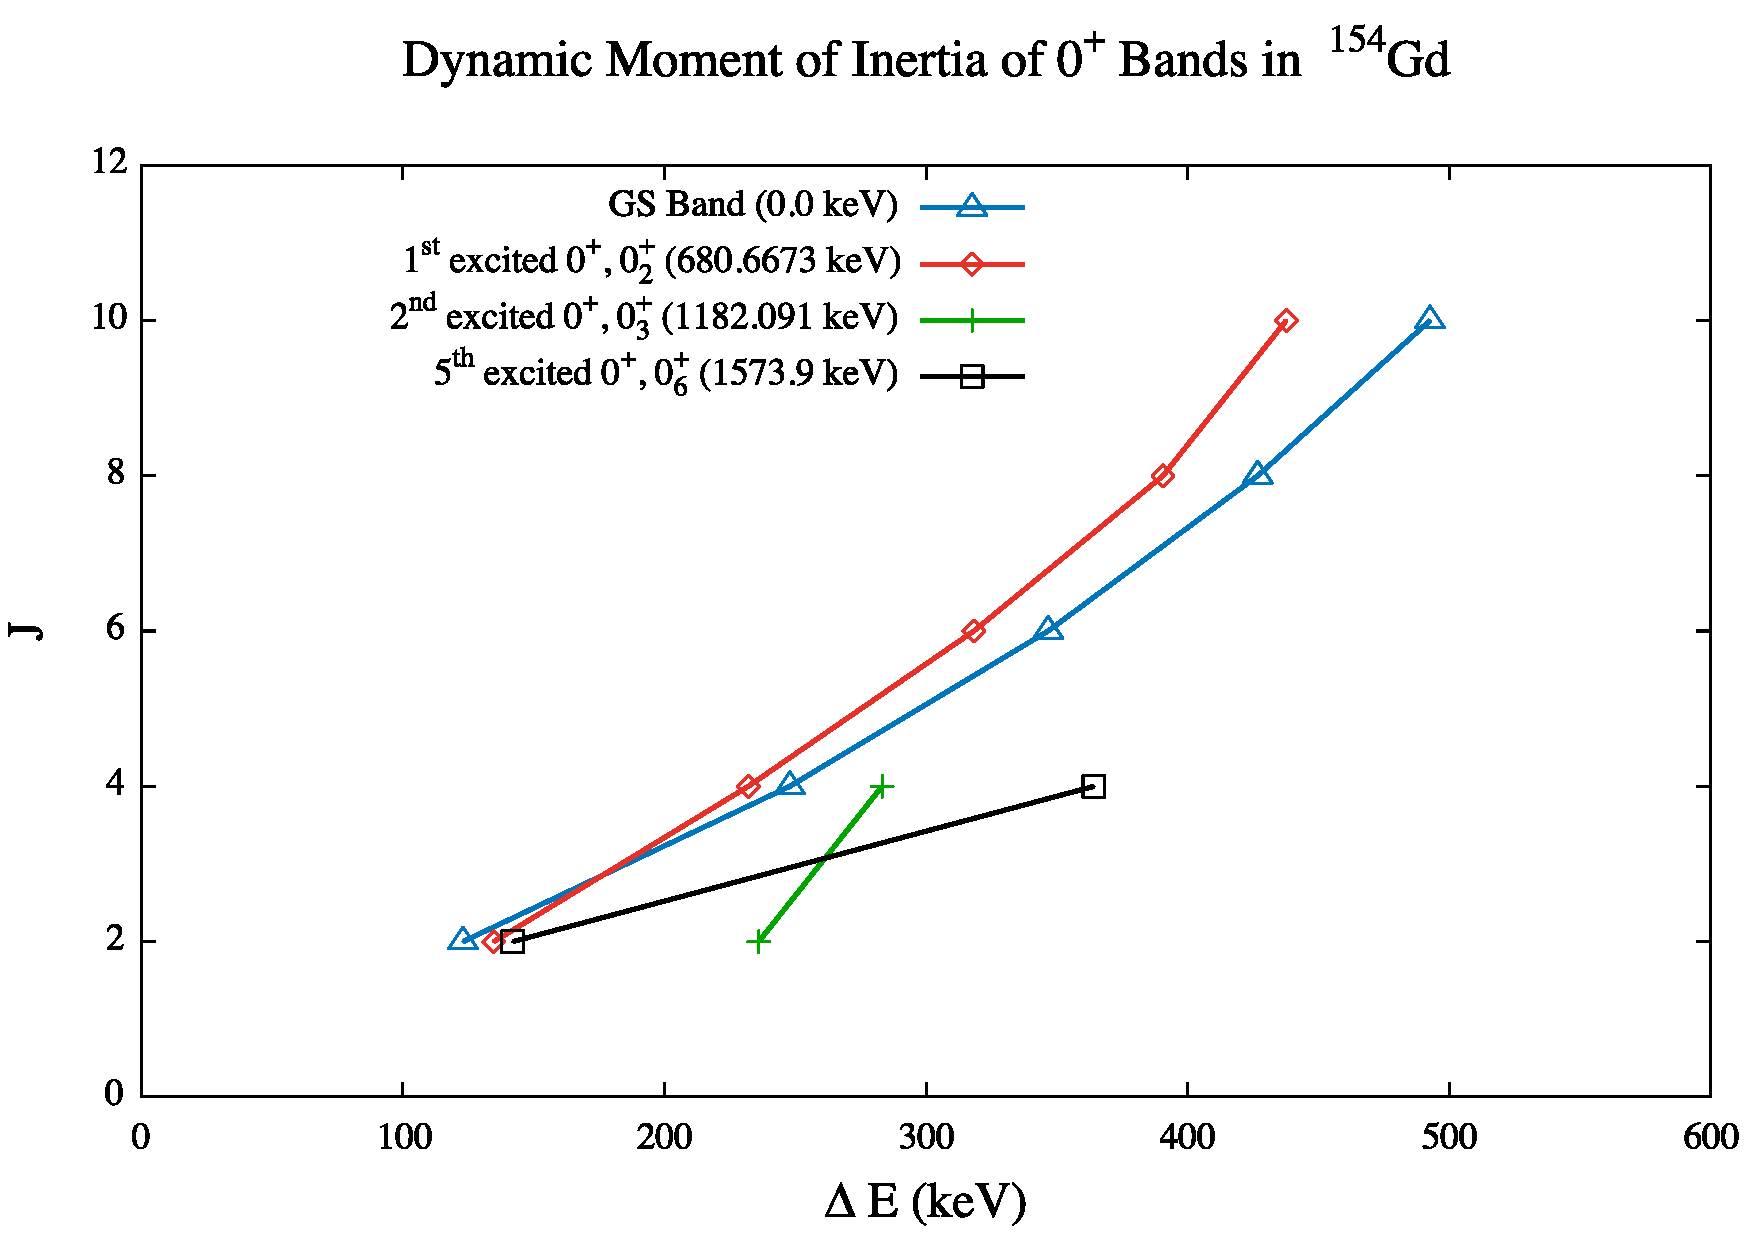
\includegraphics[scale=0.45]{Discussion/154_Dynamic0.pdf}
    \caption{The dynamic moments of inertia of the four $0^+$ bands seen in the experiment. As is seen visually and with the slopes, the ground state band and the first excited $0^+$ band have very similar moments of inertia.}
    \label{fig:154_Dynamic0}
\end{figure}

\begin{table}[!]
    \centering
    \caption{Dynamic Moments of Inertia of Bands seen in $^{154}$Gd}
    \begin{tabular}{c|c}
        \toprule
        Band & Moment of Inertia  \\
        \hline
        Ground State & 0.0214 (15) \\
        1st excited $0^+$, $0^+_2$ & 0.0258 (19) \\
        2nd excited $0^+$, $0^+_3$ & 0.0424 \\
        5th excited $0^+$, $0^+_6$ & 0.0090 \\
        1st excited $2^+$, $\gamma$-band & 0.0271 (3) \\
        2nd excited $2^+$ & 0.0155 \\
        1st excited $4^+$ & 0.0267 \\
        \bottomrule
    \end{tabular}
    \\[2pt]
    \footnotesize
    \label{tab:154_Dynamic}
    Table \ref{tab:154_Dynamic}: List of the moments of inertia of the bands seen in $^{154}$Gd in this experiment. The moment of inertia is the slope in a least-squares linear regression. Those without error only had one or two points of energy difference, so the standard deviation of the slope could not be calculated. The ground state band the the first excited $0^+$ band agree within two standard deviations.
\end{table}

The $\gamma$-band, seen in Figure \ref{fig:154_Dynamic} is a vibration built on the ground state, leading to a nearly identical dynamic moment of inertia. The $K=4^+$ band has a nearly identical moment of inertia to the $\gamma$-band, indicating it, too, may be a vibration built on the same structure as the ground state. The first excited $0^+$ state $0^+_2$, seen in Figure \ref{fig:154_Dynamic0}, agrees with the $\gamma$-band within $1\sigma$. The variation in the error of slopes has to do with the slow change in $\mathcal{J}^{(2)}$ due to the increase in spin. 

\subsection{$K^{\pi}=0^+_2$, First Excited $0^+$ Band, 680.6673 keV}

The conversion coefficients for the singles and gated data originating from the first excited $0^+$ band are in Tables \ref{tab:154Gd_Single_02_Disc} and \ref{tab:154Gd_02_Gate_Disc}, respectively. The first excited $0^+$ band is the only band with lifetimes and mixing ratios such that $\rho^2$ could be calculated, seen in Table \ref{tab:154Gd_E0_0}. The first excited $0^+$ band has a very similar slope to the ground state band, as seen both in Figure \ref{fig:154_Dynamic0} and Table \ref{tab:154_Dynamic}, indicating similar moments of inertia. Lifetimes beyond the $4^+$ state are unknown, so the $\rho^2$ value cannot be calculated for the $6^+$ state, but could be calculated for the $2^+$ and $4^+$ states. With the large $\rho^2$ values calculated for the $2^+_{0^+_2}\rightarrow 2^+_{gs}$ and $4^+_{0^+_2}\rightarrow 4^+_{gs}$ transitions to the ground state, the small change in the moment of inertia would indicate a large overlap in the nuclear states. 

\begin{table}
    \centering
    \caption{$^{154}$Gd $K_i=0^+_2$ Internal Conversion Coefficients from Singles}
    \label{tab:154Gd_Single_02_Disc}
\begin{ThreePartTable}
    \begin{subtable}{\textwidth}
        \caption{}
    \begin{tabular}{c|c|c|c|c|c|c}
        \toprule
        $E$ (keV)	&	$J^{\pi}	\rightarrow	J^{\pi}$	&	$E_i$ (keV)	&	$E_f$ (keV)	&	$T_{1/2}$ (fs)	&	Multipolarity	&	$\delta$\\
        \hline
        557.58	&	$0^+_{0^+_2}	\rightarrow	2^+_{gs}$	&	680.6673	&	123.0709	&	4560	&	E2	&		\\
        \hline
        444.19	&	$2^+_{0^+_2}	\rightarrow	4^+_{\gamma}$	&	815.4917	&	370.9998	&	6400	&	E2	&		\\
        \hline
        693.47	&	$2^+_{0^+_2}	\rightarrow	2^+_{gs}$	&	815.4917	&	123.0709	&	6400	&	E2+M1+E0	&	7.5 (4)	\\
        \hline
        232.44	&	$4^+_{0^+_2}	\rightarrow	2^+_{0^+_2}$	&	1047.592	&	815.4917	&	7600	&	E2	&	\\
	    &				&		&		&		&		& \\
	    \hline
        329.49	&	$4^+_{0^+_2}	\rightarrow	6^+_{gs}$	&	1047.592	&	717.662	&	7600	&	E2	&	\\
        \hline

        676.70	&	$4^+_{0^+_2}	\rightarrow	4^+_{gs}$	&	1047.592	&	370.9998	&	7600	&	E0+M1+E2	&	+2.9 (4)	\\
        \hline
        924.85	&	$4^+_{0^+_2}	\rightarrow	2^+_{gs}$	&	1047.592	&	123.0709	&	7600	&	E2	&	\\
        \hline        
        610.71	&	$8^+_{0^+_2}	\rightarrow	8^+_{gs}$	&	1756.49	&	1144.44	&		&	E0+M1+E2	&	-0.69 (14)	\\
	    &				&		&		&		&		&	\\
	    \bottomrule
    \end{tabular}
    \end{subtable}
    \end{ThreePartTable}
\end{table}
\begin{table}
    \ContinuedFloat
    \begin{subtable}{\textwidth}
    \end{subtable}
    \begin{ThreePartTable}
    \begin{subtable}{\textwidth}
        \caption{}
        \begin{tabular}{c|c|c|c|c|c|c}
            \toprule
            $E$ (keV) & Shell &	$\alpha$ (This Work)	&	$\alpha$  (Theory)\citep{kibedi08:_BRICC}	&	$\alpha$ (Spits)\citep{spits96:_154gd} & $\alpha$ (Gono)\citep{gono74:_154gd_e0}	& $\epsilon^2$ (This Work)	\\
            \hline
            557.58	& K &	0.0486	(42) (6)	&	0.00864 (12)	&	0.009 (1) & 0.0091 (16)	& \\
            \hline
            444.19	& K &	0.0525	(32) (6)	&	0.01543 (22)	&	0.014 (1)&	\\
            \hline
            693.47	& K &	0.0017	(2) (1)	&	0.00522 (8)	&	0.0421 (4) &	\\
            \hline
            232.44	& K &	0.287	(103) $^{+83}_{-82}$	&	0.0982 (14)	&	0.100 (8)	& \\
            &	LM &		0.0450	(46) (13)	&	0.0288 (4)	&	&	\\
            \hline
            329.49	 & K &	0.1573	(89) (17)	&	0.0352 (5)	&	0.034 (3)	&\\
            \hline
            676.70	& K &	0.0283	(4) (10)	&	0.00593 (17)	&	0.0460 (46) & 0.040 (7)	& 0.1762 (244) (62)\\
            \hline
            924.85	& K &	0.0033	(9) (1)	&	0.00273 (4)	&	0.0031 (1)	&\\
            \hline
            610.71	& K &	0.0258	(10) (7)	&	0.0110 (6)	& &	0.053 (7)	& 0.0250 (52) (7)\\
            		& L &	0.0167	(9) (4)	&	0.00158 (7)	&	&	& 0.0227 (48) (5) \\
            \bottomrule
        \end{tabular}
        \end{subtable}

        \makeatletter\def\TPT@hsize{}\makeatletter
        
        \begin{tablenotes}[para,flushleft]
            Table \ref{tab:154Gd_Single_02_Disc}: A list of conversion coefficients from $^{154}$Gd, originating in the $K_i=0^+_2$ band. Table (a) lists transition information. Multipolarities and mixing ratios were taken from the nuclear data sheets\citep{reich09:_nds_154}. Table (b) lists the conversion coefficients. Unless otherwise stated, the $\alpha$ values are $\alpha_K$. An angular distribution correction has been applied based on multipolarities for pure transitions, and those with known mixing ratios. For transitions with an E0 component, the correction was applied assuming just the M1 and E2 components. The theory value is based on the listed multipolarity, also neglecting the E0 component in those cases. The $\epsilon^2$ values listed are for transitions with an E0 component possible, and a large enough $\alpha_{exp}$. The first error is statistical, the second is systematic. Numbers are compared with Spits et al.\citep{spits96:_154gd} and Gono et al.\citep{gono74:_154gd_e0}. The bands for each level are listed as subscripts.
        \end{tablenotes}
\end{ThreePartTable}
\end{table}


\begin{landscape}
\begin{table}
    \centering
    \caption{$J^{\pi}\rightarrow J^{\pi}$ Transitions for $K_i=0^+_2$ in $^{154}$Gd}
    \label{tab:154Gd_02_Gate_Disc}
\begin{ThreePartTable}
    \begin{subtable}{\textwidth}
        \caption{}
    \begin{tabular}{c|c|c|c|c|c}
        \toprule
        $E_i$ (keV)	& $J^{\pi}_i$ &	$E_f$ (keV)	& $J^{\pi}_f$ & $E$ (keV)	&	Gate \\
        \hline
        815.4917 & $2^+_{0^+_2}$ & 123.0709 & $2^+_{gs}$ & 692.4205 & 123.0706\\ \hline
        1047.592 & $4^+_{0^+_2}$ & 370.9998 & $4^+_{gs}$ &  676.593 & 247.9288 \\\hline
        1365.878 & $6^+_{0^+_2}$ & 717.662 & $6^+_{gs}$ & 648.3 & 346.643 \\
	    \bottomrule
    \end{tabular}
    \end{subtable}
    \end{ThreePartTable}
\end{table}
\begin{table}
    \centering
    \ContinuedFloat
    \begin{subtable}{\textwidth}
    \end{subtable}
    \begin{ThreePartTable}
    \begin{subtable}{\textwidth}
        \begin{tabular}{c|c|c|c|c|c|c}
            \multicolumn{7}{c}{TABLE 6.3 (CONTINUED)} \\
            \multicolumn{7}{c}{(b)} \\
            \toprule
            & \multicolumn{5}{c|}{$\alpha$}	& 	\\ 
             &	& \multicolumn{2}{c|}{Theory\citep{kibedi08:_BRICC}}	& & 	\\ 
            $E_i$ (keV)	&This Work	& $\alpha$(M1) & $\alpha$(E2) &	Spits\citep{spits96:_154gd} & Gono\citep{gono74:_154gd_e0} & $\epsilon^2$ (This Work)	\\
            \hline
            815.4917 &  0.0430 (3)(9) & 0.00952 (14) & 0.00516 (8) &  0.0421 (4) & & 1.9233 (1035)(402)\\ \hline
            1047.592 & 0.0550 (2)$^{+12}_{-11}$ & 0.01007 (15) & 0.00544 (8) & 0.0460 (46) & 0.040 (7) & 0.4274 (590)$^{+93}_{-85}$\\
            &   0.0131 (1)(3) & 0.001384 (20) & 0.000870 (13) & & & 0.1108 (153)(25)\\ \hline
            1365.878  & 0.0778 (4)(16) & 0.01120 (16) & 0.00601 (9) & & 0.039 (7) & 0.1017 (206)(21)\\
            \bottomrule
        \end{tabular}
        \end{subtable}

        \makeatletter\def\TPT@hsize{}\makeatletter
        
        \begin{tablenotes}[para,flushleft]
            Table \ref{tab:154Gd_02_Gate_Disc}: A list of conversion coefficients from $^{154}$Gd for $J^{\pi}\rightarrow J^{\pi}$ transitions for $K_i=0^+_2$ seen in the gated data. The first error is statistical, the second is systematic. Numbers are compared with theoretical K-shell conversion coefficients for M1 and E2 transitions, as well as results from Spits et al.\citep{spits96:_154gd} and Gono et al.\citep{gono74:_154gd_e0}. The $\epsilon^2$ values listed are for transitions with a large enough $\alpha_{exp}$ to indicate an E0 component. All coefficients are K-electrons, except for the transition from 1047 keV. The second value is the LM peak.
        \end{tablenotes}
\end{ThreePartTable}
\end{table}
\end{landscape}


The similarity in the dynamic moment of inertia, coupled with the large $\rho^2$ values, indicate a $\beta$-vibration. The $\gamma$-vibration band dynamic moment of inertia behaves very similarly to the ground state in much the same way, also favoring this interpretation. 

\subsection{$K^{\pi}=0^+_3$, Second Excited $0^+$ Band, 1182.091 keV}

The conversion coefficients for the gated data originating from the second excited $0^+$ band are in Table \ref{tab:154Gd_03_Gate_Disc}. All of the measurements from the $K=0^+_3$ band were limits, and connected to either the $0^+_2$ band or the $\gamma$-band. All the transitions were measured with two different gates. The $2^+$ state transitions only had lower limits, with the lower limit on the $\gamma$-band indicating an E0 component. For the $4^+$ state transitions, the limits were upper limits. The upper limit to the $0^+_2$ transition indicated little to no E0 component, while the upper limit on the transition to the $\gamma$-band allows for a larger E0 component. The transitions, in agreement with Table \ref{tab:154Gd_BE0_Comp}, indicate the $0^+_3$ band favors populating the $\gamma$-band. This band also has a much larger dynamic moment of inertia, compared to the ground state, first excited $0^+$ state and $\gamma$-bands. None of the transitions examined have known mixing ratios, so the $q^2$ and $\alpha q^2$ can be found in Tables \ref{tab:154Gd_E0} and \ref{tab:154Gd_E0_0}. 

\begin{landscape}
    \footnotesize
    \begin{longtable}{>{\footnotesize}c|>{\footnotesize}c|>{\footnotesize}c|>{\footnotesize}c|>{\footnotesize}c|>{\footnotesize}c|>{\footnotesize}c|>{\footnotesize}c|>{\footnotesize}c|>{\footnotesize}c|>{\footnotesize}c}
        \caption{$J^{\pi}\rightarrow J^{\pi}$ Transitions for $K_i=0^+_3$ in $^{154}$Gd}
        \label{tab:154Gd_03_Gate_Disc}\\
        \toprule
        &	& & & 	&  &	& \multicolumn{2}{>{\footnotesize}c|}{Theory\citep{kibedi08:_BRICC}}	& 	\\ 
        $E_i$ (keV)	& $J^{\pi}_i$ &	$E_f$ (keV)	& $J^{\pi}_f$ & $E$ (keV)	&	Gate &		$\alpha$ (This Work)	& $\alpha$(M1) & $\alpha$(E2) &	$\alpha$ (Spits)\citep{spits96:_154gd} & $\epsilon^2$ (This Work)\\
        \hline
        \endfirsthead
        \caption[]{$J^{\pi}\rightarrow J^{\pi}$ Transitions for $K_i=0^+_3$ in $^{154}$Gd}\\
        \toprule
        &	& & &	&  &	& \multicolumn{2}{>{\footnotesize}c|}{Theory\citep{kibedi08:_BRICC}}	&	\\ 
        $E_i$ (keV)	& $J^{\pi}_i$ &	$E_f$ (keV)	& $J^{\pi}_f$ & $E$ (keV)	&	Gate &		$\alpha$ (This Work)	& $\alpha$(M1) & $\alpha$(E2) &	$\alpha$ (Spits)\citep{spits96:_154gd} & $\epsilon^2$ (This Work)\\
        \hline
	    \endhead
	    \endfoot
        \multicolumn{11}{p{1.4\textwidth}}{Table \ref{tab:154Gd_03_Gate_Disc}: A list of conversion coefficients from $^{154}$Gd for $J^{\pi}\rightarrow J^{\pi}$ transitions for $K_i=0^+_3$ seen in the gated data. The first error is statistical, the second is systematic. Numbers are compared with theoretical K-shell conversion coefficients for M1 and E2 transitions, as well as results from Spits et al.\citep{spits96:_154gd}. The $\epsilon^2$ values listed are for transitions with a large enough $\alpha_{exp}$, and assumed to be pure E2 transitions, to give a minimum $\epsilon^2$. For $\alpha_{exp}$ that are upper limits and $0^+\rightarrow 0^+$ transitions, $\epsilon^2$ is not listed. All coefficients are K-electrons.}
        \endlastfoot
        1182.091 & $0^+_3$ & 680.6673 & $0^+_2$ &  501.427 & 557.581 & $>0.0283$ & 0.0213 (3) & 0.01126 (16) & $>0.2$ & \\\hline
        1418.16 & $2^+_{0^+_3}$ & 815.4917 & $2^+_{0^+_2}$ & 602.688 &  692.4205 & $>0.0125$ & 0.01343 (19) & 0.00715 (10) & 0.025 (3)  & $>0.0054$\\
        &  & &  &  & 444.4924 & $>0.0093$ &  & & & $>0.0022$\\ \hline
        1418.16 &  $2^+_{0^+_3}$ & 996.2568 &  $2^+_{\gamma}$ & 421.893 & 873.1834 & $>0.0367$ & 0.0332 (5) & 0.01170 (25) & 0.114 (16) & $>0.0250$\\
        &  & &  &  & 625.2556 & $>0.0463$ & & & & $>0.0346$\\ \hline
        1701.39 & $4^+_{0^+_3}$ & 1047.592 & $4^+_{0^+_2}$ & 653.7 & 676.593 & $<0.0093$ & 0.01097 (16) & 0.00590 (9) & 0.0220 (62)  & \\
        &  & &  &  & 924.55 & $<0.0301$ & & & &\\ \hline
        1701.39 & $4^+_{0^+_3}$ & 1263.778 & $4^+_{\gamma}$ & 437.612 & 892.775 & $<0.0585$ & 0.0302 (5) & 0.01605 (23) &  & \\
        &  & &  &  & 1140.702 & $<0.0511$ & & &  & \\ 
        \bottomrule
    \end{longtable}
\end{landscape}

\subsection{$K^{\pi}=0^+_6$, Fifth Excited $0^+$ Band, 1573.9 keV}

The conversion coefficients for the singles and gated data originating from the fifth excited $0^+$ band are in Tables \ref{tab:154Gd_Single_06_Disc} and \ref{tab:154Gd_06_Gate_Disc}, respectively. Transitions between the $0^+_6$ band and the $0^+_2$ and $0^+_3$ bands could be seen in the gates, specifically for the $0^+$ states. $\rho^2$ could not be calculated due to a lack of lifetime, but the two transitions could be compared, in Table \ref{tab:154Gd_BE0_Comp}, indicating a stronger connection to the $0^+_3$ band. Comparisons between the $0^+_2$ and $\gamma$-band were also done using the $2^+$ state, generally indicating a stronger connection to the $\gamma$-band than the $0^+_2$ band. None of the transitions examined have known mixing ratios, so the $q^2$ and $\alpha q^2$ can be found in Tables \ref{tab:154Gd_E0} and \ref{tab:154Gd_E0_0}. The fifth excited $0^+$ band has the smallest slope of all the bands looked at in this nucleus, the strongly different moment of inertia gives an indication this band is likely not built on the $\gamma$-band or $0^+_2$ band.

\begin{table}
    \centering
    \caption{$^{154}$Gd $K_i=0^+_6$, Internal Conversion Coefficients from Singles}
    \label{tab:154Gd_Single_06_Disc}
\begin{ThreePartTable}
    \begin{subtable}{\textwidth}
        \caption{}
    \begin{tabular}{c|c|c|c|c|c|c}
        \toprule
        $E$ (keV)	&	$J^{\pi}	\rightarrow	J^{\pi}$	&	$E_i$ (keV)	&	$E_f$ (keV)	&	$T_{1/2}$ (fs)	&	Multipolarity	&	$\delta$\\
        \hline
        416.79	&	$4^+_{0^+_6}	\rightarrow	3^+_{2^+}$	&	2080.23	&	1660.903	&		&	(M1)	&	\\
        \bottomrule
    \end{tabular}
    \end{subtable}
    \end{ThreePartTable}
\end{table}
\begin{table}
    \ContinuedFloat
    \begin{subtable}{\textwidth}
    \end{subtable}
    \begin{ThreePartTable}
    \begin{subtable}{\textwidth}
        \caption{}
        \begin{tabular}{c|c|c|c|c|c}
            \toprule
            $E$ (keV) & Shell &	$\alpha$ (This Work)	&	$\alpha$  (Th)\citep{kibedi08:_BRICC}	&	$\alpha$ (Spits)\citep{spits96:_154gd} & $\alpha$ (Gono)\citep{gono74:_154gd_e0}		\\
            \hline
            416.79	 & K &	0.0334	(47) (6)	&	0.03442 (5)	&	\\
            \bottomrule
        \end{tabular}
        \end{subtable}
        \begin{tablenotes}[para]
            Table \ref{tab:154Gd_Single_06_Disc}: A list of conversion coefficients from $^{154}$Gd, originating in the $K_i=0^+_6$ band. Table (a) lists transition information. Multipolarities and mixing ratios were taken from the nuclear data sheets\citep{reich09:_nds_154}. Table (b) lists the conversion coefficients. Unless otherwise stated, the $\alpha$ values are $\alpha_K$. An angular distribution correction has been applied based on multipolarities for pure transitions, and those with known mixing ratios. The first error is statistical, the second is systematic. Numbers are compared with Spits et al.\citep{spits96:_154gd} and Gono et al.\citep{gono74:_154gd_e0} The starred value was used as an absolute calibration of the conversion electron detector in the Gono work. The bands for each level are listed as subscripts.
        \end{tablenotes}
\end{ThreePartTable}
\end{table}


\begin{landscape}
    \footnotesize
    \begin{longtable}{>{\footnotesize}c|>{\footnotesize}c|>{\footnotesize}c|>{\footnotesize}c|>{\footnotesize}c|>{\footnotesize}c|>{\footnotesize}c|>{\footnotesize}c|>{\footnotesize}c|>{\footnotesize}c|>{\footnotesize}c}
        \caption{$J^{\pi}\rightarrow J^{\pi}$ Transitions for $K_i=0^+_6$ in $^{154}$Gd}
        \label{tab:154Gd_06_Gate_Disc}\\
        \toprule
        &	& & & 	&  &	& \multicolumn{2}{>{\footnotesize}c|}{Theory\citep{kibedi08:_BRICC}}	& 	\\ 
        $E_i$ (keV)	& $J^{\pi}_i$ &	$E_f$ (keV)	& $J^{\pi}_f$ & $E$ (keV)	&	Gate &		$\alpha$ (This Work)	& $\alpha$(M1) & $\alpha$(E2) &	$\alpha$ (Spits)\citep{spits96:_154gd} & $\epsilon^2$ (This Work)\\
        \hline
        \endfirsthead
        \caption[]{$J^{\pi}\rightarrow J^{\pi}$ Transitions for $K_i=0^+_6$ in $^{154}$Gd}\\
        \toprule
        &	& & &	&  &	& \multicolumn{2}{>{\footnotesize}c|}{Theory\citep{kibedi08:_BRICC}}	& 	\\ 
        $E_i$ (keV)	& $J^{\pi}_i$ &	$E_f$ (keV)	& $J^{\pi}_f$ & $E$ (keV)	&	Gate &		$\alpha$ (This Work)	& $\alpha$(M1) & $\alpha$(E2) &	$\alpha$ (Spits)\citep{spits96:_154gd} & $\epsilon^2$ (This Work)\\
        \hline
	    \endhead
	    \endfoot
        \multicolumn{11}{p{1.4\textwidth}}{Table \ref{tab:154Gd_06_Gate_Disc}: A list of conversion coefficients from $^{154}$Gd for $J^{\pi}\rightarrow J^{\pi}$ transitions for $K_i=0^+_6$ seen in the gated data. The first error is statistical, the second is systematic. Numbers are compared with theoretical K-shell conversion coefficients for M1 and E2 transitions, as well as results from Spits et al.\citep{spits96:_154gd}. The $\epsilon^2$ values listed are for transitions with a large enough $\alpha_{exp}$, and assumed to be pure E2 transitions, to give a minimum $\epsilon^2$,a lower limit. For $\alpha_{exp}$ that are upper limits, $\epsilon^2$ is not listed. No $\epsilon^2$ is indicated for the $0^+\rightarrow 0^+$ transitions. All coefficients are K-electrons, except for the transition from 1047 keV. The second value is the LM peak.}
        \endlastfoot
        1573.9 & $0^+_6$ & 680.6673 & $0^+_2$ &  893.9 & 557.581 & $>0.0183$ & 0.00510 (8) & 0.00294 (5) & &\\\hline
        1573.9 & $0^+_6$ & 1182.091 & $0^+_3$ & 391.9 &  1059.033 & $>0.0529$ & 0.0402 (6) & 0.0216 (3) & $>0.1$ & \\\hline
        1716.050 & $2^+_{0^+_2}$ & 815.4917 & $2^+_{0^+_2}$ & 900.5583 &  692.4205 & $<0.0105$ & 0.00501 (7) & 0.00289 (4) & &  \\
        & & &  & & 444.4924 & $<0.0531$ & & &  & \\ \hline
        1716.050 & $2^+_{0^+_6}$ & 996.2568 & $2^+_{\gamma}$ & 719.80 & 873.1834 & 0.0113 (46)$^{+33}_{-25}$ & 0.00865 (13) & 0.00472 (7) & & $>0.0066$\\
        &  & &  &  & 625.2556 & 0.0501 (260)$^{+147}_{-113}$ & & &  & $>0.0454$\\ 
        \bottomrule
    \end{longtable}
\end{landscape}

\subsection{$K^{\pi}=0^+_7$, Sixth Excited $0^+$ Band, 1650.3 keV}

The conversion coefficients for the gated data originating from the sixth excited $0^+$ band are in Table \ref{tab:154Gd_03_Gate_Disc}. Transitions between the $0^+_7$ band and the $0^+_2$ and $0^+_3$ bands could be seen in the gates, specifically for the $0^+$ states. $\rho^2$ could not be calculated due to a lack of lifetime, but the two transitions could be compared, in Table \ref{tab:154Gd_BE0_Comp}, indicating a stronger connection to the $0^+_3$ band. Comparisons between the $0^+_2$ and $\gamma$-band were also done using the $2^+$ state, generally indicating a stronger connection to the $\gamma$-band than the $0^+_2$ band, although with this ratio being a limit, this could be untrue. None of the transitions examined have known mixing ratios, so the $q^2$ and $\alpha q^2$ can be found in Tables \ref{tab:154Gd_E0} and \ref{tab:154Gd_E0_0}. This band did not have enough information to calculate the dynamic moment of inertia, hence its omission from Figure \ref{fig:154_Dynamic0} and Table \ref{tab:154_Dynamic}.

\begin{landscape}
    \footnotesize
    \begin{longtable}{>{\footnotesize}c|>{\footnotesize}c|>{\footnotesize}c|>{\footnotesize}c|>{\footnotesize}c|>{\footnotesize}c|>{\footnotesize}c|>{\footnotesize}c|>{\footnotesize}c|>{\footnotesize}c|>{\footnotesize}c}
        \caption{$J^{\pi}\rightarrow J^{\pi}$ Transitions for $K_i=0^+_7$ in $^{154}$Gd}
        \label{tab:154Gd_07_Gate_Disc}\\
        \toprule
        &	& & & 	&  &	& \multicolumn{2}{>{\footnotesize}c|}{Theory\citep{kibedi08:_BRICC}}	& 	\\ 
        $E_i$ (keV)	& $J^{\pi}_i$ &	$E_f$ (keV)	& $J^{\pi}_f$ & $E$ (keV)	&	Gate &		$\alpha$ (This Work)	& $\alpha$(M1) & $\alpha$(E2) &	$\alpha$ (Spits)\citep{spits96:_154gd}& $\epsilon^2$ (This Work)\\
        \hline
        \endfirsthead
        \caption[]{$J^{\pi}\rightarrow J^{\pi}$ Transitions for $K_i=0^+_6$ in $^{154}$Gd}\\
        \toprule
        &	& & &	&  &	& \multicolumn{2}{>{\footnotesize}c|}{Theory\citep{kibedi08:_BRICC}}	& \\ 
        $E_i$ (keV)	& $J^{\pi}_i$ &	$E_f$ (keV)	& $J^{\pi}_f$ & $E$ (keV)	&	Gate &		$\alpha$ (This Work)	& $\alpha$(M1) & $\alpha$(E2) &	$\alpha$ (Spits)\citep{spits96:_154gd}& $\epsilon^2$ (This Work)\\
        \hline
	    \endhead
	    \endfoot
        \multicolumn{11}{p{1.4\textwidth}}{Table \ref{tab:154Gd_07_Gate_Disc}: A list of conversion coefficients from $^{154}$Gd for $J^{\pi}\rightarrow J^{\pi}$ transitions for $K_i=0^+_7$ seen in the gated data. The first error is statistical, the second is systematic. Numbers are compared with theoretical K-shell conversion coefficients for M1 and E2 transitions, as well as results from Spits et al.\citep{spits96:_154gd}. The $\epsilon^2$ values listed are for transitions with a large enough $\alpha_{exp}$, and assumed to be pure E2 transitions, to give a minimum $\epsilon^2$,a lower limit. For $\alpha_{exp}$ that are upper limits, $\epsilon^2$ is not listed. No $\epsilon^2$ is indicated for the $0^+\rightarrow 0^+$ transitions.All coefficients are K-electrons, except for the transition from 1047 keV. The second value is the LM peak.}
        \endlastfoot
        1650.3 & $0^+_7$ & 680.6673 & $0^+_2$ &  970.3 & 557.581 & $>0.0209$ & 0.00419 (6) & 0.00247 (4) & $>0.027$ \\ \hline
        1650.3 & $0^+_7$ & 1182.091 & $0^+_3$ & 468.3 &  1059.033 & $>0.0922$ & 0.0254 (4) & 0.01343 (19) & \\ \hline
        1775.429 & $2^+_{0^+_7}$ & 815.4917 & $2^+_{0^+_2}$ & 960.05 &  692.4205 & $>0.0221$ & 0.00430 (6) & 0.00253 (4) & & $>0.0196$ \\
        &  & & &  & 444.4924 & $>0.0231$ & & &  & $>0.0206$\\ \hline
        1775.429 & $2^+_{0^+_7}$ & 996.2568 & $2^+_{\gamma}$ & 779.165 & 873.1834 & 0.0206 (112)$^{+60}_{-46}$ & 0.00712 (10) & 0.00396 (6) & & $>0.0166$\\
        &  & &  &  & 625.2556 & 0.0745 (521)$^{+217}_{-165}$	& & & & $>0.0705$\\
        \bottomrule
    \end{longtable}
\end{landscape}

\subsection{$K^{\pi}=2^+$, $\gamma$ Band, 996.264 keV}

The conversion coefficients for the singles and gated data originating from the first excited $2^+$ band, the $\gamma$-vibrational band are in Tables \ref{tab:154Gd_Single_gamma_Disc} and \ref{tab:154Gd_gamma_Gate_Disc}, respectively. The $\gamma$ band has a very similar slope to the ground state band, as seen both in Figure \ref{fig:154_Dynamic} and Table \ref{tab:154_Dynamic}, indicating similar moments of inertia, although the slope is higher than that seen by the ground state band or first excited $0^+$ band. While measures of the transitions between the $\gamma$ band and ground state band could not be done in this work, measures between the $\gamma$-band and first excited $0^+$ were done. The $2^+\rightarrow2^+$ and $6^+\rightarrow6^+$ transitions indicate potentially large E0 components for the conversion coefficients. The $4^+\rightarrow4^+$ transition indicates small E0 components. Of these transitions, the $2^+\rightarrow2^+$ has a previously measured relative $\gamma$-intensity of 0.043 (6)\% \citep{reich09:_nds_154}. The low intensities of these transitions and the lack of mixing and branching ratios make it difficult to draw conclusions. None of the transitions examined have known mixing ratios, so the $q^2$ and $\alpha q^2$ can be found in Table \ref{tab:154Gd_E0}.

\begin{table}
    \centering
    \caption{$^{154}$Gd $K_i=2^+_1$, $\gamma$ Internal Conversion Coefficients from Singles}
    \label{tab:154Gd_Single_gamma_Disc}
\begin{ThreePartTable}
    \begin{subtable}{\textwidth}
        \caption{}
    \begin{tabular}{c|c|c|c|c|c|c}
        \toprule
        $E$ (keV)	&	$J^{\pi}	\rightarrow	J^{\pi}$	&	$E_i$ (keV)	&	$E_f$ (keV)	&	$T_{1/2}$ (fs)	&	Multipolarity	&	$\delta$\\
        \hline
        873.54	&	$2^+_{\gamma}	\rightarrow	2^+_{gs}$	&	996.2568	&	123.0709	&	950	&	E2+M1+E0	&	-9.4 (4)	\\
        \hline
        996.33	&	$2^+_{\gamma}	\rightarrow	0^+_{gs}$	&	996.2568	&	0	&	950	&	E2	&	\\
        \hline
        889.61	&	$6^+_{\gamma}	\rightarrow	6^+_{gs}$	&	1606.55	&	717.662	&		&	E2+M1	&	$>1.8$	\\
        \hline
        894.40	&	$4^+_{\gamma}	\rightarrow	4^+_{gs}$	&	1263.778	&	370.9998	&		&	E0+M1+E2	&	-3.8 (3)	\\
        \hline
        1005.12	&	$3^+_{\gamma}	\rightarrow	2^+_{gs}$	&	1127.8018	&	123.0709	&		&	E2+M1	&	-7.4 (4) \\
        \bottomrule
    \end{tabular}
    \end{subtable}
    \end{ThreePartTable}
\end{table}
\begin{table}
    \ContinuedFloat
    \begin{subtable}{\textwidth}
    \end{subtable}
    \begin{ThreePartTable}
    \begin{subtable}{\textwidth}
        \caption{}
        \begin{tabular}{c|c|c|c|c|c}
            \toprule
            $E$ (keV) & Shell &	$\alpha$ (This Work)	&	$\alpha$  (Th)\citep{kibedi08:_BRICC}	&	$\alpha$ (Spits)\citep{spits96:_154gd} & $\alpha$ (Gono)\citep{gono74:_154gd_e0}		\\
            \hline
            873.54	& K &	0.0021	(3)	(1) &	0.00311 (5)	&	0.0035 (1)	\\
            \hline
            889.61	& K &	0.0043	(6) (2)	&	0.00349 (5)	&	0.0033 (2)	\\
            \hline
            894.40	& K &	0.0019	(2) (1)	&	0.00307 (5)	&	0.0039 (3)	\\
            \hline
            996.33	& K &	0.0021	(4) (1)	&	0.00234 (4)	&	0.0025 (1)	\\
            \hline
            1005.12	& K &	0.0019	(1) (1)	&	0.00233 (4)	&	0.0024 (1)	\\
            \bottomrule
        \end{tabular}
        \end{subtable}
        \begin{tablenotes}[para]
            Table \ref{tab:154Gd_Single_gamma_Disc}: A list of conversion coefficients from $^{154}$Gd, originating in the $K_i=2^+_1$, $\gamma$ band. Table (a) lists transition information. Multipolarities and mixing ratios were taken from the nuclear data sheets\citep{reich09:_nds_154}. Table (b) lists the conversion coefficients. Unless otherwise stated, the $\alpha$ values are $\alpha_K$. An angular distribution correction has been applied based on multipolarities for pure transitions, and those with known mixing ratios. The first error is statistical, the second is systematic. Numbers are compared with Spits et al.\citep{spits96:_154gd} and Gono et al.\citep{gono74:_154gd_e0} The starred value was used as an absolute calibration of the conversion electron detector in the Gono work. The bands for each level are listed as subscripts.
        \end{tablenotes}
\end{ThreePartTable}
\end{table}


\begin{landscape}
    \begin{longtable}{>{\footnotesize}c|>{\footnotesize}c|>{\footnotesize}c|>{\footnotesize}c|>{\footnotesize}c|>{\footnotesize}c|>{\footnotesize}c|>{\footnotesize}c|>{\footnotesize}c>{\footnotesize}c}
        \caption{$J^{\pi}\rightarrow J^{\pi}$ Transitions for $K_i=2^+_1$, $\gamma$ in $^{154}$Gd}
        \label{tab:154Gd_gamma_Gate_Disc}\\
        \toprule
        &	& & & 	&  &	& \multicolumn{2}{>{\footnotesize}c|}{Theory\citep{kibedi08:_BRICC}}	& \\ 
        $E_i$ (keV)	& $J^{\pi}_i$ &	$E_f$ (keV)	& $J^{\pi}_f$ & $E$ (keV)	&	Gate &		$\alpha$ (This Work)	& $\alpha$(M1) & $\alpha$(E2) &	 $\epsilon^2$ (This Work)\\
        \hline
        \endfirsthead
        \caption[]{$J^{\pi}\rightarrow J^{\pi}$ Transitions for $K_i=2^+_1$, $\gamma$ in $^{154}$Gd}\\
        \toprule
        &	& & &	&  &	& \multicolumn{2}{>{\footnotesize}c|}{Theory\citep{kibedi08:_BRICC}}	& \\ 
        $E_i$ (keV)	& $J^{\pi}_i$ &	$E_f$ (keV)	& $J^{\pi}_f$ & $E$ (keV)	&	Gate &		$\alpha$ (This Work)	& $\alpha$(M1) & $\alpha$(E2) &	 $\epsilon^2$ (This Work)\\
        \hline
	    \endhead
	    \endfoot
        \multicolumn{10}{p{1.4\textwidth}}{Table \ref{tab:154Gd_gamma_Gate_Disc}: A list of conversion coefficients from $^{154}$Gd for $J^{\pi}\rightarrow J^{\pi}$ transitions for $K_i=2^+_1$, $\gamma$ seen in the gated data. The first error is statistical, the second is systematic. Numbers are compared with theoretical K-shell conversion coefficients for M1 and E2 transitions. The $\epsilon^2$ values listed are for transitions with a large enough $\alpha_{exp}$, and assumed to be pure E2 transitions, to give a minimum $\epsilon^2$,a lower limit. For $\alpha_{exp}$ that are upper limits, $\epsilon^2$ is not listed. No $\epsilon^2$ is indicated for the $0^+\rightarrow 0^+$ transitions. All coefficients are K-electrons, except for the transition from 1047 keV. The second value is the LM peak.}
        \endlastfoot
        996.264 & $2^+_{\gamma}$ & 815.4917 & $2^+_{0^+_2}$ & 180.72 &  692.4205 & $>1.0570$ & 0.320 (5) & 0.210 (3) &  $>0.847$\\
        &  & &  &  & 444.4924 & $>0.9718$ & & & $>0.762$ \\ \hline
        1263.778 & $4^+_{\gamma}$ & 1047.592 & $4^+_{0^+_2}$ & 216.186 & 676.593 & $<0.1250$ & 0.196 (3) & 0.1222 (18) &   \\
         & & &   &  & 924.55 & $<0.1033$ & & &  \\ \hline
         1606.55 & $6^+_{\gamma}$ & 1365.878 & $6^+_{0^+_2}$ & 240.672 & 648.3 & $>0.9065$ & 0.1462 (21) & 0.0885 (13) &  $>0.818$ \\
        & & &  &  & 994.9 & $>1.1070$ & & & $>1.019$  \\ 
        \bottomrule
    \end{longtable}
\end{landscape}

\subsection{$K^{\pi}=2^+_2$, Second Excited $2^+$ Band, 1531.305 keV}

The conversion coefficients for the singles and gated data originating from the second excited $2^+$ band are in Tables \ref{tab:154Gd_Single_22_Disc} and \ref{tab:154Gd_22_Gate_Disc}, respectively. The dynamic moment of inertia of the 2nd excited $2^+$ state is very different from any of the previously discussed bands. This band has indications of E0 components to both the $\gamma$-band and the first excited $0^+$ band for the $2^+\rightarrow2^+$ transition, but only indications to the first excited $0^+$ band for the $4^+\rightarrow4^+$ transition. Comparisons of the transitions between the two bands in Table \ref{tab:154Gd_BE0_Comp} indicate a stronger connection to the first excited $0^+$ band than the $\gamma$-band. This does not confirm it to be built on the first excited $0^+$ band, though evidence points to this, including the branching ratios to the ground state and the first excited $0^+$ band.  With $^{154}$Gd considered to be an X(5) critical point nucleus by some, the $0^+_2$ state is thought to be a sign of shape coexistence. Should this be the case, this second excited $2^+$ band may be a vibration built on this state. It seems unlikely the band is a $\gamma\gamma$-vibration. None of the transitions examined have known mixing ratios, so the $q^2$ and $\alpha q^2$ can be found in Tables \ref{tab:154Gd_E0} and \ref{tab:154Gd_E0_0}.

\begin{table}
    \centering
    \caption{$^{154}$Gd $K_i=2^+_2$, Internal Conversion Coefficients from Singles}
    \label{tab:154Gd_Single_22_Disc}
\begin{ThreePartTable}
    \begin{subtable}{\textwidth}
        \caption{}
    \begin{tabular}{c|c|c|c|c|c}
        \toprule
        $E$ (keV)	&	$J^{\pi}	\rightarrow	J^{\pi}$	&	$E_i$ (keV)	&	$E_f$ (keV)	&	$T_{1/2}$ (fs)	&	Multipolarity	\\
        \hline
        349.89	&	$2^+_{2^+}	\rightarrow	0^+_{3}$	&	1531.305	&	1182.091	&		&	[E2]	\\
        \bottomrule
    \end{tabular}
    \end{subtable}
    \end{ThreePartTable}
\end{table}
\begin{table}
    \ContinuedFloat
    \begin{subtable}{\textwidth}
    \end{subtable}
    \begin{ThreePartTable}
    \begin{subtable}{\textwidth}
        \caption{}
        \begin{tabular}{c|c|c|c|c|c}
            \toprule
            $E$ (keV) & Shell &	$\alpha$ (This Work)	&	$\alpha$  (Theory)\citep{kibedi08:_BRICC}	&	$\alpha$ (Spits)\citep{spits96:_154gd}	\\
            \hline
            329.49	 & K &	0.1573	(89) (17)	&	0.0352 (5)	&	0.034 (3)	\\
            \bottomrule
        \end{tabular}
        \end{subtable}

        \makeatletter\def\TPT@hsize{}\makeatletter

        \begin{tablenotes}[para]
            Table \ref{tab:154Gd_Single_22_Disc}: A list of conversion coefficients from $^{154}$Gd, originating in the $K_i=2^+_2$ band. Table (a) lists transition information. Multipolarities and mixing ratios were taken from the nuclear data sheets\citep{reich09:_nds_154}. Table (b) lists the conversion coefficients. Unless otherwise stated, the $\alpha$ values are $\alpha_K$. An angular distribution correction has been applied based on multipolarities for pure transitions, and those with known mixing ratios. The first error is statistical, the second is systematic. Numbers are compared with Spits et al.\citep{spits96:_154gd}. The bands for each level are listed as subscripts.
        \end{tablenotes}
\end{ThreePartTable}
\end{table}


\begin{landscape}
    \footnotesize
    \begin{longtable}{>{\footnotesize}c|>{\footnotesize}c|>{\footnotesize}c|>{\footnotesize}c|>{\footnotesize}c|>{\footnotesize}c|>{\footnotesize}c|>{\footnotesize}c|>{\footnotesize}c|>{\footnotesize}c}
        \caption{$J^{\pi}\rightarrow J^{\pi}$ Transitions for $K_i=2^+_2$ in $^{154}$Gd}
        \label{tab:154Gd_22_Gate_Disc}\\
        \toprule
        &	& & & 	&  &	& \multicolumn{2}{>{\footnotesize}c|}{Theory\citep{kibedi08:_BRICC}}	&  	\\ 
        $E_i$ (keV)	& Band &	$E_f$ (keV)	& Band & $E$ (keV)	&	Gate &		$\alpha$ (This Work)	& $\alpha$(M1) & $\alpha$(E2) &	$\alpha$ (Spits)\citep{spits96:_154gd}\\
        \hline
        \endfirsthead
        \caption[]{$J^{\pi}\rightarrow J^{\pi}$ Transitions for $K_i=2^+_2$ in $^{154}$Gd}\\
        \toprule
        &	& & &	&  &	& \multicolumn{2}{>{\footnotesize}c|}{Theory\citep{kibedi08:_BRICC}}	& 	\\ 
        $E_i$ (keV)	& $J^{pi}_i$ &	$E_f$ (keV)	& $J^{pi}_f$ & $E$ (keV)	&	Gate &		$\alpha$ (This Work)	& $\alpha$(M1) & $\alpha$(E2) &	$\alpha$ (Spits)\citep{spits96:_154gd}\\
        \hline
	    \endhead
	    \endfoot
        \multicolumn{10}{p{1.4\textwidth}}{Table \ref{tab:154Gd_22_Gate_Disc}: A list of conversion coefficients from $^{154}$Gd for $J^{\pi}\rightarrow J^{\pi}$ transitions for $K_i=2^+_2$ seen in the gated data. The first error is statistical, the second is systematic. Numbers are compared with theoretical K-shell conversion coefficients for M1 and E2 transitions, as well as results from Spits et al.\citep{spits96:_154gd}. All coefficients are K-electrons, except for the transition from 1047 keV. The second value is the LM peak.}
        \endlastfoot
        1531.305 & $2^+_{2^+_2}$ & 815.4917 & $2^+_{0^+_2}$ & 715.819 &  692.4205 & 0.0146 (40)$^{+43}_{-33}$ & 0.00877 (13) & 0.00478 (7) & 0.0070 (4)  \\
        &  & &  & & 444.4924 & $0.0234 (80) ^{+68}_{-52}$ & & &\\ \hline
        1531.305 & $2^+_{2^+_2}$ & 996.2568 & $2^+_{\gamma}$ & 535.050 & 873.1834 & 0.0204 (70)$^{+54}_{-41}$ & 0.0181 (3) & 0.00956 (14) & 0.093 (11)  \\
        & & & &  & 625.2556 & $>0.0183$ & & & \\ \hline
        1789.17 & $4^+_{2^+_2}$ & 1047.592 & $4^+_{0^+_2}$ & 740.91 & 676.593 & $<0.0124$ & 0.00806 (12) & 0.00443 (7) & \\
        &  & &  &  & 924.55 & $<0.0447$ & & &  \\ \hline
        1789.17 & $4^+_{2^+_2}$ & 1263.778 & $4^+_{\gamma}$ & 525.392 & 892.775 & $<0.0168$ & 0.0190 (3) & 0.01001 (14) &  \\
        &  & &  &  & 1140.702 & $<0.0161$ & & &  \\
        \bottomrule
    \end{longtable}
\end{landscape}

\subsection{$K^{\pi}=4^+$, First Excited $4^+$ Band, 1645.814 keV}

The conversion coefficients for the singles and gated data originating from the first excited $4^+$ band are in Tables \ref{tab:154Gd_Single_41_Disc} and \ref{tab:154Gd_41_Gate_Disc}, respectively. The dynamic moment of inertia for the first excited $4^+$ band is almost identical to the $\gamma$-band dynamic moment of inertia. The ratios in Table \ref{tab:154Gd_BE0_Comp} indicate a stronger connection to the $\gamma$ band. The E0 components would not be large for these transitions, indicating a potentially small $\rho^2$. The large connection but small $\rho^2$ would make sense if the first excited $4^+$ band is the $4^+$ component of the $\gamma\gamma$ excitations. One of the transitions examined has a known mixing ratio, but not a lifetime, and $q^2$ and $\epsilon^2$ can be found in Table \ref{tab:154Gd_E0_d}. The rest, without known mixing ratios, can be found in Table \ref{tab:154Gd_E0}.

\begin{table}
    \centering
    \caption{$^{154}$Gd $K_i=4^+_1$, Internal Conversion Coefficients from Singles}
    \label{tab:154Gd_Single_41_Disc}
\begin{ThreePartTable}
    \begin{subtable}{\textwidth}
        \caption{}
    \begin{tabular}{c|c|c|c|c|c|c}
        \toprule
        $E$ (keV)	&	$J^{\pi}	\rightarrow	J^{\pi}$	&	$E_i$ (keV)	&	$E_f$ (keV)	&	$T_{1/2}$ (fs)	&	Multipolarity	&	$\delta$\\
        \hline
        506.41	&	$5^+_{4^+_1}	\rightarrow	4^+_{\gamma}$	&	1770.187	&	1263.778	&		&	E2	&		\\
        \hline
        515.92	&	$4^+_{4^+_1}	\rightarrow	3^+_{\gamma}$	&	1645.814	&	1127.802	&		&	E2+M1	&	-7 (3)	\\
        \bottomrule
    \end{tabular}
    \end{subtable}
    \end{ThreePartTable}
\end{table}
\begin{table}
    \ContinuedFloat
    \begin{subtable}{\textwidth}
    \end{subtable}
    \begin{ThreePartTable}
    \begin{subtable}{\textwidth}
        \caption{}
        \begin{tabular}{c|c|c|c|c|c}
            \toprule
            $E$ (keV) & Shell &	$\alpha$ (This Work)	&	$\alpha$  (Theory)\citep{kibedi08:_BRICC}	&	$\alpha$ (Spits)\citep{spits96:_154gd} & $\alpha$ (Gono)\citep{gono74:_154gd_e0}		\\
            \hline
            506.41	& K &	0.0071	(4) (1)	&	0.01098 (16)	&	0.0100 (11)	\\
            \hline
            515.92	& K & 	0.0069	(5) (1)	&	0.0107 (4)	&	0.0113 (9)	\\
            \bottomrule
        \end{tabular}
        \end{subtable}

        \makeatletter\def\TPT@hsize{}\makeatletter
        
        \begin{tablenotes}[para]
            Table \ref{tab:154Gd_Single_41_Disc}: A list of conversion coefficients from $^{154}$Gd, originating in the $K_i=4^+_1$ band. Table (a) lists transition information. Multipolarities and mixing ratios were taken from the nuclear data sheets\citep{reich09:_nds_154}. Table (b) lists the conversion coefficients. Unless otherwise stated, the $\alpha$ values are $\alpha_K$. An angular distribution correction has been applied based on multipolarities for pure transitions, and those with known mixing ratios. The first error is statistical, the second is systematic. Numbers are compared with Spits et al.\citep{spits96:_154gd} and Gono et al.\citep{gono74:_154gd_e0} The starred value was used as an absolute calibration of the conversion electron detector in the Gono work. The bands for each level are listed as subscripts.
        \end{tablenotes}
\end{ThreePartTable}
\end{table}


\begin{landscape}
    \footnotesize
    \begin{longtable}{>{\footnotesize}c|>{\footnotesize}c|>{\footnotesize}c|>{\footnotesize}c|>{\footnotesize}c|>{\footnotesize}c|>{\footnotesize}c|>{\footnotesize}c|>{\footnotesize}c|>{\footnotesize}c}
        \caption{$J^{\pi}\rightarrow J^{\pi}$ Transitions for $K_i=4^+_1$ in $^{154}$Gd}
        \label{tab:154Gd_41_Gate_Disc}\\
        \toprule
        &	& & & 	&  &	& \multicolumn{2}{>{\footnotesize}c|}{Theory\citep{kibedi08:_BRICC}}	& 	\\ 
        $E_i$ (keV)	& $J^{\pi}_i$ &	$E_f$ (keV)	& $J^{\pi}_f$ & $E$ (keV)	&	Gate &		$\alpha$ (This Work)	& $\alpha$(M1) & $\alpha$(E2) &	$\alpha$ (Spits)\citep{spits96:_154gd}\\
        \hline
        \endfirsthead
        \caption[]{$J^{\pi}\rightarrow J^{\pi}$ Transitions for $K_i=4^+_1$ in $^{154}$Gd}\\
        \toprule
        &	& & &	&  &	& \multicolumn{2}{>{\footnotesize}c|}{Theory\citep{kibedi08:_BRICC}}	&	\\ 
        $E_i$ (keV)	$J^{\pi}_i$ &	$E_f$ (keV)	& $J^{\pi}_f$ & $E$ (keV)	&	Gate &		$\alpha$ (This Work)	& $\alpha$(M1) & $\alpha$(E2) &	$\alpha$ (Spits)\citep{spits96:_154gd}\\
        \hline
	    \endhead
	    \endfoot
        \multicolumn{10}{p{1.4\textwidth}}{Table \ref{tab:154Gd_41_Gate_Disc}: A list of conversion coefficients from $^{154}$Gd for $J^{\pi}\rightarrow J^{\pi}$ transitions for $K_i=4^+_1$ seen in the gated data. The first error is statistical, the second is systematic. Numbers are compared with theoretical K-shell conversion coefficients for M1 and E2 transitions, as well as results from Spits et al.\citep{spits96:_154gd}. No $\epsilon^2$ are listed as all $\alpha_{exp}$ values are upper limits. All coefficients are K-electrons, except for the transition from 1047 keV. The second value is the LM peak.}
        \endlastfoot
        1645.814 & $4^+_{4^+_1}$ & 1047.592 & $4^+_{0^+_2}$ & 598.22 & 676.593 &  $<0.0092$ &  0.01368 (20) & 0.00728 (11) & $<0.067$  \\
         & & &   &  & 924.55 &  $<0.0142$ & & & \\ \hline
        1645.814 & $4^+_{4^+_1}$ & 1263.778 & $4^+_{\gamma}$ & 382.025 & 892.775 & $<0.0360$ & 0.0429 (6) & 0.0232 (4) & 0.033 (5) \\
         & & &   &  & 1140.702 & $<0.0494$ & & & \\ \hline
         1911.544 & $6^+_{4^+_1}$ & 1365.878 & $6^+_{0^+_2}$ & 545.7 & 648.3 &  $<0.0209$ & 0.01723 (25) & 0.00911 (13) &   \\
        &  & &  &  & 994.9 &  $<0.0189$ &  & &  \\ \hline
        1911.544 & $6^+_{4^+_1}$ & 1606.55 & $6^+_{\gamma}$ & 304.75 & 888.69 & $<0.0794$ & 0.0777 (11) & 0.0440 (7) & 0.042 (6) \\
        \bottomrule
    \end{longtable}
\end{landscape}

\subsection{Summary and Conclusions}

Table \ref{tab:154gd_summary} contains a summary of relevant data for the $0^+$ states in $^{154}$Gd. Lifetimes are unknown for most of the $0^+$ states. This nucleus has not been measured via $(n,n')$ since the 1970s. It would benefit from more lifetime measurements.

\begin{table}
    \centering
\begin{threeparttable}
    \centering
    \caption{Summary of $0^+$ State Information in $^{154}$Gd}
    \label{tab:154gd_summary}
    \begin{tabular}{c|c|c|c}
        E (keV) & $(p,t)$ (mb/sr)\citep{meyer06:_zeroplus} & $\tau$ (ps) & Conv. Elec \\
        \toprule
        0.0 & 2.37 (1) & Stable & Ground State \\
        680.4(3) & 0.513(2) & 4.56(27) & $\times$ \\
        1181.9(3) & 0.0099(9) & & $\times$ \\
        1352.9(3) & 0.0053(7) & & \\
        1497.7(3) & 0.0032(7) & & \\
        1573.7(3) & 0.0228(8) & & $\times$ \\
        1650.6(4) & 0.071(1) & & $\times$ \\
        1836.7(4) & 0.0099(5) & & \\
        1899.3(4) & 0.0030(3) & & \\
        1942.9(4) & 0.0038(4) & & \\
        2039.8(4) & 0.0186(7) & & \\
        2299.9(5) & 0.0200(8) & & \\
        2485.1(5) & 0.0037(4) & & \\
        2585.3(5) & 0.0337(9) & & \\
        2744.5(5) & 0.0131(6) & & \\
        2855.0(5) & 0.004(2) & & \\
        \bottomrule
    \end{tabular}
    \begin{tablenotes}[para]
        Table \ref{tab:154gd_summary}: The current state of information for the $0^+$ states in $^{154}$Gd. The $(p,t)$ cross section is the $5\textdegree$ from Meyer et al\citep{meyer06:_zeroplus}. The lifetime is from Wollersheim and Elze using coulomb excitation\citep{wollersheim77:_154_tau}. Conversion electron measurements are from this work and Spits et al. \citep{spits96:_154gd}.
    \end{tablenotes}
\end{threeparttable}
\end{table}

\section{$^{156}$Gd Results}
\label{sec:156_Dynamic}

In Chapter \ref{chap:156Gd}, the results of this work on the nucleus $^{156}$Gd were detailed. From the singles data a multipole assignment was made for one transition ($7^+_{4^+}\rightarrow 8^+_{gs}$) of E2+M1, with a $\delta$ of $<0.61$ or $-0.55^{+51}_{-8}$, and conversion coefficients were measured for 21 transitions. The newly measured multipole assignment indicates a small M1 component, if not a pure E2 transition. One pure E0 transition was measured via coincidence (Table \ref{tab:154Gd_0_to_0}). This $0^+$ state has a measured lifetime, so $\rho^2(E0)$ was calculated (Table \ref{tab:156Gd_E0_0}).

A total of 9 $J^{\pi}\rightarrow J^{\pi}$ transitions were measured for $2^+$ (Table \ref{tab:156Gd_2_to_2}) and $4^+$ (Table \ref{tab:156Gd_4_to_4}) states, 8 of these transitions for the first time. Of these 9 transitions, 2 have conversion coefficients indicating evidence of E0 components, with 4 more that have lower limits that may indicate E0 components. None of these transitions had known $\delta$ mixing ratios. For the transitions, $\delta$ was assumed to be 1, so $q^2\alpha(E2)$ and B(E0) ratios were calculated for transitions depopulating the same level (Tables \ref{tab:156Gd_E0} and \ref{tab:156Gd_BE0_Comp}). Combining these ratios with the dynamic moments of inertia can give some insight into the strength of $\rho^2(E0)$.

\begin{figure}[!]
    \centering
    \includegraphics[scale=0.45]{Discussion/156_Dynamic.pdf}
    \caption{The dynamic moments of inertia of the non-$0^+$ bands seen in the experiment. As is seen visually and with the slopes, the ground state band and the $\gamma$ band have similar moments of inertia, and overlap within two standard deviations.}
    \label{fig:156_Dynamic}
\end{figure}

\begin{figure}[!]
    \centering
    \includegraphics[scale=0.45]{Discussion/156_Dynamic0.pdf}
    \caption{The dynamic moments of inertia of the four $0^+$ bands seen in the experiment. As is seen visually and with the slopes, the ground state band and the first excited $0^+$ band have very similar moments of inertia.}
    \label{fig:156_Dynamic0}
\end{figure}

\begin{table}[!]
    \centering
    \caption{Dynamic Moments of Inertia of Bands seen in $^{156}$Gd}
    \begin{tabular}{c|c}
        \toprule
        Band & Moment of Inertia  \\
        \hline
        Ground State & 0.0220 (11) \\
        1st excited $0^+$, $0^+_2$ & 0.0245 (13) \\
        2nd excited $0^+$, $0^+_3$ & 0.0187 (8) \\
        3rd excited $0^+$, $0^+_4$ & 0.0301 \\
        1st excited $2^+$, $\gamma$-band & 0.0259 (13) \\
        1st excited $4^+$ & 0.0242 (10)  \\
        \bottomrule
    \end{tabular}
    \\[2pt]
    \footnotesize
    \label{tab:156_Dynamic}
    Table \ref{tab:156_Dynamic}: List of the moments of inertia of the bands seen in $^{156}$Gd in this experiment. The moment of inertia is the slope in a least-squares linear regression. Those without error only had one or two points of energy difference, so the standard deviation of the slope could not be calculated. The ground state band and the first excited $0^+$ band agree within two standard deviations. The same is true of the ground state band and both the $\gamma$-band and first excited $4^+$ band.
\end{table}

The $\gamma$-band, seen in Figure \ref{fig:156_Dynamic} is a vibration built on the ground state, leading to a nearly identical dynamic moment of inertia. The $K=4^+$ band has a nearly identical moment of inertia to the $\gamma$-band, indicating it, too, may be a vibration built on the same structure as the ground state. The first excited $0^+$ state, $0^+_2$, seen in Figure \ref{fig:156_Dynamic0}, agrees with the $\gamma$-band within $1\sigma$. The variation in the error of slopes has to do with the slow change in $\mathcal{J}^{(2)}$ due to the increase in spin. 

\subsection{$K^{\pi}=0^+_2$, First Excited $0^+$ Band, 1049.487 keV}

The conversion coefficients for the singles data originating from the first excited $0^+$ band are in Table \ref{tab:156Gd_Single_02_Disc}. The first excited $0^+$ band has a very similar slope to the ground state band, as seen both in Figure \ref{fig:156_Dynamic0} and Table \ref{tab:156_Dynamic}. The two bands agree within $2\sigma$. Without more statistics, data could not be collected for outgoing transitions from the first excited $0^+$ band.

\begin{landscape}
    \begin{longtable}{>{\footnotesize}c|>{\footnotesize}c|>{\footnotesize}c|>{\footnotesize}c|>{\footnotesize}c|>{\footnotesize}c|>{\footnotesize}c|>{\footnotesize}c|>{\footnotesize}c|>{\footnotesize}c|>{\footnotesize}c}
    \caption{$^{156}$Gd $K_i=0^+_2$ Internal Conversion Coefficients from Singles}
        \label{tab:156Gd_Single_02_Disc}\\
    \toprule
$E$ (keV)	&	$J^{\pi}	\rightarrow	J^{\pi}$	&	$E_i$ (keV)	&	$E_f$ (keV)	&	Multipolarity	&	$\delta$	& Shell &	$\alpha$ (This Work)	&	$\alpha$  (Theory)\citep{kibedi08:_BRICC}	&	$\alpha$ (Konijn)\citep{konijn81:_156gd} &  $\epsilon^2$ (This Work)	\\
\hline		
\endfirsthead
    \caption[]{$^{156}$Gd $K_i=0^+_2$ Internal Conversion Coefficients from Singles}\\
    \toprule
$E$ (keV)	&	$J^{\pi}	\rightarrow	J^{\pi}$	&	$E_i$ (keV)	&	$E_f$ (keV)	&	Multipolarity	&	$\delta$ & Shell &	$\alpha$ (This Work)	&	$\alpha$  (Theory)\citep{kibedi08:_BRICC}	&	$\alpha$ (Konijn)\citep{konijn81:_156gd}	&  $\epsilon^2$ (This Work)\\
\hline		
\endhead
\endfoot
\multicolumn{11}{p{1.4\textwidth}}{Table \ref{tab:156Gd_Single_02_Disc}: A list of conversion coefficients from $^{156}$Gd, originating in the $K_i=0^+_2$ band.. Multipolarities and mixing ratios were taken from the nuclear date sheets\citep{reich12:_nds_156}. Unless otherwise stated, the $\alpha$ values are $\alpha_K$. An angular distribution correction has been applied based on multipolarities for pure transitions, and those with known mixing ratios. The first error is statistical, the second is systematic. Numbers are compared with Konijn et al\citep{konijn81:_156gd}. For transitions with an E0 component, the correction was applied assuming just the M1 and E2 components. The theory value is based on the listed multipolarity, also neglecting the E0 component in those cases. The $\epsilon^2$ values listed are for transitions with an E0 component possible, and a large enough $\alpha_{exp}$.}
\endlastfoot
1040.470	&	$2^+_{0^+_{2}}	\rightarrow	2^+_{gs}$	&	1129.437	&	88.970	&	E2+E0+M1	&	$-5.9^{+14}_{-28}$	& K &	0.0152 (10) (2)	&	0.0022 (1)	&	0.014 (3)	& $0.4187(275)^{+995}_{-1988}$\\ \hline
    \end{longtable}
\end{landscape}

\subsection{$K^{\pi}=0^+_3$, Second Excited $0^+$ Band, 1168.186 keV}

The conversion coefficients for the gated data originating from the second excited $0^+$ band are in Table \ref{tab:156Gd_03_Gate_Disc}. The second excited $0^+$ band could be seen going to both the $\gamma$ band and first excited $0^+$ band. It has a very different dynamic moment of inertia compared to those two. This change in shape may account for the large $\rho^2$ value between the first and second $0^+$ excited states, in Table \ref{tab:156Gd_E0}. In this data, transitions for the $2^+$ and $4^+$ states in this band were inconclusive about E0 components to the first excited $0^+$ state, and the $2^+$ state may have an E0 component to the $\gamma$-band. The $2^+$ and $4^+$ transitions examined do not have known mixing ratios, so $\alpha q^2$ can be found in \ref{tab:156Gd_E0}.

\begin{landscape}
    \footnotesize
    \begin{longtable}{>{\footnotesize}c|>{\footnotesize}c|>{\footnotesize}c|>{\footnotesize}c|>{\footnotesize}c|>{\footnotesize}c|>{\footnotesize}c|>{\footnotesize}c|>{\footnotesize}c|>{\footnotesize}c|>{\footnotesize}c}
        \caption{$J^{\pi}\rightarrow J^{\pi}$ Transitions for $K_i=0^+_3$ in $^{154}$Gd}
        \label{tab:154Gd_03_Gate_Disc}\\
        \toprule
        &	& & & 	&  &	& \multicolumn{2}{>{\footnotesize}c|}{Theory\citep{kibedi08:_BRICC}}	& 	\\ 
        $E_i$ (keV)	& $J^{\pi}_i$ &	$E_f$ (keV)	& $J^{\pi}_f$ & $E$ (keV)	&	Gate &		$\alpha$ (This Work)	& $\alpha$(M1) & $\alpha$(E2) &	$\alpha$ (Spits)\citep{spits96:_154gd} & $\epsilon^2$ (This Work)\\
        \hline
        \endfirsthead
        \caption[]{$J^{\pi}\rightarrow J^{\pi}$ Transitions for $K_i=0^+_3$ in $^{154}$Gd}\\
        \toprule
        &	& & &	&  &	& \multicolumn{2}{>{\footnotesize}c|}{Theory\citep{kibedi08:_BRICC}}	&	\\ 
        $E_i$ (keV)	& $J^{\pi}_i$ &	$E_f$ (keV)	& $J^{\pi}_f$ & $E$ (keV)	&	Gate &		$\alpha$ (This Work)	& $\alpha$(M1) & $\alpha$(E2) &	$\alpha$ (Spits)\citep{spits96:_154gd} & $\epsilon^2$ (This Work)\\
        \hline
	    \endhead
	    \endfoot
        \multicolumn{11}{p{1.4\textwidth}}{Table \ref{tab:154Gd_03_Gate_Disc}: A list of conversion coefficients from $^{154}$Gd for $J^{\pi}\rightarrow J^{\pi}$ transitions for $K_i=0^+_3$ seen in the gated data. The first error is statistical, the second is systematic. Numbers are compared with theoretical K-shell conversion coefficients for M1 and E2 transitions, as well as results from Spits et al.\citep{spits96:_154gd}. The $\epsilon^2$ values listed are for transitions with a large enough $\alpha_{exp}$, and assumed to be pure E2 transitions, to give a minimum $\epsilon^2$. For $\alpha_{exp}$ that are upper limits and $0^+\rightarrow 0^+$ transitions, $\epsilon^2$ is not listed. All coefficients are K-electrons.}
        \endlastfoot
        1182.091 & $0^+_3$ & 680.6673 & $0^+_2$ &  501.427 & 557.581 & $>0.0283$ & 0.0213 (3) & 0.01126 (16) & $>0.2$ & \\\hline
        1418.16 & $2^+_{0^+_3}$ & 815.4917 & $2^+_{0^+_2}$ & 602.688 &  692.4205 & $>0.0125$ & 0.01343 (19) & 0.00715 (10) & 0.025 (3)  & $>0.0054$\\
        &  & &  &  & 444.4924 & $>0.0093$ &  & & & $>0.0022$\\ \hline
        1418.16 &  $2^+_{0^+_3}$ & 996.2568 &  $2^+_{\gamma}$ & 421.893 & 873.1834 & $>0.0367$ & 0.0332 (5) & 0.01170 (25) & 0.114 (16) & $>0.0250$\\
        &  & &  &  & 625.2556 & $>0.0463$ & & & & $>0.0346$\\ \hline
        1701.39 & $4^+_{0^+_3}$ & 1047.592 & $4^+_{0^+_2}$ & 653.7 & 676.593 & $<0.0093$ & 0.01097 (16) & 0.00590 (9) & 0.0220 (62)  & \\
        &  & &  &  & 924.55 & $<0.0301$ & & & &\\ \hline
        1701.39 & $4^+_{0^+_3}$ & 1263.778 & $4^+_{\gamma}$ & 437.612 & 892.775 & $<0.0585$ & 0.0302 (5) & 0.01605 (23) &  & \\
        &  & &  &  & 1140.702 & $<0.0511$ & & &  & \\ 
        \bottomrule
    \end{longtable}
\end{landscape}

\subsection{$K^{\pi}=2^+$, $\gamma$ Band, 1065.1781 keV}

The conversion coefficients for the singles data originating from the first excited $2^+$ band, the $\gamma$-vibrational band are in Table \ref{tab:156Gd_Single_02_Disc}. The $\gamma$ band has a very similar slope to the ground state band, as seen both in Figure \ref{fig:154_Dynamic0} and Table \ref{tab:156_Dynamic}, indicating similar moments of inertia, although the slope is higher than that seen by the ground state band or first excited $0^+$ band. The transitions between the first excited $0^+$ band and the $\gamma$ band are not energetically capable of conversion electrons for the $2^+_{\gamma}\rightarrow 2^+_{0^+_2}$ transition, and below the energy threshold of the detectors in this work for the $4^+_{\gamma}\rightarrow 4^+_{0^+_2}$ transition.

\begin{landscape}
    \begin{longtable}{>{\footnotesize}c|>{\footnotesize}c|>{\footnotesize}c|>{\footnotesize}c|>{\footnotesize}c|>{\footnotesize}c|>{\footnotesize}c|>{\footnotesize}c|>{\footnotesize}c|>{\footnotesize}c}
    \caption{$^{156}$Gd $K_i=2^+_1$, $\gamma$ Internal Conversion Coefficients from Singles}
        \label{tab:156Gd_Single_gamma_Disc}\\
    \toprule
$E$ (keV)	&	$J^{\pi}	\rightarrow	J^{\pi}$	&	$E_i$ (keV)	&	$E_f$ (keV)	&	$T_{1/2}$ (fs)	&	Multipolarity	& Shell &	$\alpha$ (This Work)	&	$\alpha$  (Th)	&	$\alpha$ (Konijn)	\\
\hline		
\endfirsthead
    \caption[]{$^{156}$Gd $K_i=2^+_1$, $\gamma$ Internal Conversion Coefficients from Singles}\\
    \toprule
$E$ (keV)	&	$J^{\pi}	\rightarrow	J^{\pi}$	&	$E_i$ (keV)	&	$E_f$ (keV)	&	$T_{1/2}$ (fs)	&	Multipolarity	& Shell &	$\alpha$ (This Work)	&	$\alpha$  (Th)	&	$\alpha$ (Konijn)	\\
\hline		
\endhead
\endfoot
\multicolumn{10}{p{1.4\textwidth}}{Table \ref{tab:156Gd_Single_gamma_disc}: A list of conversion coefficients from $^{156}$Gd, originating in the $K_i=2^+_1$, $\gamma$ band. Multipolarities and mixing ratios were taken from the nuclear date sheets\citep{reich12:_nds_156}. Unless otherwise stated, the $\alpha$ values are $\alpha_K$. An angular distribution correction has been applied based on multipolarities for pure transitions, and those with known mixing ratios. The first error is statistical, the second is systematic. Numbers are compared with Konijn et al\citep{konijn81:_156gd}.}
\endlastfoot
399.56	&	$9^+_{\gamma}	\rightarrow	7^+_{\gamma}$	&	2249.65	&	1849.84	&		&	E2	& K &	0.0077 (8) (3)	&	0.0205 (3)	&	0.026 (5)	\\ \hline
921.83	&	$5^+_{\gamma}	\rightarrow	6^+_{gs}$	&	1506.863	&	584.715	&	400	&	E2	& K &	0.0041 (9) (5) &	0.0028 (1)	&	0.0030 (7)	\\ \hline
1059.31	&	$6^+_{\gamma}	\rightarrow	6^+_{gs}$	&	1643.653	&	584.715	&		&	E2	& K &	0.0013 (5) (1)	&	0.0021 (1)	&	0.0013 (8)	\\ \bottomrule
    \end{longtable}
\end{landscape}

\subsection{$K^{\pi}=2^+$, Second Excited $2^+$ Band, 1827.841 keV}

The conversion coefficients for the gated data originating from the second excited $2^+$ band are in Table \ref{tab:156Gd_22_Gate_Disc}. The second excited $2^+$ band has a smaller slope than the ground state band, first excited $0^+$ band and the $\gamma$ band.  It is a slightly larger moment of inertia than the second excited $0^+$ band. Transitions to the $0^+_3$ band do not indicate an E0 component. Transitions to the first excited $0^+$ band and the $\gamma$ band may have an E0 component, but with only upper limits, it is inconclusive. These limits indicate approximately equal strengths to both bands, as seen in Table \ref{tab:156Gd_BE0_Comp}, a possible indication it may be a mix of the two bands. The transitions examined do not have known mixing ratios, so $\alpha q^2$ can be found in \ref{tab:156Gd_E0}.

\begin{landscape}
    \footnotesize
    \begin{longtable}{>{\footnotesize}c|>{\footnotesize}c|>{\footnotesize}c|>{\footnotesize}c|>{\footnotesize}c|>{\footnotesize}c|>{\footnotesize}c|>{\footnotesize}c|>{\footnotesize}c|>{\footnotesize}c}
        \caption{$J^{\pi}\rightarrow J^{\pi}$ Transitions for $K_i=2^+_2$ in $^{154}$Gd}
        \label{tab:154Gd_22_Gate_Disc}\\
        \toprule
        &	& & & 	&  &	& \multicolumn{2}{>{\footnotesize}c|}{Theory\citep{kibedi08:_BRICC}}	&  	\\ 
        $E_i$ (keV)	& Band &	$E_f$ (keV)	& Band & $E$ (keV)	&	Gate &		$\alpha$ (This Work)	& $\alpha$(M1) & $\alpha$(E2) &	$\alpha$ (Spits)\citep{spits96:_154gd}\\
        \hline
        \endfirsthead
        \caption[]{$J^{\pi}\rightarrow J^{\pi}$ Transitions for $K_i=2^+_2$ in $^{154}$Gd}\\
        \toprule
        &	& & &	&  &	& \multicolumn{2}{>{\footnotesize}c|}{Theory\citep{kibedi08:_BRICC}}	& 	\\ 
        $E_i$ (keV)	& $J^{pi}_i$ &	$E_f$ (keV)	& $J^{pi}_f$ & $E$ (keV)	&	Gate &		$\alpha$ (This Work)	& $\alpha$(M1) & $\alpha$(E2) &	$\alpha$ (Spits)\citep{spits96:_154gd}\\
        \hline
	    \endhead
	    \endfoot
        \multicolumn{10}{p{1.4\textwidth}}{Table \ref{tab:154Gd_22_Gate_Disc}: A list of conversion coefficients from $^{154}$Gd for $J^{\pi}\rightarrow J^{\pi}$ transitions for $K_i=2^+_2$ seen in the gated data. The first error is statistical, the second is systematic. Numbers are compared with theoretical K-shell conversion coefficients for M1 and E2 transitions, as well as results from Spits et al.\citep{spits96:_154gd}. All coefficients are K-electrons, except for the transition from 1047 keV. The second value is the LM peak.}
        \endlastfoot
        1531.305 & $2^+_{2^+_2}$ & 815.4917 & $2^+_{0^+_2}$ & 715.819 &  692.4205 & 0.0146 (40)$^{+43}_{-33}$ & 0.00877 (13) & 0.00478 (7) & 0.0070 (4)  \\
        &  & &  & & 444.4924 & $0.0234 (80) ^{+68}_{-52}$ & & &\\ \hline
        1531.305 & $2^+_{2^+_2}$ & 996.2568 & $2^+_{\gamma}$ & 535.050 & 873.1834 & 0.0204 (70)$^{+54}_{-41}$ & 0.0181 (3) & 0.00956 (14) & 0.093 (11)  \\
        & & & &  & 625.2556 & $>0.0183$ & & & \\ \hline
        1789.17 & $4^+_{2^+_2}$ & 1047.592 & $4^+_{0^+_2}$ & 740.91 & 676.593 & $<0.0124$ & 0.00806 (12) & 0.00443 (7) & \\
        &  & &  &  & 924.55 & $<0.0447$ & & &  \\ \hline
        1789.17 & $4^+_{2^+_2}$ & 1263.778 & $4^+_{\gamma}$ & 525.392 & 892.775 & $<0.0168$ & 0.0190 (3) & 0.01001 (14) &  \\
        &  & &  &  & 1140.702 & $<0.0161$ & & &  \\
        \bottomrule
    \end{longtable}
\end{landscape}

\subsection{$K^{\pi}=4^+$, First Excited $4^+$ Band, 1510.594 keV}

The conversion coefficients for the singles and gated data originating from the first excited $4^+$ band are in Tables \ref{tab:156Gd_Single_41_Disc} and \ref{tab:156Gd_41_Gate_Disc}, respectively. Only the first state in the first excited $4^+$ band was able to get electron spectroscopy. This band has a similar slope to the ground state band, first excited $0^+$ band and the $\gamma$ band, although it is least like the ground state band dynamic moment of inertia. The lower limits on the conversion coefficients to the first excited $0^+$ band and the $\gamma$ band tell very little, as all forms of multipolarity, including a pure E2, are still accessible. Further, the lack of information on transition to the ground state band obfuscates interpretation. The transitions examined do not have known mixing ratios, so $\alpha q^2$ can be found in \ref{tab:156Gd_E0}.

\begin{landscape}
    \begin{longtable}{c|c|c|c|c|c|c|c|c}
    \caption{$^{156}$Gd $K_i=4^+_1$ Internal Conversion Coefficients from Singles}
        \label{tab:156Gd_Single_41_Disc}\\
    \toprule
$E$ (keV)	&	$J^{\pi}	\rightarrow	J^{\pi}$	&	$E_i$ (keV)	&	$E_f$ (keV)	&	$T_{1/2}$ (fs)	&	Multipolarity	& Shell &	$\alpha$ (This Work)	&	$\alpha$  (Theory)\citep{kibedi08:_BRICC}		\\
\hline		
\endfirsthead
    \caption[]{$^{156}$Gd $K_i=2^+_1$, $\gamma$ Internal Conversion Coefficients from Singles}\\
    \toprule
$E$ (keV)	&	$J^{\pi}	\rightarrow	J^{\pi}$	&	$E_i$ (keV)	&	$E_f$ (keV)	&	$T_{1/2}$ (fs)	&	Multipolarity	& Shell &	$\alpha$ (This Work)	&	$\alpha$  (Theory)\citep{kibedi08:_BRICC}\\
\hline		
\endhead
\endfoot
\multicolumn{9}{p{1.4\textwidth}}{Table \ref{tab:156Gd_Single_41_Disc}: A list of conversion coefficients from $^{156}$Gd, originating in the $K_i=4^+_1$ band. Multipolarities and mixing ratios were taken from the nuclear data sheets\citep{reich12:_nds_156}. Unless otherwise stated, the $\alpha$ values are $\alpha_K$. An angular distribution correction has been applied based on multipolarities for pure transitions, and those with known mixing ratios. The first error is statistical, the second is systematic.}
\endlastfoot
355.87	&	$4^+_{4^+}	\rightarrow	2^+_{\gamma}$	&	1510.594	&	1154.152	&	189000	&	E2	& K &	0.0206 (8) (7)	&	0.0281 (4)	\\ \bottomrule
    \end{longtable}
\end{landscape}

\begin{landscape}
    \begin{longtable}{c|c|c|c|c|c|c|c|c}
        \caption{$J^{\pi}\rightarrow J^{\pi}$ Transitions for $K_i=4^+_1$ in $^{156}$Gd}
        \label{tab:156Gd_41_Gate_Disc}\\
        \toprule
        &	& & & 	&  &	& \multicolumn{2}{c}{Theory\citep{kibedi08:_BRICC}}	\\
        $E_i$ (keV)	& $J^{\pi}_i$ &	$E_f$ (keV)	& $J^{\pi}_f$ & $E$ (keV)	&	Gate &		$\alpha$ (This Work)	& $\alpha$(M1) & $\alpha$(E2)\\
        \hline
        \endfirsthead
        \toprule
        \caption[]{$J^{\pi}\rightarrow J^{\pi}$ Transitions for $K_i=4^+_1$ in $^{156}$Gd}\\
        & & &	& 	&  &	& \multicolumn{2}{c}{Theory\citep{kibedi08:_BRICC}}	\\
        $E_i$ (keV)	& $J^{\pi}_i$ &	$E_f$ (keV)	& $J^{\pi}_f$ &$E$ (keV)	&	Gate &		$\alpha$ (This Work)	& $\alpha$(M1) & $\alpha$(E2) \\
	    \endhead
	    \endfoot
	    \multicolumn{9}{p{1.4\textwidth}}{A list of conversion coefficients from $^{156}$Gd for $J^{\pi}\rightarrow J^{\pi}$ transitions for $K_i=4^+_1$ seen in the gated data. All listed theoretical values are for the K-shell internal conversion coefficient. Numbers are compared with theoretical values for illustration. All coefficients are K-shell electrons. }
	    \endlastfoot
        1510.594 & $4^+_{4^+_1}$ &1297.822 & $4^+_{0^+_{3}}$ & 212.771 & 1009.649 & $>0.0704$  & 0.204 (3) & 0.1282 (18) \\ \hline
        1510.594 & $4^+_{4^+_1}$ & 1355.422 & $4^+_{\gamma}$ & 155.168 & 1067.2325 & $>0.0981$ & 0.490 (7) & 0.333 (5)  \\
        \bottomrule
    \end{longtable}
\end{landscape}

\subsection{Summary and Conclusions}

Table \ref{tab:156gd_summary} contains a summary of relevant data for the $0^+$ states in $^{156}$Gd. For the low-lying levels, there is a good amount of information known. The cross sections from $(p,t)$ are from Fleming et al.\citep{fleming73:_156gd}. These measurements were done in 1973, and are the most recent $(p,t)$ measurements for $^{156}$Gd. With new high-precision spectroscopy and the discovery of so many $0^+$ states in the rare-earth region, this nucleus should be revisited via the reaction.

\begin{table}
    \centering
\begin{threeparttable}
    \centering
    \caption{Summary of $0^+$ State Information in $^{156}$Gd}
    \label{tab:156gd_summary}
    \begin{tabular}{c|c|c|c}
        E (keV) & $(p,t)$ ($\mu$b/sr) & $\tau$ (ps)\citep{aprahamian18:_156gd} & Conv. Elec \\
        \toprule
        0.0 & 624 & Stable & Ground State \\
        1049.487(2) & 64 & $1.81<\tau<4.75$ & $\times$ \\
        1168.186(7) & 12 & $3.00<\tau<14.7$ &  $\times$ \\
        1715.211(4) &  & $0.02<\tau<7.08$ & $\times$ \\
        1851.278(7) &  & & \\
        1988.5(2) &  & &  \\
        2082.0 &  & &  \\
        \bottomrule
    \end{tabular}
    \begin{tablenotes}[para]
        Table \ref{tab:156gd_summary}: The current state of information for the $0^+$ states in $^{156}$Gd. The $(p,t)$ cross section is the $30\textdegree$ from Fleming et al.\citep{fleming73:_156gd}. The lifetimes are from Aprahamian et al.\citep{aprahamian18:_156gd}. Conversion electron measurements are from this work, B{\"a}cklin et al.\citep{backlin82:_156Gd}, Yamada et al.\citep{yamada76:_156gd}, Ewan et al.\citep{ewan62:_156gd}, and Peek et al.\citep{Peek64:_156gd}.
    \end{tablenotes}
\end{threeparttable}
\end{table}

%
% Chapter 7
%


%
% Chapter 6
%

\chapter{Future Work}

Throughout the course of this experiment, there have been a variety of areas that were adjusted to try and optimize the data. In this chapter, continued work and optimizations for future experiments are discussed.

\section{Detector Upgrades}

In a given experiment, the detectors are one of the single most important pieces of equipment. Two different styles of HPGe detectors were used, to varying success, and different magnetic configurations were used to optimize efficiency, discussed in Section \ref{sec:mini_orange}. Further steps are being taken for the future of conversion electron experiments at Notre Dame in both areas to improve the quality of data.

\subsection{fIREBAll}

The La Crosse \textbf{I}nternal Conve\textbf{R}sion \textbf{E}lectron \textbf{B}all \textbf{A}rray (fIREBAll) will be the next generation of ICEBall\citep{lesher19:_fireball}. The Major Research Instrumentation (MRI) proposal to the National Science Foundation (NSF) for funding has been approved. The University of Wisconsin-La Crosse submitted the proposal. The ICEBall beamline at the NSL will become the fIREBAll beamline. The focus of the proposal was detector upgrades, both for the Si(Li) detectors, and the HPGe detectors.

With this proposal, there will be dedicated HPGe detectors for the array, with two Bizmuth Germanate (BGO) anti-Compton suppression shields. The current Si(Li) detectors would be replaced with two Si(Li) detectors, for a total of twelve detectors each. There would still be six detection planes, as the Si(Li) detectors would be stacked in a telescope formation, to allow for the measurement of higher energy conversion electron transitions, including E0 transitions. The current Si(Li) detectors in use are 5 mm thick. All of the new detectors would be 5 mm thick, making for an active stopping depth of 10 mm when stacked. Additionally, the detectors would be 800 mm$^2$ surface area instead of 750 mm$^2$ of the current detectors. Over the past 25 years of use, the current Si(Li) detectors have begun to deteriorate. As seen in Figure \ref{fig:bad_sili}, there is a clear decline in the resolution of the detector between the different experiments.

\begin{figure}[!]
    \centering
    \includegraphics[scale=0.6]{Future_Figs/ResolutionComparison.eps}
    \caption{A comparison of the singles spectrum of one Si(Li) detector between the GEORGINA and Clovershare experiments. The resolution of the Si(Li) detector has deteriorated between the two experiments (the GEORGINA one was performed first). The LM peaks at \~{}240 keV and \~{}330 keV show this most clearly. The peaks are distinguishable in the GEORGINA data, but not in the Clovershare data.}
    \label{fig:bad_sili}
\end{figure}

\subsection{Magnet Designs}

To improve the detection efficiency of the conversion electrons, the magnetic configurations can be changed. This was done in the experiments to optimize for higher energies. When the experiments in this work were performed, the permanent magnets used were $36\times36\times5$ mm SmCo$_5$ squares. These thin squares are not, necessarily, creating the most optimal magnetic field.

Using GEANT4 and COMSOL, a variety of magnetic shapes were modeled, varying the cross-shape profile, the thickness, and the number of magnets used \citep{allison16:_geant4,comsol:_comsol}. Figure \ref{fig:fieldmap} shows what the magnetic fields look like when modelled in COMSOL. This figure is of the original magnets used in this work. Efficiencies of the new shapes were modeled from 0.1 to 1.0 MeV. The magnets were assumed to have a maximal side length of 37 mm. All of the magnets simulated were assumed to be Neodymium, specifically $\text{Nd}_{2}\text{Fe}_{14}\text{B}$.  In all of the shape testing, the number of magnets was varied to find idealized scenarios, with the magnets symmetrically spaced. The first variation was the cross-shape profile. Two extremes would be chosen, with intermediate steps between the extremes modelled and tested, as shown in Figure \ref{fig:cross-shape-slide}. Several hybrids of the intermediate steps were also examined, seen in Figure \ref{fig:cross_shape_hybrid}. the number of magnets was varied from 3 to 6 for each design, and evenly spaced.

\begin{figure}
    \centering
    \includegraphics[scale=0.5]{Future_Figs/fieldmap.png}
    \caption{Map of the magnetic field lines, created through the use of COMSOL, for the original magnetic design \citep{comsol:_comsol}.}
    \label{fig:fieldmap}
\end{figure}

\begin{figure}
    \centering
    \includegraphics[scale=0.8]{Future_Figs/Cross-Shape-Slide.png}
    \caption{Initial tests of the cross shapes. The left-side of the shape would be the side against the blocker. Two extremes were chosen, with intermediate steps being tested between the two. These are the three sets of extremes used: large triangle to square, triangle with the base against the blocker to triangle with the point against the blocker, and square to truncated diamond.}
    \label{fig:cross-shape-slide}
\end{figure}

\begin{figure}
    \centering
    \includegraphics[scale=0.8]{Future_Figs/Cross-Shape-Hybrid.png}
    \caption{Sampling of the different hybrid cross shapes tested while examining magnetic designs. The left side of the shape would be the side against the central blocker.}
    \label{fig:cross_shape_hybrid}
\end{figure}

After picking the best cross-shapes, the thickness was varied between uniform and a gradient. Initially, this was a linear, uniform gradient. As simulations continued, variations in the form of the gradient were tested, including a step function, and a piecewise linear design, seen in Figure \ref{fig:width_shape}. As with the cross-shape, the number of magnets was varied for each design, ranging from 3 to 6 magnets.

\begin{figure}
    \centering
    \includegraphics[scale=0.8]{Future_Figs/Width-Shape.png}
    \caption{Various width profiles tested for the magnets. The left figure shows the cross-shape for the width profiles. The left side goes against the central blocker. Variable gradients were looked at, starting with linear slopes, but evolving into step functions and piecewise linear slopes as the simulations expanded.}
    \label{fig:width_shape}
\end{figure}

Three designs were chosen after extensive simulations, to maximize efficiencies at low energies (0.2 to 0.4 MeV), high energies (0.7-1.0 MeV), and overall (0.2 to 1.0 MeV). This designs are shown in Figure \ref{fig:finalshapes} with simulated efficiencies for six magnet configurations. These designs have been ordered for testing with the detectors.

\begin{figure}
    \centering
    \includegraphics[scale=0.8]{Future_Figs/FinalShapes.png}  
    \caption{The final shapes chosen for testing. The left side goes against the central blocker. The top design has the best overall efficiency, the middle design has the best high energy efficiency, and the bottom design has the best low energy efficiency. These designs have been commissioned for testing.}
    \label{fig:finalshapes}
\end{figure}

\section{Target Upgrades}

One of the concerns and limitations of the original experiments was the thickness of the target. Ideally, the target being used would be less that 500 $\mu\text{g/cm}^2$, but the ones used were 1.7 $\text{mg/cm}^2$ and 1.44 $\text{mg/cm}^2$. While these targets were self-supporting, they were thick enough that electron straggling occurred, smearing out the spectrum.

To create a thinner target, it was decided to explore a carbon-backing. The Sm was evaporated onto a backing 20 $\mu\text{g/cm}^2$ thick. In the targets made, the Sm was measured to be 170 $\mu\text{g/cm}^2$, ten times thinner than the original targets used.

To compare the old and new targets, an experiment was run with both targets inside of ICEBall. The data compared was taken with the same electronics (discussed in the next section) and setup, to minimize differences that could impact the data.

The new targets could be run with higher beam currents to get similar rates in the detectors, at what appeared to be a proportional rate to the target thickness. At lower electron energies, the carbon-backed targets had far better resolution, as seen in Figure \ref{fig:target_test}. The centroids of the peaks also shifted in comparison between the thick and thin target, which follows logically from the thicker target causing greater energy loss. 

Also of note in Figure \ref{fig:target_test}, the thin target appears to have a higher background, causing the signal-to-noise ratio to decrease. To understand this increase in background, the beam was cut off and a new run was taken. Figure \ref{fig:O15decay} shows the detector trigger rate with respect to time during this background run. The background appears to show an exponential decay with a half-life on the order of two minutes.

\begin{figure}
    \centering
    \includegraphics[scale=0.3]{Future_Figs/SiLi3.png}
    \caption{Comparison of the thick (self-supporting) and thin (carbon-backed) targets. The spectra were taken during the same experiment. At low energies, the resolution is better in the thin target. Further, the energies of the peaks shift based on which target it is. This spectrum is not energy calibrated.}
    \label{fig:target_test}
\end{figure}

\begin{figure}[!]
    \centering
    \includegraphics[scale=0.7]{Future_Figs/trigger_005.eps}
    \caption{Trigger rate of the background with respect to time, after running on one of the carbon-backed targets. There is a clear indication of an exponential decay, shown by the fit. The slope corresponds to a half-life of 133(5) seconds. $^{15}$O has a half-life of 122 seconds, within an acceptable error with the low statistics of the run.}
    \label{fig:O15decay}
\end{figure}

It was theorized this decay may be from $^{15}$O, which would be created from the $^{12}$C($\alpha,n$) reaction. Using the cross section, obtained from the EXFOR database, the cross section for this reaction at 20 MeV was obtained \citep{zerkin18:_exfor,black69:_carbonalphan}. This was used to calculate the rate in the detectors if it was $^{15}$O being created. These values matched, providing evidence of the new background element. One way this background can be decreased is by using thinner carbon-backing, as 12 $\mu g/cm^2$ is commercially available. This should reduce the $^{15}$O contribution the background by 40 percent.

\section{Electronics}

After experiments with two different electronics set ups, a third electronics set up was used, with the plan for it to become the standard electronics for future fIREBALL experiments. These electronics use the Mesytec MDPP-16 VME module and the Mesytec MVME data acquisition software \citep{mesytec:_mdpp,mesytec:_mvme}. The MVME software from Mesytec has built-in online analysis tools, allowing for real time analysis of the data and can be used with multiple types of VMEs. The MDPP-16 modules replace the conventional NIM modules, replacing external CFDs and TDCs. The gain, threshold, shaping time, and signal rise and decay times are all set within the module. 

The MDPP-16 modules can be run in multiple modes, depending on the firmware: QDC, SCP, and RCP modes. The firmware can be changed using a switch on the module, allowing a given module to hold all three firmware versions. For these tests, the SCP, or standard charge sensitive preamplifier, mode is used. Figure \ref{fig:mdpp_schematic} shows the schematic configuration of the module in SCP mode, and Table \ref{tab:word_MDPP} shows the breakdown of the event words in the system.

\begin{figure}[!t]
    \centering
    \includegraphics[scale=0.65]{Future_Figs/MDPP_Schematic.png}
    \caption{A schematic representation of the MDPP-16 software in SCP mode. The amplitude and timing are separated out into individual signals. Signal properties, shaping time, and the threshold can all be adjusted. Taken from \citep{mesytec:_mdpp}.}
    \label{fig:mdpp_schematic}
\end{figure}

One of the benefits of the MDPP-16 modules is the compatibility with other VME modules. Scaler values can be read in with a separate module, such as the CAEN V830, as was done with the GEORGINA setup, discussed in Section \ref{sec:GEORGINA_electronics}. Many of the scaler values can be read in using the MDPP-16, but the addition of the V830 allows for more versatility in rates to record, including comparing rates between the MDPP-16 and the V830 for deadtime corrections.

\section{Outlook}

Testing with the new magnetic configurations is currently underway, while the new detectors are being manufactured. The electronics have been tested and used extensively at the NSL. Future experiments with the new fIREBall system will have greater sensitivity, contributing to the effort to probe the nuclear chart for E0 transitions in the search for understanding collective modes and shape coexistence.

\begin{landscape}
    \begin{table}[]
    \footnotesize
    \centering
    \caption{\label{tab:word_MDPP}Data Event - MDPP-16 (32 Bit Word)}
    \begin{tabular}{c|c|c|c|c|c|c|c|c|c|c|c|c|c|c|c|c|c|c|c|c|c|c|c|c|c|c|c|c|c|c|c}
        \toprule
        \multicolumn{32}{c}{Header} \\
        \hline
        \multicolumn{2}{c|}{2} & \multicolumn{2}{|c|}{2} & \multicolumn{4}{|c|}{4} & \multicolumn{8}{|c|}{8} & \multicolumn{3}{|c|}{3} & \multicolumn{3}{|c|}{3} & \multicolumn{10}{|c}{10} \\
        \addlinespace[-2ex]
        \multicolumn{2}{c|}{header} & \multicolumn{2}{|c|}{subheader} & \multicolumn{4}{|c|}{} & \multicolumn{8}{|c|}{module id} & \multicolumn{3}{|c|}{TDC} & \multicolumn{3}{|c|}{ADC} & \multicolumn{10}{|c}{number of} \\
        \addlinespace[-2ex]
        \multicolumn{2}{c|}{signature} & \multicolumn{2}{|c|}{} & \multicolumn{4}{|c|}{} & \multicolumn{8}{|c|}{} & \multicolumn{3}{|c|}{\_resolution} & \multicolumn{3}{|c|}{\_resolution} & \multicolumn{10}{|c}{following words} \\
        \hline
        \multicolumn{2}{c|}{b01} & \multicolumn{2}{|c|}{b00} & \multicolumn{4}{|c|}{xxxx} & \multicolumn{8}{|c|}{module id} & \multicolumn{3}{|c|}{bxxx} & \multicolumn{3}{|c|}{bxxx} & \multicolumn{10}{|c}{number of 32} \\
        \addlinespace[-2ex]
        \multicolumn{2}{c|}{} & \multicolumn{2}{|c|}{} & \multicolumn{4}{|c|}{} & \multicolumn{8}{|c|}{} & \multicolumn{3}{|c|}{} & \multicolumn{3}{|c|}{} & \multicolumn{10}{|c}{bit data words} \\
        \midrule
        \multicolumn{32}{c}{Data Word} \\
        \hline
        \multicolumn{2}{c|}{2} & \multicolumn{2}{|c|}{2} & \multicolumn{4}{|c|}{4} & \multicolumn{2}{|c|}{2} & 1 & \multicolumn{5}{|c|}{5} & \multicolumn{16}{|c}{16}\\
        \addlinespace[-2ex]
        \multicolumn{2}{c|}{data-sig} & \multicolumn{2}{|c|}{} & \multicolumn{4}{|c|}{} & \multicolumn{2}{|c|}{} &  & \multicolumn{5}{|c|}{} & \multicolumn{16}{|c}{}\\
        \hline
        \multicolumn{2}{c|}{b00} & \multicolumn{2}{|c|}{01} & \multicolumn{4}{|c|}{xxxx} & \multicolumn{2}{|c|}{(pu,ov)} & Trigger Flag & \multicolumn{5}{|c|}{channel number} & \multicolumn{16}{|c}{ADC Value}\\
        \hline
        \multicolumn{2}{c|}{2} & \multicolumn{2}{|c|}{2} & \multicolumn{6}{|c|}{6} & 1 & \multicolumn{5}{|c|}{5} & \multicolumn{16}{|c}{16}\\
        \addlinespace[-2ex]
        \multicolumn{2}{c|}{data-sig} & \multicolumn{2}{|c|}{} & \multicolumn{6}{|c|}{} &  & \multicolumn{5}{|c|}{} & \multicolumn{16}{|c}{}\\
        \hline
        \multicolumn{2}{c|}{b00} & \multicolumn{2}{|c|}{01} & \multicolumn{6}{|c|}{xxxxxx} & Trigger Flag & \multicolumn{5}{|c|}{channel number + 16} & \multicolumn{16}{|c}{TDC time difference}\\
        \midrule
        \multicolumn{32}{c}{End of Event} \\
        \hline
        \multicolumn{2}{c|}{2} & \multicolumn{30}{|c}{30}\\
        \hline
        \multicolumn{2}{c|}{b11} & \multicolumn{30}{|c}{Event counter/time stamp}\\
        \bottomrule
    \end{tabular}
    \\[2pt]
    \footnotesize
    Table of the 32-bit word data structures of the Mesytec MDPP-16 in the SCP Firmware. The headers, event word structure, and end of event structure, where needed, are all listed. In the tables, the first row in a given block is the number of bits used by that piece of data, while the second row is a description of the data. Bits go in descending order from left to right. Data has two words, one for the amplitude and one for the corresponding timing. The (pu,ov) bits are for pile up, underflow, and overflow flags.
\end{table}
\end{landscape}


%
% Appendix (optional)
%

\appendix

% Literally, just an appendix of gate figures.

\chapter{$^{154}$Gd Gated Spectra}
\label{chap:154_spectra}

The following is a compendium of spectra from the gates on the $^{154}$Gd data. A table with the gates and the corresponding background gates used in subtraction is listed. Unless noted, the energy listed is the center of the gate, with a range of $\pm$1.5 keV.

\begin{longtable}{>{\centering\arraybackslash}p{0.15\textwidth}|>{\centering\arraybackslash}p{0.15\textwidth}|p{0.6\textwidth}}
    \caption{List of $^{154}$Gd gates}
    \label{tab:154Gd_gates} \\
    \toprule
    $E_{gate}$ (keV) & $E_{bkgd}$ (keV) & Description \\ \hline
    \endfirsthead
    \caption[]{List of $^{154}$Gd gates} \\
    \toprule
    $E_{gate}$ (keV) & $E_{bkgd}$ (keV) & Description \\ \hline
    \endhead
      60 & 130 & \\ \hline
      88 & 130 & $^{156}$Gd contamination\\ \hline
      107 & 130 & \\ \hline
      110 & 130 & \\ \hline
      111.8 & 130 & \\ \hline
      123 & 130 & $2^+_{gs}\rightarrow0^+_{gs}$ \\ \hline
      134.8 & 150 & $2^+_{2}\rightarrow0^+_{2}$ \\ \hline
      141 & 150 & $6^+\rightarrow5^+$ in K=$4^+$ band\\ \hline
      162 & 206 & $(7^+)\rightarrow6^+$ in K=$4^+$ band\\ \hline
      165 & 206 & \\ \hline
      167 & 206 & $9^-\rightarrow8^-$ in $7^-$ band \\ \hline
      181 & 206 & Three distinct, known possible transitions.\\ \hline
      188 & 206 & \\ \hline
      190 & 205 & \textbf{Used $\pm$4 keV}. Wide gate check. \\ \hline
      192 & 206 & \\ \hline
      199 & 206 & $^{156}$Gd contamination\\ \hline
      202 & 206 & Likely $3^-\rightarrow1^-$ in K=$1^-$ octupole-vibrational band.\\ \hline
      210 & 290 & \\ \hline
      218 & 290 & \\ \hline
      224 & 290 & \\ \hline
      227 & 290 & Likely $7^-\rightarrow6^+$ where $6^+$ is in K=$4^+$ band\\ \hline
      232.1 & 290 & $4^+_{2}\rightarrow2^+_{2}$ ($1^{st}$ excited $0^+$ band)\\ \hline
      247.9 & 290 & $4^+_{gs}\rightarrow2^+_{gs}$\\ \hline
      265 & 290 & $6^+\rightarrow4^+$ in K=$4^+$ band\\ \hline
      267.5 & 290 & $4^+_{\gamma}\rightarrow2^+_{\gamma}$\\ \hline
      274 & 290 & \\ \hline
      282 & 290 & \\ \hline
      285 & 290 & \\ \hline
      297 & 326 & $^{156}$Gd contamination\\ \hline
      303 & 326 & Best agreement $7^+\rightarrow5^+$ from K=$4^+$ band.\\ \hline
      306 & 326 & Coincidence indicates $6^+\rightarrow6^+$ for K=$4^+$ band to $\gamma$-vibrational band.\\ \hline
      315.6 & 326 & $2^+_{\gamma}\rightarrow0^+_2$\\ \hline
      318.3 & 326 & $6^+_{2}\rightarrow4^+_{2}$ ($1^{st}$ excited $0^+$ band) \\ \hline
      333 & 400 & May be $0^+_6\rightarrow1^-$ where $1^-$ is from the $0^-$ octopole-vibrational band.\\ \hline
      339 & 400 & \\ \hline
      343.0 & 400 & $6^+_{\gamma}\rightarrow4^+_{\gamma}$\\ \hline
      346.6 & 400 & $6^+_{gs}\rightarrow4^+_{gs}$\\ \hline
      381 & 400 & \\ \hline
      390.6 & 400 & $8^+_{2}\rightarrow6^+_{2}$ ($1^{st}$ excited $0^+$ band)\\ \hline
      408 & 421 & \\ \hline
      412 & 421 & \\ \hline
      417 & 421 & \\ \hline
      426.8 & 460 & $8^+_{gs}\rightarrow6^+_{gs}$\\ \hline
      435 & 460 & \\ \hline
      437.7 & 460 & $10^+_{2}\rightarrow8^+_{2}$ ($1^{st}$ excited $0^+$ band)\\ \hline
      451 & 460 & Unable to place\\ \hline
      465 & 500 & \\ \hline
      467 & 500 & \\ \hline
      471 & 500 & \\ \hline
      480 & 500 & \\ \hline
      492 & 500 & $10^+_{gs}\rightarrow8^+_{gs}$\\ \hline
      501 & 530 & \\ \hline
      505 & 530 & \\ \hline
      508 & 530 & \\ \hline
      557.6 & 587.5 & $0_2^+\rightarrow2_{gs}^+$ \\ \hline
      577 & 631.5 & \\ \hline
      596 & 631.5 & \\ \hline
      598 & 631.5 & \\ \hline
      600 & 631.5 & \\ \hline
      604 & 631.5 & \\ \hline
      612 & 631.5 & $8_{2}^+\rightarrow8_{gs}^+$\\ \hline
      630 & 734 & \\ \hline
      637 & 734 & \\ \hline
      642 & 734 & \\ \hline
      648.3 & 734 & $6_{2}^+\rightarrow6_{gs}^+$\\ \hline
      650 & 734 & \\ \hline
      654 & 734 & \\ \hline
      676.6 & 734 & $4_{2}^+\rightarrow4_{gs}^+$\\ \hline
      680.7 & 734 & Gated on as $\gamma$ equivalent of $0^{2}\rightarrow0_{gs}^+$\\ \hline
      682 & 734 & Gated on as a possible $0^+\rightarrow2^+$ transition.\\ \hline
      692.4 & 734 & $2_{2}^+\rightarrow2_{gs}^+$\\ \hline
      724 & 734 & \\ \hline
      758.4 & 776 & $0_{6}^+\rightarrow2_{2}^+$\\ \hline
      761.8 & 776 & \\ \hline
      797 & 802 & No reasonable known agreement. Seen in 123 and 1004 gates.\\ \hline
      834 & 905 & Gated on as a possible $0^+\rightarrow2^+$ transition.\\ \hline
      837 & 905 & \\ \hline
      840 & 905 & \\ \hline
      844 & 905 & \\ \hline
      850.6 & 905 & $2^+\rightarrow2_{2}^+$ ($2^+$ is from the second excited K=$2^+$ band)\\ \hline
      874 & 905 & $2_{\gamma}^+\rightarrow2_{gs}^+$\\ \hline
      891 & 905 & \\ \hline
      894 & 905 & \\ \hline
      996 & 1020 & $2_{\gamma}^+\rightarrow0_{gs}^+$\\ \hline
      1004.7 & 1020 & $3_{\gamma}^+\rightarrow2_{gs}^+$\\ \hline
      1021 & 1062 & Gated on as a possible $0^+\rightarrow2^+$ transition.\\ \hline
      1043 & 1062 & Gated on as a possible $0^+\rightarrow2^+$ transition.\\ \hline
      1059 & 1074 & $0_{3}^+\rightarrow2_{gs}^+$\\ \hline
      1083 & 1100 & Gated on as a possible $0^+\rightarrow2^+$ transition.\\ \hline
      1127 & 1135 & $3^-\rightarrow2_{gs}^+$ ($3^-$ is from the $0^-$ octopole-vibrational band). Also a possible $0^+\rightarrow2^+$ transition.\\ \hline
      1140 & 1250 & $4_{\gamma}^+\rightarrow2_{gs}^+$\\ \hline
      1194 & 1250 & $6^+\rightarrow6_{gs}^+$ with first $6^+$ from K=$4^+$ band\\ \hline
      1213 & 1250 & \\ \hline
      1217 & 1250 & \\ \hline
      1229 & 1250 & \\ \hline
      1237 & 1250 & \\ \hline
      1303 & 1325 & Gated on as a possible $0^+\rightarrow2^+$ transition.\\ \hline
      1323 & 1390 & \\ \hline
      1339 & 1390 & \\ \hline
      1346 & 1390 & $2_{6}^+\rightarrow4_{gs}^+$ where $2_{6}^+$ is from the $0_6^+$ band.\\ \hline
      1370 & 1390 & \\ \hline
      1390 & 1440 & \\ \hline
      1421 & 1440 & $7^-\rightarrow6_{gs}^+$\\ \hline
      1450 & 1470 & Gated on as a possible $0^+\rightarrow2^+$ transition.\\ \hline
      1488 & 1500 & Gated on as a possible $0^+\rightarrow2^+$ transition.\\ \hline
      1527 & 1550 & Gated on as a possible $0^+\rightarrow2^+$ transition.\\ \hline
      1589 & 1645 & Gated on as a possible $0^+\rightarrow2^+$ transition.\\ \hline
      1669 & 1720 & Gated on as a possible $0^+\rightarrow2^+$ transition.\\ \hline
      1713.5 & 1750 & Gated on as going into $2^+_{gs}$. Unable to make placement..\\ \hline
      1788 & 1800 & Gated on as going into $2^+_{gs}$. Unable to make placement.\\ \hline
      1810 & 1830 & Gated on as going into $2^+_{gs}$. Unable to make placement.\\ \hline
      2025 & 2042 & Gated on as going into $2^+_{gs}$. Unable to make placement.\\ \hline
      2648 & 2733 & Unable to place.\\ \hline
      2682 & 2733 & Unable to place.\\ 
    \bottomrule
\end{longtable}

\pagebreak

\begin{figure}
    \caption{Spectra for the gates listed in Table \ref{tab:154Gd_gates}, in numerical order, spanning pages 249-387.}
    \label{fig:154_App}
\end{figure}

\pagebreak

\begin{landscape}
\includegraphics[scale=1.2]{154Gd_Appendix/60_combined.eps}
\includegraphics[scale=1.2]{154Gd_Appendix/88_combined.eps}
\includegraphics[scale=1.2]{154Gd_Appendix/107_combined.eps}
\includegraphics[scale=1.2]{154Gd_Appendix/110_combined.eps}
\includegraphics[scale=1.2]{154Gd_Appendix/111_combined.eps}
\includegraphics[scale=1.2]{154Gd_Appendix/123_combined.eps}
\includegraphics[scale=1.2]{154Gd_Appendix/134_combined.eps}
\includegraphics[scale=1.2]{154Gd_Appendix/141_combined.eps}
\includegraphics[scale=1.2]{154Gd_Appendix/162_combined.eps}
\includegraphics[scale=1.2]{154Gd_Appendix/165_combined.eps}
\includegraphics[scale=1.2]{154Gd_Appendix/167_combined.eps}
\includegraphics[scale=1.2]{154Gd_Appendix/171_combined.eps}
\includegraphics[scale=1.2]{154Gd_Appendix/181_combined.eps}
\includegraphics[scale=1.2]{154Gd_Appendix/188_combined.eps}
\includegraphics[scale=1.2]{154Gd_Appendix/192_combined.eps}
\includegraphics[scale=1.2]{154Gd_Appendix/199_combined.eps}
\includegraphics[scale=1.2]{154Gd_Appendix/202_combined.eps}
\includegraphics[scale=1.2]{154Gd_Appendix/210_combined.eps}
\includegraphics[scale=1.2]{154Gd_Appendix/218_combined.eps}
\includegraphics[scale=1.2]{154Gd_Appendix/224_combined.eps}
\includegraphics[scale=1.2]{154Gd_Appendix/227_combined.eps}
\includegraphics[scale=1.2]{154Gd_Appendix/232_combined.eps}
\includegraphics[scale=1.2]{154Gd_Appendix/235_combined.eps}
\includegraphics[scale=1.2]{154Gd_Appendix/238_combined.eps}
\includegraphics[scale=1.2]{154Gd_Appendix/247_combined.eps}
\includegraphics[scale=1.2]{154Gd_Appendix/265_combined.eps}
\includegraphics[scale=1.2]{154Gd_Appendix/267_combined.eps}
\includegraphics[scale=1.2]{154Gd_Appendix/274_combined.eps}
\includegraphics[scale=1.2]{154Gd_Appendix/282_combined.eps}
\includegraphics[scale=1.2]{154Gd_Appendix/285_combined.eps}
\includegraphics[scale=1.2]{154Gd_Appendix/297_combined.eps}
\includegraphics[scale=1.2]{154Gd_Appendix/303_combined.eps}
\includegraphics[scale=1.2]{154Gd_Appendix/306_combined.eps}
\includegraphics[scale=1.2]{154Gd_Appendix/315_combined.eps}
\includegraphics[scale=1.2]{154Gd_Appendix/318_combined.eps}
\includegraphics[scale=1.2]{154Gd_Appendix/325_combined.eps}
\includegraphics[scale=1.2]{154Gd_Appendix/333_combined.eps}
\includegraphics[scale=1.2]{154Gd_Appendix/339_combined.eps}
\includegraphics[scale=1.2]{154Gd_Appendix/343_combined.eps}
\includegraphics[scale=1.2]{154Gd_Appendix/346_combined.eps}
\includegraphics[scale=1.2]{154Gd_Appendix/381_combined.eps}
\includegraphics[scale=1.2]{154Gd_Appendix/390_combined.eps}
\includegraphics[scale=1.2]{154Gd_Appendix/408_combined.eps}
\includegraphics[scale=1.2]{154Gd_Appendix/412_combined.eps}
\includegraphics[scale=1.2]{154Gd_Appendix/417_combined.eps}
\includegraphics[scale=1.2]{154Gd_Appendix/426_combined.eps}
\includegraphics[scale=1.2]{154Gd_Appendix/435_combined.eps}
\includegraphics[scale=1.2]{154Gd_Appendix/437_combined.eps}
\includegraphics[scale=1.2]{154Gd_Appendix/451_combined.eps}
\includegraphics[scale=1.2]{154Gd_Appendix/465_combined.eps}
\includegraphics[scale=1.2]{154Gd_Appendix/467_combined.eps}
\includegraphics[scale=1.2]{154Gd_Appendix/471_combined.eps}
\includegraphics[scale=1.2]{154Gd_Appendix/480_combined.eps}
\includegraphics[scale=1.2]{154Gd_Appendix/492_combined.eps}
\includegraphics[scale=1.2]{154Gd_Appendix/501_combined.eps}
\includegraphics[scale=1.2]{154Gd_Appendix/505_combined.eps}
\includegraphics[scale=1.2]{154Gd_Appendix/508_combined.eps}
\includegraphics[scale=1.2]{154Gd_Appendix/557_combined.eps}
\includegraphics[scale=1.2]{154Gd_Appendix/568_combined.eps}
\includegraphics[scale=1.2]{154Gd_Appendix/577_combined.eps}
\includegraphics[scale=1.2]{154Gd_Appendix/596_combined.eps}
\includegraphics[scale=1.2]{154Gd_Appendix/598_combined.eps}
\includegraphics[scale=1.2]{154Gd_Appendix/600_combined.eps}
\includegraphics[scale=1.2]{154Gd_Appendix/604_combined.eps}
\includegraphics[scale=1.2]{154Gd_Appendix/612_combined.eps}
\includegraphics[scale=1.2]{154Gd_Appendix/630_combined.eps}
\includegraphics[scale=1.2]{154Gd_Appendix/637_combined.eps}
\includegraphics[scale=1.2]{154Gd_Appendix/642_combined.eps}
\includegraphics[scale=1.2]{154Gd_Appendix/648_combined.eps}
\includegraphics[scale=1.2]{154Gd_Appendix/650_combined.eps}
\includegraphics[scale=1.2]{154Gd_Appendix/654_combined.eps}
\includegraphics[scale=1.2]{154Gd_Appendix/676_combined.eps}
\includegraphics[scale=1.2]{154Gd_Appendix/680_combined.eps}
\includegraphics[scale=1.2]{154Gd_Appendix/682_combined.eps}
\includegraphics[scale=1.2]{154Gd_Appendix/685_combined.eps}
\includegraphics[scale=1.2]{154Gd_Appendix/692_combined.eps}
\includegraphics[scale=1.2]{154Gd_Appendix/696_combined.eps}
\includegraphics[scale=1.2]{154Gd_Appendix/722_combined.eps}
\includegraphics[scale=1.2]{154Gd_Appendix/724_combined.eps}
\includegraphics[scale=1.2]{154Gd_Appendix/758_combined.eps}
\includegraphics[scale=1.2]{154Gd_Appendix/761_combined.eps}
\includegraphics[scale=1.2]{154Gd_Appendix/797_combined.eps}
\includegraphics[scale=1.2]{154Gd_Appendix/811_combined.eps}
\includegraphics[scale=1.2]{154Gd_Appendix/834_combined.eps}
\includegraphics[scale=1.2]{154Gd_Appendix/837_combined.eps}
\includegraphics[scale=1.2]{154Gd_Appendix/840_combined.eps}
\includegraphics[scale=1.2]{154Gd_Appendix/842_combined.eps}
\includegraphics[scale=1.2]{154Gd_Appendix/844_combined.eps}
\includegraphics[scale=1.2]{154Gd_Appendix/850_combined.eps}
\includegraphics[scale=1.2]{154Gd_Appendix/874_combined.eps}
\includegraphics[scale=1.2]{154Gd_Appendix/891_combined.eps}
\includegraphics[scale=1.2]{154Gd_Appendix/894_combined.eps}
\includegraphics[scale=1.2]{154Gd_Appendix/904_combined.eps}
\includegraphics[scale=1.2]{154Gd_Appendix/962_combined.eps}
\includegraphics[scale=1.2]{154Gd_Appendix/996_combined.eps}
\includegraphics[scale=1.2]{154Gd_Appendix/1004_combined.eps}
\includegraphics[scale=1.2]{154Gd_Appendix/1021_combined.eps}
\includegraphics[scale=1.2]{154Gd_Appendix/1043_combined.eps}
\includegraphics[scale=1.2]{154Gd_Appendix/1059_combined.eps}
\includegraphics[scale=1.2]{154Gd_Appendix/1083_combined.eps}
\includegraphics[scale=1.2]{154Gd_Appendix/1127_combined.eps}
\includegraphics[scale=1.2]{154Gd_Appendix/1140_combined.eps}
\includegraphics[scale=1.2]{154Gd_Appendix/1194_combined.eps}
\includegraphics[scale=1.2]{154Gd_Appendix/1213_combined.eps}
\includegraphics[scale=1.2]{154Gd_Appendix/1217_combined.eps}
\includegraphics[scale=1.2]{154Gd_Appendix/1229_combined.eps}
\includegraphics[scale=1.2]{154Gd_Appendix/1237_combined.eps}
\includegraphics[scale=1.2]{154Gd_Appendix/1245_combined.eps}
\includegraphics[scale=1.2]{154Gd_Appendix/1303_combined.eps}
\includegraphics[scale=1.2]{154Gd_Appendix/1323_combined.eps}
\includegraphics[scale=1.2]{154Gd_Appendix/1339_combined.eps}
\includegraphics[scale=1.2]{154Gd_Appendix/1346_combined.eps}
\includegraphics[scale=1.2]{154Gd_Appendix/1370_combined.eps}
\includegraphics[scale=1.2]{154Gd_Appendix/1390_combined.eps}
\includegraphics[scale=1.2]{154Gd_Appendix/1421_combined.eps}
\includegraphics[scale=1.2]{154Gd_Appendix/1431_combined.eps}
\includegraphics[scale=1.2]{154Gd_Appendix/1450_combined.eps}
\includegraphics[scale=1.2]{154Gd_Appendix/1488_combined.eps}
\includegraphics[scale=1.2]{154Gd_Appendix/1514_combined.eps}
\includegraphics[scale=1.2]{154Gd_Appendix/1527_combined.eps}
\includegraphics[scale=1.2]{154Gd_Appendix/1572_combined.eps}
\includegraphics[scale=1.2]{154Gd_Appendix/1589_combined.eps}
\includegraphics[scale=1.2]{154Gd_Appendix/1658_combined.eps}
\includegraphics[scale=1.2]{154Gd_Appendix/1669_combined.eps}
\includegraphics[scale=1.2]{154Gd_Appendix/1671_combined.eps}
\includegraphics[scale=1.2]{154Gd_Appendix/1700_combined.eps}
\includegraphics[scale=1.2]{154Gd_Appendix/1713_combined.eps}
\includegraphics[scale=1.2]{154Gd_Appendix/1788_combined.eps}
\includegraphics[scale=1.2]{154Gd_Appendix/1810_combined.eps}
\includegraphics[scale=1.2]{154Gd_Appendix/1895_combined.eps}
\includegraphics[scale=1.2]{154Gd_Appendix/1940_combined.eps}
\includegraphics[scale=1.2]{154Gd_Appendix/2007_combined.eps}
\includegraphics[scale=1.2]{154Gd_Appendix/2025_combined.eps}
\includegraphics[scale=1.2]{154Gd_Appendix/2173_combined.eps}
\includegraphics[scale=1.2]{154Gd_Appendix/2310_combined.eps}
\includegraphics[scale=1.2]{154Gd_Appendix/2435_combined.eps}
\includegraphics[scale=1.2]{154Gd_Appendix/2628_combined.eps}
\includegraphics[scale=1.2]{154Gd_Appendix/2648_combined.eps}
\includegraphics[scale=1.2]{154Gd_Appendix/2682_combined.eps}
\end{landscape}
\chapter{$^{156}$Gd Gated Spectra}
\label{chap:156_spectra}

The following is a compendium of spectra from the gates on the $^{156}$Gd data. A table with the gates and the corresponding background gates used in subtraction is listed. Unless noted, the energy listed is the center of the gate, with a range of $\pm$1.5 keV.

\begin{longtable}{>{\centering\arraybackslash}p{0.15\textwidth}|>{\centering\arraybackslash}p{0.15\textwidth}|p{0.6\textwidth}}
    \caption{List of $^{156}$Gd gates}
    \label{tab:1546d_gates} \\
    \toprule
    $E_{gate}$ (keV) & $E_{bkgd}$ (keV) & Description \\ \hline
    \endfirsthead
    \caption[]{List of $^{156}$Gd gates} \\
    \toprule
    $E_{gate}$ (keV) & $E_{bkgd}$ (keV) & Description \\ \hline
    \endhead
      89 & 100 & $2^+_{gs}\rightarrow0^+_{gs}$\\ \hline
      110.6 & 120 & $5^+_{}\rightarrow4^+_{}$ in $K^{\pi}=4^+$ band\\ \hline
      156.7 & 175 & $7^+_{}\rightarrow6^+_{}$ in $K^{\pi}=4^+$ band\\ \hline
      199.2 & 215 & $4^+_{gs}\rightarrow2^+_{gs}$\\ \hline
      227.4 & 250 & $7^-_{}\rightarrow7^+_{}$ with $7^+$ in $K^{\pi}=4^+$ band\\ \hline
      287.6 & 310 & $6^+_{\gamma}\rightarrow4^+_{\gamma}$\\ \hline
      296.5 & 310 & $6^+_{gs}\rightarrow4^+_{gs}$\\ \hline
      322.1 & 350 & $8^-_{}\rightarrow6^-_{}$ in $K^{pi}=1^-$ octopole-vibrational band\\ \hline
      357.7 & 370 & $4^+_{}\rightarrow2^+_{gs}$ with $4^+$ in $K^{\pi}=4^+$ band\\ \hline
      380.4 & 390 & $8^+_{gs}\rightarrow6^+_{gs}$\\ \hline
      399.9 & 410 & $9^+_{\gamma}\rightarrow7^+_{\gamma}$\\ \hline
      451 & 465 & $10^+_{gs}\rightarrow8^+_{gs}$\\ \hline
      568.3 & 640 & $2^-_{}\rightarrow1^-_{}$ with $2^-$ in $K^{\pi}=2^-$ and $1^-$ in $K^{\pi}=0^-$ octopole vibrational bands. \\ \hline
      789.7 & 795 & $3^-+_{}\rightarrow4^-_{}$ with $3^+$ in $K^{\pi}=1^+$ band and $4^-$ in $K^{\pi}=1^-$ octopole vibrational band\\ \hline
      823.6 & 900 & $5^-_{}\rightarrow6^+_{gs}$ with $5^-$ in $K^{\pi}=1^-$ octopole vibrational band\\ \hline
      875.9 & 900 & $4^+_{3}\rightarrow6^+_{gs}$ with $4^+$ in $2^{nd}$ excited $0^+$ band\\ \hline
      883.6 & 900 & $8^+_{2}\rightarrow8^+_{gs}$ with $8^+$ in $1^{st}$ excited $0^+$ band and $7^+_{\gamma}\rightarrow8^+_{gs}$\\ \hline
      922.6 & 1000 & $5^+_{\gamma}\rightarrow6^+_{gs}$\\ \hline
      943.6 & 980 & $7^+_{}\rightarrow8^+_{gs}$ with $7^+$ in $K^{\pi}=4^+$ band\\ \hline
      954.5 & 1000 & $6^+_{2}\rightarrow6^+_{gs}$ with $6^+$ in $1^{st}$ excited $0^+$ band\\ \hline
      960.2 & 980 & $3^+_{\gamma}\rightarrow4^+_{\gamma}$\\ \hline
      969.2 & 980 & $2^+_{3}\rightarrow4^+_{gs}$ with $2^+$ in $2^{nd}$ excited $0^+$ band\\ \hline
      988 & 1000 & $3^-_{}\rightarrow4^+_{gs}$ with $3^-$ in $K^{\pi}=1^-$ octopole vibrational band\\ \hline
      992.8 & 1000 & $9^-_{}\rightarrow8^+_{gs}$ with $9^-$ in $K^{\pi}=1^-$ octopole vibrational band\\ \hline
      1010.7 & 1100 & $4^+_{2}\rightarrow4^+_{gs}$ with $4^+$ in $1^{st}$ excited $0^+$ band\\ \hline
      1013.3 & 1100 & Likely a transition into $10^+_{gs}$\\ \hline
      1039.4 & 1100 & $5^+_{}\rightarrow6^+_{gs}$ with $5^+$ in $K^{\pi}=4^+$ band\\ \hline
      1044.5 & 1090 & $8^+{\gamma}\rightarrow8^+_{gs}$\\ \hline
      1052.2 & 1100 & $7^-_{}\rightarrow6^+_{gs}$ with $7^-$ in $K^{\pi}=1^-$ band\\ \hline
      1058.5 & 1090 & $6^+{\gamma}\rightarrow6^+_{gs}$\\ \hline
      1067.5 & 1100 & $4^+{\gamma}\rightarrow4^+_{gs}$ and $2^+{\gamma}\rightarrow2^+_{gs}$\\ \hline
      1119.2 & 1150 & $6^-{}\rightarrow6^+_{gs}$ with $6^-$ in $K^{\pi}=1^-$ octopole vibrational band\\ \hline
      1156.8 & 1200 & $1^-{}\rightarrow2^+_{gs}$ with $1^-$ in $K^{\pi}=1^-$ octopole vibrational band and $2^+_{2}\rightarrow0^+_{gs}$ with $2^+$ in $1^{st}$ excited $0^+$ band\\ \hline
      1168.2 & 1200 & $2^+_{3}\rightarrow2^+_{gs}$ with $2^+$ in $2^{nd}$ excited $0^+$ band and $0^+_{3}\rightarrow0^+_{gs}$ gamma-equivalent\\ \hline
      1180.6 & 1200 & $6^+_{3}\rightarrow6^+_{gs}$ with $2^+$ in $2^{nd}$ excited $0^+$ band\\ \hline
      1188.3 & 1200 & $3^-{}\rightarrow2^+_{gs}$ with $1^-$ in $K^{\pi}=1^-$ octopole vibrational band \\ \hline
      1221.7 & 1240 & $4^+_{}\rightarrow4^+_{gs}$ with $4^+$ in $K^{\pi}=4^+$ band\\ \hline
      1250 & 1300 & $3^-{}\rightarrow4^+_{gs}$ with $3^-$ in $K^{\pi}=0^-$ octopole vibrational band\\ \hline
      1265.1 & 1300 & $7^+_{\gamma}\rightarrow6^+_{gs}$ and $8^+_{2}\rightarrow6^+_{gs}$ with $8^+$ in $1^{st}$ excited $0^+$ band\\ \hline
      1284.7 & 1300 & $9^+_{\gamma}\rightarrow6^+_{gs}$\\ \hline
      1325.8 & 1400 & $7^+_{}\rightarrow6^+_{gs}$ with $7^+$ in $K^{\pi}=4^+$ band\\ \hline
      1334.9 & 1348 & $5^+_{}\rightarrow4^+_{gs}$ with $5^+$ in $K^{\pi}=4^+$ band\\ \hline
      1355.9 & 1400 & $6^+_{\gamma}\rightarrow4^+_{gs}$ \\ \hline
      1479.7 & 1500 & $10^+_{\gamma}\rightarrow8^+_{gs}$ and $6^+_{3}\rightarrow4^+_{gs}$ with $6^+$ in $2^{nd}$ excited $0^+$ band\\ \hline
      1494 & 1500 & No known transitions in agreement, but appears in coincidence with ground state band transitions.\\ \hline
      1605 & 1630 & $4^+_{4}\rightarrow4^+_{gs}$ with $4^+$ in $3^{rd}$ excited $0^+$ band\\ \hline
      1731.1 & 1750 & $4^+_{4}\rightarrow4^+_{gs}$ with $4^+$ in $K^{\pi}=2^+$ band\\
    \bottomrule
\end{longtable}

\pagebreak

\begin{figure}
    \caption{Spectra for the gates listed in Table \ref{tab:156Gd_gates}, in numerical order, spanning pages 396-441.}
    \label{fig:156_App}
\end{figure}

\pagebreak

\begin{landscape}
\includegraphics[scale=1.2]{156Gd_Appendix/89_combined.eps}
\includegraphics[scale=1.2]{156Gd_Appendix/110_combined.eps}
\includegraphics[scale=1.2]{156Gd_Appendix/156_combined.eps}
\includegraphics[scale=1.2]{156Gd_Appendix/199_combined.eps}
\includegraphics[scale=1.2]{156Gd_Appendix/227_combined.eps}
\includegraphics[scale=1.2]{156Gd_Appendix/287_combined.eps}
\includegraphics[scale=1.2]{156Gd_Appendix/296_combined.eps}
\includegraphics[scale=1.2]{156Gd_Appendix/322_combined.eps}
\includegraphics[scale=1.2]{156Gd_Appendix/357_combined.eps}
\includegraphics[scale=1.2]{156Gd_Appendix/380_combined.eps}
\includegraphics[scale=1.2]{156Gd_Appendix/399_combined.eps}
\includegraphics[scale=1.2]{156Gd_Appendix/451_combined.eps}
\includegraphics[scale=1.2]{156Gd_Appendix/568_combined.eps}
\includegraphics[scale=1.2]{156Gd_Appendix/789_combined.eps}
\includegraphics[scale=1.2]{156Gd_Appendix/823_combined.eps}
\includegraphics[scale=1.2]{156Gd_Appendix/875_combined.eps}
\includegraphics[scale=1.2]{156Gd_Appendix/883_combined.eps}
\includegraphics[scale=1.2]{156Gd_Appendix/922_combined.eps}
\includegraphics[scale=1.2]{156Gd_Appendix/943_combined.eps}
\includegraphics[scale=1.2]{156Gd_Appendix/954_combined.eps}
\includegraphics[scale=1.2]{156Gd_Appendix/960_combined.eps}
\includegraphics[scale=1.2]{156Gd_Appendix/969_combined.eps}
\includegraphics[scale=1.2]{156Gd_Appendix/988_combined.eps}
\includegraphics[scale=1.2]{156Gd_Appendix/992_combined.eps}
\includegraphics[scale=1.2]{156Gd_Appendix/1010_combined.eps}
\includegraphics[scale=1.2]{156Gd_Appendix/1013_combined.eps}
\includegraphics[scale=1.2]{156Gd_Appendix/1039_combined.eps}
\includegraphics[scale=1.2]{156Gd_Appendix/1044_combined.eps}
\includegraphics[scale=1.2]{156Gd_Appendix/1052_combined.eps}
\includegraphics[scale=1.2]{156Gd_Appendix/1058_combined.eps}
\includegraphics[scale=1.2]{156Gd_Appendix/1067_combined.eps}
\includegraphics[scale=1.2]{156Gd_Appendix/1119_combined.eps}
\includegraphics[scale=1.2]{156Gd_Appendix/1156_combined.eps}
\includegraphics[scale=1.2]{156Gd_Appendix/1168_combined.eps}
\includegraphics[scale=1.2]{156Gd_Appendix/1180_combined.eps}
\includegraphics[scale=1.2]{156Gd_Appendix/1221_combined.eps}
\includegraphics[scale=1.2]{156Gd_Appendix/1250_combined.eps}
\includegraphics[scale=1.2]{156Gd_Appendix/1265_combined.eps}
\includegraphics[scale=1.2]{156Gd_Appendix/1284_combined.eps}
\includegraphics[scale=1.2]{156Gd_Appendix/1325_combined.eps}
\includegraphics[scale=1.2]{156Gd_Appendix/1334_combined.eps}
\includegraphics[scale=1.2]{156Gd_Appendix/1355_combined.eps}
\includegraphics[scale=1.2]{156Gd_Appendix/1479_combined.eps}
\includegraphics[scale=1.2]{156Gd_Appendix/1491_combined.eps}
\includegraphics[scale=1.2]{156Gd_Appendix/1605_combined.eps}
\includegraphics[scale=1.2]{156Gd_Appendix/1731_combined.eps}
\end{landscape}
%
% Modified by Megan Patnott
% Last Change: Jan 18, 2013
%
%%%%%%%%%%%%%%%%%%%%%%%%%%%%%%%%%%%%%%%%%%%%%%%%%%%%%%%%%%%%%%%%%%%%%%%%
%
% Modified by Sameer Vijay
% Last Change: Tue Jul 26 2005 13:00 CEST
%
%%%%%%%%%%%%%%%%%%%%%%%%%%%%%%%%%%%%%%%%%%%%%%%%%%%%%%%%%%%%%%%%%%%%%%%%
%
% Sample Notre Dame Thesis/Dissertation
% Using Donald Peterson's ndthesis classfile
%
% Written by Jeff Squyres and Don Peterson
%
% Provided by the Information Technology Committee of
%   the Graduate Student Union
%   http://www.gsu.nd.edu/
%
% Nothing in this document is serious except the format.  :-)
%
% If you have any suggestions, comments, questions, please send e-mail
% to: ndthesis@gsu.nd.edu
%
%%%%%%%%%%%%%%%%%%%%%%%%%%%%%%%%%%%%%%%%%%%%%%%%%%%%%%%%%%%%%%%%%%%%%%%%


%
% Appendix for Analysis Code
%

\chapter{Analysis Code}
\label{chap:code}

This appendix contains the analysis code used to gate on rootfiles. It was compiled using ROOT 5.34.19, and later ROOT 6.02 libraries. The GCC compiler version 7.1.0. Included in this appendix are the makefiles and example input files for parameters.

There are two codes used for analysis: the coincidence gating, and the code to merge the analysis of the individual runs together. These two codes were written to share multiple elements. The code in this appendix is broken into four sections: the code unique to the coincidence gating, the code unique to the merge code, the shared code between the two, and example input files from the \texttt{user} folder.

The folder structure for the code is in the following list. Some files listed are not used in the merge code, and would not be present in the directory. The topmost bullets are all in the main code directory. 

\begin{itemize}[noitemsep, nolistsep]
    \item README.md
    \item Makefile
    \item QueueScript.sh
    \item include
    \vspace{-5mm}\begin{itemize}[noitemsep, nolistsep, topsep=0pt, label=\textbullet]
        \item Coefficients.h
        \item Constraints.h
        \item Filelist.h
        \item analysis.h
        \item histograms.h
        \item timing.h
    \end{itemize}
    \item logs
    \item src
    \vspace{-5mm}\begin{itemize}[noitemsep, nolistsep, topsep=0pt, label=\textbullet]
        \item Coefficients.cxx
        \item Constraints.cxx
        \item Filelist.cxx
        \item analysis.cxx
        \item histograms.cxx
        \item main.cxx
        \item timing.cxx
    \end{itemize}
    \item user
    \vspace{-5mm}\begin{itemize}[noitemsep, nolistsep, topsep=0pt, label=\textbullet]
        \item BGO.dat
        \item Cut\_Files
        \vspace{-5mm}\begin{itemize}[noitemsep, nolistsep, topsep=0pt, label=\textbullet]
            \item GeCut.dat
            \item SiLiCut.dat
        \end{itemize}
        \item Filelist.dat
        \item GeCoefficients.dat
        \item Run\_by\_Run
        \vspace{-5mm}\begin{itemize}[noitemsep, nolistsep, topsep=0pt, label=\textbullet]
            \item GeCoefficients\_r*.dat
            \item SiLiCoefficients\_r*.dat
        \end{itemize}
        \item SiLiCoefficients.dat
        \item Timing.dat
    \end{itemize}
\end{itemize}

Please note, "logs" is an otherwise empty folder that is used for putting output files from running code on the CRC backend. Should one wish to run code locally in the terminal window, this folder would be unnecessary, and the shell script named "QueueScript.sh" would be adjusted for local use.

\section{Coincidence Code}

The code in this appendix is expressly for the ICEBall-GEORGINA data. The ICEBall-Clovershare data used a different version of the \texttt{evt2root} converter, which no longer required the \texttt{libExpEvent.so} that was generated by the converter. The \texttt{analysis.cxx} file was also changed to reflect the different tree structure created by the converter. While not replicated here, the area of change is referred to in that subsection.

\includecode{md}{README.md}{README.md}{Simple included explanation of code inputs for running.}

\includecode{make}{Makefile}{Makefile}{In this code, CodeDirectory must be replaced with the path to the code directory. \mint{make}|-L/CodeDirectory/libExpEvent.so| could be removed in the Clovershare data due to the converter changes.}

\includecode{bash}{Queuescript.sh}{Queuescript.sh}{This shell script is written for executing the code on the CRC backend computers. It can be used locally by removing the commented lines down to line 9, and replacing \mint{bash}|$SGE_TASK_ID| with the run number. The terms "netID","Nickname","runStart","runEnd", "CodeDirectory","FileOut", "CutFile", and "TimingFile" must all be replaced with the correct information.}

\includecode{c++}{src/main.cxx}{src/main.cxx}{This is the main code that calls all of the subroutines. The gSystem line is necessary to load the library to read the tree structure of the root files. "Directory" and "OutputDirectory" should be replaced with the proper filepaths.}

\includecode{c++}{src/analysis.cxx}{src/analysis.cxx}{This is the main analysis section of the code. The skeleton is built using the MakeClass routine in ROOT.\citep{brun97:_root} If the structure of the tree varies, this is where the changes would reflect, from lines \texttt{154}-\texttt{206}, where the event tree values are assigned to local variables for manipulation in the code.}

\subsection{\texttt{src/analysis.h}}

This header file has not been included, as it is procedurally generated by the MakeClass routine in ROOT. It changes based on the tree directory.

\includecode{c++}{src/histograms.cxx}{src/histograms.cxx}{These are the subroutines for the creation, adding to, and writing to file of the histograms created in the gating process.}

\includecode{c++}{include/histograms.h}{include/histograms.h}{Header file for \texttt{histograms.cxx}.}

\includecode{c++}{src/timing.cxx}{src/timing.cxx}{This is a class for keeping track of the timing gates used between pairs of detectors.}

\includecode{c++}{include/timing.h}{include/timing.h}{Header file for \texttt{timing.cxx}.}

\section{Merge Code}

\includecode{md}{merge/README.md}{README.md}{Simple included explanation of code inputs for running. Includes important commentary on inputs when used in conjunction with the coincidence code.}

\includecode{make}{merge/Makefile}{Makefile}{The compilation code.}

\includecode{c++}{merge/main.cxx}{src/main.cxx}{This is the main code that calls all the subroutines. The main subroutine used is in the histograms code. "\$OutputDirectory\$ must be replaced with the output directory.}

\includecode{c++}{merge/histograms.cxx}{src/histograms.cxx}{This is the code that combines the histograms of the separate files into one.}

\includecode{c++}{merge/histograms.h}{include/histograms.h}{Header file for \texttt{histograms.cxx}.}

\section{Code shared between Coincidence and Merge}

\includecode{c++}{src/Coefficients.cxx}{src/Coefficients.cxx}{These are the subroutines for reading in calibration coefficients for the Si(Li) and HPGe detectors.}

\includecode{c++}{include/Coefficients.h}{include/Coefficients.h}{Header file for \texttt{Coefficients.cxx}.}

\includecode{c++}{src/Constraints.cxx}{src/Constraints.cxx}{These are the subroutines for reading in coincidence gates for the BGO, Si(Li), and HPGe detectors.}

\includecode{c++}{include/Constraints.h}{include/Constraints.h}{Header file for \texttt{Constraints.cxx}.}

\includecode{c++}{src/Filelist.cxx}{src/Filelist.cxx}{These are the subroutines for reading in the directory to the data, the generalized run name, the file type, and the tree name. The tree name is not used in the merge code.}

\includecode{c++}{include/Filelist.h}{include/Filelist.h}{Header file for \texttt{Filelist.cxx}.}

\section{Example User Files}

\includecode{c++}{user/Filelist.dat}{user/Filelist.dat}{This is read in by the \texttt{Filelist.cxx} subroutines. It includes the path to the raw data files, the name of the tree, and the formatting for the beginning and end of the data files, including the file extension. "DataDirectory" should be replaced with the correct filepath. The comments must be left in for proper spacing to be read by the program.}

\includecode{c++}{user/GeCoefficients.dat}{user/GeCoefficients.dat}{This is read in by the \texttt{Coefficients.cxx} subroutines. It includes the number of HPGe detectors, the polynomial order of the energy calibration, and the energy calibration itself. Coefficients are in order of increasing polynomial ($0^{th}$, $1^{st}$, etc.). It also is set up for segmented detectors, as in the Clovershare runs. In the case of the different tree structure in the Clovershare data, it also contains the start index of the HPGe detectors in the \texttt{evt} tree array. As a special correction function was used on the residuals to deal with the differential non-linearity of the electronics, as discussed in section \ref{sec:clover_electronics} and \ref{sec:non-linearity}, these coefficients are also included. They can be excluded if not needed. The comments must be left in for proper spacing to be read by the program.}

\includecode{c++}{user/SiLiCoefficients.dat}{user/SiLiCoefficients.dat}{This is read in by the \texttt{Coefficients.cxx} subroutines. It includes the number of Si(Li) detectors, the polynomial order of the energy calibration, and the energy calibration itself. Coefficients are in order of increasing polynomial ($0^{th}$, $1^{st}$, etc.). In the case of the different tree structure in the Clovershare data, it also contains the start index  of the Si(Li) detectors in the \texttt{evt} tree array. The comments must be left in for proper spacing to be read by the program.}

\includecode{c++}{user/BGO.dat}{user/BGO.dat}{This is read in by the \texttt{Coefficients.cxx} subroutines. It includes the number of BGO detectors and the thresholds for each detector. In the case of the different tree structure in the Clovershare data, it also contains the start index  of the BGO detectors in the \texttt{evt} tree array. The comments must be left in for proper spacing to be read by the program.}

\includecode{c++}{user/Timing.dat}{user/Timing.dat}{This is read in by the \texttt{Timing.cxx} subroutines. It includes the timing cut for each pairing of detectors. Each pairing has index of each detector and the upper and lower limit of the timing gate. Indexes for detectors start at 0. If the number of detectors is incorrect in either the \texttt{GeCoefficients.cxx} or the \texttt{SiLiCoefficients.cxx}, this file will not be read in correctly. The order of pairing groups (ge-ge, ge-sili, etc.) must be kept the same. The comments must be left in for proper spacing to be read by the program. This file name can be changed so multiple timing files can exist, as the timing file is specified as input when running the program.}

\includecode{c++}{user/Cut_Files/GeCuts.dat}{user/Cut\_Files/GeCuts.dat}{This is read in by the \texttt{Constraints.cxx} subroutines. It includes the number cuts to run on the HPGe detectors. Each cut is then listed as the detector index, the center of the gate, and half the width of the gate. This is done to mirror the centroid and width of peaks, for readability. The comments must be left in for proper spacing to be read by the program. This file name can be changed so multiple timing files can exist, as the timing file is specified as input when running the program.}

\includecode{c++}{user/Cut_Files/SiLiCuts.dat}{user/Cut\_Files/SiLiCuts.dat}{This is read in by the \texttt{Constraints.cxx} subroutines. It includes the number cuts to run on the HPGe detectors. Each cut is then listed as the detector index, the center of the gate, and half the width of the gate. This is done to mirror the centroid and width of peaks, for readability. The comments must be left in for proper spacing to be read by the program. This file name can be changed so multiple timing files can exist, as the timing file is specified as input when running the program.}

\includecode{c++}{user/Run_by_Run/GeCoefficients.dat}{user/Run\_by\_Run/GeCoefficients\_r*.dat}{This is read in by the \texttt{Coefficients.cxx} subroutines. It includes a linear correction for the HPGe detectors based on the run specified where * is in the file name. The run correction is assumed to be linear, and the number of detectors is assumed from the base calibration files. The comments must be left in for proper spacing to be read by the program. This file name can be changed so multiple run files can exist, as the run file is based on the run being analyzed. These files can be excluded and the correction will be set to y=x automatically.}

\includecode{c++}{}{user/Run\_by\_Run/SiLiCoefficients\_r*.dat}{This is read in by the \texttt{Coefficients.cxx} subroutines. It includes a linear correction for the Si(Li) detectors based on the run specified where * is in the file name. The run correction is assumed to be linear, and the number of detectors is assumed from the base calibration files. The comments must be left in for proper spacing to be read by the program. This file name can be changed so multiple run files can exist, as the run file is based on the run being analyzed. These files can be excluded and the correction will be set to y=x automatically.}
%
% Modified by Megan Patnott
% Last Change: Jan 18, 2013
%
%%%%%%%%%%%%%%%%%%%%%%%%%%%%%%%%%%%%%%%%%%%%%%%%%%%%%%%%%%%%%%%%%%%%%%%%
%
% Modified by Sameer Vijay
% Last Change: Tue Jul 26 2005 13:00 CEST
%
%%%%%%%%%%%%%%%%%%%%%%%%%%%%%%%%%%%%%%%%%%%%%%%%%%%%%%%%%%%%%%%%%%%%%%%%
%
% Sample Notre Dame Thesis/Dissertation
% Using Donald Peterson's ndthesis classfile
%
% Written by Jeff Squyres and Don Peterson
%
% Provided by the Information Technology Committee of
%   the Graduate Student Union
%   http://www.gsu.nd.edu/
%
% Nothing in this document is serious except the format.  :-)
%
% If you have any suggestions, comments, questions, please send e-mail
% to: ndthesis@gsu.nd.edu
%
%%%%%%%%%%%%%%%%%%%%%%%%%%%%%%%%%%%%%%%%%%%%%%%%%%%%%%%%%%%%%%%%%%%%%%%%


%
% Appendix for Analysis Code
%

\chapter{ROOT Macro Codes}
\label{chap:macro}

This appendix contains macros used in ROOT for various pieces of analysis, such as subtracting off peaks or piecewise background fits. All codes were run using ROOT version 5.34.19 \citep{brun97:_root}.

\includemacro{c++}{FitterProgram.cxx}{FitterProgram.cxx}{This code is a series of fitting macros for various kinds of spectra and peak types. These fits were compared with RADWARE\citep{radford00:_radware} for consistency.}

\includemacro{c++}{skewedsubtraction.cxx}{skewedsubtraction.cxx}{This code is used for subtracting off conversion electron peaks, typically those from the ground state band in this work, from the conversion electron spectrum to look for smaller peaks and upper limits.}

\includemacro{c++}{Piecewise_macro.cxx}{Piecewise\_macro.cxx}{This code was used for fitting the background on either side of a peak and outputting the area under the peak after subtracting the background off. It must be compiled by root for use by being converted into a shared library by ACLiC.}

\includemacro{c++}{ROOT2SPE.cxx}{ROOT2SPE.cxx}{This code was used for converting ROOT histograms into \texttt{.spe} files for use by RADWARE \citep{radford00:_radware}. It uses an existing conversion in the RADWARE source code to convert from \texttt{ascii} to \texttt{spe}.}


%
% Back stuff
%

% % comment out the following three lines
% if using chapter-wise bibliography

 \backmatter
 \bibliographystyle{nddiss2e} % The standard abbrvnat style should be acceptable. Also provided with both the advanced and standard
 \bibliography{Bibliography}       % distributions are nddiss2e and nddiss2enoarticletitles style options.
% If you prefer to manually enter your bibliography, that is fine. Comment out the previous two lines, and enter your bibliography
% as usual. Note that if you choose this route, formatting the bibliography is your responsibility. An example is below, including the
% optional arguments necessary for author-date style citations.
%	\begin{thebibliography}{9}
%		\bibitem[Galmira(1998)]{galmira98:_gnus_milit} G.\ Galmira. Gnus and the military -- a secret conspiracy? \emph{Growing Towards Gnu}, III(7):22--183, September 1998.
%		
%		\bibitem[Ganston and Greenfield(1998)]{gnus98:_gerry_ganst} G.\ Ganston and G.\ Greenfield. \emph{Gnus and You: The Art of Being New}. volume I. Grapping Books, NY, August, 1998.
%		
%		\bibitem[Gloonston(1998)]{gloonston98:_gnuly_discov_gnus} G.\ Gloonston. Newly discovered gnus: The LoG. \emph{Growing Towards Gnu}, II(12):23---57, March 1998.
%		
%		\bibitem[Greenfield(1996)]{greenfield96:_gettin_know_gnu} G.\ Greenfield. \emph{Getting to Know Gnu}. PhD thesis, Geoffrey Garfield School of Gnus, August 1996.
%		
%		\bibitem[van Gairley(2000)]{gairley2000} G.\ van Gairley. Gnu's review. Website, 2000. \url{http://www.gairley.gnu}.
%	\end{thebibliography}

\end{document}

% End of ``example.tex''
